\documentclass[a4paper]{jreport}
\input{00_version}
\title{{\vspace{2cm}{\Large Version \version} }}
\author{\Large Team SCALE\\ UGC working group}
\date{\today}


\usepackage[dvipdfmx]{graphicx, color}
\usepackage[dvipdfmx]{hyperref}
\usepackage{amsmath}
\usepackage{ascmac}
\usepackage{alltt}
\usepackage[round]{natbib}
\usepackage{tabularx}
\usepackage{color}
\usepackage{colortbl}
\usepackage{fancybox}
\usepackage{url}
\usepackage{longtable}
\usepackage{pxjahyper}
\hypersetup{% options for hyperref
 bookmarksopen=true,
 bookmarksnumbered=true,
 colorlinks=true,
% linkcolor=red,
 linkcolor=cyan,
 citecolor=cyan,
 urlcolor=cyan,
}

%\setlength{\textwidth}{42zw}
%\setlength{\textheight}{40\baselineskip}
\usepackage[top=30mm,bottom=35mm,left=30mm,right=30mm]{geometry}
\usepackage{wallpaper}
%\renewcommand{\thefootnote}{\fnsymbol{footnote}}
\renewcommand{\thefootnote}{*\arabic{footnote})}

\newcommand{\namelist}[1]{{\color{magenta}\texttt{[\detokenize{#1}]}}}
\newcommand{\nmitem}[1]{{\color{magenta}\texttt{(\detokenize{#1})}}}
%数式モード
\newcommand{\nmitemeq}[1]{{\texttt{\detokenize{#1}}}}
\newcommand{\XDIR}{X direction}
\newcommand{\YDIR}{Y direction}
\newcommand{\ZDIR}{Z direction}

%%%%
%%%% for chapter 5
\newcommand{\SecBasicDomainSetting}{{対象計算領域の設定}}
\newcommand{\SubsecMPIProcess}{{MPIプロセス数の設定}}
\newcommand{\SubsecGridNumSettng}{{水平・鉛直格子数の設定}}
\newcommand{\SubsecGridIntvSettng}{{水平・鉛直格子間隔の設定}}
\newcommand{\SubsecBasicBufferSetting}{{緩和領域とナッジングの設定}}
\newcommand{\SecMapprojectionSetting}{{地図投影法と計算領域の位置の設定}}
\newcommand{\SecBasicTopoSetting}{{地形の設定}}
\newcommand{\SecInputDataSetting}{{様々な初期値・境界値データの作成方法}}
\newcommand{\SecBasicIntegrationSetting}{{積分時間と積分時間間隔の設定}}
\newcommand{\SecBasicOutputSetting}{{出力変数の追加・変更方法}}
\newcommand{\SecBasicDynamicsSetting}{{力学スキームの設定}}
\newcommand{\SubsecDynsolverSetting}{{数値解法の設定}}
\newcommand{\SubsecDynSchemeSetting}{{時間・空間差分スキームの設定}}
\newcommand{\SecBasicPhysicsSetting}{{物理スキームの設定}}
\newcommand{\SubsecMicrophysicsSetting}{{雲微物理スキームの設定}}
\newcommand{\SubsecTurbulenceSetting}{{乱流スキームの設定}}
\newcommand{\SubsecRadiationSetting}{{放射スキームの設定}}
\newcommand{\SubsecSurfaceSetting}{{地表面(大気下端境界)の設定}}
\newcommand{\SubsecOceanSetting}{{海洋モデルの設定}}
\newcommand{\SubsecLandSetting}{{陸面モデルの設定}}
\newcommand{\SubsecUrbanSetting}{{都市モデル(大気-都市面フラックス)の設定}}
\newcommand{\SecAdvancePostprosess}{{ポスト処理}}
\newcommand{\SecAdvanceRestart}{{リスタート計算の方法}}
\newcommand{\SecAdvanceNesting}{{領域ネスティング実験の方法}}
\newcommand{\SubsecCopyTopo}{{子領域における地形の取り扱い}}
\newcommand{\SubsecOflineNesting}{{オフライン・ネスティング実験の方法}}
\newcommand{\SubsecOnlineNesting}{{オンライン・ネスティング実験の方法}}
\newcommand{\SecAdvanceBulkjob}{{複数の実験を一括実行するバルクジョブの設定}}
\newcommand{\SecMakeconfTool}{{設定ファイルと実験に必要なファイル一式を用意する}}

%%%
\newcommand{\proofcomment}[1]{{\color{red} \Large 校正コメント: #1}}
\newcommand{\replycomment}[1]{{\color{blue} \Large 回答: #1}}

\newcommand{\netcdf}{{netCDF }}
\newcommand{\grads}{{GrADS }}
\newcommand{\gphys}{{GPhys }}

\newcommand{\scalerm}{{SCALE-RM }}
\newcommand{\scalegm}{{SCALE-GM }}
\newcommand{\scalelib}{{SCALE }}

\newcommand{\Item}[1]{~\\\noindent{\bf \large \underline{#1}}\\}

\newcommand{\msgbox}[1]{
~\\~\\\noindent{\small {\rm
\fbox{
\begin{tabularx}{147mm}{l}
#1
\end{tabularx}
}}}\\~\\
}

\newcommand{\editbox}[1]{
~\\~\\\noindent{\small {\rm
\ovalbox{
\begin{tabularx}{147mm}{l}
#1
\end{tabularx}
}}}\\~\\
}

\newcommand{\editboxtwo}[1]{
~\\~\\\noindent{\small {\rm
\ovalbox{
\begin{tabularx}{147mm}{lX}
#1
\end{tabularx}
}}}\\~\\
}


\newcommand{\msgboxtwo}[1]{
~\\~\\\noindent{\small {\rm
\fbox{
\begin{tabularx}{147mm}{lX}
#1
\end{tabularx}
}}}\\~\\
}



\begin{document}
\CenterWallPaper{1.0}{figure/title_wallpaper.eps}
\maketitle
\ClearWallPaper
\ULCornerWallPaper{.1}{figure/scale_logo_final_ULWB.eps}
\tableofcontents

\chapter{概要} \label{chap:overview}
\section{はじめに} \label{sec:introduction}
%==============================================================%

本書は初めて領域気象気候モデル({\scalerm})
を利用する人に向けた解説書です。
気象気候ライブラリー{\scalelib}  version \version に対応した説明を記載します。
現在、\scalelib を利用するため、領域モデル\scalerm と全球モデル\scalegm が
用意されていますが、後者は、力学コアの整備のみされています。
そのため、本版では、\scalerm の使い方についてのみ詳しく述べています。
\scalegm については、次版で詳しく記載される予定です。
%\scalerm の使い方を通して、\scalelib を他のモデルからの呼び出す方法を
%習得することも可能です。

第\ref{chap:overview}章で\scalelib の概要について、
第\ref{chap:install}章で必要な環境、およびインストール方法について説明します。
続いて、第\ref{chap:tutorial_ideal}章で基本的な操作方法、
第\ref{chap:tutorial_real}章で現実大気実験の実行方法について
簡単な例を示しながら説明します。
第\ref{chap:install}章から第\ref{chap:tutorial_real}章までは
ひと繋がりのチュートリアルとなっており、
\scalerm を初めて使うユーザは一通り通読することをお勧めます。
第\ref{chap:basic_usel}章以降は、設定の変更、機能やツールの説明が記載されています。

%%%
本書中の不明点やお気づきの点がございましたら、SCALE user's メーリングリスト\\
 \verb|scale-users@ml.riken.jp|までご連絡ください。



\subsection{\scalelib の特徴} \label{subsec:scale_feature}
%--------------------------------------------------------------%

{\scalelib} (Scalable Computing for Advanced Library and Environment)は
計算機を用いて気象・気候科学計算を行う上で、
研究を進めやすいようにプレ処理から数値シミュレーション、ポスト処理、
解析に至るまですべての過程を網羅する気象・気候数値計算ライブラリを
目指したソフトウェアである。下記に挙げるような特徴を持つ。
\begin{itemize}
\item \scalelib は、「BSD-2ライセンス」のもとオープンソースソフトウェア
として提供されており、商用、非商用に関わらず自由な利用・改変・再配布が可能である。
\item \scalelib には、\scalerm (SCALE-Regional Model)、
%SCALE-GM(SCALE-Global Model)
といった組み上げ済みの数値モデルが含まれている。
\item \scalelib には、次節で説明する様々なコンポーネントが導入されており、
行いたい実験に合わせて選択利用することが可能である。
\item \scalelib で提供されている物理過程は、他の数値モデルへ組み込んで
使用することも可能である。
\end{itemize}

ライセンスの詳細は、トップディレクトリ直下の\texttt{scale-\version/LICENSE}のファイルに記述されている。
\scalelib の使用前に一読しておくこと。またSCALEのWebページにもソフトウェアの説明が記載されているので必要に応じて
参照すること(\url{http://scale.aics.riken.jp/})。

本節の以下では\scalelib の思想とモデルの関係について説明するが、
\scalerm の実行とは直接関係ないため、必要なければ読み飛ばしても構わない。

\Item{\scalelib のライブラリとモデルの関係について}

\begin{figure}[htb]
\begin{center}
  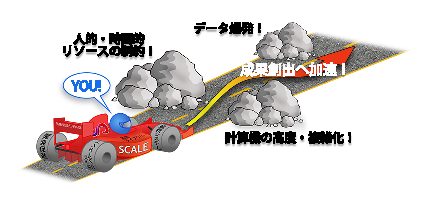
\includegraphics[width=0.9\hsize]{./figure/library.eps}\\
  \caption{\scalelib のねらい}
  \label{fig:scale}
\end{center}
\end{figure}

\scalelib は、理化学研究所 計算科学研究機構(RIKEN AICS)を中心に
開発が進められている気象・気候科学計算向けのライブラリである。
図 \ref{fig:scale}に\scalelib の思想の概念図を示す。
この図に示されるような諸問題に対応することを目指している。
\scalelib は次世代のスーパーコンピュータから小型PCクラスターに至るまで
広く用いられる事を念頭において開発されており、
気候・気象科学を専門とする科学者と計算機科学を専門とする科学者が
共同で開発を行っている。
そのため、スーパーコンピュータ「京」や富士通FX10等の
スーパーコンピュータに加え、インテル機のような汎用計算機でも
計算効率がでることを目指して設計されている。

\scalelib を利用した数値モデルとして、\scalerm が含まれている(図 \ref{fig:scale-rm})。
並列プロセスの管理、ファイル入出力、プロセス間通信や格子情報の設定は\scalelib が提供する。
大気流体の支配方程式を解く部分(流体力学コア、力学過程)と
雲微物理や大気放射のような諸物理過程を解く部分も\scalelib が提供する。
\scalerm は入力された大気状態のデータ(予報変数)を保持し、\scalelib が提供する機能を組み合わせ、
各コンポーネントを適切に呼び出すことで時間発展計算を行っている。
ユーザは必要に応じて利用するコンポーネントを選択し、組み合わせてシミュレーションを行うことが出来る。

\begin{figure}[hbt]
\begin{center}
  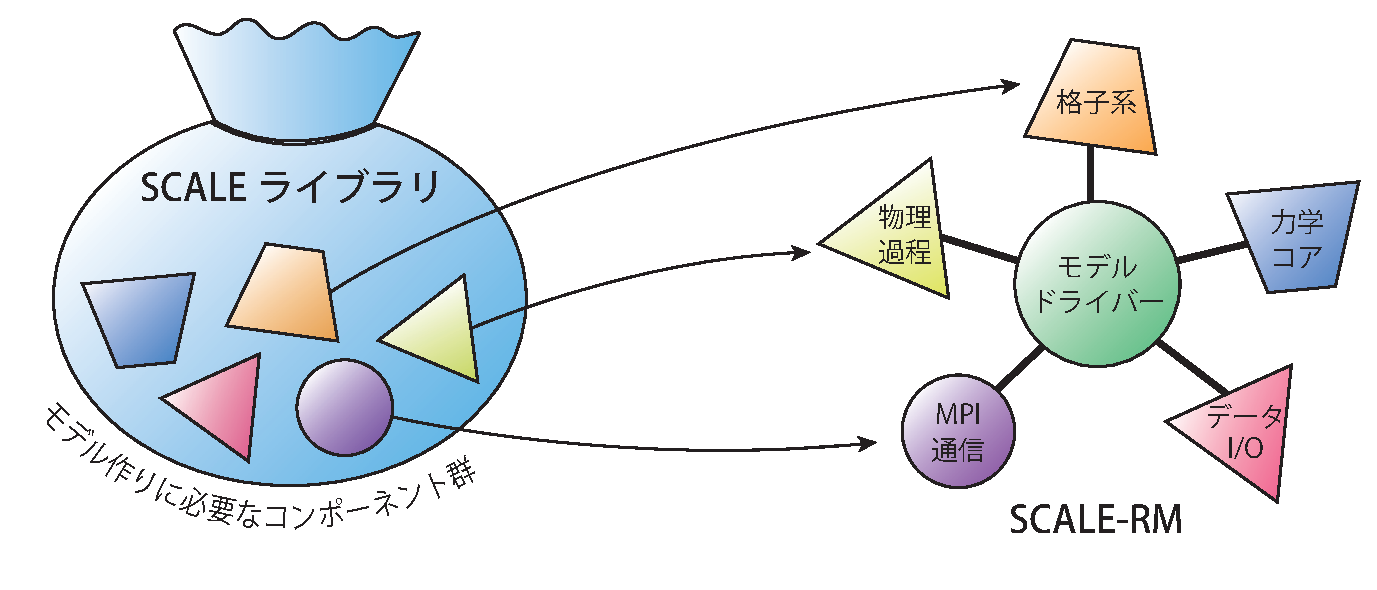
\includegraphics[width=0.9\hsize]{./figure/scale.eps}\\
  \caption{SCALEとSCALE-RMの関係}
  \label{fig:scale-rm}
\end{center}
\end{figure}



\subsection{\scalerm の構成}  \label{subsec:sturcture_scale_rm}
%--------------------------------------------------------------%
現在、\scalerm には下記のコンポーネントが実装されている。
\scalerm ではすべてのコンポーネントが利用可能である。
詳細なモデル構成や差分化手法については、
\citet{scale_2015}、\citet{satoy_2015b}、
および\citet{nishizawa_2015}を参照されたい。\\

{\bf フレームワーク}
\begin{itemize}
 \item 距離座標に基づいた三次元カーテシアン格子系
 \item MPI通信を用いた二次元領域分割
 \item 各種地図投影法
 \item ネスティングシステム(1 way:親領域$\to$子領域)
   \begin{itemize}
    \item オンライン実行(複数ドメインの計算を同時に実行)
    \item オフライン実行(外側ドメインの計算終了後に、その結果を用いて内側ドメインの計算を行う)
   \end{itemize}
 \item 複数事例一括実行 システム(バルクジョブシステム)
 \item CF 規約\footnote{\url{http://cfconventions.org/}}に基づく \netcdf ファイル I/O
   \begin{itemize}
   \item {\netcdf}3 または {\netcdf}4 形式
   \end{itemize}
 \item 理想実験のための初期値データ生成
 \item 外部データ読み込みによる標高・土地利用区分データの変換作成
 \item 外部データ読み込みによる初期値・境界値データ変換作成
   \begin{itemize}
    \item 
      WRF-ARW\footnote{\url{http://www.wrf-model.org/}}、
%      NICAM\footnote{\url{http://nicam.jp/}}、
      \grads \footnote{\url{http://cola.gmu.edu/grads/}}フォーマットでの入力に対応
   \end{itemize}
\end{itemize}

{\bf 力学コア関係}
\begin{itemize}
 \item 方程式系: 3次元完全圧縮非静力学方程式系
 \item 数値解法: 陽解法と陰解法の両方を実装
   \begin{itemize}
    \item 水平陽解法-鉛直陽解法
    \item 水平陽解法-鉛直陰解法
%    \item HI-VI(陰解法)
   \end{itemize}
 \item 空間差分: フラックス形式
    \begin{itemize}
      \item 2次中央差分
      \item 4次中央差分
      \item 6次中央差分
      \item 3次風上差分
      \item 5次風上差分
    \end{itemize}
 \item 時間差分:(詳細は、\citet{scale_2015}を参照のこと)
    \begin{itemize}
      \item Heun型3次ルンゲクッタスキーム
      \item \citet{Wicker_2002}の3段ルンゲクッタスキーム
      \item 4次ルンゲクッタスキーム
    \end{itemize}
 \item 非負保証:
    \begin{itemize}
      \item フラックス修正法 \citep[Flux Corrected Transport, FCT; ][]{zalesak_1979}
      \item \citet{Koren_1993}フィルター  (3次風上差分スキーム使用時のみ)
    \end{itemize}
 \item 数値フィルター: 4次超粘性・拡散
 \item 地形: 地形に沿った座標系
\end{itemize}

{\bf 物理過程}
\begin{itemize}
 \item 乱流過程: 複数から選択可能
   \begin{itemize}
    \item \citet{smagorinsky_1963} \& \citet{lilly_1962}型のサブグリッドモデル (\citet{Brown_etal_1994}と\citet{Scotti_1993}による補正)
    \item \citet{Deardorff_1980} サブグリッドモデル
    \item \citet{my_1982,nakanishi_2004}によるMYNN2.5境界層モデル
   \end{itemize}
 \item 雲微物理: 複数から選択可能
   \begin{itemize}
    \item \citet{kessler_1969}による3-class 1モーメントバルクモデル
    \item \citet{tomita_2008}による6-class 1モーメントバルクモデル
    \item \citet{sn_2014}による6-class 2モーメントバルクモデル
    \item \citet{suzuki_etal_2010}によるビン法モデル
   \end{itemize}
 \item 放射過程: \citet{sekiguchi_2008}による相関k分布法ブロードバンド大気放射伝達モデル
 \item 地表面モデル
  \begin{itemize}
   \item 陸面モデル: 熱拡散・バケツモデル
   \item 海洋モデル: 初期値固定・外部データ入力・スラブモデル
   \item 都市モデル: \citet{kusaka_2001}による単層キャノピーモデル
   \item バルク交換係数(陸面および海面): \citet{beljaars_1991,wilson_2001}による普遍関数によるバルク法
     もしくは \citet{uno_1995}によるLouis 型バルク法
  \end{itemize}
\end{itemize}



%==============================================================%
本書中では、Unix システム上のシェルである「 bash 」での実行を想定している。
異なる環境下では、適宜コマンドを読み替えて対応されたい。
また、本書内では特に断りがない限り、下記の表記法に従うものとする。

コマンドラインのシンボル(\verb|$, #|)は、コマンドの実行を示す。
以下のように、2つの表記の違いはプログラムの実行権限の違いを表す。

\begin{verbatim}
 #        <- root権限で実行するコマンド
 $        <- ユーザ権限で実行するコマンド
\end{verbatim}
%権限の一時的な切り替えにはsuコマンドを用いる。
%\verb|{User_Name}|は実際のユーザ名に読み替えること。
%\begin{verbatim}
% $ su {User_Name}   <- {User_Name}のユーザ名でログイン
% $ exit             <- {User_Name}のユーザ名でログインを終了
% $ su -             <- root権限に変更
% #
%\end{verbatim}

%コマンドオプションにハイフンを用いると、そのユーザでのログインを行う。
%用いない場合、権限のみの変更となる。またユーザ名を省略するとrootでのログインを試す。
%ユーザの一時切り替えを終わるには、exitコマンドを用いる。
%各プログラムをインストールするための圧縮ファイルは、/tmpにダウンロードされていると仮定する。
%他のディレクトリにダウンロードしてある場合は、mvコマンド等を用いて/tmpに移動しておくことを勧める。
%文章表記のうち、ダブルスラッシュ(//)で始まる行は解説のためのもので、実際に記述する必要はない。

下記に示すように、四角い囲みで区切られた記述は、コマンドラインのメッセージ部分を表す。\\
\msgbox{
 -- -- -- -- コマンドラインのメッセージ\\
 -- -- -- -- -- -- -- -- コマンドラインのメッセージ\\
 -- -- -- -- -- -- -- -- -- -- -- -- コマンドラインのメッセージ\\
}

一方、下記のように丸い囲みで区切られた記述は、エディタでファイルを編集する記述内容、
もしくはファイル内の記述の引用を表す。\\
\editbox{
 -- -- -- -- ファイル中の記述\\
 -- -- -- -- -- -- -- -- ファイル中の記述\\
 -- -- -- -- -- -- -- -- -- -- -- -- ファイル中の記述\\
}

本書では、FORTRAN のネームリストを\namelist{namelist}、
その項目を\nmitem{item_of_namelist}のように表記する。


\chapter{インストール} \label{chap:install}
%%%%%%%%%%%%%%%%%%%%%%%%%%%%%%%%%%%%%%%%%%%%%%%%%%%%%%%%%%%%%%%%%%%%%%%%%%%%%%%%%%%%%%
%  File 21_install.tex
%%%%%%%%%%%%%%%%%%%%%%%%%%%%%%%%%%%%%%%%%%%%%%%%%%%%%%%%%%%%%%%%%%%%%%%%%%%%%%%%%%%%%%

本章では、\scalelib と\scalerm のコンパイル及び、実行に必要な環境について説明する。

\section{必要なシステム環境} \label{sec:req_env}
%====================================================================================

\noindent {\bf 推奨のシステム環境}
\begin{itemize}
  \item {\bf システムハードウェア構成}\\
必要なハードウェアは実験設定に依存するが、
ここでは第\ref{chap:tutorial_ideal}章と第\ref{chap:tutorial_real}章の
チュートリアル実行に必要なスベックを示す。
  \begin{itemize}
    \item {\bf CPU} : 理想実験は物理コアが2コア以上、現実大気実験は4コア以上が望ましい。
    \item {\bf Memory} : 理想実験は512MB以上、現実大気実験は2GB以上のメモリ容量が必要 (倍精度浮動小数点使用時)。
    \item {\bf HDD} : 現実大気実験には約3GBのディスク空き容量が必要。
  \end{itemize}

  \item {\bf システムソフトウェア構成}
  \begin{itemize}
  \item {\bf OS} : Linux OS、Mac OS X\\
        対応確認済みOSについては、表\ref{tab:compatible_os}を参照のこと。
  \item {\bf コンパイラ} : Cコンパイラ、Fortran\\
        FortranコンパイラはFortran2003をサポートするコンパイラを必要とする。
        対応確認済みコンパイラについては、表\ref{tab:compatible_compiler}を参照のこと。
  \item {\bf MPIライブラリ} : MPI1.0/2.0 に対応するMPIライブラリを必要とする。
        対応確認済みMPIライブラリについては、表\ref{tab:compatible_mpi}を参照のこと。
  \item {\bf ファイルI/Oライブラリ} : gzip、HDF5、netCDF4を必要とする。\\
        HDF5/netCDF4の代わりに、netCDF3でも動作するが、出力ファイルサイズが大きくなる。
  \end{itemize}
\end{itemize}


\noindent {\bf あると便利なシステム環境}
\begin{itemize}
  \item {\bf データ変換ツール}:wgrib、wgrib2やNCLにより、\scalerm で読込可能な入力データの作成が可能である。チュートリアルの現実大気実験では、wgribを使用する。
  \item {\bf 描画環境}:\grads \footnote{\url{http://cola.gmu.edu/grads/}}、
GPhys/Ruby-DCL\footnote{\url{https://www.gfd-dennou.org/arch/ruby/products/gphys/}}、
ncview\footnote{\url{http://meteora.ucsd.edu/~piece/ncview\_home\_page.html}}など。
  \item {\bf 演算性能評価}:PAPIライブラリ\footnote{\url{http://icl.utk.edu/papi/}}が使用可能。
\end{itemize}


\begin{table}[htb]
\begin{center}
\caption{対応確認済みOS(全てx86-64の64bit版)}
\begin{tabularx}{150mm}{|l|l|X|} \hline
 \rowcolor[gray]{0.9} OS名 & 確認済みバージョン & 備考 \\ \hline
 CentOS                & 6.6、6.9、7.0、7.2、7.3 &  \\ \hline
 openSUSE              & 13.2、42.1、42.2        &  \\ \hline
 SUSE Enterprise Linux & 11.3、12.1         &  \\ \hline
 fedora                & 24、25、26         &  \\ \hline
 Mac OS X              & 10.11 (El Capitan) &  \\ \hline
\end{tabularx}
\label{tab:compatible_os}
\end{center}
\end{table}

\begin{table}[htb]
\begin{center}
\caption{対応確認済みコンパイラ}
\begin{tabularx}{150mm}{|l|X|X|} \hline
 \rowcolor[gray]{0.9} コンパイラ名 & 確認済みバージョン & 備考 \\ \hline
 GNU (gcc/gfortran)    & 4.4.7、4.7.4、4.8.5、4.9.4、6.1.1、6.3.1、7.1.1 & 4.3以前は非対応。4.4.xではコンパイル時にWarningが出ることがある。OpenMP対応。 \\ \hline
 Intel (icc/ifort)     & 13.0.1、14.0.2、16.0.1、17.0.1、17.0.2 & 2013年以降のバージョンを推奨。OpenMP対応。 \\ \hline
 PGI (gcc/pgfortran)   & 17.1                   & OpenACC対応 \\ \hline
\end{tabularx}
\label{tab:compatible_compiler}
\end{center}
\end{table}

\scalelib のソースコードはFortran2003規格に基づく機能を利用している。
そのため、Fortran2003の基本的な機能をサポートしたコンパイラが必要となる。
例えばGNU gfotranの場合、バージョン4.3以前ではFortran2003規格のサポートが不十分であるため、
\scalelib の利用環境として用いることは出来ない。

\begin{table}[htb]
\begin{center}
\caption{対応確認済みMPIライブラリ}
\begin{tabularx}{150mm}{|l|X|X|} \hline
 \rowcolor[gray]{0.9} MPIライブラリ名 & 確認済みバージョン & 備考 \\ \hline
 openMPI   & 1.7.2、1.8.1、1.10.2、1.10.3、1.10.5、1.10.7、2.0.2、2.1.0、2.1.1 & \\ \hline
 Intel MPI & 4.1.0、5.1.2、2017.2 & 2013年以降のバージョンを推奨 \\ \hline
 SGI MPT   & 2.09、2.14               & Intel Compilerとの組み合わせで確認済み \\ \hline
\end{tabularx}
\label{tab:compatible_mpi}
\end{center}
\end{table}

以上で説明したもの以外に、\scalelib は、
理化学研究所 計算科学研究機構のスーパーコンピュータ「京」
の環境でも動作確認されている。


\section{ライブラリ環境のインストール} \label{sec:inst_env}
%====================================================================================
\scalelib ライブラリに必要な各種ライブラリ(FortranおよびCコンパイラ、MPI、NetCDF、HDF5 等)
のインストールを行う。
詳細は、付録 \ref{achap:env_setting}章を参照のこと。
第\ref{chap:tutorial_ideal}章、第\ref{chap:tutorial_real}章のチュートリアルは、
それらのライブラリ環境がインストールされていることを前提として進める。

描画ツールとして、
第\ref{chap:tutorial_ideal}章、第\ref{chap:tutorial_real}章のチュートリアルでは
クイックビューのためGPhysを使用する。
また、\grads を使った結果の描画方法についても紹介する。
これらの描画ツールの詳細とインストール方法については
付録 \ref{sec:env_vis_tools}を参照のこと。



\section{\scalelib のコンパイル} \label{sec:scale_compile}
%====================================================================================

以下の説明で使用した環境は次のとおりである。
\begin{itemize}
\item CPU: Intel Core i5 2410M 2コア/4スレッド
\item Memory: DDR3-1333 4GB
\item OS: CentOS 6.6 x86-64、CentOS 7.1 x86-64、openSUSE 13.2 x86-64
\item GNU C/C++、Fortran compiler (付録\ref{achap:env_setting}章参照)
\end{itemize}

\subsection{ソースコードの入手} \label{subsec:get_source_code}
%-----------------------------------------------------------------------------------
最新のリリース版ソースコードは、\\
\url{http://scale.aics.riken.jp/ja/download/index.html}\\
よりダウンロードできる。
ソースコードのtarballファイルを展開すると\texttt{scale-{\version}/} というディレクトリができる。
\begin{alltt}
 $ tar -zxvf scale-{\version}.tar.gz
 $ ls ./
    scale-{\version}/
\end{alltt}

\subsection{Makedefファイルと環境変数の設定} \label{subsec:evniromnet}
%-----------------------------------------------------------------------------------

\scalelib はコンパイルするとき、環境変数``\verb|SCALE_SYS|''に設定した
Makedefファイルを使用してコンパイルが行われる。
Makedefファイルは、\texttt{scale-{\version}/sysdep/}内にいくつかの計算機環境に
対応するファイル(\texttt{Makedef.***})が準備されており、
これらの中から自分の環境にあったものを設定する。
動作確認済みの環境と対応するMakedefファイルを表\ref{tab:makedef}に示す。
自分の環境に合致するものがなければ、既存ファイルをベースに各自作成する。

\begin{table}[htb]
\begin{center}
\caption{環境例と対応するMakedefファイル}
\begin{tabularx}{150mm}{|l|l|X|l|} \hline
 \rowcolor[gray]{0.9} OS/計算機 & コンパイラ & MPI & Makedefファイル \\ \hline
                 & gcc/gfortran & openMPI & Makedef.Linux64-gnu-ompi \\ \cline{2-4}
 Linux OS x86-64 & icc/ifort & intelMPI & Makedef.Linux64-intel-impi \\ \cline{2-4}
                 & icc/ifort    & SGI-MPT & Makedef.Linux64-intel-mpt \\ \hline
 Mac OS X        & gcc/gfortran & openMPI & Makedef.MacOSX-gnu-ompi \\ \hline
 スーパーコンピュータ「京」 & fccpx/frtpx & mpiccpx/mpifrtpx & Makedef.K \\ \hline
 Fujitsu PRIME-HPC FX10 & fccpx/frtpx & mpiccpx/mpifrtpx & Makedef.FX10 \\ \hline
\end{tabularx}
\label{tab:makedef}
\end{center}
\end{table}


Linux OS、GNUコンパイラ、openMPIを使用する場合には、
\verb|"Makedef.Linux64-gnu-ompi"|が対応するファイルとなる。
別の環境でインストールを行っている場合には、適宜、表\ref{tab:makedef}に従って読み替えること。
下記の通り、環境変数を設定する。
\begin{alltt}
 $ export SCALE_SYS="Linux64-gnu-ompi"
\end{alltt}
実行環境が常に同じであるならば、
環境変数の設定を\verb|.bashrc|などの環境設定ファイルに
記述しておくと便利である。\\


各種ライブラリのインストールを
付録\ref{achap:env_setting}章に従って行った場合を除き、
下記のPATHの設定が必要となる。
HDF5とNetCDF4については、下記のように環境変数を設定する。
例えば、Intel コンパイラを利用して、
HDF5を\verb"/opt/hdf5"、NetCDF4を\verb|/opt/netcdf|に
それぞれインストールした場合の例を示す。
適宜、各自の環境に応じて読み替えて設定すること。
\begin{verbatim}
 $ export SCALE_NETCDF_INCLUDE="-I/opt/netcdf/include"
 $ export SCALE_NETCDF_LIBS="-L/opt/hdf5/lib64 -L/opt/netcdf/lib64 -lnetcdff -lnetcdf -hdf5_hl -lhdf5 -lm -lz"
\end{verbatim}


\subsection{コンパイル} \label{subsec:compile}
%-----------------------------------------------------------------------------------

\scalerm ソースディレクトリに移動して、makeコマンドによってコンパイルを行う。
\begin{alltt}
 $ cd scale-{\version}/scale-rm/src
 $ make -j 4
\end{alltt}
\verb|make|のあとの \verb|"-j 4"| は、
コンパイル時の並列数(例では4並列)を示しており、
実行環境によって並列数を指定すれば良い。
コンパイルが成功すると下記3つの実行ファイルがscale-{\version}/bin 以下に生成される。
\begin{alltt}
 scale-rm  scale-rm_init  scale-rm_pp
\end{alltt}


また、コンパイルをやり直したい場合など、下記のコマンドで作成された実行バイナリを消去できる。
\begin{alltt}
 $ make clean
\end{alltt}
ただし、この場合、コンパイルされたライブラリは消去されないため、
全てのコンパイル済みファイルを消去したい場合は、
\begin{alltt}
 $ make allclean
\end{alltt}
とする。
コンパイル環境、コンパイルオプションを変更して再コンパイルする場合は、
``allclean''を実行すること。\\



{\bf 注意点}
\begin{itemize}
\item \scalelib は、scaleのTOPディレクトリ直下の
 scale-{\version}/scalelib/ というディレクトリ内でコンパイルとアーカイブが行われる。
 \scalerm は、コンパイルを実行したディレクトリの下の
 \verb|".lib"|という名前の隠しディレクトリの中にコンパイルされたオブジェクトファイルが置かれる。
% 実行バイナリファイルはカレントディレクトリにコピーされる。
\item Debugモードでコンパイルしたい場合は、\verb|"make -j 4 SCALE_DEBUG=T"|としてコンパイルする。
 (コンパイル時に適用される全ての環境変数リストは表\ref{tab:env_var_list}を参照)
\item 細かくコンパイルオプションを変更したい場合は、\verb|Makedef.***|のファイルを編集する。
\end{itemize}

\begin{table}[htb]
\begin{center}
\caption{コンパイル時の環境変数のリスト}
\begin{tabularx}{150mm}{|l|X|} \hline
 \rowcolor[gray]{0.9} 環境変数 & 説明  \\ \hline
 SCALE\_SYS               & システム選択(必須)  \\ \hline
 SCALE\_DISABLE\_MPI      & MPIを使わない(utilsのみ)  \\ \hline
 SCALE\_DEBUG             & デバッグ用コンパイルオプションでコンパイル  \\ \hline
 SCALE\_QUICKDEBUG        & クイックデバッグ用コンパイルオプション利用(高速化そのまま+浮動小数点エラー検出)  \\ \hline
 SCALE\_USE\_MASSCHECK    & 質量保存チェック用の計算を追加(RM力学過程のみ)  \\ \hline
 SCALE\_USE\_SINGLEFP     & 単精度浮動小数点を使用(原則として全ソース)  \\ \hline
 SCALE\_USE\_FIXEDINDEX   & 格子サイズをコンパイル時に固定して最適化促進  \\ \hline
 SCALE\_ENABLE\_OPENMP    & OpenMP機能を有効にする  \\ \hline
 SCALE\_ENABLE\_OPENACC   & OpenACC機能を有効にする  \\ \hline
 SCALE\_USE\_AGRESSIVEOPT & 副作用が出る可能のある強い最適化まで行う(京・FXのみ)  \\ \hline
 SCALE\_DISABLE\_INTELVEC & ベクトル化オプションの抑制(インテルコンパイラのみ)  \\ \hline
 SCALE\_NETCDF\_INCLUDE   & NetCDFライブラリのincludeディレクトリパス  \\ \hline
 SCALE\_NETCDF\_LIBS      & NetCDFライブラリのディレクトリパスとライブラリ指定  \\ \hline
 SCALE\_ENABLE\_PNETCDF   & parallel NetCDFを利用する  \\ \hline
 SCALE\_COMPAT\_NETCDF3   & NetCDF3互換の機能に限定する  \\ \hline
 SCALE\_ENABLE\_MATHLIB   & 数値計算ライブラリを利用する  \\ \hline
 SCALE\_MATHLIB\_LIBS     & 数値計算ライブラリのディレクトリパスとライブラリ指定  \\ \hline
 SCALE\_ENABLE\_PAPI      & PAPIを利用する  \\ \hline
 SCALE\_PAPI\_INCLUDE     & PAPIライブラリのincludeディレクトリパス  \\ \hline
 SCALE\_PAPI\_LIBS        & PAPIライブラリのディレクトリパスとライブラリ指定  \\ \hline
 SCALE\_DISABLE\_LOCALBIN & テストケースディレクトリに特別版のバイナリが作られないようにする  \\ \hline
 SCALE\_IGNORE\_SRCDEP    & コンパイル時にソースコードの依存関係確認を行わない  \\ \hline
 SCALE\_ENABLE\_SDM       & 超水滴モデルを利用する   \\ \hline
\end{tabularx}
\label{tab:env_var_list}
\end{center}
\end{table}

\section{後処理ツール(net2g)のコンパイル} \label{sec:source_net2g}
%====================================================================================

\scalerm の出力ファイルは、ノードごとに分割されて出力される。
\scalelib では、これら出力ファイル(\verb|history.******.nc|)を結合し、
\grads で直接読み込めるデータ形式へ
変換する後処理ツール「net2g」を提供している。
第\ref{chap:tutorial_ideal}章、第\ref{chap:tutorial_real}章のチュートリアルでも使用する。
ここでは、net2gのコンパイル方法について説明する。

%net2gはSCALE本体から独立したツールになっている
%(ただしMakedefファイルを除く)ため、
%任意の場所へコピーしてコンパイルすることができるが、
%コンパイルにはnetCDFライブラリが必要であり、
%また並列実行するためにはMPIライブラリが必要である。
%従って、以降はこれらのライブラリがインストールされている環境であることを想定して進める。\\


まず、SCALE本体のコンパイル時と同様に、
使用する環境にあったMakedefファイル設定のための環境変数を設定する
(\ref{subsec:compile}節コンパイル参照)。
次に、net2gのディレクトリに移動し、makeする。
MPIライブラリを用いた並列実行を行うためのバイナリは、
下記のコマンドによって生成される。
\begin{alltt}
 $ cd scale-{\version}/scale-rm/util/netcdf2grads_h
 $ make -j 2
\end{alltt}
MPIライブラリが無い場合など、逐次実行バイナリを生成するためには、
\begin{alltt}
 $ make -j 2 SCALE_DISABLE_MPI=T
\end{alltt}
としてコンパイルを行う。
\verb|net2g|という名前の実行ファイルが生成されていればコンパイルは成功である。\\


下記のコマンドで作成された実行バイナリを消去できる。
\begin{alltt}
 $ make clean
\end{alltt}

%%%%%%%%%%%%%%%%%%%%%%%%%%%%%%%%%%%%%%%%%%%%%%%%%%%%%%%%%%%%%%%%%%%%%%%%%%%%%%%%%%%%%%



\chapter{動作確認と基本的な操作について} \label{chap:tutorial_ideal}
%%%%%%%%%%%%%%%%%%%%%%%%%%%%%%%%%%%%%%%%%%%%%%%%%%%%%%%%%%%%%%%%%%%%%
%  File 31_ideal_exp.tex
%%%%%%%%%%%%%%%%%%%%%%%%%%%%%%%%%%%%%%%%%%%%%%%%%%%%%%%%%%%%%%%%%%%%%
\section{Introduction} \label{sec:ideal_exp_intro}

In this chapter, the basic operations of SCALE-RM for numerical experiments are explained. For this purpose, an ideal experiment case is prepared. It is strongly recommend that the user perform this tutorial because it includes a check for whether the compilation of SCALE  in Part \ref{part:install} has been completed. This chapter assumes that the following file has been already generated:
\begin{alltt}
  scale-{\version}/bin/scale-rm
  scale-{\version}/bin/scale-rm_init
  scale-{\version}/bin/sno
\end{alltt}
Furthermore, \grads is used as a drawing tool. ``gpview'' can also be used for the confirmation of the result. Refer to Section \ref{sec:inst_env} for their installation procedures.

The tutorial is described in order of preparation: creating the initial data, conducting the simulation, post-processing the output, and drawing the results.



\section{モデルの実行方法} \label{sec:ideal_exp_run}
%====================================================================================

\subsubsection{実験設定}
%====================================================================================

理想実験のチュートリアルとして、ここでは、2次元モデルにおける積雲対流の理想実験を実施する。
この実験では、典型的な大気の鉛直分布と対流圏下層に初期擾乱を与えて、
積乱雲が発生し発達する過程を計算する。
表\ref{tab:setting_ideal}に、実験設定を示す。

\begin{table}[htb]
\begin{minipage}{150mm}
\begin{center}
\caption{理想実験の実験設定}
\begin{tabularx}{150mm}{|l|X|X|} \hline
 \rowcolor[gray]{0.9} 項目 & 設定内容 & 備考 \\ \hline
 MPIプロセス数 & 東西:1、南北:2 & 計2プロセスによる並列計算 \\ \hline
 水平格子間隔 & 東西:500 m、南北:500 m & 南北-鉛直面を切り取った2次元実験 \\ \hline
 水平格子点数 & 東西:1、南北:40 &  \\ \hline
 鉛直層数     & 97層(モデル上端: 20 km)& 下層ほど層厚を細かく切ったストレッチ格子を使用 \\ \hline
 側面境界条件 & 周期境界 & 東西、南北方向の両方に適用 \\ \hline
 時間刻み幅   & 5 sec      & 雲微物理スキームに対しては 10 sec \\ \hline
 積分期間     & 3,600 sec  & 合計で 720 ステップ  \\ \hline
 データ出力間隔 & 300 sec  &  \\ \hline
 物理スキーム & 雲微物理スキームのみ使用 &
 6-class single moment bulk model \citep{tomita_2008} \\ \hline
 初期の鉛直分布 & GCSS Case1 squall-line \citep{Redelsperger2000}&
 風の分布は、\citet{Ooyama_2001}に基づいた鉛直シアを設定 \\ \hline
 初期擾乱 & 暖気塊(warm bubble) & 半径: 水平 4 km、
 鉛直 3 km. 極大値: 3 K. \\ \hline
\end{tabularx}
\label{tab:setting_ideal}
\end{center}
\end{minipage}
\end{table}


\subsubsection{準備} %\label{subsec:ideal_exp_prepare}
%------------------------------------------------------
理想実験は、ディレクトリ\verb|scale-rm/test/tutorial/ideal|の中で実行する。
このディレクトリに移動し、scale-{\version}/bin にある実行バイナリへのシンボリックリンクを張る。
\begin{alltt}
  $ cd scale-rm/test/tutorial/ideal
  $ ln -s ../../../../bin/scale-rm      ./
  $ ln -s ../../../../bin/scale-rm_init ./
\end{alltt}
ここで、「\verb|scale-rm|」はモデル本体、
「\verb|scale-rm_init|」は初期値/境界値作成ツールである。

\subsubsection{初期値の作成} \label{subsec:ideal_exp_init}
%------------------------------------------------------
初期値の作成には、\verb|scale-rm_init|に与える設定ファイルが必要である。
設定ファイル\\ \verb|sample/init_R20kmDX500m.conf| には、表\ref{tab:setting_ideal} に対応する実験設定が書かれている。
この設定ファイルを読み込ませると、\verb|scale-rm_init|は大気の成層構造と初期擾乱を計算する。

\scalerm の実行コマンドの一般的な形式は、
\begin{alltt}
  $ mpirun  -n  [プロセス数]  [実行バイナリ名]  [設定ファイル]
\end{alltt}
である。
[プロセス数]にはMPI並列で使用したいプロセス数、
[実行バイナリ]には\verb|scale-rm|や\verb|scale-rm_init|といった実行バイナリ名を指定する。
[設定ファイル]には実験設定を記述した設定ファイルを指定する。
設定ファイルとして\verb|sample/init_R20kmDX500m.conf|を使用し、
2 プロセスによるMPI並列で\verb|scale-rm_init|を実行する場合には、
コマンドは
\begin{alltt}
  $ cp  sample/init_R20kmDX500m.conf ./init_R20kmDX500m.conf
  $ mpirun  -n  2  ./scale-rm_init  init_R20kmDX500m.conf
\end{alltt}
%
と記述する。
\noindent 実行が成功すれば、コマンドラインに以下のメッセージが表示される。\\

\noindent {\small {\gt
\fbox{
\begin{tabularx}{150mm}{l}
 *** Start Launch System for SCALE-RM\\
 *** Execute preprocess? :  T\\
 *** Execute model?      :  F\\
 *** End   Launch System for SCALE-RM\\
\end{tabularx}
}}}\\


\noindent この実行によって、下記の3つのファイルが、現在のディレクトリ下に作成される。
\begin{alltt}
  init_LOG.pe000000
  init_00000101-000000.000.pe000000.nc
  init_00000101-000000.000.pe000001.nc
\end{alltt}
計算領域の全体は、MPIプロセス数だけ水平方向に分割される。
ファイル名において\verb|pe|に続く番号は、MPIのプロセス番号を示している。
ログファイル(\verb|init_LOG.pe000000|)には、
コマンドラインには表示されない詳細な情報が記録されている。
この例では 2 つのMPIプロセスを使用しているが、
デフォルト設定では 0 番目のプロセス(マスターランク)に対するログファイルだけが出力される。
実行が正常に終了すれば、LOGファイルの最後に\\
\msgbox{
 +++++ Closing LOG file\\
}
が出力される。

\verb|init_00000101-000000.000.pe000000.nc|と\verb|init_00000101-000000.000.pe000001.nc|の2つのファイルは初期値ファイルであり、
それぞれ約 600 KBのファイルサイズになる。
ファイル名の末尾が「.nc」で終わるファイルは {\netcdf}形式のファイルであり、
GPhys/Ruby-DCL や ncview によって直接読み込める。


\subsubsection{シミュレーションの実行} \label{subsec:ideal_exp_run}
%------------------------------------------------------
プロセス並列数は、初期値の作成時と同じにする必要がある。
シミュレーションの実行用の設定ファイルは、\verb|sample/run_R20kmDX500m.conf| である。
\begin{alltt}
  $ cp  sample/run_R20kmDX500m.conf  ./run_R20kmDX500m.conf
  $ mpirun  -n  2  ./scale-rm  run_R20kmDX500m.conf
\end{alltt}

本書の必要要件にあった計算機であれば、2 分程度で計算が終わる。
この実行によって、3つのファイル
\begin{alltt}
  LOG.pe000000
  history.pe000000.nc
  history.pe000001.nc
\end{alltt}
が、現在のディレクトリ下に作成される。
実行が正常に終了すれば、LOGファイルの最後に
\msgbox{
 +++++ Closing LOG file\\
}
と出力される。
\verb|history.pe000000.nc| と \verb|history.pe000001.nc|
の2つのファイルは、計算結果を含むヒストリファイルである。
これらのファイル形式は{\netcdf}であり、各ファイルのサイズは約1.5 MBである。

\section{Post-processing and drawing} \label{sec:ideal_exp_net2g}
%------------------------------------------------------
In this section, we explain post-processing and the method of drawing the calculation result.  In the tutorial, the distributed files in \netcdf format are merged into one file and converted into simple binary form ({\grads} form) that can be directly accessed. The binary form makes it easy for users to analyze the result. Link to the post-processing tool \verb|net2g| compiled  in Section \ref{sec:source_net2g}:
\begin{verbatim}
  $ ln -s ../../../util/netcdf2grads_h/net2g  ./
\end{verbatim}

The method of execution of \verb|net2g| is the same as that of \scalerm, i.e.,
\begin{verbatim}
 $ mpirun -n [the number of the processes] ./net2g [the configuration file] 
\end{verbatim}
The configuration file \verb|net2g.conf| is intended for special uses of \verb|net2g|.
Give this configuration file to \verb|net2g| and execute it as follows:
\begin{verbatim}
  $ mpirun  -n  2  ./net2g  net2g.conf
\end{verbatim}
If there is no error message and the following message is displayed to the standard output,
the conversion is completed without problem:
\msgbox{
\verb|+++ MPI COMM: Corrective Finalize| \\
}

The execution of net2g should be handled,
so that the number of MPI processes is identical to, or a divisor of, that used for the run of \scalerm. The following six files are generated under the same directory by this execution:
\begin{alltt}
  QHYD_d01z-3d.ctl
  QHYD_d01z-3d.grd
  U_d01z-3d.ctl
  U_d01z-3d.grd
  W_d01z-3d.ctl
  W_d01z-3d.grd
\end{alltt}
The ``grd'' files are the converted files in the simple binary form of direct access
({\grads} form) obtained by merging the divided files,
whereas the ``ctl'' files are used to render them readable by \grads.
%In this case, these files contain U (horizontally eastern wind), W (vertical wind), and QHYD (mass concentration of total hydrometeors).

To confirm whether the calculation is satisfactory,
draw a figure using \grads script \verb|checkfig_ideal.gs|.
Note that the grammar depends on the version of \grads.
If a warning appears, the \grads script should be rewritten appropriately:
\begin{verbatim}
  $ grads -blc checkfig_ideal.gs
\end{verbatim}
If it is successfully completed, the following files are generated:

\begin{verbatim}
   ideal_QHYD.png
   ideal_W.png
\end{verbatim}
The same figures as Fig. \ref{fig_ideal} can be found in the simulation,
and post-processing is successfully concluded.

\begin{figure}[htb]
\begin{center}
  \includegraphics[width=0.65\hsize]{./figure/ideal_qhyd.eps}\\
  \includegraphics[width=0.65\hsize]{./figure/ideal_W.eps}\\
  \caption{The horizontal-vertical cross-section at Y=750m after t=1200 s (20 minutes later);
            The color indicates (a) the mass concentration of the hydrometeor and (b) vertical velocity. The vector indicates flow in both of figures.}
  \label{fig_ideal}
\end{center}
\end{figure}

To convert the result of the output into binary data for other variables,
add them to \nmitem{VNAME} in \namelist{VARI} in the configuration file \verb|net2g.conf|:
\editbox{
\verb|&VARI|\\
\verb| VNAME       = "U","W","QHYD"|\\
\verb|/|\\
}
To check the output variable in the history file, use \verb|ncdump| of {\netcdf}.
Refer to Section \ref{sec:net2g} for the detailed use of net2g. 


\section{応用に向けたガイドライン} \label{sec:ideal_exp_last}

本章では簡単な理想実験を例にして{\scalerm}の実行方法を説明した。
次の段階として、モデルの解像度、計算領域、MPIプロセス数を変更する方法を把握することを勧める。
本章の理想実験に関しては、この実験で使用したディレクトリ下にある「sample」ディレクトリの中に、
解像度設定、領域設定、物理スキーム等を変更した設定ファイルを数種類用意してある。
これらは、設定を変更する際に参考となるだろう。
また、ディレクトリ「\verb|scale-rm/test/case|」の下には、様々な理想実験に対する設定を用意している。
幾つかの理想実験については、それらの実験設定に特化したソースコードを必要とするため、
設定ファイルの存在するディレクトリで make コマンドを再度実行する必要がある。
初期値作成と実行の手順は、基本的に本章のチュートリアルと同じである。

雲微物理スキーム、放射スキーム、乱流スキーム等の物理過程の設定方法を確認することも重要である。
これらの変更方法は第\ref{part:basic_usel}章に記載されている。


\chapter{簡単な現実実験の方法} \label{chap:tutorial_real}
%-------------------------------------------------------%
\section{Overview} \label{sec:tutorial_real_intro}
%-------------------------------------------------------%
In this chapter, the basic execution procedure of the real atmospheric experiment is described using a simple case according to the workflow in Fig. \ref{fig:howto}.
\begin{enumerate}
\item Preparations for input data. The input data must be prepared by users themselves.
\item \texttt{pp}:   Making topographical data
\item \texttt{init}: Making initial and boundary data
\item \texttt{run}:  Executing the simulation
\item \texttt{sno}:  Converting {\netcdf} output data ( optional )
\end{enumerate}
Hereinafter, the absolute path \texttt{scale-{\version}/scale-rm/test/tutorial/} is denoted by\\
\verb|${Tutorial_DIR}|.

\begin{figure}[tb]
\begin{center}
  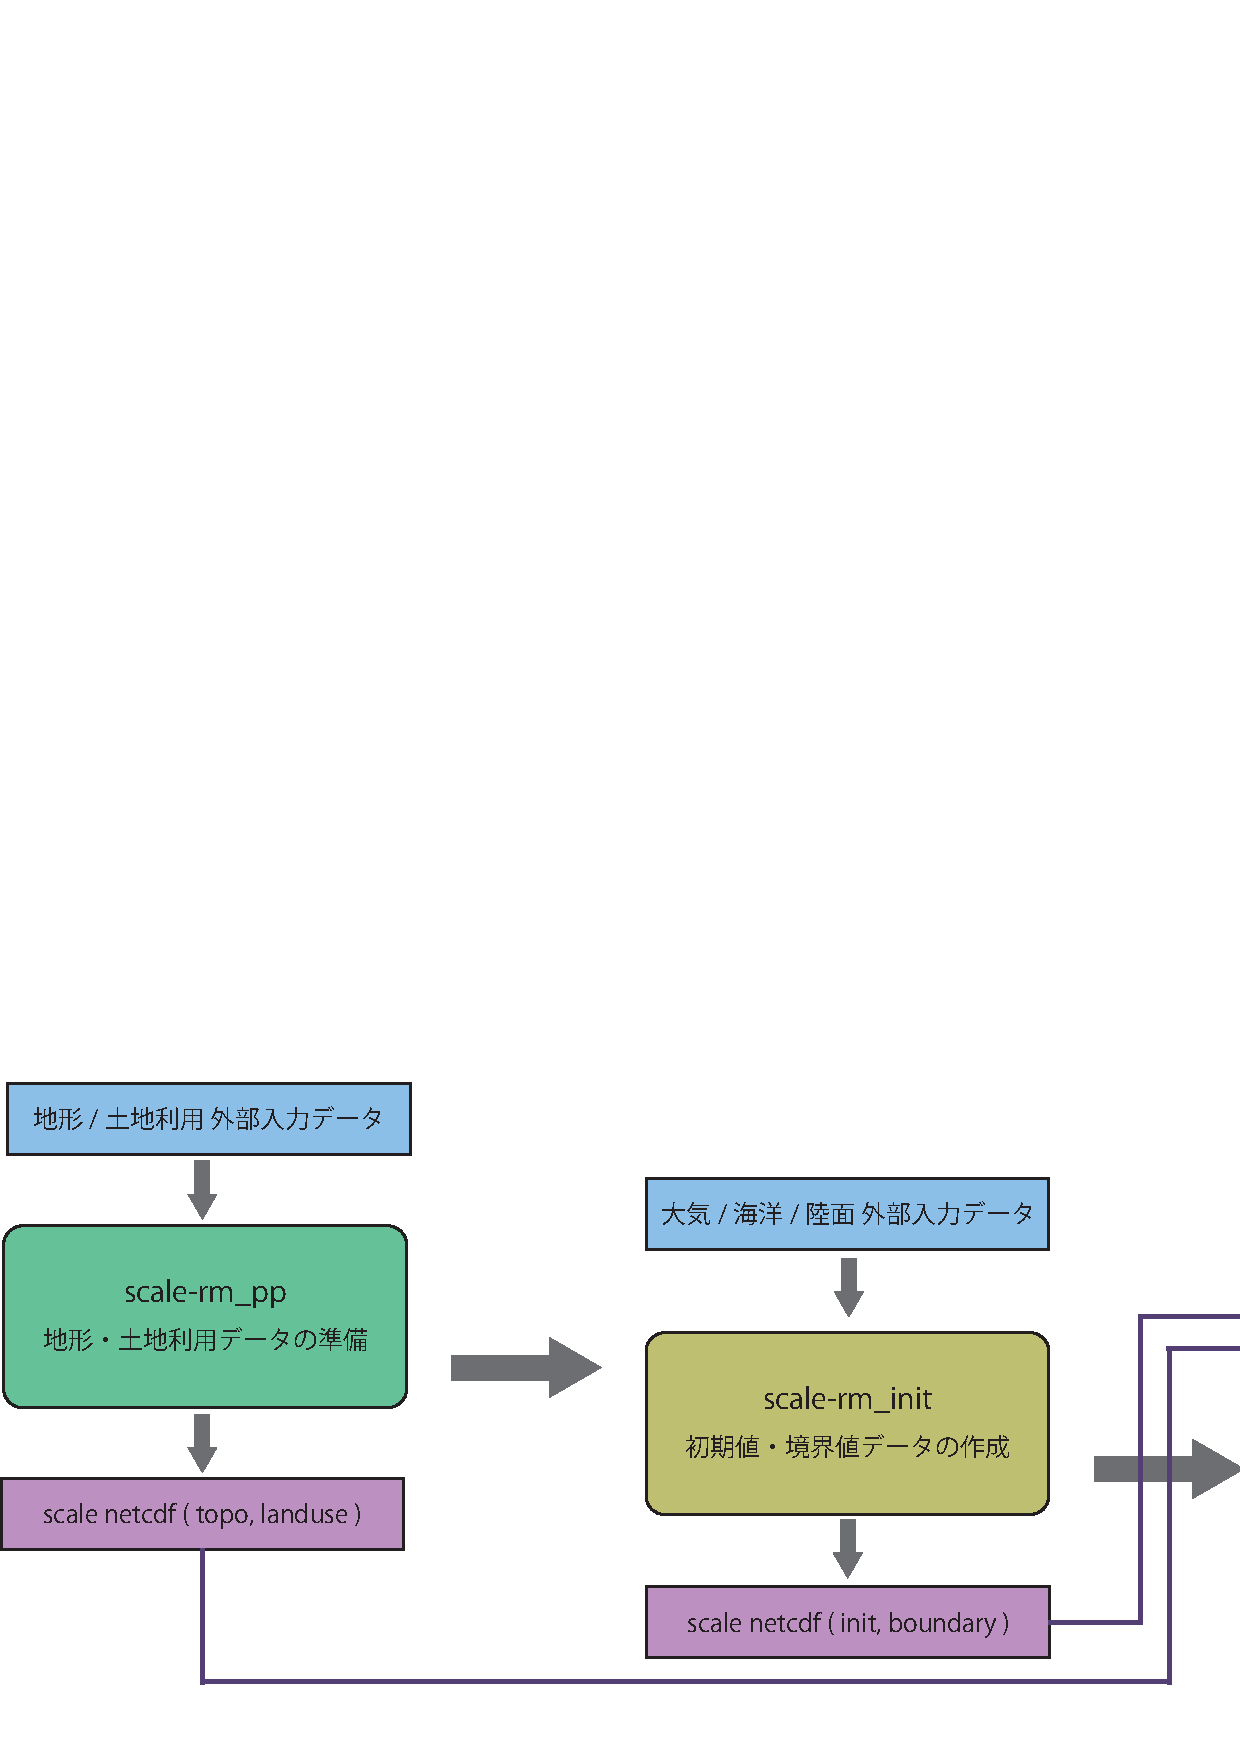
\includegraphics[width=0.9\hsize]{./../../figure/real_procedure.pdf}\\
  \caption{\scalerm procedure of model execution}
  \label{fig:howto}
\end{center}
\end{figure}

The settings for the calculation domain used in this tutorial are given in Table \ref{tab:grids}.
Figure \ref{fig:tutorial_real_domain} shows the target domain.
Since this tutorial focuses on learning how to conduct 
real atmospheric experiments using \scalerm quickly,
the experiment is designed to be completed in a short time.
Note that this setting may not be appropriate as a physically valid experiment, 
and in practical application one should examine the experimental setup as needed.

\begin{table}[tb]
\begin{center}
  \caption{Overview of experimental settings}
  \label{tab:grids}
  \begin{tabularx}{150mm}{|l|X|} \hline
    \rowcolor[gray]{0.9} Item & Configuration \\ \hline
    MPI process decomposition (east-west $\times$ north-south) & 2 $\times$ 2 (total: 4 processes) \\ \hline
    Number of horizontal grids (east-west $\times$ north-south) & 90 $\times$ 90  \\ \hline
    Number of vertical layers   & 36                   \\ \hline
    Horizontal grid intervals   & $\Delta x  = \Delta y = $ 20km       \\ \hline
    Integration period & July 14, 2007, 18UTC - July 15 00UTC (6 hour integration) \\ \hline
    Time step & 90 s/step (total:240 steps) \\ \hline
  \end{tabularx}
\end{center}
\end{table}

\begin{figure}[tb]
\begin{center}
  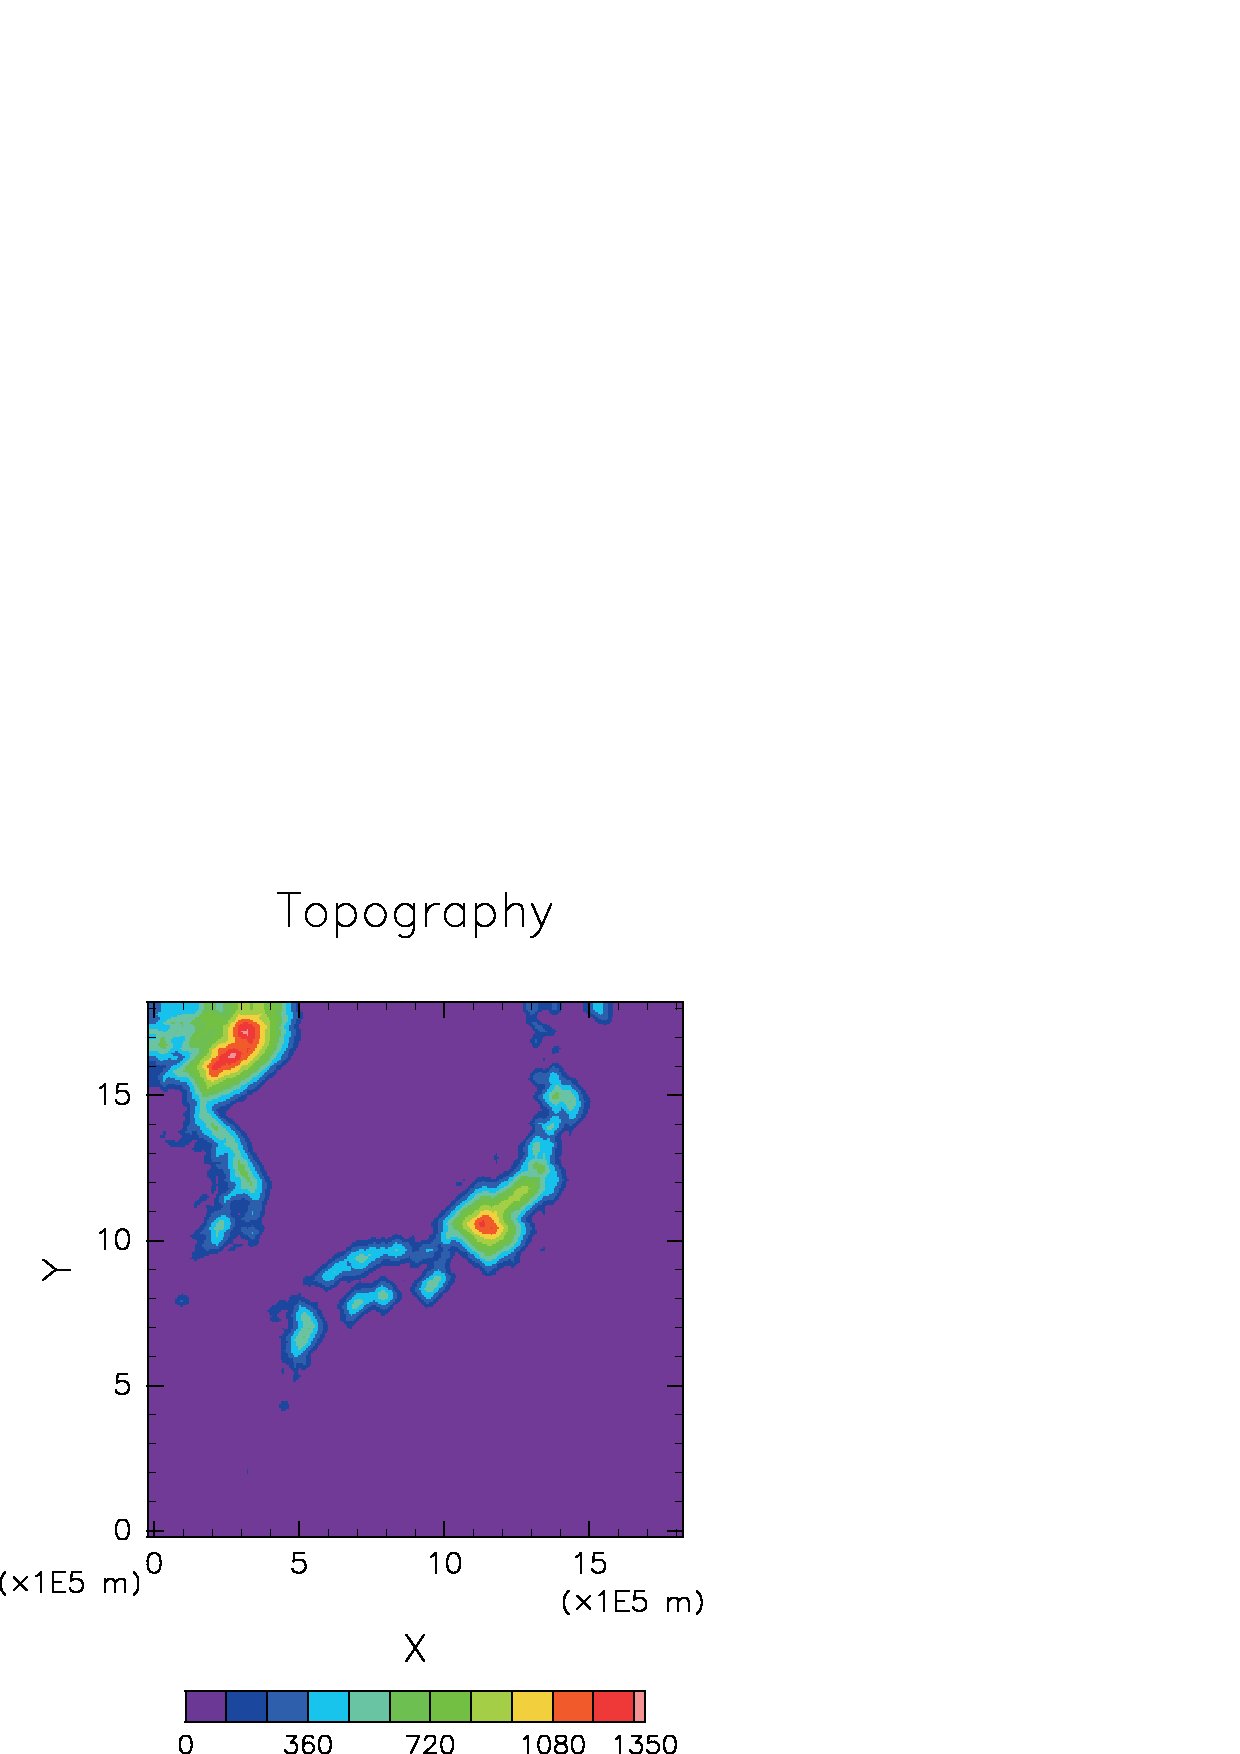
\includegraphics[width=0.95\hsize]{./../../figure/real_domain.pdf}\\
  \caption{Topographical and land-ocean distribution in the domain}
  \label{fig:tutorial_real_domain}
\end{center}
\end{figure}



%-------------------------------------------------------%
\section{Preparations for input data (boundary data)} \label{sec:tutrial_real_data}
%-------------------------------------------------------%

When a realistic atmospheric experiment is conducted, boundary data need to be provided to \scalerm. Table \ref{tab:real_bnd} shows the items for external input data to create boundary data. The variables denoted by {\color{blue}blue character} in this table  are always needed, whereas the others (black character) are optional.
\begin{table}[tb]
\begin{center}
  \caption{Items of external input data for real atmospheric experiments}
  \label{tab:real_bnd}
  \begin{tabularx}{150mm}{llX} \hline
    \rowcolor[gray]{0.9}
    \multicolumn{3}{l}{Data to create the topography and land-use data (in general, in-situ data)}\\ \hline
    & \multicolumn{2}{l}{\color{blue}{Altitude data}}\\
    & \multicolumn{2}{l}{\color{blue}{Land-use classification data}}\\ \hline
    \rowcolor[gray]{0.9}
    \multicolumn{3}{l}{data to craete the initial and boundary data for \scalerm (in general, GCM data)}\\ \hline
    &  \multicolumn{2}{l}{\color{blue}{Information for latitude and longitude of the parent model}}\\
    &  \multicolumn{2}{l}{--- 3D atmospheric data ---}\\
    &  & \multicolumn{1}{l}{\color{blue}{zonal and meridional winds, temperature, specific humidity (relative humidity),}} \\
    &  & \multicolumn{1}{l}{\color{blue}{pressure, geopotential height}} \\
    &  \multicolumn{2}{l}{--- 2D atmospheric data---}\\
    &  & \multicolumn{1}{l}{sea-level pressure, surface pressure, zonal and meridional wind at 10m,} \\
    &  &\multicolumn{1}{l}{temperature and specific humidity (relative humidity) at 2m} \\
    &  \multicolumn{2}{l}{--- 2D land data ---}\\
    & &  \multicolumn{1}{l}{land and sea map in the parent model}\\
    & &  \multicolumn{1}{l}{\color{blue}{surface skin temperature}}\\
    & &  \multicolumn{1}{l}{{\color{blue}{information of depth of soil data in the parent model, soil temperature,}}}\\
    & &  \multicolumn{1}{l}{{{soil moisture(volume content or degree of saturation)}}}\\
    &  \multicolumn{2}{l}{--- 2D ocean data at the surface ---}\\
    & &  \multicolumn{1}{l}{\color{blue}{sea surface temperature (omitted if skin temperature is also used for SST)}}\\ \hline
  \end{tabularx}
\end{center}
\end{table}


\subsubsection{Topography and land-use classification data}

The external topography and land-use classification data are used to obtain
the altitude, the ocean to land ratio, the lake ratio, urban covering and vegetation rates, and the classification of land use at every grid point.
In order to allow users to calculate at any areas over the globe,
the altitude data GTOPO30 from the USGS (U.S. Geological Survey)
and land-use classification data from the GLCCv2 are provided in \scalerm.
These files have already been formatted for \scalerm.
\begin{enumerate}
\item Downloading database\\
Obtain the data for altitude and land-use classification formatted for \scalerm  from \url{http://scale.aics.riken.jp/download/scale_database.tar.gz}, and extract them to any directory:
\begin{verbatim}
  $ tar -zxvf scale_database.tar.gz
  $ ls
    scale_database/topo/    <- altitude data
    scale_database/landuse/ <- land use classification data
\end{verbatim}
\item Setting of the path\\
To prepare the files used in the realistic atmospheric experiment,
the ``making tool for the complete settings of the experiment" is available.
To use the tool, set the directory name including above database
to an environment variable \verb|SCALE_DB| (hereinafter, it denoted as \verb|SCALE_DB|):
\begin{verbatim}
  $ export SCALE_DB="${path_to_directory_of_scale_database}/scale_database"
\end{verbatim}
where \verb|${path_to_directory_of_scale_database}| is the directory name
which the \verb|tar| file including topography and land-use database is extracted in.
%Thus, you should execute above command after substituting the portion of \verb|${path_to_directory_of_scale_database}|.
For example, if the absolute path where you expanded \verb|scale_database.tar.gz|
was \verb|/home/user/scale|, you need to set as follows.
\begin{verbatim}
  $ export SCALE_DB="/home/user/scale/scale_database"
\end{verbatim}

\end{enumerate}


\subsubsection{Data for atmosphere, land, and sea surface temperature}

The initial and boundary data are readable
when they are converted into four-byte binary (\grads form. Hereinafter, it is denoted by ``binary data.'').
The users prepare the ``binary'' data by themselves as mentioned above.
However,
the programs to prepare the ``binary'' data are provided in the directory \\
\verb|${Tutorial_DIR}/real/tools/| for the execution of this tutorial.
A procedure is explained below.
Note that it is assumed that the installation
of \verb|wgrib|\footnote{\url{http://www.cpc.ncep.noaa.gov/products/wesley/wgrib.html}} is complete
to use NCEP FNL (Final) Operational Global Analysis data with grib1 format.


\begin{enumerate}
\item Downloading data
Download 12-hour data from July 14, 2007 1800UTC from the NCAR website \url{http://rda.ucar.edu/datasets/ds083.2/}
and place them in the directory \\
\verb|${Tutorial_DIR}/real/tools/FNL_input/grib1/2007|.
The following is the data list, formatted by grib1:
\begin{verbatim}
  fnl_20070714_18_00.grib1
  fnl_20070715_00_00.grib1
\end{verbatim}
\item Conversion of data from grib to binary format\\
Execute \verb|convert_FNL-grib2grads.sh| in the directory \verb|${Tutorial_DIR}/real/tools/|:
\begin{verbatim}
 $ cd ${Tutorial_DIR}/real/tools/
 $ sh convert_FNL-grib2grads.sh 2007071418 2007071500 FNL_input FNL_output
\end{verbatim}
The following files are found if it is successful:
\begin{verbatim}
 $ ls FNL_output/*/*
    FNL_output/200707/FNL_ATM_2007071418.grd
    FNL_output/200707/FNL_ATM_2007071500.grd
    FNL_output/200707/FNL_LND_2007071418.grd
    FNL_output/200707/FNL_LND_2007071500.grd
    FNL_output/200707/FNL_SFC_2007071418.grd
    FNL_output/200707/FNL_SFC_2007071500.grd
\end{verbatim}
If the generation of the intended files is failed because of changing data format and variable names in NCEP-FNL data,
\verb|convert_FNL-grib2grads.sh| should be fixed according to the used NCEP-FNL data.
\end{enumerate}

%-------------------------------------------------------%
\section{実験セットの準備} \label{sec:tutorial_real_prep}
%-------------------------------------------------------%

現実大気実験では、理想実験と比べて多くの実行手順やファイルが必要である。
加えて、前処理(\verb|pp|)、初期値作成(\verb|init|)、シミュレーション実行(\verb|run|)
で使用する設定ファイル(\verb|***.conf|)内の実験設定は整合的でなければならない。
準備段階におけるファイルの不足や設定の不一致は、モデルが正常に動かない原因となる。
このような状況を回避するために、必要なファイルの一式を生成するためのツール
「{\makeconftool}」が用意されている。
まず始めに以下のディレクトリに移動し、次の手順によって現実大気実験のチュートリアルに必要なファイルの一式を用意する。
\begin{alltt}
 $ cd ${Tutorial_DIR}/real/
 $ ls
    Makefile : 実験セット一式作成のためのMakefile
    README   : スクリプトの使用に関する README
    USER.sh  : 実験設定の記述
    config/  : 一連のファイルの作成に対する各々の設定
              (基本的に、ユーザは書き換える必要はない)
    sample/  : USER.sh のサンプルスクリプト
    data/    : チュートリアルのためのツール類
    tools/   : チュートリアル用の初期条件のためのツール
              (チュートリアルの場合を除いて、基本的に各自で準備する)
 $ make
 $ ls experiment/    : このディレクトリは make により追加される
    init/
    net2g/
    pp/
    run/
\end{alltt}
\verb|make|を実行すると、\verb|USER.sh|に記述された設定に従って
\verb|experiment|ディレクトリの下に実験セットが作成される。
{\makeconftool}に関する詳しい説明については、
第\ref{sec:basic_makeconf}節を参照されたい。

%-------------------------------------------------------%
\section{地形データの作成:pp} \label{sec:tutorial_real_pp}
%-------------------------------------------------------%

ppディレクトリへ移動し、実験のための地形データを以下のように作成する。
\begin{verbatim}
 $ cd ${Tutorial_DIR}/real/experiment/pp/
 $ ls
    Makefile
    pp.d01.conf
    scale-rm_pp
\end{verbatim}
ppディレクトリの中には、\verb|pp.d01.conf|という名前の設定ファイルが準備されている。
計算領域の位置や格子点数等の実験設定に応じて、\verb|pp.d01.conf|を適宜編集する必要がある。
本チュートリアルでは\verb|pp.d01.conf|は編集済みであるので、そのまま利用すれば良い。
表\ref{tab:grids}に実験設定を示す。

\verb|pp.d01.conf|のネームリストの中で、計算領域に関係する設定は \namelist{PARAM_PRC_CARTESC}、\\
\namelist{PARAM_GRID_CARTESC_INDEX}、\namelist{PARAM_GRID_CARTESC}で行っている。
領域全体の総格子点数は、{\XDIR} 、{\YDIR}それぞれ \nmitem{IMAXG} = 90、\nmitem{JMAXG} = 90である。
{\XDIR} 、{\YDIR}ともに領域は2分割されているので、
各MPIプロセスが担当する格子数は、{\XDIR} 、{\YDIR}それぞれ 45 ($=90 / 2$) である。
各方向の格子幅は\namelist{PARAM_GRID_CARTESC}の\nmitem{DX, DY}において 20,000 m(20 km)と指定されている。
したがって、計算領域の一辺の長さは 90 $\times$ 20 km であるので、
計算領域は 1800 km $\times$ 1800 km の正方領域である。

\editbox{
\verb|&PARAM_PRC_CARTESC| \\
\verb| PRC_NUM_X      = 2,| \\
\verb| PRC_NUM_Y      = 2,| \\
\verb| PRC_PERIODIC_X = .false.,| \\
\verb| PRC_PERIODIC_Y = .false.,| \\
\verb|/| \\
 \\
\verb|&PARAM_INDEX_GRID_CARTESC_INDEX| \\
\verb| KMAX  = 36,| \\
\verb| IMAXG = 90,| \\
\verb| JMAXG = 90,| \\
\verb|/| \\
 \\
\verb|&PARAM_GRID_CARTESC| \\
\verb| DX = 20000.0, |\\
\verb| DY = 20000.0, |\\
\verb| FZ(:) =    80.841,   248.821,   429.882,   625.045,   835.409,  1062.158,|\\
~~~~~~~~ \verb| 1306.565,  1570.008,  1853.969,  2160.047,  2489.963,  2845.575,|\\
~~~~~~~~ \verb| 3228.883,  3642.044,  4087.384,  4567.409,  5084.820,  5642.530,|\\
~~~~~~~~ \verb| 6243.676,  6891.642,  7590.074,  8342.904,  9154.367, 10029.028,|\\
~~~~~~~~ \verb|10971.815, 11988.030, 13083.390, 14264.060, 15536.685, 16908.430,|\\
~~~~~~~~ \verb|18387.010, 19980.750, 21698.615, 23550.275, 25546.155, 28113.205,|\\
\verb| BUFFER_DZ = 5000.0,   |\\
\verb| BUFFER_DX = 400000.0, |\\
\verb| BUFFER_DY = 400000.0, |\\
\verb|/| \\
}

\verb|scale-rm_pp|専用のネームリストとして\namelist{PARAM_CONVERT}がある。
\nmitem{CONVERT_TOPO}を\verb|.true.|にすると標高データが処理され、
\nmitem{CONVERT_LANDUSE}を\verb|.true.|にすると土地利用区分データが処理がされる。

\editbox{
\verb|&PARAM_CONVERT| \\
\verb|  CONVERT_TOPO    = .true.,| \\
\verb|  CONVERT_LANDUSE = .true.,| \\
\verb|/| \\
}

また、\namelist{PARAM_CNVTOPO_GTOPO30}の中の\nmitem{GTOPO30_IN_DIR}と
\namelist{PARAM_CNVLANDUSE_GLCCv2}の中の\nmitem{GLCCv2_IN_DIR}はそれぞれ、
標高データと土地利用区分データの場所を指定している。

\editbox{
\verb|&PARAM_CNVTOPO_GTOPO30| \\
\verb| GTOPO30_IN_DIR       = "./topo/GTOPO30/Products",|\\
\verb| GTOPO30_IN_CATALOGUE = "GTOPO30_catalogue.txt",|\\
\verb|/|\\
\\
\verb|&PARAM_CNVLANDUSE_GLCCv2|\\
\verb| GLCCv2_IN_DIR        = "./landuse/GLCCv2/Products",|\\
\verb| GLCCv2_IN_CATALOGUE  = "GLCCv2_catalogue.txt",|\\
\verb| limit_urban_fraction = 0.3D0,|\\
}

上記の設定ファイルの準備後に、
以下のコマンドによって\verb|scale-rm_pp|を実行し、地形データを作成する。
\begin{verbatim}
 $ mpirun  -n  4  ./scale-rm_pp  pp.d01.conf
\end{verbatim}
本チュートリアルでは、表\ref{tab:grids}に示すように4つのMPIプロセスを使用する。
ジョブが正常に終了すれば、ログファイル(\verb|pp_LOG_d01.pe000000|)の最後に
\msgbox{
 +++++ finalize MPI...\\
 +++++ MPI is peacefully finalized\\
}
と出力される。
また、\verb|topo_d01.pe######.nc|(約310KBのファイルサイズ)と\\
\verb|landuse_d01.pe######.nc|(約380KBのファイルサイズ)というファイルが
MPIプロセス数だけ生成される(今の場合4つずつ)。ここで、\verb|######|にはMPIプロセスの番号が入る。
これらのファイルには、各格子点における標高、海陸比率、湖比率、都市被覆率、植生比率、土地(植生)利用区分の情報が格納されている。


%% サポート外、だけど、quickviewは必要なので、optionとして使用します。
 \vspace{1cm}
 \noindent {\Large\em OPTION} \hrulefill \\
 「gpview」がインストールされている場合は、次のコマンドによって
 地形データが正しく作成されているかを確認できる。
 \begin{verbatim}
   $ gpview topo_d01.pe00000*@topo --aspect=1 --nocont
   $ gpview landuse_d01.pe00000*@FRAC_LAND --aspect=1 --nocont
 \end{verbatim}
 結果が正常であれば、図 \ref{fig:tutorial_real_domain}と同様の図が表示される。

%-------------------------------------------------------%
\section{初期値/境界値データの作成:init} \label{sec:tutrial_real_init}
%-------------------------------------------------------%

\verb|init|ディレクトリに移動し、\scalerm によるシミュレーションに必要な初期値/境界値データを作成する。
\begin{verbatim}
 $ cd ${Tutorial_DIR}/real/experiment/init
 $ ls
    Makefile
    init.d01.conf
    init.launch.conf
    param.bucket.conf
    scale-rm_init
\end{verbatim}
ディレクトリの中には、設定ファイル\verb|init.d01.conf|が準備されている。
他に\verb|init.launch.conf|というファイルも存在するが、ここでは使用しない。
\verb|init.d01.conf|ファイルには表\ref{tab:grids}に示すチュートリアル用の設定が
既になされているが、\verb|pp.d01.conf|と同様に実験設定に応じて変更されたい。
初期値/境界値データの生成には、前節で作成した地形データが使用される。
地形データは、\verb|init.d01.conf|において相対パスで設定する。

\editbox{
\verb|&PARAM_TOPO| \\
\verb|   TOPO_IN_BASENAME = "../pp/topo_d01",| \\
\verb|/| \\
 \\
\verb|&PARAM_LANDUSE| \\
\verb|   LANDUSE_IN_BASENAME = "../pp/landuse_d01",| \\
\verb|/| \\
}
その他に、\verb|init.d01.conf|の設定の中で特に確認して欲しい項目は、
\namelist{PARAM_MKINIT_REAL_ATMOS}、
\namelist{PARAM_MKINIT_REAL_OCEAN}、
\namelist{PARAM_MKINIT_REAL_LAND}の項目である。

\editboxtwo{
\verb|&PARAM_MKINIT_REAL_ATMOS| & \\
\verb| NUMBER_OF_FILES      = 2,|                                   & {\small ← 読み込むファイルの数} \\
\verb| FILETYPE_ORG         = "GrADS",|                             & {\small ← 表\ref{tab:inputdata_format}から選択する} \\
\verb| BASENAME_ORG         = "namelist.grads_boundary.FNL.grib1",| & \\
\verb| BASENAME_BOUNDARY    = "boundary_d01",|                      & {\small ← 境界値データの出力名} \\
\verb| BOUNDARY_UPDATE_DT   = 21600.0,|                             & {\small ← 入力データの時間間隔} \\
\verb| PARENT_MP_TYPE       = 3,|                                   & \\
\verb| USE_FILE_DENSITY     = .false.,|                             & {\small ← 親モデルの大気密度データを使うか} \\
\verb|/| \\
\\
\verb|&PARAM_MKINIT_REAL_OCEAN| & \\
\verb|   ..... 略 .....              |  & \\
\verb| INTRP_OCEAN_SFC_TEMP = "mask",|                              & {\small ← SSTの欠測値処理方法} \\
\verb| INTRP_OCEAN_TEMP     = "mask",|                              & {\small ← SSTの欠測値処理方法} \\
\verb|/| \\
\\
\verb|&PARAM_MKINIT_REAL_LAND| & \\
\verb|   ..... 略 .....              | & \\
\verb| USE_FILE_LANDWATER   = .true.,|                              & {\small ← 親モデルの土壌水分データを使うか} \\
\verb| INTRP_LAND_TEMP      = "mask",|                              & {\small ← 土壌温度の欠測値処理方法} \\
\verb| INTRP_LAND_WATER     = "fill",|                              & {\small ← 土壌水分の欠測値処理方法} \\
\verb| INTRP_LAND_SFC_TEMP  = "fill",|                              & {\small ← 地表面温度の欠測値処理方法} \\
\verb|/| \\
}

気象場データのファイル形式は\nmitem{FILETYPE_ORG}で指定する。
ここでは、{\grads}形式のデータを読み込むために``\verb|grads|''を与えている。
入力ファイルの詳細は第\ref{sec:adv_datainput}節を参照されたい。

第\ref{sec:tutrial_real_data}節でバイナリ形式に変換した入力データ(FNL)へのリンクを、
作業ディレクトリに張る。リンクを適切に張るために、\verb|${Tutorial_DIR}/real/data|の中に「\verb|gradsinput-link_FNL.sh|」というスクリプトを用意している。
\begin{verbatim}
  $ cp ../../data/gradsinput-link_FNL.sh ./
  $ sh gradsinput-link_FNL.sh
\end{verbatim}
上記のコマンドを実行し、下記のリンクが作成されていれば成功である。
\msgbox{
\verb|ATM_00000.grd -> ../tools/FNL_output/200707/FNL_ATM_2007071418.grd| \\
\verb|ATM_00001.grd -> ../tools/FNL_output/200707/FNL_ATM_2007071500.grd| \\
\verb|LND_00000.grd -> ../tools/FNL_output/200707/FNL_LND_2007071418.grd| \\
\verb|LND_00001.grd -> ../tools/FNL_output/200707/FNL_LND_2007071500.grd| \\
\verb|SFC_00000.grd -> ../tools/FNL_output/200707/FNL_SFC_2007071418.grd| \\
\verb|SFC_00001.grd -> ../tools/FNL_output/200707/FNL_SFC_2007071500.grd| \\
}

次に、{\grads}形式のバイナリデータを{\scalelib}で読み込むためのネームリストファイルを、
ディレクトリ\verb|init|へリンクする。
\begin{verbatim}
  $ ln -s ../../data/namelist.grads_boundary.FNL.2005053112-2016051106 ./
\end{verbatim}
%
上記の準備が完了したら、4つのMPIプロセスを使用して\verb|scale-rm_init|を実行する。
\begin{verbatim}
 $ mpirun -n 4 ./scale-rm_init init.d01.conf
\end{verbatim}

正常にジョブが終了すれば、以下のファイルが生成される。
\begin{verbatim}
 $ ls
    boundary_d01.pe000000.nc
    boundary_d01.pe000001.nc
    boundary_d01.pe000002.nc
    boundary_d01.pe000003.nc
    init_d01_20070714-180000.000.pe000000.nc
    init_d01_20070714-180000.000.pe000001.nc
    init_d01_20070714-180000.000.pe000002.nc
    init_d01_20070714-180000.000.pe000003.nc
    init_LOG_d01.pe000000
\end{verbatim}
\verb|init_LOG_d01.pe000000|はログファイルであり、
処理が正常に完了していれば、ファイルの最後に
\msgbox{
 +++++ finalize MPI...\\
 +++++ MPI is peacefully finalized\\
}
が出力される。
\verb|boundary_d01.pe######.nc|は境界値データ、
\verb|init_d01_20070714-180000.000.pe######.nc|は初期値データであり、
各ファイルのサイズは約18.9 MB、約12.6 MB である。
ここで、\verb|######|はMPIプロセス番号を表す。

%% サポート外
\vspace{1cm}
\noindent {\Large\em OPTION} \hrulefill \\
「gpview」がインストールされている場合は、以下のコマンドによって
初期値と境界値が正しく作成されているかを確認できる。

\begin{verbatim}
 $ gpvect --scalar --slice z=1500 --nocont --aspect=1 --range=0.002:0.016 --int 0.001     \
          --xintv=10 --yintv=10 --unit_vect init_d01_20070714-180000.000.pe00*@QV         \
          init_d01_20070714-180000.000.pe00*@MOMX init_d01_20070714-180000.000.pe00*@MOMY \
          --title "QV, MOMX, MOMY"
\end{verbatim}
処理が正常に終了していれば、図\ref{fig:init}と同様の図が得られる。

\begin{figure}[h]
\begin{center}
  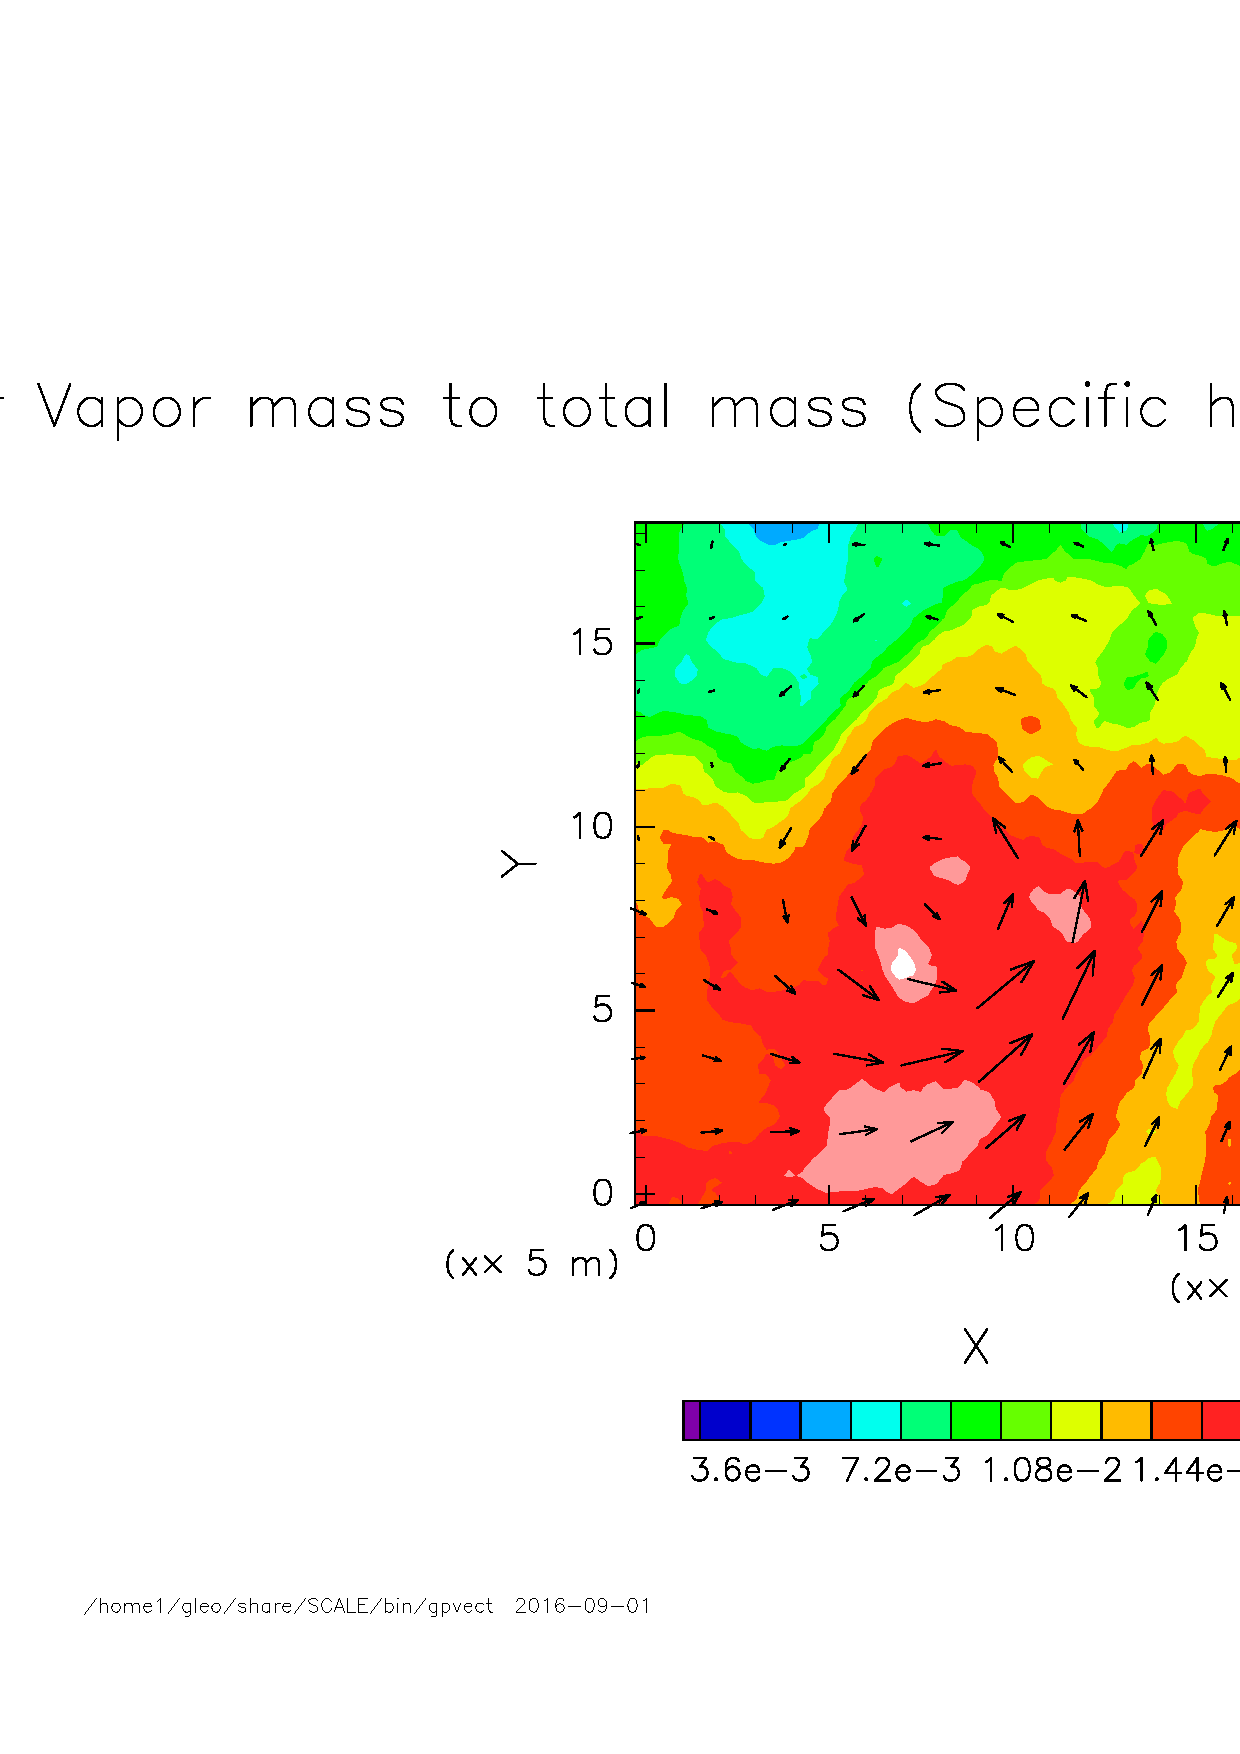
\includegraphics[width=0.9\hsize]{./figure/real_init_qv-momxy.pdf}\\
  \caption{チュートリアル実験における初期場の様子($z=$1500 m)。
           色は比湿、ベクトルは水平運動量フラックスを表す。}
  \label{fig:init}
\end{center}
\end{figure}

%-------------------------------------------------------%
\section{シミュレーションの実行:run} \label{sec:tutorial_real_run}
%-------------------------------------------------------%
\subsubsection{run.confの準備}
\verb|run|ディレクトリへ移動する。
\begin{verbatim}
 $ cd ${Tutorial_DIR}/real/experiment/run
\end{verbatim}
%
このディレクトリの中には、表\ref{tab:grids}に示すチュートリアル用の設定を施した設定ファイルが準備されている。
他に\verb|run.launch.conf|というファイルも存在するが、ここでは使用しない。

モデル本体の実行には、事前に作成した地形データや初期値/境界値データを使用する。
これらのファイルの指定は、\verb|run.d01.conf|における下記の部分で設定している。
\editbox{
\verb|&PARAM_TOPOGRAPHY| \\
\verb|   TOPOGRAPHY_IN_BASENAME = "../pp/topo_d01",| \\
\verb|/| \\
 \\
\verb|&PARAM_LANDUSE| \\
\verb|   LANDUSE_IN_BASENAME  = "../pp/landuse_d01",| \\
\verb|/| \\
 \\
\verb|&PARAM_RESTART| \\
\verb| RESTART_OUTPUT       = .true., |\\
\verb| RESTART_OUT_BASENAME = "restart_d01",|\\
\verb| RESTART_IN_BASENAME  = "../init/init_d01_20070714-180000.000",|\\
\verb|/| \\
 \\
\verb|&PARAM_ATMOS_BOUNDARY| \\
\verb| ATMOS_BOUNDARY_TYPE           = "REAL",                |\\
\verb| ATMOS_BOUNDARY_IN_BASENAME    = "../init/boundary_d01",|\\
\verb| ATMOS_BOUNDARY_USE_DENS       = .true.,     |\\
\verb| ATMOS_BOUNDARY_USE_QHYD       = .false.,    |\\
\verb| ATMOS_BOUNDARY_ALPHAFACT_DENS = 1.0,        |\\
\verb| ATMOS_BOUNDARY_LINEAR_H       = .false.,    |\\
\verb| ATMOS_BOUNDARY_EXP_H          = 2.0,        |\\
\verb|/| \\
}


\verb|run.d01.conf|の中で、時間積分に関する設定は\namelist{PARAM_TIME}で行う。
初期時刻は\nmitem{TIME_STARTDATE}にUTCで指定し、
チュートリアルでは2007年7月14日18時UTCに設定している。
積分時間は\nmitem{TIME_DURATION}で与える。
物理過程に対する時間ステップは、各物理スキームごとに設定できる。

\editboxtwo{
\verb|&PARAM_TIME| & \\
\verb| TIME_STARTDATE         = 2007, 7, 14, 18, 0, 0,| & ← 時間積分を開始する時刻 \\
\verb| TIME_STARTMS           = 0.D0,  | &\\
\verb| TIME_DURATION          = 6.0D0, | & : 積分期間 \\
\verb| TIME_DURATION_UNIT     = "HOUR",| & : \verb|TIME_DURATION|の単位\\
\verb| TIME_DT                = 90.0D0,| & : トレーサー移流計算の時間ステップ\\
\verb| TIME_DT_UNIT           = "SEC", | & : \verb|TIME_DT|の単位\\
\verb| TIME_DT_ATMOS_DYN      = 45.0D0,| & : トレーサー移流計算以外の力学過程の時間ステップ\\
\verb| TIME_DT_ATMOS_DYN_UNIT = "SEC", | & : \verb|TIME_DT_ATMOS_DYN|の単位\\
 \\
\verb|   ..... 略 .....              | & \\
 \\
\verb|/| &\\
}

計算結果の出力に関する設定は、\nmitem{PARAM_FILE_HISTORY}で行う。

\editboxtwo{
\verb|&PARAM_FILE_HISTORY| & \\
\verb|   FILE_HISTORY_DEFAULT_BASENAME  = "history_d01",| & : 出力するファイル名\\
\verb|   FILE_HISTORY_DEFAULT_TINTERVAL = 3600.D0,      | & : 出力時間間隔\\
\verb|   FILE_HISTORY_DEFAULT_TUNIT     = "SEC",        | & : 出力時間間隔の単位\\
\verb|   FILE_HISTORY_DEFAULT_TAVERAGE  = .false.,      | & \\
\verb|   FILE_HISTORY_DEFAULT_DATATYPE  = "REAL4",      | & \\
\verb|   FILE_HISTORY_DEFAULT_ZCOORD    = "model",      | & : 鉛直内挿は適用しない\\
\verb|   FILE_HISTORY_OUTPUT_STEP0      = .true.,       | & : 初期時刻(t=0)の値を出力するかどうか\\
\verb|/| \\
}

上記の設定に従って、下記の\nmitem{HISTOTRY_ITEM}に列挙した変数を出力する。
必要があれば、\nmitem{HISTOTRY_ITEM}においてオプション変数を加えることで、変数毎に出力間隔を変更できる。
また、瞬間値の代わりに平均値を出力することも可能である。
これらの詳細は、\ref{sec:output}を参照されたい。

\editboxtwo{
\verb|&HISTOTRY_ITEM name="MSLP" /|        & 海面更正気圧 \\
\verb|&HISTOTRY_ITEM name="PREC" /|        & 降水強度 (2次元) \\
\verb|&HISTOTRY_ITEM name="OLR"  /|        & 外向き赤外放射(2次元) \\
\verb|&HISTOTRY_ITEM name="U10m" /|        & 地表10mでの東西方向水平速度成分(2次元) \\
\verb|&HISTOTRY_ITEM name="V10m" /|        & 地表10mでの南北方向水平速度成分(2次元) \\
\verb|&HISTOTRY_ITEM name="U10" / |        & 地表10mでのX方向水平速度成分(2次元) \\
\verb|&HISTOTRY_ITEM name="V10" / |        & 地表10mでのY方向水平速度成分(2次元) \\
\verb|&HISTOTRY_ITEM name="T2"  / |        & 地表2mでの温度 (2次元) \\
\verb|&HISTOTRY_ITEM name="Q2"  / |        & 地表2mでの水蒸気比湿 (2次元) \\
\verb|&HISTOTRY_ITEM name="SFC_PRES"   /|   & 地表気圧 (2次元) \\
\verb|&HISTOTRY_ITEM name="SFC_TEMP"   /|   & バルクの地表面温度 (2次元) \\
\verb|&HISTOTRY_ITEM name="DENS" /|        & 密度 (3次元) \\
\verb|&HISTOTRY_ITEM name="QV"   /|        & 水蒸気比湿 (3次元) \\
\verb|&HISTOTRY_ITEM name="QHYD" /|        & 全凝結物の全質量に対する比 (3次元) \\
\verb|&HISTOTRY_ITEM name="PRES" /|        & 気圧 (3次元) \\
\verb|&HISTOTRY_ITEM name="Umet" /|        & 東西方向水平速度成分 (3次元) \\
\verb|&HISTOTRY_ITEM name="Vmet" /|        & 南北方向水平速度成分 (3次元) \\
\verb|&HISTOTRY_ITEM name="U"    /|        & X方向水平速度成分 (3次元) \\
\verb|&HISTOTRY_ITEM name="V"    /|        & Y方向水平速度成分 (3次元) \\
\verb|&HISTOTRY_ITEM name="T"    /|        & 温度 (3次元) \\
\verb|&HISTOTRY_ITEM name="W"    /|        & 鉛直方向速度成分 (3次元) \\
\verb|&HISTOTRY_ITEM name="Uabs" /|        & 風速 (3次元) \\
\verb|&HISTOTRY_ITEM name="PT"   /|        & 温位 (3次元) \\
\verb|&HISTOTRY_ITEM name="RH"   /|        & 相対湿度 (3次元) \\
}

力学過程や物理過程に対するスキームとして他のスキームを用いたい場合は、
力学過程に関しては\namelist{&PARAM_ATMOS_DYN}、
物理過程に関しては\namelist{PARAM_ATMOS,PARAM_OCEAN,PARAM_LAND,PARAM_URBAN}で設定できる。
詳細は、第\ref{sec:atmos_dyn_cartesC}節、\ref{sec:basic_usel_physics}節を参照されたい。

%
\subsubsection{シミュレーションの実行}

実行に必要なファイルは下記であり、あらかじめ用意されている。
\begin{alltt}
 $ ls
    MIPAS  PARAG.29  PARAPC.29  VARDATA.RM29  cira.nc
                                  : 放射スキーム用のパラメータファイル
    run.d01.conf      : 設定ファイル
    param.bucket.conf : 陸面スキーム用のパラメータファイル
    scale-rm          : \scalerm の実行バイナリ
    run.launch.conf   : ネスティング計算用のlaunchファイル
                       (チュートリアルでは使用しない)
\end{alltt}
%
準備が整ったら、4-MPI 並列により\scalerm を実行する。
\begin{verbatim}
  $ mpirun -n 4 ./scale-rm run.d01.conf >& log &
\end{verbatim}


実行が完了するまでには、ある程度時間を要する(推奨環境において10〜20分程度かかる)。
そのため、上記のように標準出力をファイルに書き出すようにして、
バックグラウンドで実行すると便利である。
計算は進みながら、途中経過のログは\verb|"LOG_d01.pe000000"|に出力される。
ジョブが正常に終了すると、\verb|"LOG_d01.pe000000"|の最後に
\msgbox{
 +++++ finalize MPI...\\
 +++++ MPI is peacefully finalized\\
}
と出力され、下記のファイルが作成される。
\begin{verbatim}
 $ ls
  history_d01.pe000000.nc
  history_d01.pe000001.nc
  history_d01.pe000002.nc
  history_d01.pe000003.nc
\end{verbatim}
各ファイルのサイズは約 34 MB である。
出力ファイル(\verb|history_d01.pe######.nc|)は、MPI プロセス数に応じて分割されている。
ここで、\verb|######|はMPIプロセス番号を表す。
これらのファイルには、\nmitem{HISTORY_ITEM}で指定した変数が出力されている。
出力ファイルの形式は、気候・予報(CF)メタデータ規約に準拠した NetCDF である。


%####################################################################################

\section{結果のクイック描画:net2g} \label{sec:quicklook}
%####################################################################################

本節では、\verb|netcdf2grads|の使用方法を説明する。
プログラム\verb|netcdf2grads| (略して \verb|net2g|)は、プロセス毎に分割された{\netcdf}ファイル(\verb|history.**.nc|
\footnote{「gpview」がインストールされている場合には、「gpview」でも作図することができる。
このツールは historyデータを変換することなく直接作図することができるため、
素早く結果を確認した場合には適している。
}
)
を{\grads}形式の単一のバイナリファイルに結合する。
この変換した{\grads}バイナリデータを使って、シミュレーションの結果を確認する。


\subsubsection{{\grads}バイナリに変換}
%-----------------------------------------------------------------------------------
プロセスごとに分割された{\netcdf}形式のヒストリファイルから{\grads}バイナリに変換するために、\verb|net2g|を使用する。
ここでは最低限の手順のみを説明することにする。
詳細な使用方法は\ref{sec:net2g}節を参照されたい。

まず、\verb|net2g|ディレクトリに移動する。
\begin{verbatim}
 $ cd ${Tutorial_DIR}/real/experiment/net2g
 $ ls
    Makefile
    net2g -> ../../../../../util/netcdf2grads_h/net2g
    net2g.2D.d01.conf
    net2g.3D.d01.conf
\end{verbatim}
このディレクリの中には設定ファイルとバイナリファイルがある。
バイナリファイルは、\ref{sec:source_net2g}節でコンパイルした実行ファイルにリンクされている。
ここでは例として、2次元変数のMSLP、PRECを{\grads}形式に変換する手順を示す。
また、3次元変数の 東西風(Umet)、南北風(Vmet)を 850 hPa 面、500hPa 面、200 hPa 面で抽出して、
{\grads}形式に変換する手順も説明する。
2次元変数と3次元変数のための設定ファイルはそれぞれ、
\verb|net2g.2D.d01.conf| と \verb|net2g.3D.d01.conf| である。

\verb|net2g|を実行する時のプロセス数は、
シミュレーションの実行時に用いたプロセス数の約数である必要がある。
ここでは、4プロセスを使用する。
net2g は2次元変数と3次元変数を同時に変換できないために、
以下のように別々に実行する。
\begin{verbatim}
 $ mpirun -n 4 ./net2g net2g.2D.d01.conf
 $ mpirun -n 4 ./net2g net2g.3D.d01.conf
\end{verbatim}
エラーメッセージがなく、下記のメッセージだけが標準出力へ表示されていれば、
変換は正常に完了している。\\

\noindent {\gt
\fbox{
\begin{tabularx}{150mm}{l}
\verb|+++ MPI COMM: Corrective Finalize| \\
\end{tabularx}
}}\\

成功すれば、下記のファイルが作成される。
\verb|**.ctl|は {\scalerm} のXY格子系に対するctlファイル、
\verb|**lccr.ctl|は緯度経度座標系で結果を作図するためのctlファイルである。

\begin{verbatim}
  MSLP_d01z-2d.ctl
  MSLP_d01z-2d.grd
  MSLP_d01z-2d_lccr.ctl
  PREC_d01z-2d.ctl
  PREC_d01z-2d.grd
  PREC_d01z-2d_lccr.ctl
  PRES_d01z-3d.ctl
  PRES_d01z-3d.grd
  PRES_d01z-3d_lccr.ctl
  Umet_d01z-3d.ctl
  Umet_d01z-3d.grd
  Umet_d01z-3d_lccr.ctl
  Vmet_d01z-3d.ctl
  Vmet_d01z-3d.grd
  Vmet_d01z-3d_lccr.ctl
\end{verbatim}




\subsubsection{計算結果の確認}
%-----------------------------------------------------------------------------------

%\verb|${Tutorial_DIR}/real/data|ディレクトリに用意してあるので、
%サンプルとして利用してほしい。\footnote{今後、緯度経度座標で描画するためのctlファイルを出力できるようにする予定。}
%\begin{verbatim}
% $ cp ../../data/*_lcc.ctl ./
% $ ls
%    MSLP_d01z-2d_lcc.ctl
%    PREC_d01z-2d_lcc.ctl
%    U_d01z-3d_lcc.ctl
%    V_d01z-3d_lcc.ctl
%\end{verbatim}

\grads スクリプト\verb|checkfig_real.gs|を用いて、計算結果を確認する。
\begin{verbatim}
 $ cp ../../data/checkfig_real.gs ./
 $ grads -blc checkfig_real.gs
\end{verbatim}
変換が正常に終了すれば、下記のファイルが作成される。
なお、\grads のバージョンによって文法が異なるので、警告が出る場合はスクリプトを適宜変更されたい。
\begin{verbatim}
  real_mslp.png
  real_prec.png
  real_wind.png
\end{verbatim}
計算が成功していれば、
図\ref{fig:real_mslp}, \ref{fig:real_prec}, \ref{fig:real_wind}と同じ図が得られる。


\begin{figure}[h]
\begin{center}
  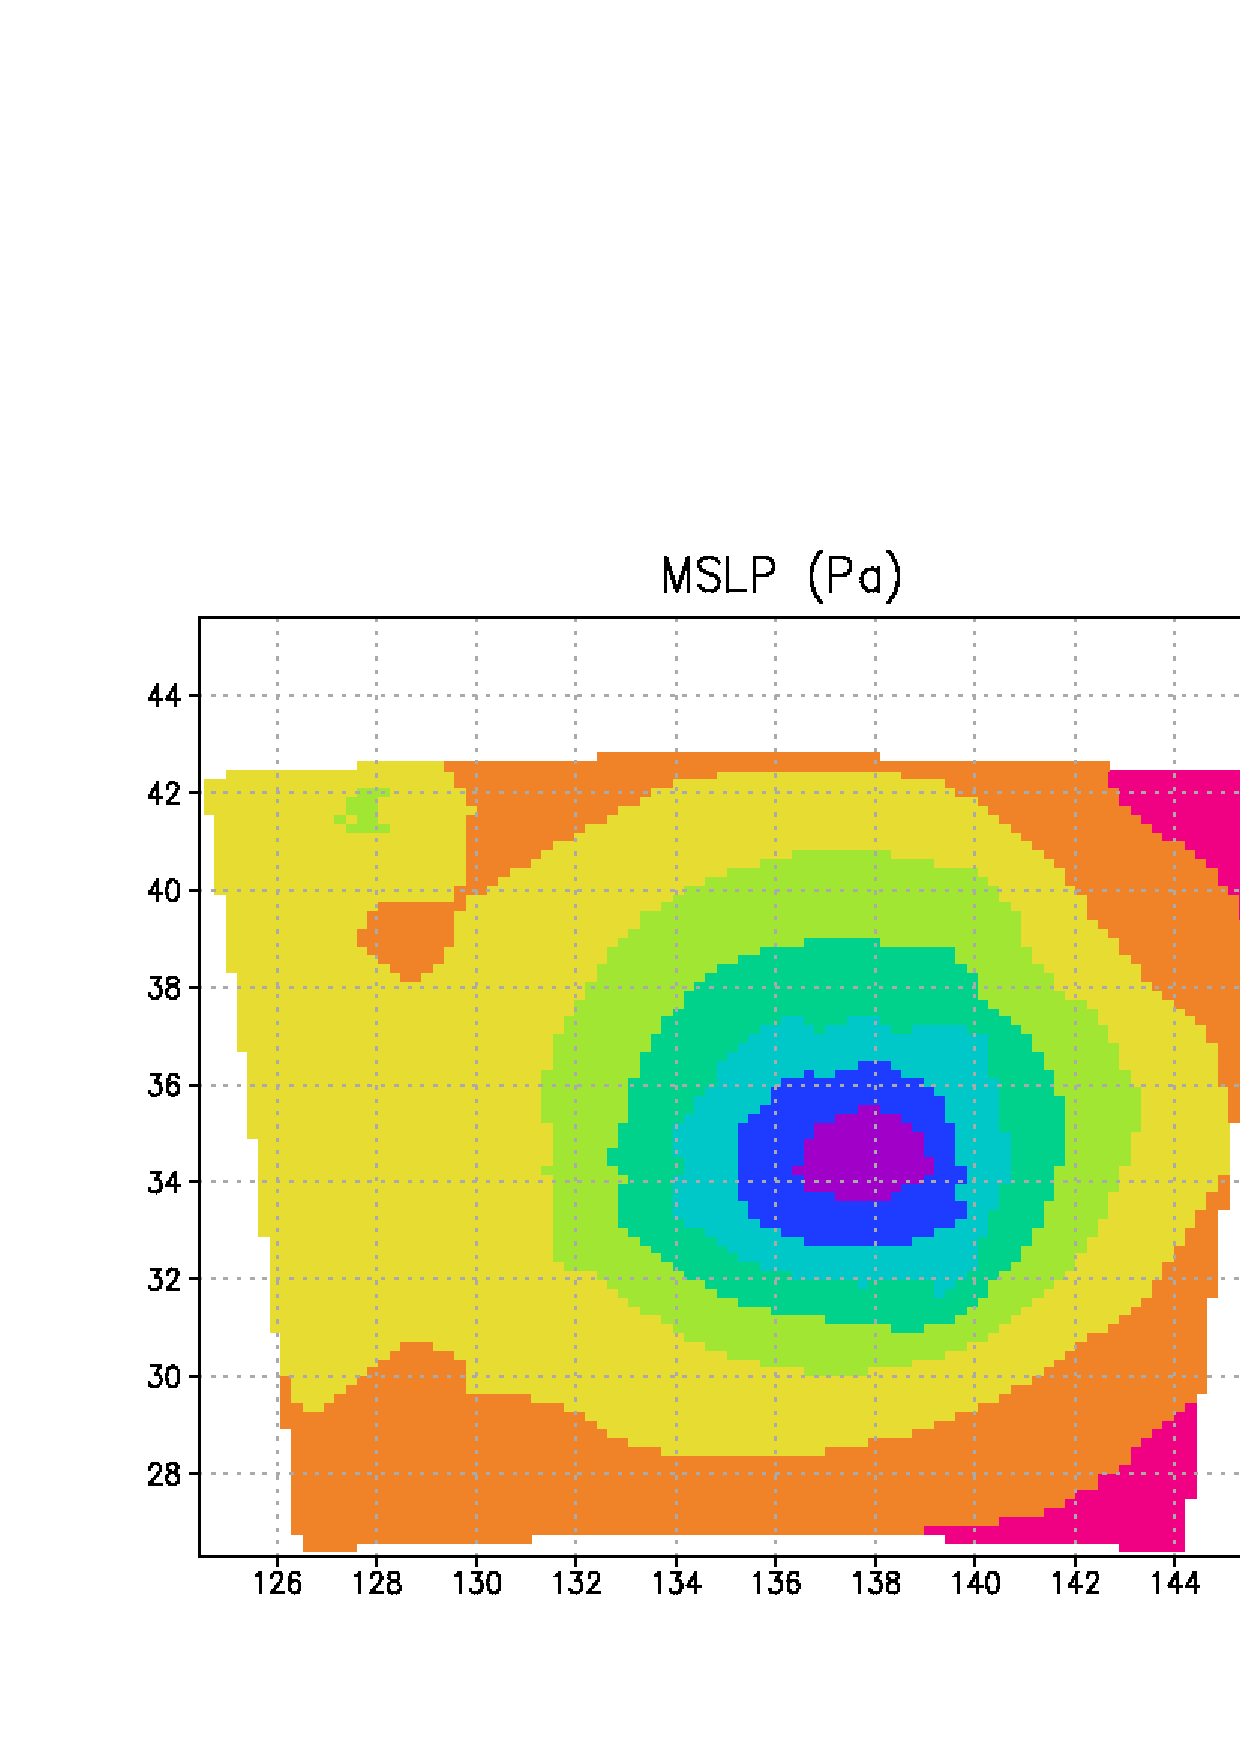
\includegraphics[width=0.55\hsize]{./figure/real_mslp.pdf}\\
  \caption{計算開始から6時間後の海面更正気圧}
  \label{fig:real_mslp}
\end{center}
\begin{center}
  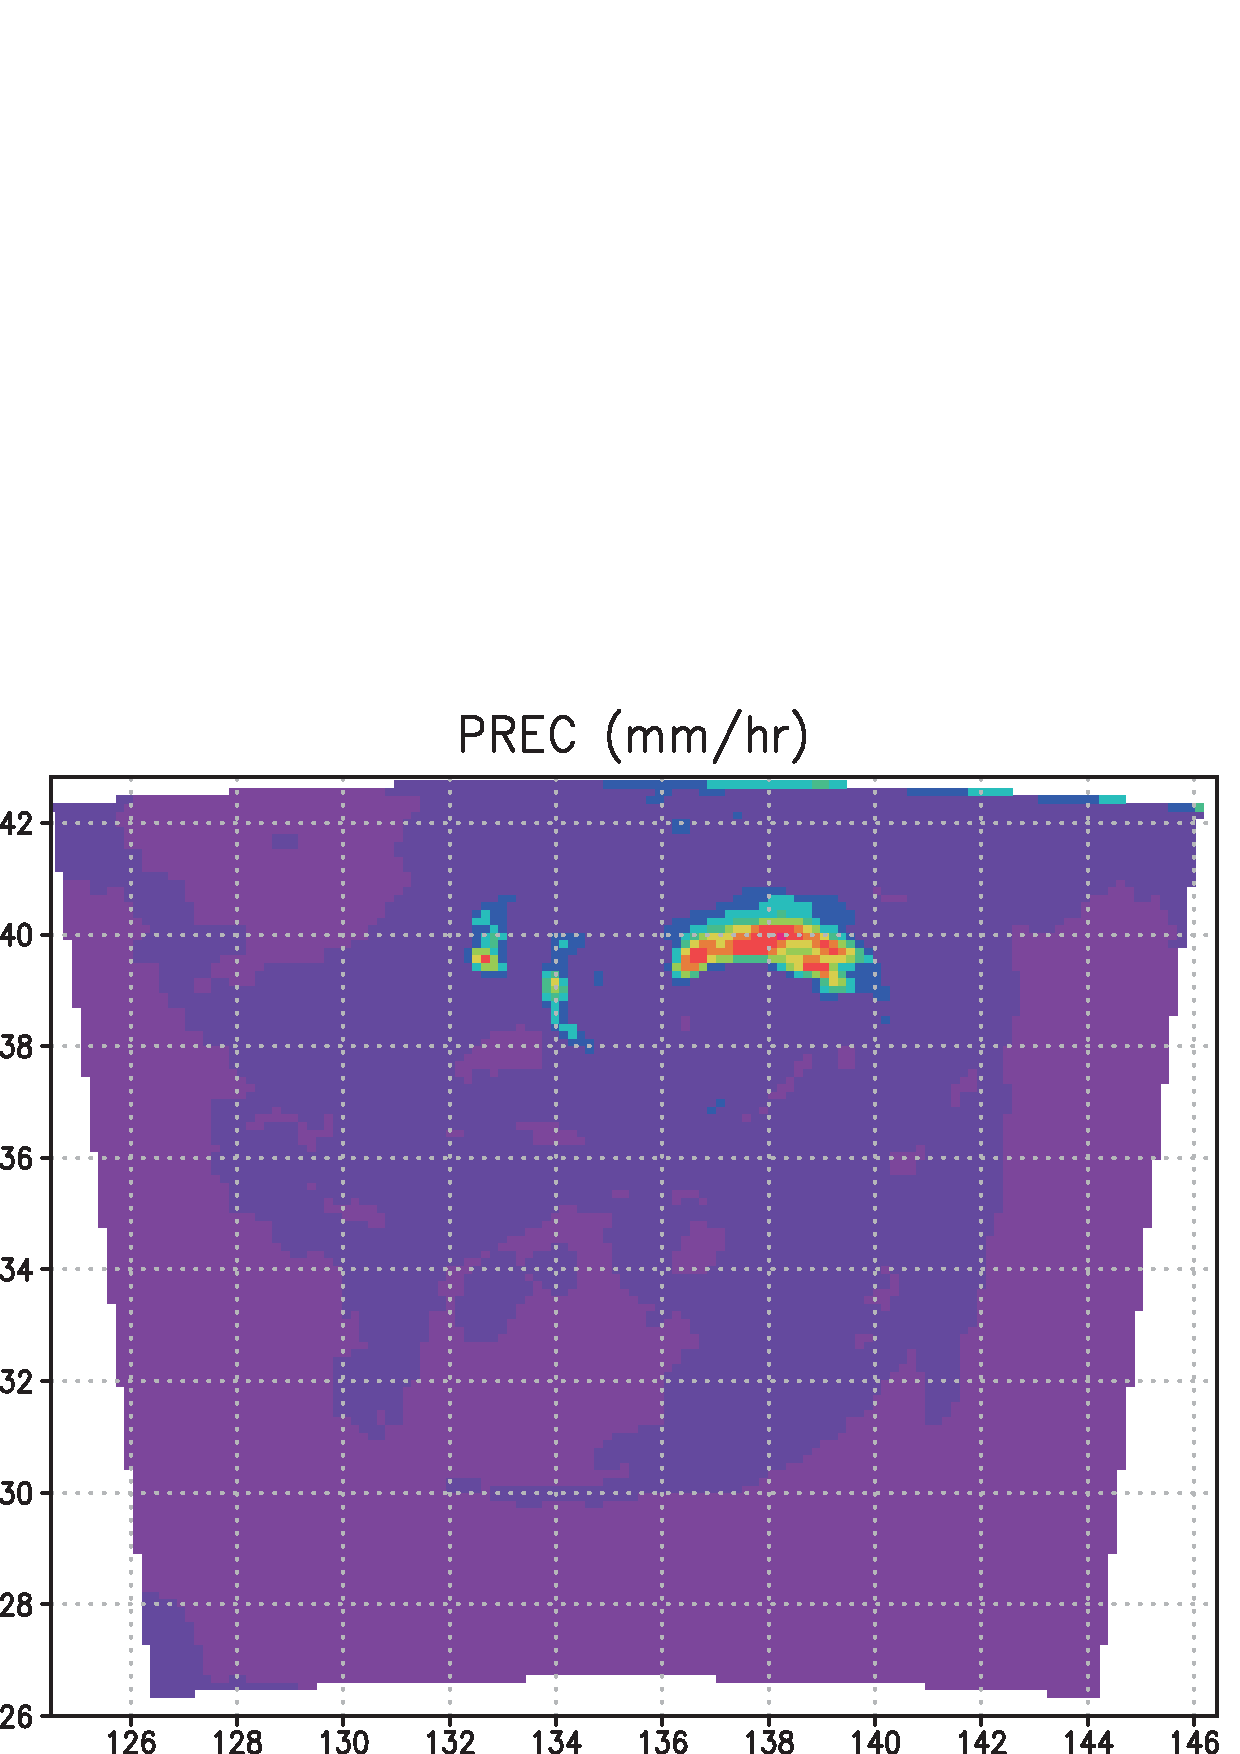
\includegraphics[width=0.55\hsize]{./figure/real_prec.pdf}\\
  \caption{計算開始から6時間後の降水フラックス}
  \label{fig:real_prec}
\end{center}
\begin{center}
  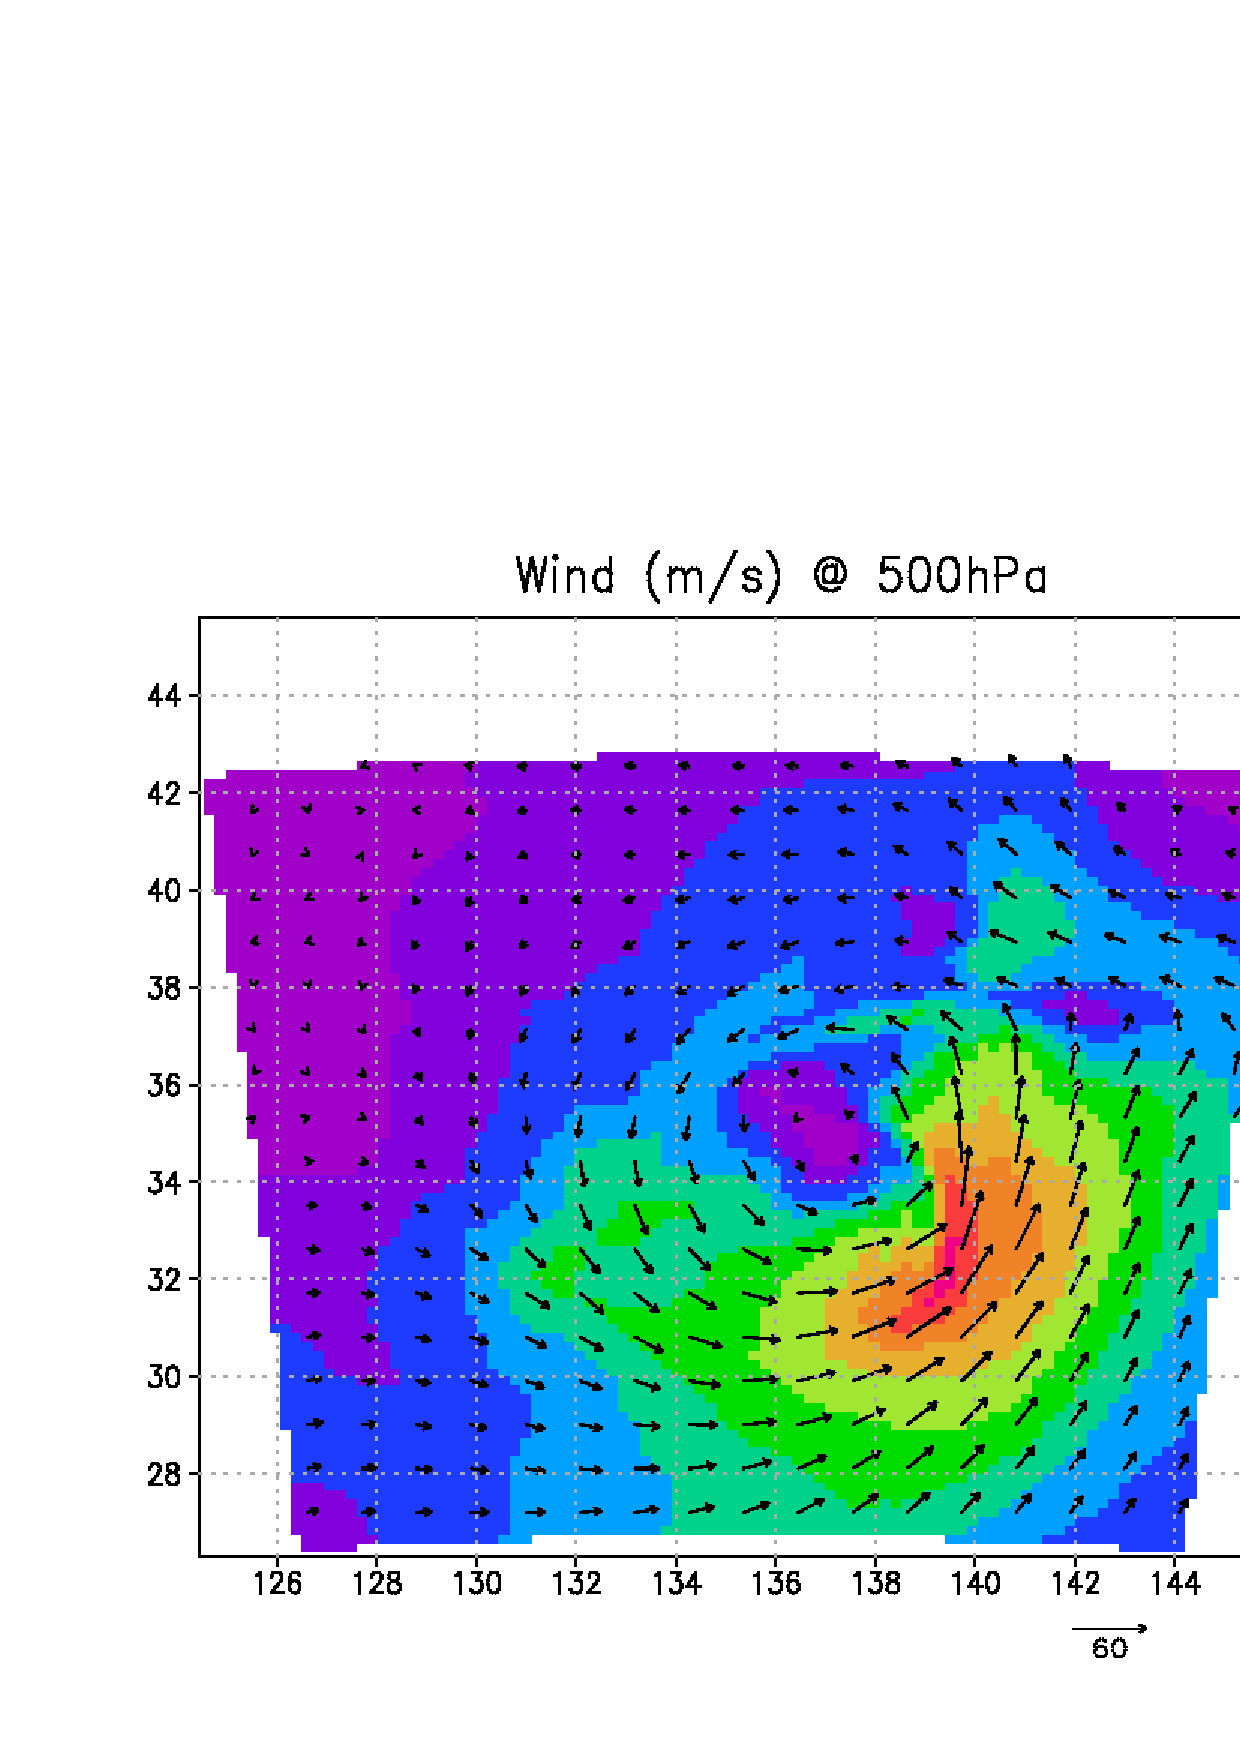
\includegraphics[width=0.55\hsize]{./figure/real_wind.pdf}\\
  \caption{計算開始から6時間後の850hPaの風速(色は絶対値、ベクトルは向き)}
  \label{fig:real_wind}
\end{center}
\end{figure}


\chapter{各種設定} \label{chap:basic_usel}
%\section*{概要}

この章では、チュートリアルから発展して、基本的な様々な設定が出きるように、
各種設定を網羅的に記述している。
各節で閉じており、辞書代わりに使ってほしい。

%% {
%% \begin{center}
%% \begin{tabular}[h]{ll}\hline
%% \SecBasicDomainSetting & 第\ref{sec:domain} 節 \\
%%%%%% \SubsecDomainSetting & 第\ref{subsec:relation_dom_reso2} 節 \\
%% \SubsecMPIProcess & 第\ref{subsec:relation_dom_reso2} 節 \\
%% \SubsecGridNumSettng & 第\ref{subsec:relation_dom_reso3} 節 \\
%% \SubsecGridIntvSettng & 第\ref{subsec:gridinterv} 節 \\
%% \SecBasicBufferSetting & 第\ref{subsec:buffer} 節 \\
%% \SecBasicTopoSetting   & 第\ref{subsec:basic_usel_topo} 節 \\
%% \SecBasicIntegrationSetting & 第\ref{sec:timeintiv} 節 \\
%% \SecBasicOutputSetting & 第\ref{sec:output} 節\\
%% \SecBasicDynamicsSetting & 第\ref{sec:atmos_dyn} 節 \\
%% \SubsecDynsolverSetting  & 第\ref{subsec:atmos_dyn_sover} 節 \\
%% \SubsecDynSchemeSetting & 第\ref{subsec:atmos_dyn_scheme} 節 \\
%% \SecBasicPhysicsSetting & 第\ref{sec:basic_usel_physics} 節 \\
%% \SubsecMicrophysicsSetting & 第\ref{subsec:basic_usel_microphys} 節 \\
%% \SubsecTurbulenceSetting & 第\ref{subsec:basic_usel_turbulence} 節 \\
%% \SubsecRadiationSetting & 第\ref{subsec:basic_usel_radiation} 節 \\
%% \SubsecSurfaceSetting & 第\ref{subsec:basic_usel_surface} 節 \\
%% \SubsecOceanSetting & 第\ref{subsecp:basic_usel_ocean} 節 \\
%% \SubsecLandSetting & 第\ref{subsec:basic_usel_land} 節 \\
%% \SubsecUrbanSetting & 第\ref{subsec:basic_usel_urban} 節 \\
%% \SecMakeconfTool & 第\ref{sec:basic_makeconf} 節 \\
%% \SecAdvanceMapprojectionSetting & 第\ref{subsec:adv_mapproj}節 \\
%% \SecAdvanceInputDataSetting & 第\ref{sec:adv_datainput}節\\
%% \SecAdvanceRestart & 第\ref{sec:restart}節 \\
%% \SecAdvancePostprosess & 第\ref{sec:net2g}節 \\
%% \SecAdvanceNesting & 第\ref{sec:nest_exp}節 \\
%% \SubsecOflineNesting & 第\ref{subsec:nest_offline}節\\
%% \SubsecOnlineNesting & 第\ref{subsec:nest_online}節\\
%% \SecAdvanceBulkjob & 第\ref{sec:bulkjob}節\\
%% \hline
%% \end{tabular}
%% \end{center}
%% }

\section{Setting the target domain} \label{sec:domain}
%=======================================================================

This section explains the number of grids, and the target domain and its relationship with the MPI process. The calculation domain is determined by the horizontal grid spacing, the number of grid points, and the number of MPI processes. Figure \ref{fig:domain} gives an example of this relationship. The parallelization is implemented by a 2D domain decomposition in the horizontal direction.

The numbers of grids and of MPI processes are specified in \nmitem{IMAX, JMAX} in\\
\namelist{PARAM_ATMOS_GRID_CARTESC_INDEX}, and in \nmitem{PRC_NUM_X, PRC_NUM_Y} in \namelist{PARAM_PRC_CARTESC}, respectively. As shown in Fig. \ref{fig:domain},  the entire domain is divided into \nmitem{PRC_NUM_X} along the X direction and \nmitem{PRC_NUM_Y} in the Y direction.
The process number starts zero and is numbered in order from the bottom left to the top right (Arrow in Fig. \ref{fig:domain}).
Each sub-domain is managed by an MPI process, each of which takes charge of a grid block of IMAX $\times$ JMAX $\times$ KMAX. Care is taken to ensure that this number of grids is taken charge of by one process: its value is not identical to the total number of grids in the domain. In other words, the entire domain depends on the number of MPI processes, the horizontal grid spacing, and the number of grids.

Thus, the number of grids along each horizontal direction and that in the entire domain are derived as follows:
\begin{eqnarray}
&& \verb|Number of grids in the X direction| = \verb|IMAX| \times \verb|PRC_NUM_X|
   \label{eq:xgridnum}\\
&& \verb|Number of grids in the Y direction| = \verb|JMAX| \times \verb|PRC_NUM_Y|
   \label{eq:ygridnum}\\
&& \verb|Total number of grids in the domain| \nonumber\\
&&\quad = \left(\verb|IMAX| \times \verb|PRC_NUM_X|\right)
          \times (\verb|JMAX| \times \verb|PRC_NUM_Y|)
          \times (\verb|KMAX| ),
\end{eqnarray}
where \nmitem{KMAX} is the number of grids along the vertical direction, which is specified in\\
\namelist{PARAM_ATMOS_GRID_CARTESC_INDEX}.

By using Eqs. (\ref{eq:xgridnum} and \ref{eq:ygridnum}),  the size of the entire domain is determined as follows:
\begin{eqnarray}
&& \verb|Domain length in the X direction| \nonumber\\
&&    \qquad = \verb|number of grids in the X direction| \times \verb|DX|\\
&& \verb|Domain length in the Y direction| \nonumber\\
&&    \qquad = \verb|number of grids in the Y direction| \times \verb|DY|,
\end{eqnarray}
where \nmitem{DX, DY} is grid spacings specified  in \namelist{PARAM_ATMOS_GRID_CARTESC} as described in subsection \ref{subsec:gridinterv}.
If the horizontal resolution and domain size are set and the available number of MPI processes is given, the number of grids that are controlled by one MPI process can be determined as in the above relationship.

In order to perform a horizontal-vertical two-dimentional experiment, set both the \texttt{IMAX} and \texttt{PRC\_NUM\_X} to 1, i.e., the total number of the grids in the X direction is one.
In this case, the motion in the Y-Z section is calculated.
The value of \texttt{DX} does not affect the simulation result.

In the next subsections, the configuration of the MPI processes, the number of grids, and the grid interval are described in more detail.  \textcolor{blue}{Note that it is necessary that these settings  be identical among the configuration files \texttt{pp.conf},  \texttt{init.conf}, and \texttt{run.conf}}.

\begin{figure}[h]
\begin{center}
  \includegraphics[width=0.8\hsize]{./figure/domain_decomposition_v2.png}\\
  \caption{Relation between horizontal grid interval (\texttt{DX}, \texttt{DY}),
   number of grids (\texttt{IMAX}, \texttt{JMAX}) per MPI process,
   and the number of MPI processes (\texttt{PRC\_NUM\_X}, \texttt{PRC\_NUM\_Y}) in the entire domain.
   The light-blue part corresponds to a region managed by an MPI process.
   The six digit number following ``pe'' shows the process number.}
  \label{fig:domain}
\end{center}
\end{figure}

%-----------------------------------------------------------------------
\subsection{Setting the number of MPI processes} \label{subsec:relation_dom_reso2}
%-----------------------------------------------------------------------

The number of MPI processes is specified in \namelist{PARAM_PRC_CARTESC} in the configuration file. Since the input and output files of \scalerm are divided process by process according to the MPI, the total number of files is changed according to the number of MPI processes. For example, the initial condition file made by a two-MPI parallel combination cannot be used for model execution by a four-MPI parallel.
It is necessary to edit \namelist{PARAM_PRC_CARTESC} in \verb|pp.conf|, \verb|init.conf|, and \verb|run.conf| if the number of MPI processes is changed,
and to conduct once again the processes of \verb|pp| and \verb|init|.
\editboxtwo{
\verb|&PARAM_PRC_CARTESC| & \\
\verb| PRC_NUM_X       = 2,| & ; number of divisions by MPI parallelization in the {\XDIR} (zonal direction) \\
\verb| PRC_NUM_Y       = 1,| & ; number of divisions by MPI parallelization in the {\YDIR} (meridional direction) \\
\verb|/|\\
}
The total number of MPI processes is given by \verb|PRC_NUM_X| $\times$ \verb|PRC_NUM_Y|.
The above example expresses a two-MPI parallel by dividing the domain into two sub-domains along the X direction, but not dividing along the Y direction. The total number of processes must be given as the number of MPI processes in the MPI command at submitting job. If this condition is not satisfied,  the program is terminated immediately without calculation and the following message is output to the standard output.
\msgbox{
\verb|xxx total number of node does not match that requested. Check!| \\
}

%-----------------------------------------------------------------------
\subsection{Setting the number of horizontal and vertical grids} \label{subsec:relation_dom_reso3}
%-----------------------------------------------------------------------

The number of grids is specified in \namelist{PARAM_ATMOS_GRID_CARTESC_INDEX} in the configuration files \verb|***.conf|. It should be noted that the specified horizontal grids are values controlled by one MPI process.
\editboxtwo{
\verb|&PARAM_ATMOS_GRID_CARTESC_INDEX| & \\
\verb| KMAX = 97,|  & ; number of vertical layers \\
\verb| IMAX = 20,|  & ; number of grids along the X direction by an MPI process\\
\verb| JMAX = 25,|  & ; number of grids along the Y direction by an MPI process\\
\verb|/|\\
}

%-----------------------------------------------------------------------
\subsection{Setting grid intervals along the horizontal and vertical directions} \label{subsec:gridinterv}
%-----------------------------------------------------------------------

Excluding the buffer region explained in Section \ref{subsec:buffer}, the horizontal grid intervals are configured only equidistantly, whereas the
 vertical grid intervals are configured freely. When the grid intervals are  configured uniformly along all directions, specify the zonal, meridional, and vertical grid intervals  at \nmitem{DX, DY, DZ} in \namelist{PARAM_ATMOS_GRID_CARTESC}, respectively. The unit is [m].
\editboxtwo{
\verb|&PARAM_ATMOS_GRID_CARTESC  | & \\
\verb| DX = 500.D0,| & ; grid interval along the zonal (X) direction\\
\verb| DY = 500.D0,| & ; grid interval along the meridional (Y) direction\\
\verb| DZ = 500.D0,| & ; grid interval along the vertical (Z) direction\\
\verb|/|\\
}

The box below shows the method to set how to specify a non-uniform grid system.
Since the model employs the Lorenz grid system, the points of definition for the velocity vector and other scalars are staggered, deviating by a half grid.
In this document, the scalar location is called the center point and the half-grid-deviated location the face point.
When the vertical grid locations are directly specified, provide them in \nmitem{FZ(:)} in \namelist{PARAM_ATMOS_GRID_CARTESC} as an array.\footnote{In this case, the same precision as used in the simulation is recommended to be specified. By default, the model is compiled as a double-precision floating point model.} Refer to Figure \ref{fig:scale_grid} for the details. Note that the number of elements specified in \nmitem{FZ(:)} should correspond to the number of vertical layers (\nmitem{KMAX} in \namelist{PARAM_ATMOS_GRID_CARTESC_INDEX}). The following file for the ideal experiment is shown as an example:
\editboxtwo{
\verb|&PARAM_ATMOS_GRID_CARTESC|     & \\
\verb| DX = 500.D0,|   & grid interval along the X direction (equidistant) [m]\\
\verb| DY = 500.D0,|   & grid interval along the Y direction (equidistant) [m]\\
\verb| FZ(:) = |       & location at face point along the Z direction [m] \\
\verb|     80.000000000000000      ,| & \\
\verb|     168.00000190734863      ,| & \\
\verb|     264.80000610351567      ,| & \\
\verb|           ........           | & \\
\verb|     14910.428862936289      ,| & \\
\verb|     15517.262523292475      ,| & \\
\verb|     16215.121232702089      ,| & \\
\verb|     17017.658748523147      ,| & \\
\verb|     17940.576891717363      ,| & \\
\verb|     19001.932756390710      ,| & \\
\verb|     20222.492000765058      ,| & \\
\verb| BUFFER_DZ = 5000.D0,|          & Refer to Section \ref{subsec:buffer}\\
\verb| BUFFFACT  =   1.0D0,|          & Refer to Section \ref{subsec:buffer}\\
\verb|/|\\
}

\begin{figure}[tb]
\begin{center}
  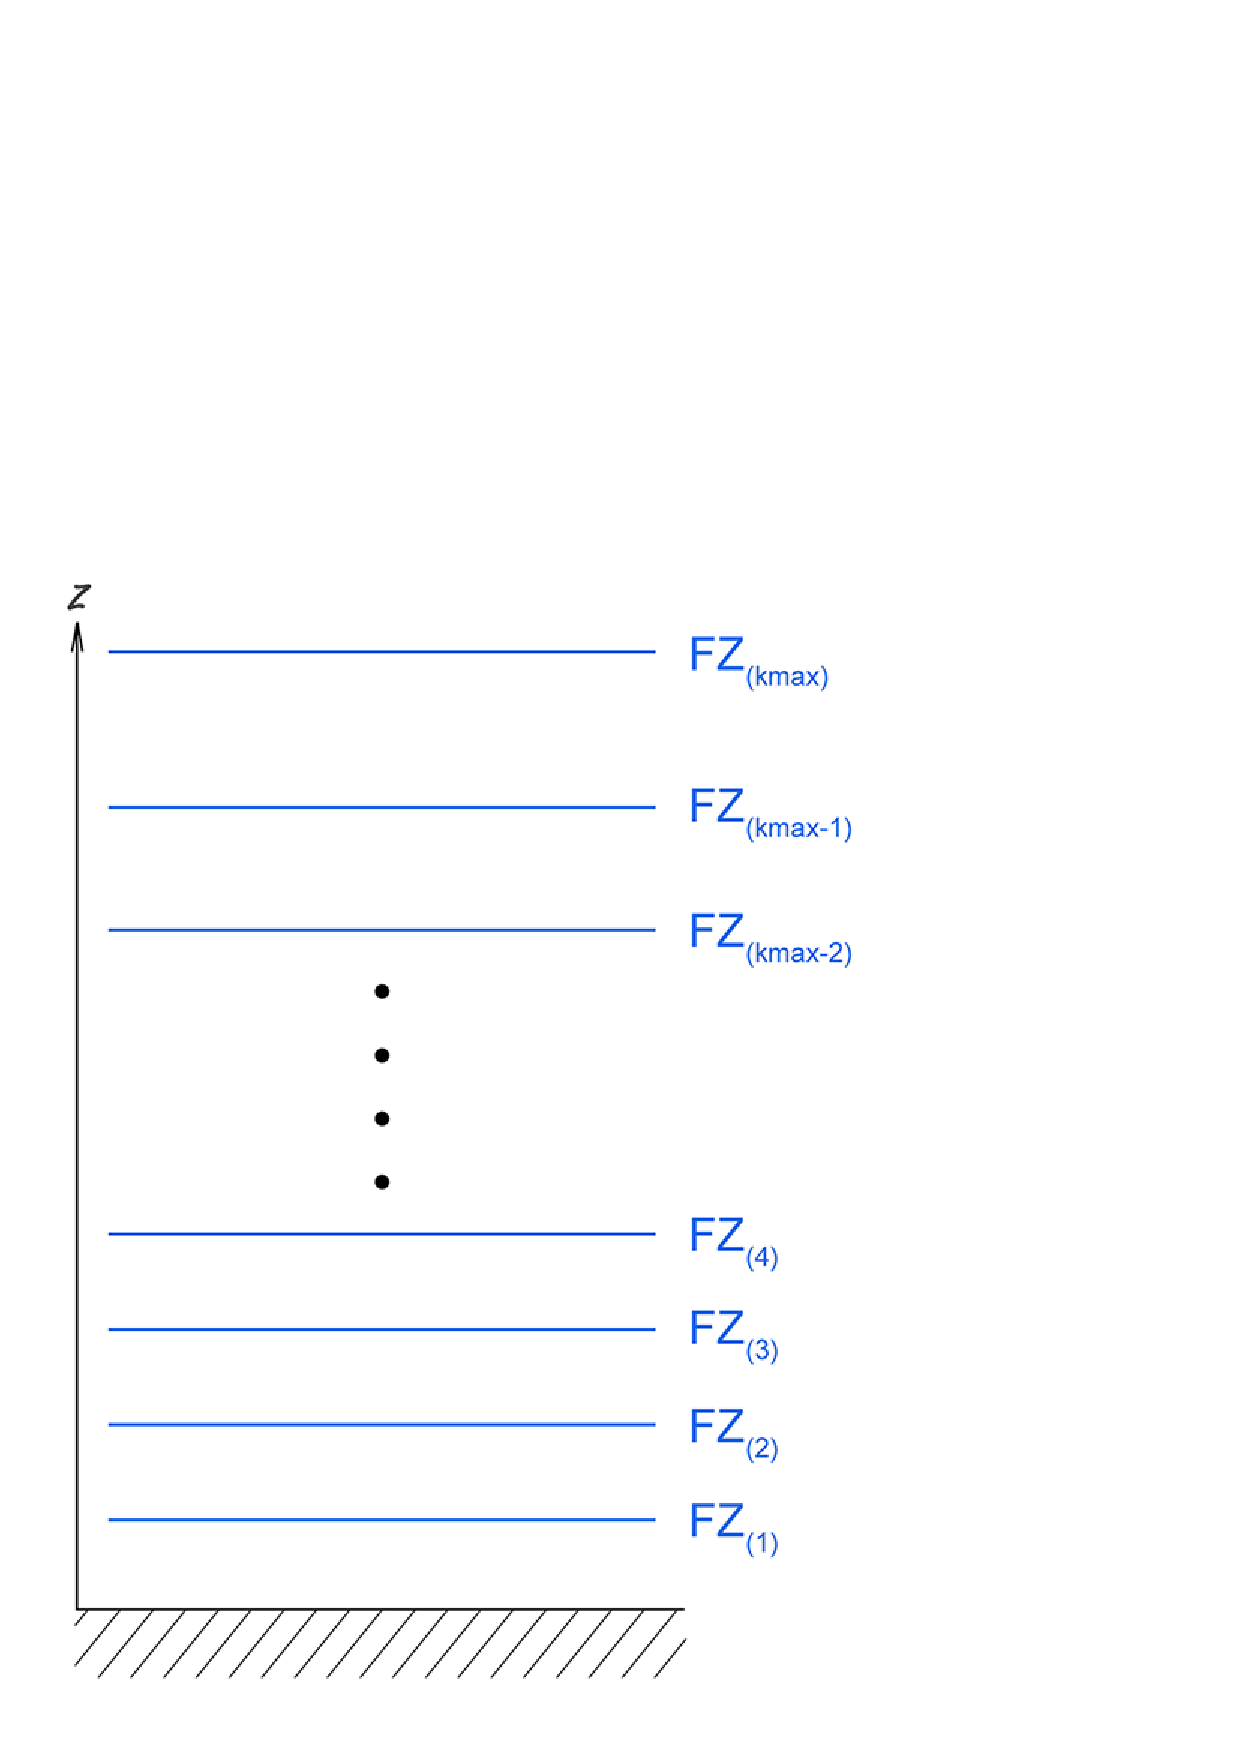
\includegraphics[width=0.4\hsize]{./figure/verticalface.pdf}\\
  \caption{The point of definition of the face point in \scalerm. If \nmitem{FZ} is given in \namelist{PARAM_ATMOS_GRID_CARTESC}, the top height at the first layer is given for the value at $k=1$. Note that $k=1$ is not the ground surface height.}
  \label{fig:scale_grid}
\end{center}
\end{figure}

The above setting is processed at a topographical height of 0 m.
The location of the vertical grids at the non-zero topography is appropriately treated by the terrain-following coordinate.

The locations of the vertical grids are configured freely.
However, an unusual configuration sometimes leads to numerical instability. To avoid it, the tool for the generation of vertical grids is supported as a FORTRAN program \verb|make_vgrid.f90| in the directory\\ \texttt{scale-\version/scale-rm/util/makevgrid/} with several samples of the namelist. If needed, use them as references. The tool generates the values of \nmitem{FZ(:)} directly. Copy and paste them in the configuration file.

%-----------------------------------------------------------------------
\subsection{Setting sponge layer} \label{subsec:raydamp}
%-----------------------------------------------------------------------

\scalerm adopts height coordinate system in vertical. The uppermost boundary condition is a rigid lid, and the sound and gravity waves often reflect at the model top. To reduce worse effects of these reflecting waves, the damping layer named ``sponge layer'' is placed in the upper part of the model domain. In the sponge layer, a vertical velocity is dumped by Rayleigh friction. The relaxation time scale (= e-folding time) of damping is minimum at the model top and it increases with decreasing the height. Below the bottom boundary of sponge layer, the relaxation time scale is set to infinity.
There are two methods to set the thickness of the sponge layer in \namelist{PARAM_ATMOS_DYN}.

\begin{enumerate}
\item specify number of layer of the sponge layer \\
  The number of layer appointed in \nmitem{ATMOS_DYN_wdamp_layer} is set as the sponge layer. The number is counted from the model top.
\item specify bottom boundary height [m] of the sponge layer \\
  The layer that is higher than altitude appointed in \nmitem{ATMOS_DYN_wdamp_height} is set as the sponge layer.
\end{enumerate}

Both parameters above are not set by default, and the sponge layer is not applied. If both are set, \nmitem{ATMOS_DYN_wdamp_layer} is given priority.

The relaxation time at the uppermost boundary is specified by \nmitem{ATMOS_DYN_wdamp_tau}. The unit is [second]. This parameter is not allowed to set the value smaller than \nmitem{TIME_DT_ATMOS_DYN}. When \nmitem{ATMOS_DYN_wdamp_tau} is not specified explicitly, the value ten times as large as \\
\nmitem{TIME_DT_ATMOS_DYN} is automatically set. Please refer to section \ref{sec:timeintiv} for \nmitem{TIME_DT_ATMOS_DYN}.
The example of concrete setting is shown in section \ref{subsec:atmos_dyn_scheme}.

%-----------------------------------------------------------------------
\subsection{Setting Buffer Region and Boundary Nudging Method} \label{subsec:buffer}
%-----------------------------------------------------------------------

In general, disagreement in values between input data as boundary condition and actual calculation output occurs at the lateral boundaries.
They generate several problems, such as nonphysical mode, in calculation.
To avoid these problems, the ``buffer region'' is placed in the domain.

As shown in Fig.\ref{fig:buff_xz}, \scalerm places the buffer region just inside the calculation domain.
In the buffer region, prognostic variables are updated to be close to the specified values of boundary data and/or the parent model data with a certain relaxation time.
Hereinafter, this relaxation is called nudging.

\subsubsection{Buffer Region}


The width of the buffer region is specified in \namelist{PARAM_ATMOS_GRID_CARTESC} in the configuration file. Note again that the configuration in all procedures must be identical. There are two methods to configure the width of the buffer region.

\begin{enumerate}
\item specify number of grid of the buffer region with \nmitem{BUFFER_NX, BUFFER_NY, BUFFER_NZ}
\item specify width [m] of the buffer region with \nmitem{BUFFER_DX, BUFFER_DY, BUFFER_DZ}
\end{enumerate}
Both parameters above are not set by default, and no buffer regions are set. If both are set, \nmitem{BUFFER_NX, BUFFER_NY, BUFFER_NZ} is given priority.
The buffer regions along the horizontal directions are placed at the four domain boundaries,
whereas those along the vertical direction are placed just at the top of the domain.
Nothing is affected in the bottom region.
Note that the actual target region unaffected by the nudging (the region excluding the buffer regions) narrows compared to the calculation domain because the buffer region is placed on the inside of calculation domain.

Two examples are as below.

\editboxtwo{
\verb|&PARAM_ATMOS_GRID_CARTESC | & \\
 \verb|BUFFER_NX = 30,   | & ; The number of grid for the buffer region along the X (zonal) direction\\
 \verb|BUFFER_NY = 30,   | & ; The number of grid for the buffer region along the Y (meridional) direction\\
 \verb|BUFFFACT  = 1.D0, | & ; Stretched factor for grid intervals in the buffer region( default : 1.0 )\\
\verb|/|\\
}
\editboxtwo{
\verb|&PARAM_ATMOS_GRID_CARTESC | & \\
 \verb|BUFFER_DZ  = 5000.D0,   | & ; The width of the buffer region along the Z direction from the top of the model (a reference) [m]\\
 \verb|BUFFER_DX  = 300000.D0, | & ; The width of the buffer region along the X (zonal) direction ( a reference ) [m]\\
 \verb|BUFFER_DY  = 300000.D0, | & ; The width of the buffer region along the Y (meridional) direction ( a reference ) [m]\\
 \verb|BUFFFACT_Z = 1.20D0,    | & ; Stretched factor for grid intervals along the Z direction\\
 \verb|BUFFFACT_X = 1.05D0,    | & ; Stretched factor for grid intervals along the X (zonal) direction\\
 \verb|BUFFFACT_Y = 1.05D0,    | & ; Stretched factor for grid intervals along the Y (meridional) direction\\
 \verb|/|\\
}



The setting procedure of buffer region for the X direction is described as follows.
The number of grids \verb|ibuff| in the buffer region is equal to \nmitemeq{BUFFER_NX}.
If \nmitemeq{BUFFER_DX} is configured instead of \nmitemeq{BUFFER_NX}, \verb|ibuff| is automatically calculated as the minimum integer satisfying the following condition:
%
\begin{eqnarray}
   && \sum_{n=1}^{\verb|ibuff|} \verb|BDX|(n) \ge \nmitemeq{BUFFER_DX}. \nonumber
\end{eqnarray}
%
Thus, it should be noted that the width of the buffer region $\verb|BUFFER|_{\verb|X|}$ ($= \sum_{n=1}^{\verb|ibuff|} \verb|BDX|(n)$) does not always correspond to \nmitem{BUFFER_DX}. At the end, the actual target region excluded by the buffer region is expressed as
%
\begin{eqnarray}
   && \nmitemeq{DX} \times ( \nmitemeq{IMAX} \times \nmitemeq{PRC_NUM_X} - 2 \times \verb|ibuff| ).
\end{eqnarray}
%
Although the situations along the Y and Z directions are similar to this, note that the actual target region along the Z direction is expressed as
%
\begin{eqnarray}
   && \nmitemeq{DZ} \times ( \nmitemeq{KMAX} - \verb|kbuff| ),
\end{eqnarray}
%
using the number of grids \verb|kbuff| in the upper buffer region.

\begin{figure}[t]
\begin{center}
  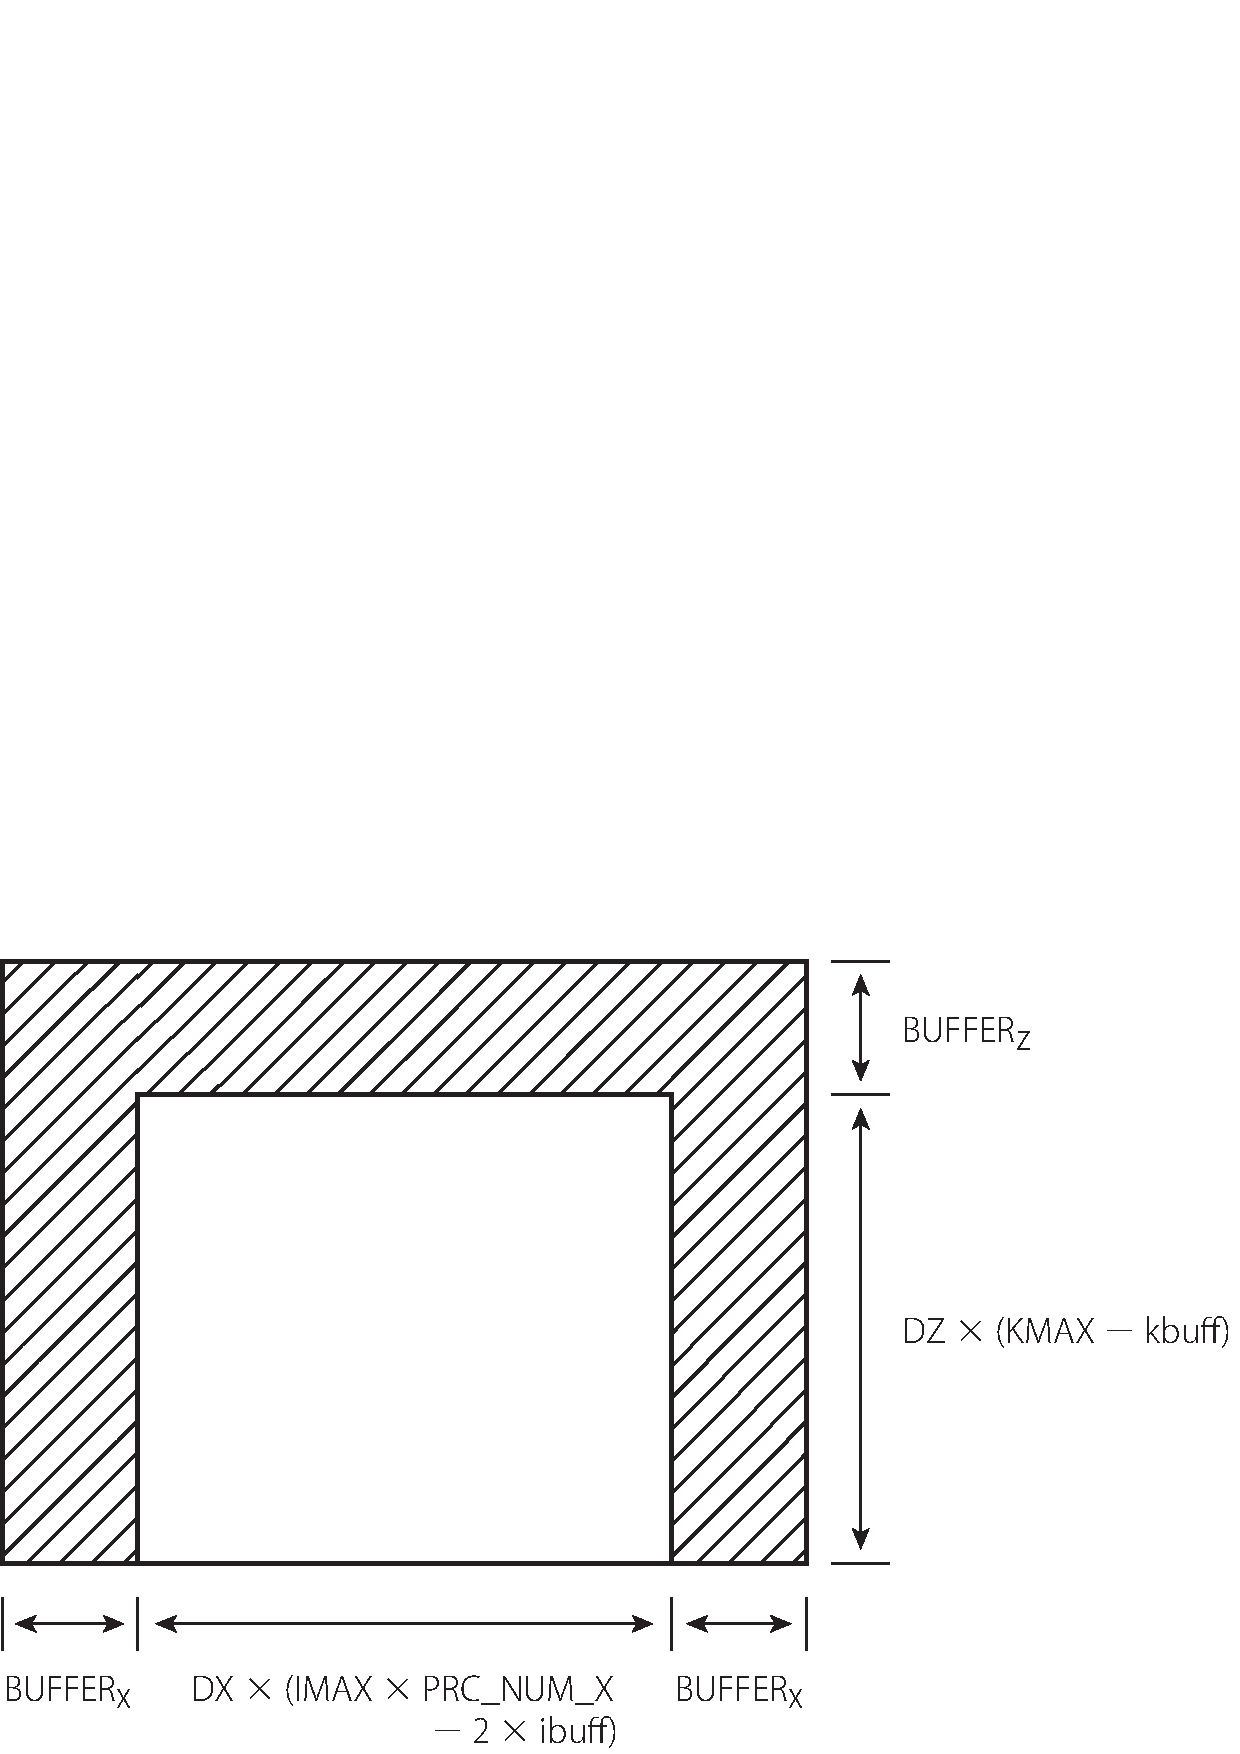
\includegraphics[width=0.8\hsize]{./figure/buffer_xz.pdf}\\
  \caption{Location of the buffer region in the entire calculation domain: the shaded area indicates the buffer region. This figure shows the XZ cross-section. It is the same as the YZ cross-section.}
  \label{fig:buff_xz}
\end{center}
\end{figure}

In general, there is no clear criterion for setting the width and locating grids in the buffer region.
This depends on a problem to be solved.
In \scalerm, the followings are recommended: the number of grids in the vertical buffer region at the top of the model is greater than 5, whereas that in the lateral boundaries is approximately 20$\sim$40.
Depending on the experiment, it may be necessary to increase the number of grids in the buffer region, to increase the buffer region itself by using the appropriate stretch factor, to tune relaxation time, and so on.
The relaxation time is explained below.



The grid intervals in the buffer region are the same as \nmitem{DX, DY, DZ} in \namelist{PARAM_ATMOS_GRID_CARTESC} by default.
But, it is possible for them to be stretched by setting \nmitem{BUFFFACT} $>$ 1. This specification of \nmitem{BUFFFACT} is applied in all directions if the grid intervals are uniformly specified. When the stretched factor is configured separately in every direction, specify \nmitem{BUFFFACT_X, BUFFFACT_Y, BUFFFACT_Z}. Note that in case of the configuration of vertical levels by giving \nmitem{FZ(:)} (refer to \ref{subsec:gridinterv}), the above stretched settings have no effect along the vertical direction.

The grid interval \verb|BDX| in the buffer region is determined as follows:
\begin{eqnarray}
 \verb|BDX(|n\verb|)| &=& \verb|DX| \times \verb|BUFFFACT|^n, \nonumber
\end{eqnarray}
where $n$ denotes the index of grids in the buffer region, in the order directed from the inner to the outer region in the domain. The grid interval is the same as the inner domain at \nmitem{BUFFFACT=1.0}, whereas it increases from the inner to the outer region by a factor of 1.2 at \nmitem{BUFFFACT=1.2}.  Although any value of \nmitem{BUFFFACT} can be configured, the value from 1.0 to 1.2 is recommended to avoid numerical instability.

Finally, the width of the buffer region $\verb|BUFFER|_{\verb|X|}$ is as follows:
\begin{eqnarray}
  \verb|BUFFER|_{\verb|X|} = \nmitemeq{DX} \times \frac{ \nmitemeq{BUFFFACT}^{\texttt{\detokenize{ibuff}}}-1}{ \nmitemeq{BUFFFACT}-1 }
\end{eqnarray}
Even if the same width of buffer region \nmitem{BUFFER_DX} is specified, the number of grids in the buffer region decreases with increasing \nmitem{BUFFFACT}.
When given by \nmitem{BUFFER_NX}, only the width of buffer region is changed.



\subsubsection{Nudging Methods in Buffer Region}

\namelist{PARAM_ATMOS_BOUNDARY} has parameters to configure the nudging in the buffer region.
The boundary data type is configurable by \nmitem{ATMOS_BOUNDARY_TYPE} in \namelist{PARAM_ATMOS_BOUNDARY} (Table \ref{tab:nml_atmos_boundary_type}.)

\begin{table}[h]
\begin{center}
\caption{Choices of the boundary data type}
\label{tab:nml_atmos_boundary_type}
\begin{tabularx}{150mm}{lXX} \hline
  \rowcolor[gray]{0.9} Value & Description of type \\ \hline
  \verb|NONE|    & Do not nudge \\
  \verb|CONST|   & Nudge to a prescribed constant value \\
  \verb|INIT|    & Nudge to the initial value \\
  \verb|OFFLINE| & Nudge to value read from a file (temporally unchanged) \\
  \verb|REAL|    & Nudge to time-dependent value of the parent model or domain \\
  \hline
\end{tabularx}
\end{center}
\end{table}


The following is the parameters in \namelist{PARAM_ATMOS_BOUNDARY}.
\editboxtwo{
  \verb|&PARAM_ATMOS_BOUNDARY | & \\
  \verb| ATMOS_BOUNDARY_TYPE = 'NONE',         | & ; The boundary data type. See Table \ref{tab:nml_atmos_boundary_type}. \\
  \verb| ATMOS_BOUNDARY_IN_BASENAME = '',      | & ; File name of the boundary data for \verb|OFFLINE| or \verb|REAL| type \\
  \verb| ATMOS_BOUNDARY_IN_CHECK_COORDINATES | \textbackslash \\
  ~~\verb|                   = .true.,| & ; Flag to check coordinate variables in the boundary data file. \\
  \verb| ATMOS_BOUNDARY_START_DATE | \textbackslash \\
  ~~\verb|        = (/ -9999, 0, 0, 0, 0, 0 /),| & ; Start time of the boundary data. Only for \verb|REAL| type. \\
  \verb| ATMOS_BOUNDARY_UPDATE_DT = 0.0D0,     | & ; Time interval of the boundary data. Only for \verb|REAL| type. \\
  \verb| ATMOS_BOUNDARY_INTERP_TYPE | \textbackslash \\
  ~~\verb|                  = 'lerp_initpoint',| & ; Temporal interpolation type. \\
                                                 &  ~\verb|same_parent|: use the latest step value (no interpolation), \\
                                                 &  ~\verb|nearest_neighbor|: use the value of the nearest time step, \\
                                                 &  ~\verb|lerp_initpoint|: linear interpolation between values at two time steps as the values are snapshot, \\
                                                 &  ~\verb|lerp_midpoint|: same as \verb|lerp_initpoint| but the values are temporal average during the time step for boundary data. \\
  \verb| ATMOS_BOUNDARY_OUT_BASENAME = '',     | & ; File name to output the initial boundary data. \\
  \verb| ATMOS_BOUNDARY_OUT_TITLE | \textbackslash \\
  ~~\verb|     = 'SCALE-RM BOUNDARY CONDITION',| & ; Title for the output file. \\
  \verb| ATMOS_BOUNDARY_OUT_DTYPE = 'DEFAULT', | & ; Data type (\verb|REAL4| or \verb|REAL8|) for the output. \\
  \verb| ATMOS_BOUNDARY_USE_DENS = .false.,    | & ; Switch of the nudging for the density. \\
  \verb| ATMOS_BOUNDARY_USE_VELZ = .false.,    | & ; Switch for the w. \\
  \verb| ATMOS_BOUNDARY_USE_VELX = .false.,    | & ; Switch for the u. \\
  \verb| ATMOS_BOUNDARY_USE_VELY = .false.,    | & ; Switch for the v. \\
  \verb| ATMOS_BOUNDARY_USE_PT = .false.,      | & ; Switch for the $\theta$. \\
  \verb| ATMOS_BOUNDARY_USE_QV = .false.,      | & ; Switch for the vapor. \\
  \verb| ATMOS_BOUNDARY_USE_QHYD = .false.,    | & ; Switch for the hydrometeors. \\
  \verb| ATMOS_BOUNDARY_VALUE_VELZ = 0.0D0,    | & ; Value of the w. Only for \verb|CONST| type. \\
  \verb| ATMOS_BOUNDARY_VALUE_VELX = 0.0D0,    | & ; Value of the u. Only for \verb|CONST| type. \\
  \verb| ATMOS_BOUNDARY_VALUE_VELY = 0.0D0,    | & ; Value of the v. Only for \verb|CONST| type. \\
  \verb| ATMOS_BOUNDARY_VALUE_PT = 300.0D0,    | & ; Value of the $\theta$. Only for \verb|CONST| type. \\
  \verb| ATMOS_BOUNDARY_VALUE_QTRC =   0.0D0,  | & ; Value of the vapor. Only for \verb|CONST| type. \\
  \verb| ATMOS_BOUNDARY_ALPHAFACT_DENS = 1.0D0,| & ; Factor of the $1/\tau$ for the density. \\
  \verb| ATMOS_BOUNDARY_ALPHAFACT_VELZ = 1.0D0,| & ; Factor for the w. \\
  \verb| ATMOS_BOUNDARY_ALPHAFACT_VELX = 1.0D0,| & ; Factor for the u. \\
  \verb| ATMOS_BOUNDARY_ALPHAFACT_VELZ = 1.0D0,| & ; Factor for the v. \\
  \verb| ATMOS_BOUNDARY_ALPHAFACT_PT = 1.0D0,  | & ; Factor for the $\theta$. \\
  \verb| ATMOS_BOUNDARY_ALPHAFACT_QTRC = 1.0D0,| & ; Factor for the vapor. \\
  \verb| ATMOS_BOUNDARY_SMOOTHER_FACT = 0.2D0, | & ; Factor of the horizontal smoother against the pointwise difference. \\
  \verb| ATMOS_BOUNDARY_FRACZ = 1.0D0,         | & ; Fraction for the nudging region to the buffer region in the z-direction. \\
  \verb| ATMOS_BOUNDARY_FRACX = 1.0D0,         | & ; Fraction in the x-direction. \\
  \verb| ATMOS_BOUNDARY_FRACY = 1.0D0,         | & ; Fraction in the y-direction. \\
  \verb| ATMOS_BOUNDARY_TAUZ = DT * 10.0D0,    | & ; Time scale of the nudging at the top boundary (in second). \\
  \verb| ATMOS_BOUNDARY_TAUX = DT * 10.0D0,    | & ; Time scale at the western and eastern boundary. \\
  \verb| ATMOS_BOUNDARY_TAUY = DT * 10.0D0,    | & ; Time scale at the southern and northern boundary. \\
  \verb| ATMOS_BOUNDARY_LINEAR_V = .false.,    | & ; Profile type of the time scale in the z-direction. If \verb|.true.|, it is a linear profile, otherwise a sinusoidal profile. \\
  \verb| ATMOS_BOUNDARY_LINEAR_H = .false.,    | & ; Profile type in the x- and y-direction. If \verb|.true.|, it is a linear profile, otherwise a exponential profile. \\
  \verb| ATMOS_BOUNDARY_EXP_H = 2.0D0,         | & ; Factor of the exponent of the exponential profile. \\
}

The tendency due to the nudging is written as
\begin{eqnarray}
  \left.\frac{\partial \phi_{k,i,j}}{\partial t}\right|_\mathrm{nudging}
  & = & - \alpha \Delta\phi_{k,i,j} \\ \nonumber
  && + \alpha_s \left( \frac{\Delta\phi_{k,i-1,j} + \Delta\phi_{k,i+1,j} + \Delta\phi_{k,i,j-1} + \Delta\phi_{k,i,j+1}}{8} - \frac{\Delta\phi_{k,i,j}}{2} \right),
\label{eq:nudging}
\end{eqnarray}
where $\Delta\phi$ is difference from the boundary data and $\alpha_s = \alpha \times \nmitemeq{ATMOS_BOUNDARY_SMOOTHER_FACT}$.
The $\alpha$ is the maximum of those in the tree directions $\alpha_x, \alpha_y$ and $\alpha_z$.
The $\alpha$s depend on a length scale $e$ as
\begin{equation}
  e = \max\left( 1 - \frac{d}{\texttt{BUFFER} \times \nmitemeq{ATMOS_BOUNDARY_FRAC}}, 0 \right),
\end{equation}
where $d$ is distance from the boundary.
If \nmitem{ATMOS_BOUNDARY_LINEAR_V} = \verb|.true.|,
\begin{equation}
  \alpha_z = e_z / \tau_z,
\end{equation}
otherwise
\begin{equation}
  \alpha_z =  \sin^2(\pi e_z/2) / \tau_z,
\end{equation}
where $\tau_z$ is \nmitem{ATMOS_BOUNDARY_TAUZ}.
For the horizontal direction, if \nmitem{ATMOS_BOUNDARY_LINEAR_H} = \verb|.true.|,
\begin{equation}
  \alpha_x = e_x / \tau_x,
\end{equation}
otherwise
\begin{equation}
  \alpha_x = e_x \exp\{ - (1-e_x) \times \nmitemeq{ATMOS_BOUNDARY_EXP_H} \} / \tau_x.
\end{equation}
$\alpha_y$ is derived by the same way as $\alpha_x$.

The $\tau$ is the relaxation time at the boundary ($d=0$) with which the difference between the simulated value and the boundary value becomes $1/e$.
On the other hand, two grid scale component of $\Delta \phi$ becomes $1/e$ with the time of $\tau/\nmitemeq{ATMOS_BOUNDARY_SMOOTHER_FACT}$ by the second term of the right-hand side of Eq. \ref{eq:nudging}.
The default value of the $\tau$ is ten times of \nmitem{TIME_DT}.
Please refer to Section \ref{sec:timeintiv} for \nmitem{TIME_DT}.


If \nmitem{ATMOS_BOUNDARY_TYPE} in \namelist{PARAM_ATMOS_BOUNDARY} is \verb|REAL|, the nudging at the top and lateral boundaries for the horizontal velocities, potential temperature, and vapor is applied.
If the simulation is on a daughter domain of the online nesting (See Section \ref{subsec:nest_online}), the same setting is applied with the \verb|REAL| boundary type.


There exists a similar dumping method at near the top boundary, i.e., Rayleigh dumping. See Section \ref{subsec:raydamp}.

\section{Setting the map projection} \label{subsec:adv_mapproj}
%------------------------------------------------------

In \scalerm, grids are allocated based on actual distance. The latitude and longitude for all grids are calculated by using the latitude and longitude of a certain reference point using a map projection. All information pertaining to the latitude and longitude of the grids are output to all output files in \netcdf format. The locations of the domain and the map projection can be configured in \nmitem{PARAM_MAPPROJECTION}. \textcolor{blue}{This configuration must be shared among the configuration files \texttt{pp.conf}, \texttt{init.conf}, and \texttt{run.conf}.} An example is as follows:
\editboxtwo{
\verb|&PARAM_MAPPROJECTION| & \\
\verb| MAPPROJECTION_basepoint_lon = 138.727778D0,| & \\
\verb| MAPPROJECTION_basepoint_lat = 35.360556D0,|  & \\
\verb| MAPPROJECTION_type          = 'MER',|        & ; Choose from Table \ref{tab:map_proj}.\\
\verb|/| & \\
}

\begin{table}[htb]
\begin{center}
\caption{Map projections selectable in \scalerm}
\begin{tabularx}{150mm}{|l|X|} \hline
 \rowcolor[gray]{0.9} \verb|MAPPROJECTION_type| & Map projection\\ \hline
 \verb|NONE| & No map projection for ideal experiment ( default ) \\ \hline
 \verb|LC|   & Lambert conformal conic projection   \\ \hline
 \verb|PS|   & Polar stereo projection           \\ \hline
 \verb|MER|  & Mercator projection               \\ \hline
 \verb|EC|   & Equi-rectangular projection        \\ \hline
\end{tabularx}
\label{tab:map_proj}
\end{center}
\end{table}

\nmitem{MAPPROJECTION_basepoint_lat, MAPPROJECTION_basepoint_lon} are the latitude and longitude at a reference point. This reference point is the center of the calculation domain by the default setting.
In \scalerm, the north and south latitudes are expressed by positive and negative values, respectively. The east and west longitudes are also expressed by positive and negative values, respectively. It is possible to express longitude using an angle greater than $180^{\circ}$.
In above setting, the center of the domain is configured at $35.360556^{\circ}$N and $138.727778^{\circ}$E, where N and E denote the north latitude and east longitude, respectively. The entire calculation domain is placed at the center with a specified size.

\nmitem{MAPPROJECTION_type} provides the kind of map projection and \verb|MER| the Mercator projection.
Table \ref{tab:map_proj} shows the selectable map projections in the current version of \scalerm. In the case of the Mercator projection, the standard latitude, to which a cylinder is tangent, is specified as \nmitem{MAPPROJECTION_M_lat} in units of degrees. In general, the standard latitude is set to the Equator.
In \scalerm, \nmitem{MAPPROJECTION_basepoint_lat} is used as standard latitude, unless \nmitem{MAPPROJECTION_M_lat} is explicitly specified. This is because this method is more precise with less distortion than the usual Mercator projection.

The text below explains the Lambert conformal conic projection, the usage frequency of which is highest. The example is the same as that in the file used in the tutorial for the real atmospheric experiment.
\editbox{
\verb|&PARAM_MAPPROJECTION| \\
\verb| MAPPROJECTION_basepoint_lon = 135.220404,| \\
\verb| MAPPROJECTION_basepoint_lat = 34.653396,| \\
\verb| MAPPROJECTION_type          = 'LC',| \\
\verb| MAPPROJECTION_LC_lat1       =  30.0,| \\
\verb| MAPPROJECTION_LC_lat2       =  40.0,| \\
\verb|/| \\
}
In \scalerm, two standard parallels are used for this projection.
The north and south of them are specified in \nmitem{MAPPROJECTION_LC_lat1, MAPPROJECTION_LC_lat2} 
in units of degrees.
In the region between the latitudes, the ratio of the latitudinal to longitudinal length is adjusted to be close to the Earth’s ellipsoid face.


Furthermore, it is possible for the reference point (\nmitem{MAPPROJECTION_basepoint_lon},\\
\nmitem{MAPPROJECTION_basepoint_lat}) to be displaced from the default setting, i.e., domain center as follows:

\editbox{
\verb|&PARAM_MAPPROJECTION| \\
\verb| MAPPROJECTION_basepoint_lon = 135.220404,| \\
\verb| MAPPROJECTION_basepoint_lat = 34.653396,| \\
\verb| MAPPROJECTION_basepoint_x   = 100.0,| \\
\verb| MAPPROJECTION_basepoint_y   = 100.0,| \\
\verb| MAPPROJECTION_type          = 'LC',| \\
\verb| MAPPROJECTION_LC_lat1       = 30.0,| \\
\verb| MAPPROJECTION_LC_lat2       = 40.0,| \\
\verb|/| \\
}

The location of the reference point is specified as the distance from the south-west corner (bottom-left corner).;
\nmitem{MAPPROJECTION_basepoint_x} and \nmitem{MAPPROJECTION_basepoint_y} are the distances in units of meters between the south-west corner and the reference point in \XDIR and in \YDIR, respectively.
If they are not specified, the center of projection corresponds to that of the domain.
Figure \ref{fig:map_lc} shows both cases.

\begin{figure}[t]
\begin{center}
  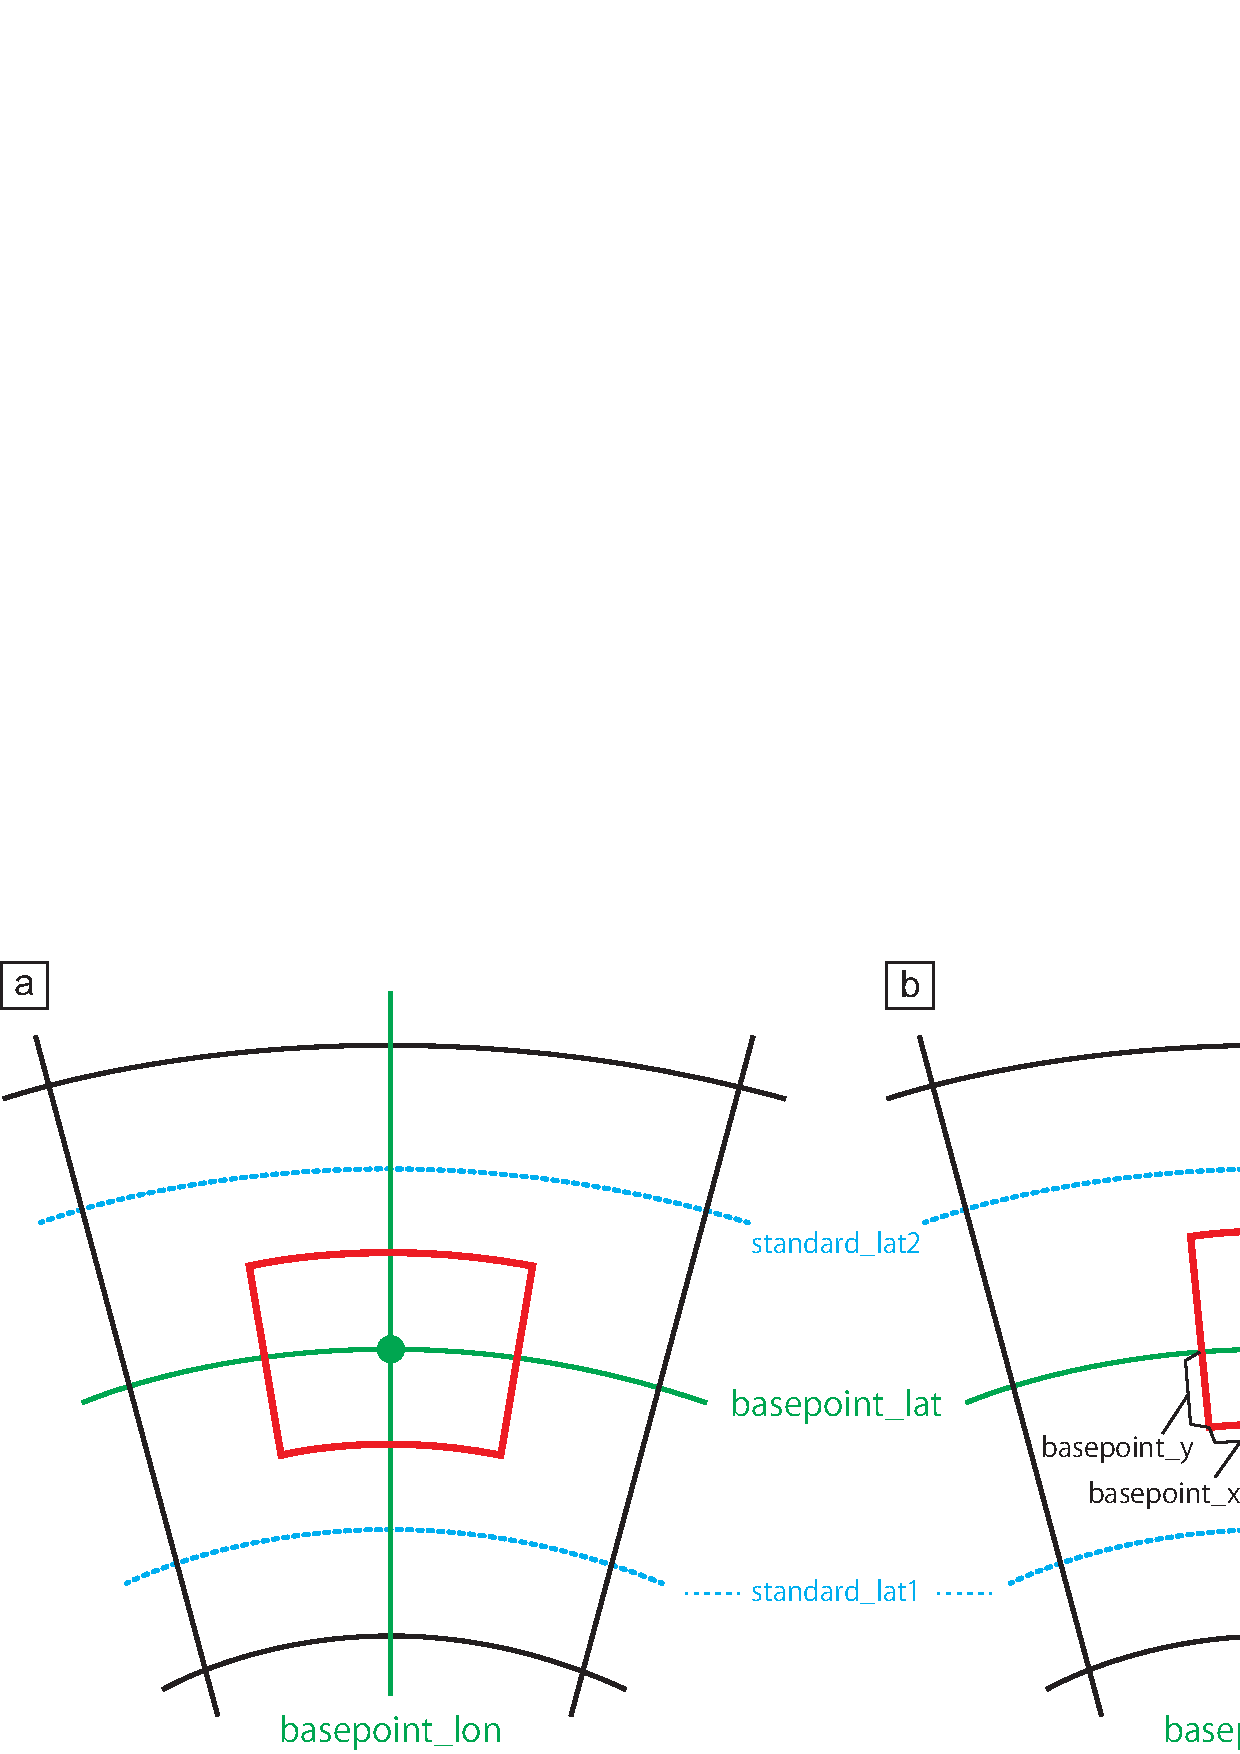
\includegraphics[width=0.8\hsize]{./figure/LC_latlon_xy.pdf}\\
  \caption{The relationship between projection center and calculation domain.; (a) Default setting and (b) the case where the center of projection is displaced at the center of the domain.
    The red line indicates the boundary of the calculation domain.}
  \label{fig:map_lc}
\end{center}
\end{figure}


\section{\SecBasicTopoSetting} \label{subsec:basic_usel_topo}
%-----------------------------------------------------------------------

\scalerm では地形を表現するために、地形に沿った座標系を採用している。
この座標系では、最下層の格子の底面が標高に対して沿うように与えられる。
許容される最大の地形傾斜角度$\theta_{\max}$ [radian]は、次の式で計算する。
\[
  \theta_{\max} = \arctan( \mathrm{RATIO} \times \mathrm{DZ}/\mathrm{DX} )
\]
ここで、$\mathrm{DZ}$と$\mathrm{DX}$はそれぞれ、鉛直方向と水平方向の格子間隔である。
上記の計算式から分かるように、許容される最大傾斜角度は空間解像度に応じて変わる。
$\mathrm{RATIO}$が1.0よりも大きければ地形はより細かく表現され、1.0よりも小さければ粗く表現される。
$\mathrm{RATIO}$を非常に大きく設定した場合には、計算が途中で破綻する危険性が高くなることに注意が必要である。
\scalerm では$\mathrm{RATIO}$のデフォルト値は1.0に設定している。

\verb|scale-rm_pp|は、外部入力する標高データを{\scalelib}形式に変換するためのプログラムである。
詳細な設定は、設定ファイル\verb|pp.conf|の\namelist{PARAM_CNVTOPO}の中で行う。
以下に例を示す。\\

\editboxtwo{
\verb|&PARAM_CNVTOPO                               | & \\
\verb|CNVTOPO_UseGTOPO30            = .true.,      | & ; GTOPO30 データセットを用いるか? \\
\verb|CNVTOPO_UseDEM50M             = .false.,     | & ; DEM50M データセットを用いるか? \\
\verb|CNVTOPO_UseUSERFILE           = .false.,     | & ; ユーザ定義のデータセットを用いるか? \\
\verb|CNVTOPO_smooth_type           = 'LAPLACIAN', | & ; 平滑化のためのフィルタの種類 (OFF,LAPLACIAN,GAUSSIAN) \\
\verb|CNVTOPO_smooth_maxslope_ratio = 10.D0,       | & ; 許容する傾斜の$\mathrm{DZ}$/$\mathrm{DX}$に対する倍率 \\
\verb|CNVTOPO_smooth_maxslope       = -1.D0,       | & ; 許容する傾斜角の最大値 [deg] \\
\verb|CNVTOPO_smooth_local          = .true.,      | & ; 最大傾斜角度を超えた格子でのみ平滑化を続けるかどうか? \\
\verb|CNVTOPO_smooth_itelim         = 10000,       | & ; 平滑化の繰り返し回数の制限値 \\
\verb|CNVTOPO_smooth_hypdiff_niter  = 20,          | & ; 超粘性による平滑化の繰り返し回数 \\
\verb|CNVTOPO_interp_level          = 5,           | & ; 補間に用いる近隣の格子点数 \\
\verb|CNVTOPO_copy_parent           = .false.,     | & ; 子ドメインの緩和領域に親ドメインの地形をコピーするか? \\
\verb|/                                            | \\
}

\scalerm では地形データの入力として、国土地理院が提供する
GTOPO30 と DEM50M に対応している。
プログラム\verb|scale-rm_pp|によってユーザが準備した地形データを変換できる(第\ref{subsec:topo_userfile}節を参照)。
また、上記のデータセットを組み合わせることもできる。
\nmitem{CNVTOPO_UseGTOPO30}と\nmitem{CNVTOPO_UseDEM50M}の両方を
\verb|true|に設定した場合は、プログラムは以下のようにデータを作成する。

\begin{itemize}
 \item GTOPO30 のデータセットを計算領域の格子点に内挿する。
 \item DEM50M が対象とする領域は、DEM50M のデータセットを用いて内挿し、上書きする。
 \item 平滑化を適用する。
\end{itemize}

デフォルトでは、対象とする格子点の周辺にある、入力データの最寄りの5格子点が内挿に使われる。
使用する格子点数は\nmitem{CNVTOPO_interp_level}によって決定される。
地形のリグリッドにおいて、急な傾斜を含む標高を平滑化するためのフィルタとして、
ラプラシアンフィルタとガウスシアンフィルタの2種類が存在する。
これは\nmitem{CNVTOPO_smooth_type}で選択することができ、
デフォルトではラプラシアンフィルタが用いられる。
平滑化の操作において、傾斜角が最大許容角度$\theta_{\max}$を下回るまで、選択されたフィルタが適用される。
\nmitem{CNVTOPO_smooth_maxslope_ratio}を指定することによって、上記の$\mathrm{RATIO}$を直接設定できる。
または、度数で最大傾斜角を決める\nmitem{CNVTOPO_smooth_maxslope}を用いることができる。
平滑化の繰り返し回数の上限はデフォルトでは 10000 回であるが、\nmitem{CNVTOPO_smooth_itelim}を設定することで繰り返し回数を増やせる。
\nmitem{CNVTOPO_smooth_local}を\verb|.true.|に設定した場合は, 繰り返されるフィルタ操作は平滑化が完了していない格子点でのみ続けられる。

小さな空間スケールのノイズを取り除くために、付加的な超粘性を地形に適用する。
シミュレーションにおける数値的なノイズを減らすために、このフィルタリングを行うことを推奨する。
\nmitem{CNVTOPO_smooth_hypdiff_niter}に負の値を設定した場合は、このフィルタは適用されない。

\nmitem{CNVTOPO_copy_parent}は、ネスティング計算のための設定項目である。
一般的に、子ドメインは親ドメインよりも空間解像度が高いために、子ドメインの方が地形がより細かく表現される。
このとき、子ドメインの緩和領域における大気データと親ドメインにおける大気データの間の不整合によって、問題がしばしば起きる。
この問題を回避するために、\nmitem{CNVTOPO_copy_parent}を\verb|.true.|とすれば親ドメインの地形を子ドメインの緩和領域にコピーできる。
親ドメインが存在しない場合は\nmitem{CNVTOPO_copy_parent}を\verb|.false.|に設定しなければならない。
\nmitem{CNVTOPO_copy_parent}を利用する場合の設定は、第\ref{subsec:nest_topo}節で詳しく説明する。


\section{ユーザー定義の地形の準備} \label{subsec:topo_userfile}

\nmitem{CNVTOPO_UseUSERFILE}を\verb|.true.|に設定した場合は、プログラム\verb|scale-rm_pp|は \\
\namelist{PARAM_CNVTOPO_USERFILE}で指定したファイルの変換を行う.

入力データのタイプを\nmitem{USERFILE_TYPE}で指定する。
サポートされているタイプは ``GrADS'' と ``TILE'' である。

``GrADS''タイプを指定した場合、別途入力ファイルのデータ構造を記述するネームリストファイルが必要となる。
このネームリストファイルは\nmitem{USERFILE_GrADS_FILENAME}で指定する。
ネームリストファイルの詳細については、\ref{sec:datainput_grads}を参照のこと。
デフォルトでは、地形、緯度、経度データの変数名のデフォルト値はそれぞれ``topo'', ``lat'', ``lon''であるが、
異なる場合は、それぞれ\nmitem{USERFILE_GrADS_VARNAME}、\nmitem{USERFILE_GrADS_LATNAME}、\nmitem{USERFILE_GrADS_LONNAME}で指定することができる。


``TILE''タイプを指定した場合、カタログファイルが必要である。
カタログファイルには、それぞれのタイルデータファイルの名前およびそれぞれがカバーする領域についての情報が記述されている。
同じ形式である GTOPO30 や DEM50 のカタログファイルを参照するとよい。
以下はカタログファイルの例である。
\editboxtwo{
\verb|001 -90.0  0.0 -180.0   0.0 TILE_sw.grd| & ; 南緯90--0 西経180--0 の範囲, ファイル名 \verb|TILE_sw.grd| \\
\verb|002 -90.0  0.0    0.0 180.0 TILE_se.grd| & ; 南緯90--0 東経0--180 の範囲, ファイル名 \verb|TILE_se.grd| \\
\verb|003   0.0 90.0 -180.0   0.0 TILE_nw.grd| & ; 北緯0--90 西経180--0 の範囲, ファイル名 \verb|TILE_nw.grd| \\
\verb|004   0.0 00.0    0.0 180.0 TILE_ne.grd| & ; 北緯0--90 東経0--180 の範囲, ファイル名 \verb|TILE_ne.grd| \\
}
それぞれのタイルデータは \grads(direct access) 形式と同じ単純なバイナリ形式である。
以下は設定例である。
\editboxtwo{
\verb|&PARAM_CNVTOPO_USERFILE                     | & \\
\verb|USERFILE_CATALOGUE  = "catalogue.txt",      | & ; カタログファイルの名前 \\
\verb|USERFILE_DIR        = "./input_topo",       | & ; 入力ファイルがあるディレクトリのパス \\
\verb|USERFILE_DLAT       = 0.0083333333333333D0, | & ; 格子間隔 (緯度,degree) \\
\verb|USERFILE_DLON       = 0.0083333333333333D0, | & ; 格子間隔 (経度,degree) \\
\verb|USERFILE_DTYPE      = "INT2",               | & ; データの種類 (INT2,INT4,REAL4,REAL8) \\
\verb|USERFILE_yrevers    = .true.,               | & ; データは緯度方向に関して北から南へと格納されているか? \\
\verb|/                                           | \\
}
この例では、\verb|catalogue.txt|という名前のカタログファイルが、ティレクトリ\verb|./input_topo|に存在する。
値は2バイトの整数で格納されている。


%====================================================================================
\section{\SecInputDataSetting} \label{sec:adv_datainput}
%====================================================================================

\begin{table}[htb]
\begin{center}
\caption{\scalelib で対応している外部入力データ}
\begin{tabularx}{150mm}{|l|l|X|} \hline
 \rowcolor[gray]{0.9} データ形式      & \verb|FILETYPE_ORG|  & 備考 \\ \hline
 SCALEデータ形式   & \verb|SCALE-RM|     &  ヒストリファイルのみ対応。latlonカタログを必要とする。 \\ \hline
 バイナリ形式 & \verb|GrADS|        & データ読み込み用のネームリストを別途必要とする。       \\ \hline
% NICAMデータ   & \verb|NICAM-NETCDF| & NetCDF形式の緯度経度格子に変換されたデータに対応する。 \\ \hline
 WRFデータ形式     & \verb|WRF-ARW|      & 「wrfout」、「wrfrst」の両方に対応する。          \\ \hline
\end{tabularx}
\label{tab:inputdata_format}
\end{center}
\end{table}

プログラム\verb|scale-rm_init|は、設定ファイル\verb|init.conf|の設定に従って外部データを初期値・境界値データに変換する。
\verb|scale-rm_init|は、表\ref{tab:inputdata_format}に示される様々な種類の外部データを扱える。
入力データの形式は、\namelist{PARAM_MKINIT_REAL_(ATMOS|OCEAN|LAND)}の\nmitem{FILETYPE_ORG}で指定する。

「SCALEデータ形式」は、主にオフライン・ネスティング実験(第\ref{subsec:nest_offline}節)で使用される。


「バイナリ形式」は、Fortran が直接アクセスできる単精度浮動小数点数のバイナリ形式データである。
具体的な実行例については、チュートリアル(第\ref{sec:tutorial_real_data}節)に記載がある。

「WRFデータ形式」では、WRFによるモデル出力データを直接読み込める。
ただし、そのファイルは、{\scalerm}の境界値データを作成するために必要な全てのデータを含んでいる必要がある。

その他の形式のデータ(例えば、GRIB/GRIB2 データなど)は、バイナリ形式に変換することで {\scalerm} で読み込むことができる。
{\scalelib}の最新版の出力ファイル形式は、バージョン5.3以前の形式とは異なる。
そのため、バージョン5.3以前で作成された初期値/境界値ファイルは本バージョン({\scalelib}{\version})では使用できない。

%%%---------------------------------------------------------------------------------%%%%
\subsubsection{SCALE形式とバイナリ形式で共通の設定} \label{sec:datainput_common_setting}
%%

初期値ファイルに関する設定は、設定ファイル\verb|init.conf|の\namelist{PARAM_RESTART}で行う。
%
\editboxtwo{
\verb|&PARAM_RESTART|                      & \\
\verb| RESTART_OUTPUT       = .false.,|    & ; 初期値(リスタート)ファイルを出力するかどうか\\
\verb| RESTART_OUT_BASENAME = '',|         & ; 初期値(リスタート)ファイルのベース名\\
\verb|/|\\
}
初期値ファイルを作成する場合には、\nmitem{RESTART_OUTPUT}に\verb|.true.|を設定する。
初期値ファイルのベース名は\nmitem{RESTART_OUT_BASENAME}で設定する。
例えば\ref{sec:tutorial_real_intro}節に記述したチュートリアルでは、\nmitem{RESTART_OUT_BASENAME} = ``\verb|init_d01|''を使用している。
これらの設定は、\scalerm の実行時にリスタートファイルを出力する際にも指定する(詳細は第\ref{sec:restart}章を参照)。
生成される初期値ファイルやリスタートファイルは、同じ構造を持つ。


入力データと境界値ファイルに関する設定は、設定ファイル\verb|init.conf|の\\\namelist{PARAM_MKINIT_REAL_(ATMOS|OCEAN|LAND)}で行う。
%%
\editboxtwo{
\verb|&PARAM_MKINIT_REAL_ATMOS|                                      & \\
\verb| NUMBER_OF_FILES            = 1, |                             & ; 入力ファイルの数\\
\verb| NUMBER_OF_TSTEPS           = 1, |                             & ; 各入力ファイル内のデータの時間ステップ数\\
\verb| FILETYPE_ORG               = '',|                             & ; 表\ref{tab:inputdata_format}から選択\\
\verb| BASENAME_ORG               = '',|                             & ; 入力ファイルに関する情報\\
                                                                     & ~~~ (指定方法は\verb|FILETYPE_ORG|に依存)\\
\verb| BASENAME_ADD_NUM           = .false.,|                        & ; \verb|NUMBER_OF_FILES|=1の時ファイル名に番号付けするかどうか\\
\verb| BASENAME_BOUNDARY          = '',|                             & ; 境界値ファイルのベース名\\
\verb| BOUNDARY_UPDATE_DT         = 0.0,|                            & ; 入力データの時間間隔 [s]\\
\verb| USE_FILE_DENSITY           = .false.,|                        & ; 入力ファイル中の密度データを使用するかどうか\\
\verb| USE_NONHYDRO_DENS_BOUNDARY = .false.,|                        & ; 境界値に静力学平衡を満たさない密度を使用するかどうか\\
\verb| USE_SFC_DIAGNOSES          = .false.,|                        & ; 親モデルの地上診断変数を使用するかどうか\\
\verb| USE_DATA_UNDER_SFC         = .true.,|                         & ; 親モデルの地面より下の値を使用するかどうか\\
\verb| SAME_MP_TYPE               = .false.,|                        & ; (For SCALE形式) 雲微物理スキームは親モデルと同じかどうか\\
\verb| INTRP_TYPE                 = 'LINEAR',|                       & ; 水平内挿の種類 ("\verb|LINEAR|", "\verb|DIST-WEIGHT|") \\
\verb| SERIAL_PROC_READ           = .true.,|                         & ; 入力データへのアクセスをマスタプロセスのみに制限するか\\
\verb|/| & \\
\verb|&PARAM_MKINIT_REAL_OCEAN| & \\
\verb| NUMBER_OF_FILES            = 1, |                             & ; 入力ファイルの数\\
\verb| NUMBER_OF_TSTEPS           = 1, |                             & ; 各入力ファイル内のデータの時間ステップ数\\
\verb| FILETYPE_ORG               = '',|                             & ; 表\ref{tab:inputdata_format}から選択\\
\verb| BASENAME_ORG               = '',|                             & ; 入力ファイルに関する情報\\
                                                                     & ~~~ (指定方法は\verb|FILETYPE_ORG|に依存)\\
\verb| INTRP_OCEAN_SFC_TEMP       = 'off',|                          & ; (For GrADS形式) ("\verb|off|", "\verb|mask|", "\verb|fill|") \\
\verb| INTRP_OCEAN_TEMP           = 'off',|                          & ; (For GrADS形式) ("\verb|off|", "\verb|mask|", "\verb|fill|") \\
\verb| SERIAL_PROC_READ           = .true.,|                         & ; 入力データへのアクセスをマスタプロセスのみに制限するか\\
\verb|/| & \\
\verb|&PARAM_MKINIT_REAL_LAND| & \\
\verb| NUMBER_OF_FILES            = 1, |                             & ; 入力ファイルの数\\
\verb| NUMBER_OF_TSTEPS           = 1, |                             & ; 各入力ファイル内のデータの時間ステップ数\\
\verb| FILETYPE_ORG               = '',|                             & ; 表\ref{tab:inputdata_format}から選択\\
\verb| BASENAME_ORG               = '',|                             & ; 入力ファイルに関する情報\\
                                                                     & ~~~ (指定方法は\verb|FILETYPE_ORG|に依存)\\
\verb| USE_FILE_LANDWATER         = .true.,|                         & ; 入力ファイルの土壌水分を使用するかどうか\\
\verb| INTRP_LAND_TEMP            = 'off',|                          & ; (For GrADS形式) ("\verb|off|", "\verb|mask|", "\verb|fill|") \\
\verb| INTRP_LAND_WATER           = 'off',|                          & ; (For GrADS形式) ("\verb|off|", "\verb|mask|", "\verb|fill|") \\
\verb| INTRP_LAND_SFC_TEMP        = 'off',|                          & ; (For GrADS形式) ("\verb|off|", "\verb|mask|", "\verb|fill|") \\
\verb| ELEVATION_CORRECTION       = .true.,|                         & ; 親モデルの地形との高度差を補正するかどうか \\
\verb| SERIAL_PROC_READ           = .true.,|                         & ; 入力データへのアクセスをマスタプロセスのみに制限するか\\
\verb|/| & \\
}

\nmitem{NUMBER_OF_FILES}は入力ファイルの数である。
プログラム\verb|scale-rm_init|は、\verb|00000|から\nmitem{NUMBER_OF_FILES}-1 までの数字を付けたファイルを順に読み込む。
ただし、\nmitem{NUMBER_OF_FILES}=1の時は、自動的に番号づけは行われないので、番号のついたファイルを使用する場合には\\
\nmitem{BASENAME_ADD_NUM}=\verb|.true.|とする。
\nmitem{NUMBER_OF_TSTEPS}は各ファイル中に保存されているデータの時間ステップ数である。

\nmitem{BOUNDARY_UPDATE_DT}は入力データの時間間隔である。
出力される境界値データは入力データの時間間隔と同じである。
\nmitem{BASENAME_BOUNDARY}は、出力される境界値ファイルのベース名である。
\nmitem{BASENAME_BOUNDARY}を指定しなければ、境界値ファイルは出力されない。
モデル積分を実行するためには、大気変数は少なくとも二時刻分の境界値データが必須である。
一方、海洋・陸面変数については、境界値データが必要かどうかは、実行時に使用するスキームに依存する。

空間補間の種類は、\nmitem{INTRP_TYPE}で設定する。
``\verb|LINEAR|''と ``\verb|DIST-WEIGHT|''が選択できる。
``\verb|LINEAR|''の場合は2次元線形補間が用いられ、``\verb|DIST-WEIGHT|''の場合は隣接$N$点の距離重み付け平均が用いられる。
``\verb|LINEAR|''は、2次元実験データや水平方向に1次元配列に格納された非構造格子データなど、水平方向のいずれかの格子点数が1 (\nmitem{IMAXG}=1 もしくは \nmitem{JMAXG}=1) の場合には使用できない。
距離重み付け平均(``\verb|DIST-WEIGHT|'')の場合、隣接点の数は\namelist{PARAM_COMM_CARTESC_NEST}の\nmitem{COMM_CARTES_NEST_INTERP_LEVEL}で設定する。


\scalerm では、初期値・境界値データの読込はマスタープロセスのみが行い、broadcast通信によって各ノードに情報を伝播する。
この時、特に大規模並列計算システムなどでは、読み込んだ入力データが大きいと、メモリ容量が足りなくなることがある。
\nmitem{SERIAL_PROC_READ}に\verb|.false.|を設定することで、各ノードが自身に必要なデータだけを読み込むようになり、
データ読み込み時のメモリ不足を解消することができる。
ただしファイルIOが増大するため、システムによってはファイルアクセスをロックされる等、パフォーマンスの低下がありうることに注意が必要である。


以上の設定は、\nmitem{BASENAME_BOUNDARY} を除き、\verb|ATMOS|と\verb|OCEAN|もしくは\verb|LAND|の間で共有できる。
つまり、\namelist{PARAM_MKINIT_REAL_(OCEAN|LAND)}でネームリストの項目を指定しなければ、
\namelist{PARAM_MKINIT_REAL_ATMOS}で設定した値を使用する。
\\

\noindent\textbf{\underline{\texttt{PARAM\_MKINIT\_REAL\_ATMOS}\textgt{に関する設定}}}

密度の計算法の設定は、\nmitem{USE_FILE_DENSITY}と\nmitem{USE_NONHYDRO_DENS_BOUNDARY}で行う。
デフォルト設定では両方が\verb|.false.|であり、
初期値・境界値の密度は、読み込んだ温度と比湿データから静水圧平衡 ($\frac{dp}{dz}=-\rho g$) を仮定して計算される。
%(ここで見積った密度は、親モデルの密度とは必ずしも一致しない)。
\nmitem{USE_FILE_DENSITY} = \verb|.true.|の場合、他の変数同様に、
入力ファイルから読み込んだ密度の値を初期値・境界値として使用する。
\nmitem{USE_FILE_DENSITY}の設定にかかわらず、\nmitem{USE_NONHYDRO_DENS_BOUNDARY} = \verb|.true.|とした場合には、
気温、気圧、比湿などの入力データと状態方程式 ($\rho = p/RT$)を用いて、境界値データの密度が計算される(初期値データには影響しない)。
ここで計算された密度は、一般的には親モデルの値と整合的である。
%\nmitem{USE_FILE_DENSITY}=\verb|.false.|かつ\\ \nmitem{USE_FILE_DENSITY}=\verb|.true.|の場合は、初期値データおよび境界値データの密度は異なるものとなる。
このオプションが用意された理由は次の通りである。
多くの場合、計算初期ショックを抑えるため、初期値データは静水圧平衡にある密度を使うことが望ましい。
一方、静水圧平衡により作成した密度は
親モデルの密度(多くの場合、実際の値に近いと期待される)と一致しない場合があり、
これが、\scalerm での計算結果に大きな質量バイアスを生じる可能性がある。
そのような場合、気圧の再現性などの観点において、
\nmitem{USE_NONHYDRO_DENS_BOUNDARY}=\verb|.true.|として親モデルとの整合的な密度を与える方が良い場合がある。
境界値に静水圧平衡からずれた密度を使うことで生じる鉛直加速や波は、境界領域ナッジングにより速やかに減衰されると期待される。


\nmitem{USE_SFC_DIAGNOSES}は親モデルの最下層高度よりも低い層における値の計算のためのスイッチである。
\nmitem{USE_SFC_DIAGNOSES} = \verb|.true.|の場合、T2, RH2, U10, V10, PSFC といった地表面変数が使われる。
そうでない場合には、等温位および静水圧平衡の仮定のもとで計算される。
\nmitem{USE_DATA_UNDER_SFC}は、入力データ中の地表よりも低い層のデータを使うか無視するかを決めるのスイッチである。
%地表よりも低いデータは、高い山岳域において、高い気圧面で現れることがある。
\\

\noindent\textbf{\underline{\texttt{PARAM\_MKINIT\_REAL\_LAND}\textgt{に関する設定}}}

土壌水分の設定は、\namelist{PARAM_MKINIT_REAL_LAND}の\nmitem{USE_FILE_LANDWATER}で行う。
土壌水分データの与え方は、(1)親モデルの値など入力データとして与える方法(\nmitem{USE_FILE_LANDWATER} = \verb|.true.|)と、
(2)領域全体で一定値を与える方法(\nmitem{USE_FILE_LANDWATER} = \verb|.false.|)の2種類ある。
(1)の場合には、3次元の土壌水分データとして、
体積含水率(\verb|SMOISVC|)か飽和度(\verb|SMOISDS|)のどちらかを用意する必要がある。
ここで、体積含水率は土の体積$V$の中に占める水の体積$V_w$の割合($V_w / V$)、
飽和度は$V$の中に占める間隙の体積$V_v$に対する水の体積$V_w$の割合($V_w / V_v$)である。
%
(2)の場合には、以下の例のように、飽和度を\verb|INIT_LANDWATER_RATIO| で指定する。
デフォルト値は 0.5 である。
土壌の空隙率($V_v/V$)は、土地利用に応じて変わる。
\editboxtwo{
\verb|&PARAM_MKINIT_REAL_LAND| & \\
\verb| USE_FILE_LANDWATER   = .true. | & ; 土壌水分をファイルから読むかどうか \\
\verb| INIT_LANDWATER_RATIO = 0.5    | & ; \verb|USE_FILE_LANDWATER=.false.|の場合の飽和度\\
\verb|  .....略.....                 | &  \\
\verb|/| & \\
}

初期値・境界値データの土壌温度・地表面気温の作成において、
親モデルの地形との高度差に応じた補正を行うかは、\namelist{PARAM_MKINIT_REAL_LAND}の\nmitem{ELEVATION_CORRECTION}で指定する。
親モデルの地形と\scalerm が作成する地形は一般には異なるため、親モデルの土壌温度・地表面気温をそのまま内挿して初期値・境界値データを作成した場合、
高度差の分だけ不整合が生じる。
\nmitem{ELEVATION_CORRECTION}を\verb|.true.|にした場合、初期値・境界値データの土壌温度・地表面気温は高度差に応じて補正される。
例えば、\scalerm が作成した地形が親モデルの地形よりも$\Delta h$高い場合、
土壌温度・地表面気温は$\Delta h\Gamma$($\Gamma$は国際標準大気の温度減率:$\Gamma=6.5\times 10^{-3}$ [K/m])の分だけ一様に減じられる。
デフォルト設定は\nmitem{ELEVATION_CORRECTION} = \verb|.true.|である。


%%%---------------------------------------------------------------------------------%%%%
\subsubsection{SCALE形式データの入力} \label{sec:datainput_scale}

SCALE 形式データの\namelist{PARAM_MKINIT_REAL_(ATMOS|OCEAN|LAND)}の設定例は以下の通りである。
\editbox{
\verb|&PARAM_MKINIT_REAL_ATMOS|\\
\verb| NUMBER_OF_FILES            = 2, |             \\
\verb| FILETYPE_ORG               = "SCALE-RM",|     \\
\verb| BASENAME_ORG               = "history_d01",|  \\
\verb| BASENAME_ADD_NUM           = .true.,|         \\
\verb| BASENAME_BOUNDARY          = 'boundary_d01',| \\
\verb| SAME_MP_TYPE               = .false.,|        \\
... \\
\verb|/|\\
\verb|&PARAM_MKINIT_REAL_OCEAN|\\
\verb| FILETYPE_ORG               = "SCALE-RM",|     \\
\verb| BASENAME_ORG               = "history_d01",|  \\
... \\
\verb|/|\\
\verb|&PARAM_MKINIT_REAL_LAND|\\
\verb| FILETYPE_ORG               = "SCALE-RM",|     \\
\verb| BASENAME_ORG               = "history_d01",|  \\
... \\
\verb|/|\\
}

\nmitem{FILETYPE_ORG}は、\verb|"SCALE-RM"|に設定する。
入力ファイルのベース名は、\nmitem{BASENAME_ORG}で指定する。
\verb|BASENAME_ORG|を\verb|"history_d01"|としたならば、
入力ファイル数が1の場合、そのファイルは「\verb|history_d01.nc|」というファイル名で準備する。
入力ファイルが複数ある場合や\nmitem{BASENAME_ADD_NUM} = \verb|.true.|とした場合には、
「\verb|history_d01_XXXXX.nc|」と\verb|00000|から番号付けされた入力ファイルを準備する。

使用する雲微物理スキームが親モデルと同じである場合は、\nmitem{SAME_MP_TYPE}に\verb|.true.|を指定する。


%%%---------------------------------------------------------------------------------%%%%
\subsubsection{バイナリ形式データの入力} \label{sec:datainput_grads}

バイナリデータを入力ファイルとして用いる場合は、
GrADSで使われる形式に従ってデータを用意しておく必要がある。
GrADSのデータ形式は、\url{http://cola.gmu.edu/grads/gadoc/aboutgriddeddata.html#structure}を参照いただきたい。

GrADS 形式データの\namelist{PARAM_MKINIT_REAL_(ATMOS|OCEAN|LAND)}の設定例は以下の通りである。
\editbox{
\verb|&PARAM_MKINIT_REAL_ATMOS|\\
\verb| NUMBER_OF_FILES            = 2, |     \\
\verb| FILETYPE_ORG               = "GrADS",|\\
\verb| BASENAME_ORG               = "namelist.grads_boundary.FNL.2005053112-2015011400",|\\
\verb| BASENAME_ADD_NUM           = .true.,| \\
\verb| BASENAME_BOUNDARY          = 'boundary_d01',| \\
\verb| BOUNDARY_UPDATE_DT         = 21600.0,|\\
... \\
\verb|/|\\
\verb|&PARAM_MKINIT_REAL_OCEAN|\\
\verb| FILETYPE_ORG               = "GrADS",|\\
\verb| BASENAME_ORG               = "namelist.grads_boundary.FNL.2005053112-2015011400",|\\
\verb| INTRP_OCEAN_SFC_TEMP       = "mask",|\\
\verb| INTRP_OCEAN_TEMP           = "mask",|\\
... \\
\verb|/|\\
\verb|&PARAM_MKINIT_REAL_LAND|\\
\verb| FILETYPE_ORG               = "GrADS",|\\
\verb| BASENAME_ORG               = "namelist.grads_boundary.FNL.2005053112-2015011400",|\\
\verb| INTRP_LAND_TEMP            = "fill",|\\
\verb| INTRP_LAND_WATER           = "fill",|\\
\verb| INTRP_LAND_SFC_TEMP        = "fill",|\\
... \\
\verb|/|\\
}

\nmitem{FILETYPE_ORG}は\verb|"GrADS"|に設定する。
\scalerm では、バイナリデータ({\grads}形式)のファイル名やデータ構造について、
「ctl」ファイルの代わりに、\nmitem{BASENAME_ORG}で指定するネームリストファイルで指定する。
ネームリストファイルは、予め用意しておく必要がある。


バイナリデータのファイル名やデータ構造の情報を与える
ネームリストファイル(\verb|namelist.grads_boundary*|)の一例を下記に示す。
\editbox{
\verb|#| \\
\verb|# Dimension    |  \\
\verb|#|                \\
\verb|&GrADS_DIMS|  \\
\verb| nx     = 360,|~~~   ; Default value of the number of grids in the x direction \\
\verb| ny     = 181,|~~~   ; Default value of the number of grids in the y direction \\
\verb| nz     = 26, |~~~~~ ; Default value of the number of layers in the z direction \\
\verb|/|                \\
\\
\verb|#              |  \\
\verb|# Variables    |  \\
\verb|#              |  \\
\verb|&GrADS_ITEM  name='lon',     dtype='linear',  swpoint=0.0d0,   dd=1.0d0 /  |  \\
\verb|&GrADS_ITEM  name='lat',     dtype='linear',  swpoint=90.0d0,  dd=-1.0d0 / |  \\
\verb|&GrADS_ITEM  name='plev',    dtype='levels',  lnum=26,| \\
~~~\verb|      lvars=100000,97500,.........,2000,1000, /     |  \\
\verb|&GrADS_ITEM  name='HGT',     dtype='map',     fname='FNLatm', startrec=1,  totalrec=125 / |  \\
\verb|&GrADS_ITEM  name='U',       dtype='map',     fname='FNLatm', startrec=27, totalrec=125 / |  \\
\verb|&GrADS_ITEM  name='V',       dtype='map',     fname='FNLatm', startrec=53, totalrec=125 / |  \\
\verb|&GrADS_ITEM  name='T',       dtype='map',     fname='FNLatm', startrec=79, totalrec=125 / |  \\
\verb|&GrADS_ITEM  name='RH',      dtype='map',     fname='FNLatm', startrec=105,totalrec=125, nz=21 /  |  \\
\verb|&GrADS_ITEM  name='MSLP',    dtype='map',     fname='FNLsfc', startrec=1,  totalrec=9   / |  \\
\verb|&GrADS_ITEM  name='PSFC',    dtype='map',     fname='FNLsfc', startrec=2,  totalrec=9   / |  \\
\verb|&GrADS_ITEM  name='SKINT',   dtype='map',     fname='FNLsfc', startrec=3,  totalrec=9   / |  \\
\verb|&GrADS_ITEM  name='topo',    dtype='map',     fname='FNLsfc', startrec=4,  totalrec=9   / |  \\
\verb|&GrADS_ITEM  name='lsmask',  dtype='map',     fname='FNLsfc', startrec=5,  totalrec=9  /  |  \\
\verb|&GrADS_ITEM  name='U10',     dtype='map',     fname='FNLsfc', startrec=6,  totalrec=9   / |  \\
\verb|&GrADS_ITEM  name='V10',     dtype='map',     fname='FNLsfc', startrec=7,  totalrec=9   / |  \\
\verb|&GrADS_ITEM  name='T2',      dtype='map',     fname='FNLsfc', startrec=8,  totalrec=9   / |  \\
\verb|&GrADS_ITEM  name='RH2',     dtype='map',     fname='FNLsfc', startrec=9,  totalrec=9   / |  \\
\verb|&GrADS_ITEM  name='llev',    dtype='levels',  lnum=4, lvars=0.05,0.25,0.70,1.50, /        |  \\
~~~~~~~~\verb| missval=9.999e+20 /|  \\
\verb|&GrADS_ITEM  name='STEMP',   dtype='map',     fname='FNLland', nz=4, startrec=1, totalrec=8,|\\
~~~~~~~~\verb| missval=9.999e+20 /|  \\
\verb|&GrADS_ITEM  name='SMOISVC', dtype='map',     fname='FNLland', nz=4, startrec=5, totalrec=8,|\\
~~~~~~~~\verb| missval=9.999e+20 /|  \\
}


格子数のデフォルト値は\namelist{GrADS_DIMS}の\verb|nx, ny, nz|で指定する。
また、入力データに関する設定は、各変数ごとに\namelist{GrADS_ITEM}を用意し指定する。
\namelist{GrADS_ITEM}に関する説明は、表\ref{tab:namelist_grdvar}に示す。

入力ファイルのベース名は、ネームリストファイル内の\verb|fname|で設定する。
\verb|fname="filename"| と指定されている場合、
入力ファイルが1つのとき(\nmitem{NUMBER_OF_FILES}=1)は、入力ファイルは「\verb|filename.grd|」という名前で準備する。
入力ファイルが複数あるとき、もしくは、\nmitem{BASENAME_ADD_NUM} = \verb|.true.|の場合には、
「\verb|filename_XXXXX.grd|」と番号付けされたファイルを準備する。

ある変数の格子数がデフォルト値と異なる場合には、\namelist{GrADS_ITEM}の\verb|nx, ny, nz|でその変数の格子数を設定する。
例えば、ある層から上では、比湿(QV)や相対湿度(RH)のデータが利用できない場合がある。
その場合には、データが存在する層数を\verb|nz|で指定する。

\verb|nz|より上層でのQVの与え方は、\namelist{PARAM_MKINIT_REAL_GrADS}の\nmitem{upper_qv_type}で指定される。
\nmitem{upper_qv_type}=\verb|ZERO|の場合、QV=0と設定される。
\nmitem{upper_qv_type}=\verb|COPY|の場合、湿度の入力データが存在する最上層のRHをデータの存在しない上層にコピーして、
QV の値を決める。
デフォルトの設定は'\verb|ZERO|'である。
\editboxtwo{
\verb|&PARAM_MKINIT_REAL_GrADS|  & \\
\verb| upper_qv_type = "ZERO"|   & ; \verb|nz|より上層でのQVの与え方\\
                                 & ~~~("\verb|ZERO|", "\verb|COPY|")\\
\verb|/|\\
}


\scalerm の計算に必要な変数のリストは、表\ref{tab:grdvar_item}に示す。
%
{\small
\begin{table}[!h]
\begin{center}
\caption{\namelist{GrADS_ITEM}の変数}
\label{tab:namelist_grdvar}
\begin{tabularx}{150mm}{lXl} \hline
\rowcolor[gray]{0.9} \verb|GrADS_ITEM|の項目  & 説明   & 備考                                     \\ \hline
name     & 変数名                                      & 表\ref{tab:grdvar_item}より選択          \\
dtype    & データタイプ                                & \verb|"linear"|, \verb|"levels"|, \verb|"map"|から選択 \\\hline\\\hline
\multicolumn{3}{l}{\nmitem{dtype}が\verb|"linear"|の場合のネームリスト (\verb|"lon", "lat"|専用)} \\ \hline
fname    & ファイル名の頭                              &                 \\
swpoint  & スタートポイントの値                        &                 \\
dd       & 増分                                        &                 \\ \hline\\\hline
\multicolumn{3}{l}{\nmitem{dtype}が\verb|"levels"|の場合のネームリスト (\verb|"plev", "llev"|専用)} \\ \hline
lnum     & レベルの数(層数)                            &                 \\
lvars    & 各層の値                                    &                 \\ \hline\\\hline
\multicolumn{3}{l}{\nmitem{dtype}が\verb|"map"|の場合のネームリスト}     \\ \hline
startrec & 変数\nmitem{item}のレコード番号             & t=1 の時刻の値  \\
totalrec & 一時刻あたりの全変数のレコード長            &                 \\
missval  & 欠陥値の値                                 & (オプション)    \\ \hline
nx       & x方向の格子数                               & (オプション)    \\ \hline
ny       & y方向の格子数                               & (オプション)    \\ \hline
nz       & z方向の層数                                 & (オプション)    \\ \hline
yrev     & データが北から南の順に記録されている場合は\verb|.true.|とする & (オプション)\\ \hline
\end{tabularx}
\end{center}
\end{table}
}


{\small
\begin{table}[!h]
\begin{center}
\caption{\namelist{GrADS_ITEM}の\nmitem{name}の変数リスト。
アスタリスクは「オプションであるが、可能な限り推奨される」ことを意味する。
二重のアスタリスクは、「利用できるが、推奨されない」ことを意味する。
}
\label{tab:grdvar_item}
\begin{tabularx}{150mm}{rl|l|l|X} \hline
 \rowcolor[gray]{0.9} & 変数名 \nmitem{name} & 説明 & 単位 & データタイプ \nmitem{dtype} \\ \hline
           &\verb|lon|     & 経度                              & [deg.]   & \verb|linear, map| \\
           &\verb|lat|     & 緯度                              & [deg.]   & \verb|linear, map| \\
           &\verb|plev|    & 気圧                              & [Pa]     & \verb|levels, map| \\
    $\ast$ &\verb|HGT|     & 高度(ジオポテンシャル)            & [m]      & \verb|map| \\
    $\ast$ &\verb|DENS|    & 密度                              & [kg/m3]  & \verb|map| \\
           &\verb|U|       & 東西風速                          & [m/s]    & \verb|map| \\
           &\verb|V|       & 南北風速                          & [m/s]    & \verb|map| \\
$\ast\ast$ &\verb|W|       & 鉛直風速                          & [m/s]    & \verb|map| \\
           &\verb|T|       & 気温                              & [K]      & \verb|map| \\
           &\verb|RH|      & 相対湿度 (QVがある場合は省略可)   & [\%]     & \verb|map| \\
           &\verb|QV|      & 比湿 (RH がある場合は省略可)      & [kg/kg]  & \verb|map| \\
$\ast\ast$ &\verb|QC|      & 雲水の質量比                      & [kg/kg]  & \verb|map| \\
$\ast\ast$ &\verb|QR|      & 雨水の質量比                      & [kg/kg]  & \verb|map| \\
$\ast\ast$ &\verb|QI|      & 雲氷の質量比                      & [kg/kg]  & \verb|map| \\
$\ast\ast$ &\verb|QS|      & 雪の質量比                        & [kg/kg]  & \verb|map| \\
$\ast\ast$ &\verb|QG|      & 霰の質量比                        & [kg/kg]  & \verb|map| \\
$\ast\ast$ &\verb|MSLP|    & 海面更正気圧                      & [Pa]     & \verb|map| \\
$\ast\ast$ &\verb|PSFC|    & 地上気圧                          & [Pa]     & \verb|map| \\
$\ast\ast$ &\verb|U10|     & 10m 東西風速                      & [m/s]    & \verb|map| \\
$\ast\ast$ &\verb|V10|     & 10m 南北風速                      & [m/s]    & \verb|map| \\
$\ast\ast$ &\verb|T2|      & 2m 気温                           & [K]      & \verb|map| \\
$\ast\ast$ &\verb|RH2|     & 2m 相対湿度 (Q2がある場合は省略可) & [\%]    & \verb|map| \\
$\ast\ast$ &\verb|Q2|      & 2m 比湿 (RH2がある場合は省略可)    & [kg/kg] & \verb|map| \\
    $\ast$ &\verb|TOPO|    & GCMの地形                         & [m]      & \verb|map| \\
    $\ast$ &\verb|lsmask|  & GCMの海陸分布                     & 0:海1:陸 & \verb|map| \\
           &\verb|SKINT|   & 地表面温度                        & [K]      & \verb|map| \\
           &\verb|llev|    & 土壌の深さ                        & [m]      & \verb|levels| \\
           &\verb|STEMP|   & 土壌温度                          & [K]      & \verb|map| \\
           &\verb|SMOISVC| & 土壌水分(体積含水率)              & [-]      & \verb|map| \\
           &               & (SMOISDS がある場合は省略可)      &          &            \\
           &\verb|SMOISDS| & 土壌水分(飽和度)                  & [-]      & \verb|map| \\
           &               & (SMOISVC がある場合は省略可)      &          &            \\
           &\verb|SST|     & 海面温度(SKINTがある場合は省略可) & [K]      & \verb|map| \\ \hline
\end{tabularx}
\end{center}
\end{table}
}

\clearpage
%\newpage
\section{\SecBasicIntegrationSetting} \label{sec:timeintiv}
%------------------------------------------------------
積分時間や時間刻み幅は、実験の目的や設定に応じて適切に設定する必要がある。
時間刻み幅は、モデルの空間解像度に依存する。
数値不安定を回避するために、より短い時間刻み幅がしばしば要求される。
積分時間と時間刻み幅は、
シミュレーション実行用の設定ファイルの\namelist{PARAM_TIME}で設定できる。

\editboxtwo{
\verb|&PARAM_TIME| & \\
\verb| TIME_STARTDATE             = 2014, 8, 10, 0, 0, 0,| & 積分を開始する日付:放射過程計算で必要\\
\verb| TIME_STARTMS               = 0.D0,  | & 開始時刻[mili sec]\\
\verb| TIME_DURATION              = 12.0D0,| & 積分時間[単位は\verb|TIME_DURATION_UNIT|で設定]\\
\verb| TIME_DURATION_UNIT         = "HOUR",| & \verb|TIME_DURATION|の単位\\
\verb| TIME_DT                    = 60.0D0,| & 時間積分の時間刻み幅\\
\verb| TIME_DT_UNIT               = "SEC", | & \verb|TIME_DT|の単位 \\
\verb| TIME_DT_ATMOS_DYN          = 30.0D0,| & 力学過程計算の時間刻み幅\\
\verb| TIME_DT_ATMOS_DYN_UNIT     = "SEC", | & \verb|TIME_DT_ATMOS_DYN|の単位\\
\verb| TIME_DT_ATMOS_PHY_CP       = 600.0D0,| & 積雲パラメタリゼーション計算の時間刻み幅 \\
\verb| TIME_DT_ATMOS_PHY_CP_UNIT  = "SEC", | & \verb|TIME_DT_ATMOS_PHY_CP|の単位\\
\verb| TIME_DT_ATMOS_PHY_MP       = 60.0D0,| & 雲物理過程計算の時間刻み幅 \\
\verb| TIME_DT_ATMOS_PHY_MP_UNIT  = "SEC", | & \verb|TIME_DT_ATMOS_PHY_MP|の単位\\
\verb| TIME_DT_ATMOS_PHY_RD       = 600.0D0, | & 放射過程計算の時間刻み幅 \\
\verb| TIME_DT_ATMOS_PHY_RD_UNIT  = "SEC",  | & \verb|TIME_DT_ATMOS_PHY_RD|の単位\\
\verb| TIME_DT_ATMOS_PHY_SF       = 60.0D0, | & 大気下端境界(フラックス)過程計算の時間刻み幅\\
\verb| TIME_DT_ATMOS_PHY_SF_UNIT  = "SEC",  | & \verb|TIME_DT_ATMOS_PHY_SF|の単位\\
\verb| TIME_DT_ATMOS_PHY_TB       = 60.0D0,| & 乱流過程計算の時間刻み幅 \\
\verb| TIME_DT_ATMOS_PHY_TB_UNIT  = "SEC", | & \verb|TIME_DT_ATMOS_PHY_TB|の単位\\
\verb| TIME_DT_ATMOS_PHY_BL       = 60.0D0,| & 混合層過程計算の時間刻み幅 \\
\verb| TIME_DT_ATMOS_PHY_BL_UNIT  = "SEC", | & \verb|TIME_DT_ATMOS_PHY_BL|の単位\\
\verb| TIME_DT_OCEAN              = 300.0D0,| & 海面過程計算の時間刻み幅\\
\verb| TIME_DT_OCEAN_UNIT         = "SEC",  | & \verb|TIME_DT_OCEAN|の単位\\
\verb| TIME_DT_LAND               = 300.0D0,| & 陸面過程計算の時間刻み幅\\
\verb| TIME_DT_LAND_UNIT          = "SEC",  | & \verb|TIME_DT_LAND|の単位\\
\verb| TIME_DT_URBAN              = 300.0D0,| & 都市過程計算の時間刻み幅\\
\verb| TIME_DT_URBAN_UNIT         = "SEC",  | & \verb|TIME_DT_URBAN|の単位\\
\verb| TIME_DT_ATMOS_RESTART      = 21600.D0, | & リスタートファイル(大気)の出力間隔\\
\verb| TIME_DT_ATMOS_RESTART_UNIT = "SEC",    | & \verb|TIME_DT_ATMOS_RESTART|の単位\\
\verb| TIME_DT_OCEAN_RESTART      = 21600.D0, | & リスタートファイル(海面)の出力間隔\\
\verb| TIME_DT_OCEAN_RESTART_UNIT = "SEC",    | & \verb|TIME_DT_OCEAN_RESTART|の単位\\
\verb| TIME_DT_LAND_RESTART       = 21600.D0, | & リスタートファイル(陸面)の出力間隔\\
\verb| TIME_DT_LAND_RESTART_UNIT  = "SEC",    | & \verb|TIME_DT_LAND_RESTART|の単位\\
\verb| TIME_DT_URBAN_RESTART      = 21600.D0, | & リスタートファイル(都市)の出力間隔\\
\verb| TIME_DT_URBAN_RESTART_UNIT = "SEC",    | & \verb|TIME_DT_URBAN_RESTART|の単位\\
\verb| TIME_DT_WALLCLOCK_CHECK      = 21600.D0,            | & 実経過時間を確認する時間間隔\\
\verb| TIME_DT_WALLCLOCK_CHECK_UNIT = "SEC",               | & \verb|TIME_DT_WALLCLOCK_CHECK|の単位\\
\verb| TIME_WALLCLOCK_LIMIT         = 86400.D0,            | & 経過時間の制限 [sec]\\
\verb| TIME_WALLCLOCK_SAFE          = 0.95D0,              | & 経過時間制限に対する安全率 \\
\verb|/|\\
}


\subsection{力学過程に対する時間刻み幅}

\nmitem{TIME_DT} は時間積分に対する時間刻み幅であり、$\Delta t$ と大抵書かれる。
$\Delta t$はトレーサー移流に対する時間刻み幅であり、また全ての物理過程の基本単位でもある。
計算不安定を回避するために、\nmitem{TIME_DT} は、
格子間隔を移流速度の最大値で割った値よりも小さくなければならない。
力学変数の時間積分は移流速度ではなく音速で制約されるため、
力学過程の時間刻み幅\nmitem{TIME_DT_ATMOS_DYN}は$\Delta t$よりも小さく与えるべきである。
\nmitem{TIME_DT_ATMOS_DYN}の値は、計算安定性に関連して時間積分スキームに依存する。
\nmitem{TIME_DT_ATMOS_DYN}の標準的な値として、
\nmitem{ATMOS_DYN_TINTEG_SHORT_TYPE}が\verb|RK4|の場合は最小格子間隔を 420 m/s で割った値、
\verb|RK3| の場合には最小格子間隔を 840 m/s で割った値が目安である。
ただし、\nmitem{TIME_DT_ATMOS_DYN}は、\nmitem{TIME_DT}の約数でなければならないことに注意されたい。
また、\nmitem{TIME_DT}の\nmitem{TIME_DT_ATMOS_DYN}に対する比が大きすぎる場合は
計算不安定がしばしば起きる。
\nmitem{TIME_DT}/\nmitem{TIME_DT_ATMOS_DYN}が、2または3となるように設定することを推奨する。
これらの条件については、第\ref{subsec:cfl_check}節も参照されたい。
\nmitem{TIME_DT_ATMOS_DYN}と\nmitem{TIME_DT_ATMOS_DYN_UNIT}を設定する代わりに、
この比(\nmitem{TIME_DT}/\nmitem{TIME_DT_ATMOS_DYN})を\nmitem{TIME_NSTEP_ATMOS_DYN}で指定することができる。
\nmitem{TIME_NSTEP_ATMOS_DYN}は整数でなければならない。

\subsection{CFL条件の確認} \label{subsec:cfl_check}

移流対する時間刻み幅\nmitem{TIME_DT}は、格子幅を速度で割った値よりも小さくなければならない(すなわち、Courant-Friedrichs-Lewy (CFL) 条件)。
無次元数$U \Delta t/\Delta x$はクーラン数と呼ばれる。
ここで、 $U$は速度, $\Delta x$は格子幅、 $\Delta t$は時間刻み幅である。
CFL条件とは、クーラン数が1よりも小さくなければならないことである。

\scalerm には、クーラン数が制限値を超えているかを確認する機能がある。
この機能を有効にするには、\namelist{PARAM_ATMOS_VARS}の\nmitem{ATMOS_VARS_CHECKCFL_SOFT}や\nmitem{ATMOS_VARS_CHECKCFL_HARD}を設定する。
これらのデフォルト値はそれぞれ、1.0 と 2.0 である。
シミュレーション中にクーラン数が\nmitem{ATMOS_VARS_CHECKCFL_SOFT}を超えれば、
以下のメッセージをログファイルに出力される。
\msgbox{
\verb|INFO [ATMOS_vars_monitor] Courant number = xxx exceeded the soft limit = yyy|
}
もし\nmitem{ATMOS_VARS_CHECKCFL_HARD}を超えれば、以下のメッセージが標準出力に出力され、
シミュレーションは強制終了される。
\msgbox{
\verb|ERROR [ATMOS_vars_monitor] Courant number = xxx exceeded the hard limit = yyy|
}

\subsection{物理過程に対する時間刻み幅}

物理過程に対する時間刻み幅は、各物理過程が与える時間変化率を更新するタイミングを表す。
モデルが開始するとすぐに、初期の時間変化率を得るためにモデルの初期化時に各物理過程が呼ばれる。
その後、各物理過程ごとに指定した時間間隔で各時間変化率が更新される。
物理過程に対する時間間隔は全て、\nmitem{TIME_DT}の倍数でなければならない。

表面フラックスは大気に対する表面過程で計算される。
対照的に、あるモデル格子がいくつかの種類の利用区分(海面・都市・陸面)を含む場合は海面・陸面・都市モデルが用いられ、
これらのモデルによって表面フラックスが計算される。
フラックスの格子平均値は、各利用区分に対するフラックスの利用区分の割合に応じた重み付き平均値として得られる。

上述したように、各過程の初期の時間変化率はモデルの初期化中に更新される。
したがって、リスタートファイルの出力間隔は、全過程の時間刻み幅の倍数であることが要求される。
そうしなければ、リスタート計算は、通しで時間積分を行った計算と一致しない。
\nmitem{TIME_DT_ATMOS_RESTART}, \nmitem{TIME_DT_OCEAN_RESTART},  \nmitem{TIME_DT_LAND_RESTART},  \nmitem{TIME_DT_URBAN_RESTART}を指定していない場合は、
リスタートファイルはシミュレーションの最後(すなわち\nmitem{TIME_DURATION})に生成される。
リスタート計算の詳細は第\ref{sec:restart}節を参照されたい。


\subsection{経過時間タイマーによるモデルの終了} \label{subsec:wallclock_check}

幾つかのバッチジョブシステムでは、実行時間の制限が大抵設けられている。
しかし、長時間積分のシミュレーションの所要時間を推定することは難しく、しばしばジョブが時間制限を超えることがある。
この問題を解決するために、{\scalerm}ではセルフタイマーを用いた終了オプションを提供している。

経過時間が\nmitem{TIME_WALLCLOCK_LIMIT}(秒)で指定した時間に達したときに、
積分時間を終えていない場合でもリスタートファイルを出力し、時間ループを終了させる。
\nmitem{TIME_WALLCLOCK_LIMIT}に対する安全率が存在する。
このデフォルトの値は 0.9 であり、\nmitem{TIME_WALLCLOCK_SAFE}で指定する。

上述したように、リスタート出力の間隔は全ての物理過程や表面サブモデルに対する時間刻み幅の倍数とするべきである。
しかしながら、セルフタイマーは唐突にシミュレーションを停止する。
予期されるタイミングと異なるタイミングでリスタート出力が行われることを避けるために、
経過時間を確認するタイミングを指定することができる。
経過時間は、\nmitem{TIME_DT_WALLCLOCK_CHECK}と\nmitem{TIME_DT_WALLCLOCK_CHECK_UNIT}で指定した時間間隔で確認される。
これらのパラメータを指定しない場合は、物理過程と表面サブモデルの最大時間間隔が設定される。
確認の時間間隔を非常に長く設定した場合は、終了のタイミングが遅れる可能性があることに注意が必要である。

上記の例では、\nmitem{TIME_WALLCLOCK_LIMIT}を24時間、\nmitem{TIME_WALLCLOCK_SAFE}を0.95に設定している。
経過時間は、シミュレーション時間の 6 時間ごとに確認される。
経過時間が22.8時間を超過するとリスタートファイルが生成されて、シミュレーションは停止するだろう。

\section{\SecBasicOutputSetting} \label{sec:output}
%====================================================================================

計算結果の出力ファイルと出力形式の設定、及び、出力する変数の追加は、
\namelist{PARAM_HISTORY}と\namelist{HISTITEM}で行う。
まず、出力ファイルとデフォルトの出力形式の設定を、\verb|run.conf|の\namelist{PARAM_HISTORY} で行う。\\

\noindent {\small {\gt
\ovalbox{
\begin{tabularx}{150mm}{lX}
\verb|&PARAM_HISTORY| & \\
\verb|  HISTORY_DEFAULT_BASENAME  = "history_d01",| & ; 出力ファイル名の頭。 \\
\verb|  HISTORY_DEFAULT_TINTERVAL = 3600.0,|        & ; 出力の時間間隔。 \\
\verb|  HISTORY_DEFAULT_TUNIT     = "SEC",|         & ; \verb|HISTORY_DEFAULT_TINTERVAL|の単位。 \\
\verb|  HISTORY_DEFAULT_TAVERAGE  = .false.,|       & ; \verb|.false.|: 瞬間値、\verb|.true.|: 時間平均値。\\
\verb|  HISTORY_DEFAULT_ZCOORD    = "model",|       & ; 出力データの鉛直座標の種別。\\
                                                    & ~ \verb|"model"|: モデル面の値を出力。\\
                                                    & ~ \verb|"z"    |: 絶対高度面に内挿した値を出力。\\
                                                    & ~ \verb|"pressure"|: 気圧面に内挿した値を出力。\\
\verb|  HISTORY_DEFAULT_DATATYPE  = "REAL4",|       & ; 出力データの型。\verb|REAL4|, \verb|REAL8|など。\\
\verb|  HISTORY_OUTPUT_STEP0      = .true.,|        & ; 初期時刻(t=0)の値を出力するかどうか。\\
                                                    & ~ \verb|.true.|: 出力、\verb|.false.|: 出力しない。\\
\verb|/| & \\
\end{tabularx}
}}}\\


\nmitem{HISTORY_DEFAULT_TUNIT}の単位は、\\
\verb|"MSEC", "msec", "SEC", "sec", "s", "MIN", "min", "HOUR", "hour", "h", "DAY", "day"|
より選択可能である。
%
\verb|HISTORY_DEFAULT_TAVERAGE = .true.|として、平均値での出力を設定した場合、
出力するタイミング直前の\verb|HISTORY_DEFAULT_TINTERVAL|間の平均値が出力される。\\

\nmitem{HISTORY_DEFAULT_ZCOORD}で絶対高度面座標(\verb|"z"|)を選択した場合は、
出力データの鉛直層数はモデル面の鉛直層数と同じであり、
各層の高度は標高ゼロ地点でのモデル面高度である。
\nmitem{HISTORY_DEFAULT_ZCOORD}で気圧面座標(\verb|"pressure"|)を選択した場合、
\namelist{PARAM_HIST}の\nmitem{HIST_PRES_nlayer}と\nmitem{HIST_PRES}の設定が必要である。
%
また、\namelist{PARAM_HIST}の\nmitem{HIST_BND}を\verb|.true.|とした場合、
計算領域の外側のハロ領域のデータも出力される。ただし、周期境界条件の場合にはこの設定は無視される。
\nmitem{HIST_BND}の設定はすべての出力変数に対して適用される。\\


\noindent {\small {\gt
\ovalbox{
\begin{tabularx}{150mm}{lX}
\verb|&PARAM_HIST| & \\
\verb|  HIST_PRES_nlayer   = -1,|        & ; 気圧面内挿を用いる場合の層数。\\
\verb|  HIST_PRES          = 0.0,|       & ; 気圧面内挿に用いる各層の気圧の値。下層から順にhPaで指定する。\\
\verb|  HIST_BND           = .false.|    & ; 計算領域の外側のハロ領域の値を出力するかどうか。\\
                                         & ~ \verb|.true.|: 出力する, \verb|.false.|: 出力しない.\\
\verb|/| & \\
\end{tabularx}
}}}\\




次に、出力する変数の設定を\namelist{HISTITEM}で行う。
\namelist{HISTITEM}は変数毎に設定するため、出力したい変数の数だけ追加することになる。
また、それぞれの変数の出力形式は、基本的に \namelist{PARAM_HISTORY} の設定に従うが、
変数毎に変更することも可能である。\\

\noindent {\small {\gt
\ovalbox{
\begin{tabularx}{150mm}{lX}
\verb|&HISTITEM| &\\
\verb| ITEM     = "RAIN",    | &  ; 変数名。 出力可能な変数は付録\ref{achap:namelist}を参照 \\
\verb| BASENAME = "rain_d01",| &  ; (オプション) \verb|HISTORY_DEFAULT_BASENAME|に同じ。\\
\verb| TINTERVAL= 600.0,     | &  ; (オプション) \verb|HISTORY_DEFAULT_TINTERVAL|に同じ。\\
\verb| TUNIT    = "SEC",     | &  ; (オプション) \verb|HISTORY_DEFAULT_TINTERVAL|に同じ。\\
\verb| TAVERAGE = .true.,    | &  ; (オプション) \verb|HISTORY_DEFAULT_TAVERAGE|に同じ。\\
\verb| ZCOORD   = "model",   | &  ; (オプション) \verb|HISTORY_DEFAULT_ZCOORD|に同じ。\\
\verb| DATATYPE = "REAL4",   | &  ; (オプション) \verb|HISTORY_DEFAULT_DATATYPE|に同じ。\\
\verb|/| & \\
\end{tabularx}
}}}\\

(オプション)の項目は、変数\nmitem{ITEM}にのみ適用される。
上記では、明示的にすべての設定を書いているが、
\nmitem{HISTORY_DEFAULT_***} と同じ設定であれば
それらが適用されるので明記する必要はない。
例えば、上記の\namelist{PARAM_HISTORY}の設定に、下記の\namelist{HISTITEM}の設定を組み合わせた場合には、
\verb|history_d01.xxxxxx.nc|に4バイト実数で、3600秒毎に \verb|T, U, V| の瞬間値が出力される。
また、\verb|RAIN|が、600秒の出力間隔で、前600秒間の平均値が出力される。\\

\noindent {\small {\gt
\ovalbox{
\begin{tabularx}{150mm}{l}
\verb|&HISTITEM  ITEM = "T" /|\\
\verb|&HISTITEM  ITEM = "U" /|\\
\verb|&HISTITEM  ITEM = "V" /|\\
\verb|&HISTITEM  ITEM = "RAIN",  TINTERVAL = 600.0, TAVERAGE = .true. /|\\
\end{tabularx}
}}}\\

%%%%%%%%%%%%%%%%%%%%%%%%%%%%%%%%%%%%%%%%%%%%%%%%%%%%%%%%%%%%%%%%%%%%%%%%%%%%%%%%%%%%

\section{デカルト座標系 C-grid による力学コア} \label{sec:atmos_dyn_cartesC}
%------------------------------------------------------
本節では、デカルト座標系 C-grid による力学コアについて記述する。
\scalerm では、デカルト座標系 C-grid が採用されている。
C-grid において、密度・熱力学変数・水蒸気といったスカラー量はセル中心で定義され、運動量やフラックスといったベクトル量の成分はセル中心から半格子ずれた位置(staggered point)で定義される。
詳細は \scalerm の記述文書を参照されたい。


\subsection{時間積分の数値解法の設定}  %\label{subsec:atmos_dyn_sover}
%------------------------------------------------------
力学コアの時間積分の数値解法は、設定ファイル内の\namelist{PARAM_ATMOS}の\nmitem{ATMOS_DYN_TYPE}で行う。
\editboxtwo{
\verb|&PARAM_ATMOS  | & \\
\verb| ATMOS_DYN_TYPE    = "HEVI", | & ; 表\ref{tab:nml_dyn}より選択。\\
\verb|/             | & \\
}

陽解法を用いる場合は時間刻み幅は音速に依存するが、
陰解法を用いる場合は依存しない。
多くの現実大気実験では、鉛直格子間隔は水平格子間隔よりも非常に小さい。
そのため、完全陽解法(「HEVE」)を用いると、鉛直格子間隔や音速に応じて、
かなり小さな時間刻み幅を設定する必要がある。
そのため、現実大気実験では「HEVI」がしばしば用いられる。

\begin{table}[h]
\begin{center}
  \caption{力学過程における時間積分法の選択肢}
  \label{tab:nml_dyn}
  \begin{tabularx}{150mm}{llX} \hline
    \rowcolor[gray]{0.9}  設定名 & スキームの説明 & 備考\\ \hline
      \verb|HEVE|  & 完全陽解法(水平陽解法-鉛直陽解法) & \\
      \verb|HEVI|  & 水平陽解法-鉛直陰解法 & 現実大気実験ではこちらを推奨\\
    \hline
  \end{tabularx}
\end{center}
\end{table}


\subsection{\SubsecDynSchemeSetting} \label{subsec:atmos_dyn_scheme}
%------------------------------------------------------
時間・空間差分スキームの設定は、\namelist{PARAM_ATMOS_DYN}で設定する。
現実大気実験で推奨される設定の例を以下に示す。
\editboxtwo{
 \verb|&PARAM_ATMOS_DYN  | & \\
 \verb|ATMOS_DYN_TINTEG_SHORT_TYPE          = RK4,|          & ; 表\ref{tab:nml_atm_dyn}の時間スキームより選択\\
 \verb|ATMOS_DYN_TINTEG_TRACER_TYPE         = RK3WS2002,|    & ; 時間積分スキームより選択\\
 \verb|ATMOS_DYN_FVM_FLUX_TYPE              = UD3,|          & ; 表\ref{tab:nml_atm_dyn}の空間差分スキームより選択\\
 \verb|ATMOS_DYN_FVM_FLUX_TRACER_TYPE       = UD3KOREN1993,| & ; 空間差分スキームより選択\\
 \verb|ATMOS_DYN_FLAG_FCT_TRACER            = .false.,|      & ; FCTスキームを利用するかどうか\\
 \verb|ATMOS_DYN_NUMERICAL_DIFF_COEF        = 0.D0, |        & \\
 \verb|ATMOS_DYN_NUMERICAL_DIFF_COEF_TRACER = 0.D0, |        & \\
 \verb|ATMOS_DYN_enable_coriolis            = .true.,|       & \\
 \verb|ATMOS_DYN_wdamp_height               = 15.D3,|        & ;スポンジ層の下端高度\\
                                                             &  (レイリー摩擦用)\\
\verb|/             | & \\
}

表\ref{tab:nml_atm_dyn}に、時間積分・空間差分スキームの他のオプションを示す。
時間刻み幅は、選択するスキームに応じて数値安定性を考慮して設定すべきである。
時間ステップを決定する基準は、第\ref{sec:timeintiv}節に記述する。

\begin{table}[h]
\begin{center}
  \caption{時間積分・空間差分スキームの設定}
  \label{tab:nml_atm_dyn}
  \begin{tabularx}{150mm}{llXX} \hline
    \rowcolor[gray]{0.9} & \multicolumn{1}{l}{設定名} & \multicolumn{1}{l}{スキーム名} & \\ \hline
    \multicolumn{3}{l}{時間積分スキーム} &  \\ \hline
    & \multicolumn{1}{l}{\verb|RK3|} & \multicolumn{2}{l}{3次3段ルンゲ・クッタスキーム(Heun)} \\
    & \multicolumn{1}{l}{\verb|RK3WS2002|} & \multicolumn{2}{l}{Wicker and Skamarock (2002) 3段ルンゲ・クッタスキーム} \\
    & \multicolumn{1}{l}{\verb|RK4|} & \multicolumn{2}{l}{4次4段ルンゲ・クッタスキーム} \\
    \hline
    \multicolumn{3}{l}{空間差分スキーム} & 最小のハロ格子数\\ \hline
    & \multicolumn{1}{l}{\verb|CD2|} & \multicolumn{1}{l}{2次中央差分} & \multicolumn{1}{l}{1}\\
    & \multicolumn{1}{l}{\verb|CD4|} & \multicolumn{1}{l}{4次中央差分} & \multicolumn{1}{l}{2}\\
    & \multicolumn{1}{l}{\verb|CD6|} & \multicolumn{1}{l}{6次中央差分} & \multicolumn{1}{l}{3}\\
    & \multicolumn{1}{l}{\verb|UD3|} & \multicolumn{1}{l}{3次風上差分} & \multicolumn{1}{l}{2}\\
    & \multicolumn{1}{l}{\verb|UD5|} & \multicolumn{1}{l}{5次風上差分} & \multicolumn{1}{l}{3}\\
    & \multicolumn{1}{l}{\verb|UD3KOREN1993|} & \multicolumn{1}{X}{3次風上差分 + Koren(1993)フィルター} & \multicolumn{1}{l}{2}\\
\hline
  \end{tabularx}
\end{center}
\end{table}

\scalerm において、力学の予報変数に対する移流スキーム(\nmitem{ATMOS_DYN_FVM_FLUX_TYPE}で指定)のデフォルト設定は4次中央差分(\verb|CD4|)である。
地形の起伏が大きい計算で\verb|CD4|を用いると、格子スケールの偽の鉛直流が山頂周辺でしばしば確認される。
この格子スケールの流れは、\verb|UD3|を使用することで緩和される。
そのため、地形の起伏が大きい実験では\verb|UD3| を使用することを推奨する。

\subsection{数値拡散}

数値安定性は、計算で用いるスキームに依存する。
数値拡散は安定性を良くするだろう。
\scalerm では、数値拡散として超粘性と発散減衰(divergence damping)を使用できる。
これらの設定例を以下に示す。
\editboxtwo{
 \verb|&PARAM_ATMOS_DYN  | & \\
 \verb|ATMOS_DYN_NUMERICAL_DIFF_LAPLACIAN_NUM = 2,    |        & \\
 \verb|ATMOS_DYN_NUMERICAL_DIFF_COEF          = 1.D-4,|        & \\
 \verb|ATMOS_DYN_NUMERICAL_DIFF_COEF_TRACER   = 0.D0, |        & \\
 \verb|ATMOS_DYN_DIVDMP_COEF                  = 0.D0, |        & \\
\verb|/                  | & \\
}

超粘性と関連したラプラス演算子の数は、\nmitem{ATMOS_DYN_NUMERICAL_DIFF_LAPLACIAN_NUM }で指定する。
\nmitem{ATMOS_DYN_NUMERICAL_DIFF_COEF}と\nmitem{ATMOS_DYN_NUMERICAL_DIFF_COEF_TRACER}は、
超粘性に対する無次元の係数である。
この係数の値が大きいほど減衰は強く、
もしこの係数が 1 であれば、2-grid scale のノイズは1タイムステップで$1/e$倍まで減衰する。
係数が1よりも大きい場合には、超粘性自体が数値不安定を引き起こす可能性がある。
\nmitem{ATMOS_DYN_NUMERICAL_DIFF_COEF}は密度・運動量・温位といった力学の予報変数に対する係数であり、
\nmitem{ATMOS_DYN_NUMERICAL_DIFF_COEF_TRACER}は比湿・水物質・乱流運動エネルギーといった
トレーサー変数に対する係数である。
\verb|UD3, UD5|等の風上スキームを用いる場合は既に数値拡散が含まれているので、
\nmitem{ATMOS_DYN_NUMERICAL_DIFF_COEF}をゼロに設定できる。

発散減衰もまた、数値安定性を向上させるために利用できる。
その係数は\nmitem{ATMOS_DYN_DIVDMP_COEF}で設定する。

\subsection{正定値性}

多くの場合、トレーサー移流では非負値が保証されることが要求される。
\verb|UD3KOREN1993|スキームでは非負値が保証されるが、その他のスキームではそうでない。
\verb|UD3KOREN1993|以外のスキームを選択した場合は、非負保証のためにFCTフィルタを用いることができる。
移流スキームは\nmitem{ATMOS_DYN_FVM_FLUX_TRACER_TYPE}で指定し、
FCT フィルタは\nmitem{ATMOS_DYN_FLAG_FCT_TRACER}を\verb|.true.|とすれば利用できる。

\subsection{ハロ}

必要なハロの格子点数は、表\ref{tab:nml_atm_dyn}に示すように空間差分スキームに依存する。
x方向やy方向に対するハロの格子点数はそれぞれ、
\namelist{PARAM_ATMOS_GRID_CARTESC_INDEX}における\nmitem{IHALO}と\nmitem{JHALO}で設定する。
デフォルトではハロの格子点数は2であり、「UD3」、「UD3UD3KOREN1993」、「CD4」に対して適切な設定である。
例えば、5次風上差分スキームに対するハロは以下のように設定する。

\editboxtwo{
 \verb|&PARAM_ATMOS_GRID_CARTESC_INDEX | &  \\
 \verb| IHALO = 3,|   &\\
 \verb| JHALO = 3,|   &\\
 \verb|/ | & \\
}

\subsection{コリオリ力} \label{subsec:coriolis}
%----------------------------------------------------------

この小節では、{\scalerm}におけるコリオリ力の取り扱いを説明する。
デフォルトではコリオリパラメータはゼロであるので、実験においてコリオリ力を導入するには
(いくつかの)パラメータを設定する必要がある。
コリオリパラメータの設定には2種類あり、$f$-面/$\beta$-面および球面である。
この種類は\namelist{PARAM_ATMOS_DYN}の\nmitem{ATMOS_DYN_coriolis_type}で指定できる。

\subsubsection{$f$-面/$\beta$-面}
\nmitem{ATMOS_DYN_coriolis_type}を「PLANE」に設定した場合は、
コリオリパラメータ $f$ は $f=f_0 + \beta (y-y_0)$と計算される。
デフォルトでは$f_0=0$および$\beta=0$あり、コリオリ力は考慮されない。

$\beta=0$とした平面は$f$-面と呼ばれ, そうでない場合は$\beta$-面と呼ばれる.
$f_0, \beta, y_0$は、\namelist{PARAM_ATMOS_DYN}のパラメータによって
次のように設定する。
\editbox{
  \verb|&PARAM_ATMOS_DYN| \\
  \verb| ATMOS_DYN_coriolis_type = 'PLANE',|  \\
  \verb| ATMOS_DYN_coriolis_f0   = 1.0D-5, | ! $f_0$ \\
  \verb| ATMOS_DYN_coriolis_beta = 0.0D0,  | ! $\beta$ \\
  \verb| ATMOS_DYN_coriolis_y0   = 0.0D0,  | ! $y_0$ \\
  \verb| : | \\
  \verb|/| \\
}

\nmitem{ATMOS_DYN_coriolis_f0}, \nmitem{ATMOS_DYN_coriolis_beta}のデフォルト値はともにゼロであり、
\nmitem{ATMOS_DYN_coriolis_y0}のデフォルト値は領域中心の$y$である。

地衡風に伴うコリオリ力と地衡風バランスにある圧力勾配力を加えたい場合は、
ユーザー定義ファイル\verb|mod_user.f90|を修正する必要がある(第\ref{sec:mod_user}節を参照)。
\verb|scale-rm/test/case/inertial_oscillation/20km|のテストケースは、
地衡風の圧力勾配力を入れた$f$-面での実験例である。

\subsubsection{球面}
球面において、コリオリパラメータは$f = 2\Omega \sin(\phi)$のように緯度に依存する。
ここで、$\Omega$は球の角速度、$\phi$は緯度である。
この場合、\nmitem{ATMOS_DYN_coriolis_type}は``SPHERE''に設定する必要がある。
球の角速度は\namelist{PARAM_CONST}のパラメータ\nmitem{CONST_OHM}で設定する(第\ref{subsec:const}節を参照)。
各格子点の緯度は、第\ref{subsec:adv_mapproj}節で説明した地図投影法に応じて決定される。


\subsection{コリオリ力に伴う側面境界条件の注意点}

全ての設定($f$-面、$\beta$-面、球面)においてx方向の側面境界は周期境界にすることができる。
また、$f$-面ではy方向の側面境界も周期境界にすることができる。
一方で、$\beta$-面や球面においてコリオリパラメータは南北の境界で異なる値を持つために、
y方向の側面境界に対して周期境界条件を用いることはできない。

南北境界におけるナッジング型の側面境界条件は、$f$-面や$\beta$-面による実験で用いられるだろう。
\verb|scale-rm/test/case/rossby_wave/beta-plane|のテストケースは、
ナッジングを行う南北境界を適用した$\beta$-面上での実験例である。
ナッジングを行う境界の詳細は、第\ref{subsec:buffer}節を参照されたい。

\section{Setting the physical process} \label{sec:basic_usel_physics}
%------------------------------------------------------

\subsection{Cloud micro-physics} \label{subsec:basic_usel_microphys}
%------------------------------------------------------
The cloud micro-physics scheme is configured in \nmitem{ATMOS_PHY_MP_TYPE} in \namelist{PARAM_ATMOS} in files \verb|init.conf| and \verb|run.conf|, respectively.
{\color{blue} Note that it is necessary to specify the same scheme for \nmitem{ATMOS_PHY_MP_TYPE} in both \texttt{init.conf} and \texttt{run.conf}}.
The update interval for the cloud micro-physics scheme is specified in \namelist{PARAM_TIME}. Refer to Section \ref{sec:timeintiv} for the detailed configuration of calling timing. The following example shows the configuration for cases involving a six-class one-moment bulk scheme that contains ice phase clouds:

\editboxtwo{
\verb|&PARAM_ATMOS  | & \\
\verb| ATMOS_PHY_MP_TYPE = "TOMITA08", | & ; Choose from Table \ref{tab:nml_atm_mp}.\\
\verb|/             | & \\
}

\begin{table}[tbh]
\begin{center}
  \caption{Choices of cloud micro-physics scheme}
  \label{tab:nml_atm_mp}
  \begin{tabularx}{150mm}{lXX} \hline
    \rowcolor[gray]{0.9}  Scheme name & Description of scheme & Reference\\ \hline
     \verb|OFF|      & Do not calculate phase change of water by cloud micro-physics. &  \\
     \verb|KESSLER|  & Three-class one-moment bulk scheme & \citet{kessler_1969} \\
     \verb|TOMITA08| & Six-class one-moment bulk scheme & \citet{tomita_2008} \\
     \verb|SN14|     & Six-class two-moment bulk scheme & \citet{sn_2014} \\
     \verb|SUZUKI10| & Spectral bin scheme (consideration of ice cloud can be specified as option) & \citet{suzuki_etal_2010} \\
%    \verb|XX|       & Super droplet scheme              & \citer{Shima_etal_2009} \\
    \hline
  \end{tabularx}
\end{center}
\end{table}

Four typical schemes are prepared:
\begin{enumerate}
\item {\bf One-moment bulk scheme without ice \cite{kessler_1969}}\\ This scheme assumes that the particle size distribution function is expressed only by mass concentration. Considering two categories of water in cloud and rain, the ratios of the densities of cloud and rain to total air density are prognostically predicted.
\item {\bf One-moment bulk scheme with ice \cite{tomita_2008}}\\
This scheme makes the same assumption as that in \cite{kessler_1969} for the particle size distribution function, but with five categories of water: cloud, rain, ice, snow, and graupel.
\item {\bf Two-moment bulk scheme with ice \cite{sn_2014}}\\
In this scheme, the particle size distribution is expressed by the numerical concentration of particles and their mass concentration.
\item {\bf One-moment bin scheme \cite{suzuki_etal_2010}}\\
This scheme explicitly expresses particle size distribution by discretizing it using an appropriate number of degrees of freedom for each category. There are six categories: cloud, rain, ice, snow, graupel, and hail. The accuracy of expressing the size distribution depends on the degrees of freedom.

\end{enumerate}
The degrees of sophistication increases from 1 to 4, as does computational cost.

If \verb|SUZUKI10| is selected, in addition to the specification of \nmitem{ATMOS_PHY_MP_TYPE}, the following configuration needs to be added to both files of \verb|init.conf| and \verb|run.conf|:
\editboxtwo{
\verb|&PARAM_BIN|   &  \\
\verb| nbin   = 33, & : The number of bins| \\
\verb| ICEFLG =  1, & : Option for consideration of ice cloud: 0(not considered), 1(considered)| \\
\verb|/|            & \\
}
In this case, {\color{blue}{\namelist{PARAM_BIN} in \texttt{init.conf} must also be same as in \texttt{run.conf}}}. A necessary file \verb|micpara.dat| is automatically generated. If file \verb|micpara.dat| already exists, it is used for the calculation. When changing \verb|nbin| as described in the first line, this file is regenerated. If \verb|nbin| in file \verb|run.conf| is different from that in file \verb|micpara.dat|, the following error message is output and the simulation program is terminated instantaneously without calculation:
\msgbox{
\verb|xxx nbin in inc_tracer and nbin in micpara.dat is different check!| \\
}
To avoid this error, it is necessary to delete the old \verb|micpara.dat| beforehand and regenerate it. The regeneration is automatically done at the execution of \scalerm with \verb|SUZUKI10|.


\subsection{Turbulence scheme} \label{subsec:basic_usel_turbulence}
%------------------------------------------------------

The turbulence scheme is specified in \nmitem{ATMOS_PHY_TB_TYPE} in \namelist{PARAM_ATMOS} in files \verb|init.conf| and \verb|run.conf|. The timing of the calling of the turbulence scheme is specified in \namelist{PARAM_TIME}. Refer to Section \ref{sec:timeintiv} for the detailed configuration of the calling timing.

\editboxtwo{
\verb|&PARAM_ATMOS  | & \\
\verb| ATMOS_PHY_TB_TYPE = "MYNN", | & ; Select the scheme shown in Table \ref{tab:nml_atm_tb}\\
\verb|/             | & \\
}
\begin{table}[h]
\begin{center}
  \caption{Choices of turbulence scheme}
  \label{tab:nml_atm_tb}
  \begin{tabularx}{150mm}{lXX} \hline
    \rowcolor[gray]{0.9}  Value & Description of scheme & Reference\\ \hline
      \verb|OFF|          & Do not calculate the turbulence process &  \\
      \verb|SMAGORINSKY|  & Smagorinsky—Lily-type sub-grid model & \citet{smagorinsky_1963,lilly_1962,Brown_etal_1994,Scotti_1993} \\
      \verb|D1980|        & Deardorff-type sub-grid model & \citet{Deardorff_1980} \\
      \verb|MYNN|         & MYNN Level 2.5 boundary scheme & \citet{my_1982,nakanishi_2004} \\
      \verb|HYBRID|       & Hybrid use of the boundary layer parameterization ans sub-grid scale turbulence model. Only the hybrid of \verb|SMAGORINSKY| and \verb|MYNN| is currently available.\\
    \hline
  \end{tabularx}
\end{center}
\end{table}

\verb|SMAGORINSKY| and \verb|D1980| are sub-grid scale turbulence models for Large-eddy simulations (LESs).
\verb|MYNN| is a boundary layer parameterization for Reynolds-Averaged Navier-Stokes equations (RANS).
\verb|HYBRID| is used for the following two purposes.
\begin{enumerate}
\item Simulations with inter-mediate resolution between LES and RANS (gray zone) \\
  The temporal tendencies by vertical mixing is calculated by a linear combination of those calculated by the LES turbulence model and RANS turbulence parameterization. The horizontal mixing is calculate by the LES turbulence model.
\item Horizontal eddy viscosity for RANS simulations \\
  The RANS turbulence parameterization is a scheme considering only vertical mixing.
  If you want to consider the horizontal eddy viscosity in RANS simulations,
  that becomes possible by using the \verb|HYBRID| scheme.
  The horizontal mixing is calculate by the LES turbulence model.
\end{enumerate}

In order to use the \verb|HYBRID| scheme for the horizontal eddy viscosity in RANS simulations, \nmitem{ATMOS_PHY_TB_SMG_horizontal} should be \verb|.true.| as follows:
\editboxtwo{
\verb|&PARAM_ATMOS_PHY_TB_SMG  | & \\
\verb| ATMOS_PHY_TB_SMG_horizontal = .true., | & \\
\verb|/             | & \\
}


\subsection{Radiation scheme} \label{subsec:basic_usel_radiation}
%-------------------------------------------------------------------------------
The radiation scheme is specified in \nmitem{ATMOS_PHY_RD_TYPE} in \namelist{PARAM_ATMOS} in files \verb|init.conf| and \verb|run.conf|. The timing of the calling of the radiation scheme is specified in \namelist{PARAM_TIME}.  Refer to Section \ref{sec:timeintiv} for the detailed configuration of calling timing.

\editboxtwo{
\verb|&PARAM_ATMOS  | & \\
\verb| ATMOS_PHY_RD_TYPE = "MSTRNX", | & ; Select the radiation scheme shown in Table \ref{tab:nml_atm_rd}\\
\verb|/             | & \\
}\\

\begin{table}[h]
\begin{center}
  \caption{Choices of radiation scheme}
  \label{tab:nml_atm_rd}
  \begin{tabularx}{150mm}{lXX} \hline
    \rowcolor[gray]{0.9}  Value & Explanation of scheme & Reference\\ \hline
      \verb|OFF| or \verb|NONE| & Do not calculate the radiation scheme & \\
      \verb|OFFLINE|      & Use prescrived radiative data given from a file & \\
      \verb|MSTRNX|       & mstrnX (A k-distribution-based broadband radiation transfer model) & \citet{sekiguchi_2008} \\
%      \verb|WRF|          & mstrnX(Long wave) + Dudhia (shortwave) & \citet{dudhia_1989} \\
    \hline
  \end{tabularx}
\end{center}
\end{table}

\subsubsection{Configuration for \texttt{OFFLINE}}

When \nmitem{ATMOS_PHY_RD_TYPE} is \verb|OFFLINE| in \namelist{PARAM_ATMOS},
the file name and information of the data are specified in \namelist{PARAM_ATMOS_PHY_RD_OFFLINE}.

\editboxtwo{
\verb|&PARAM_ATMOS_PHY_RD_OFFLINE        | & \\
\verb| ATMOS_PHY_RD_OFFLINE_BASENAME              = "",          | & ; base name of external data file \\
\verb| ATMOS_PHY_RD_OFFLINE_AXISTYPE              = "XYZ",       | & ; order of spatial dimensions of the data. 'XYZ' or 'ZXY' \\
\verb| ATMOS_PHY_RD_OFFLINE_ENABLE_PERIODIC_YEAR  = .false.,     | & ; whether annually cyclic data \\
\verb| ATMOS_PHY_RD_OFFLINE_ENABLE_PERIODIC_MONTH = .false.,     | & ; whether monthly cyclic data \\
\verb| ATMOS_PHY_RD_OFFLINE_ENABLE_PERIODIC_DAY   = .false.,     | & ; whether daily cyclic data \\
\verb| ATMOS_PHY_RD_OFFLINE_STEP_FIXED            = 0,           | & ; step number when data at a certain time step is used. Set the value less than 1 for temporal varied data. \\
\verb| ATMOS_PHY_RD_OFFLINE_CHECK_COORDINATES     = .true.,      | & ; whether coordinate variables are to be checked \\
\verb| ATMOS_PHY_RD_OFFLINE_STEP_LIMIT            = 0,           | & ; maximum limit of steps. The data at the time step exceed this limit would not be read. 0 for no limit \\
\verb| ATMOS_PHY_RD_OFFLINE_DIFFUSE_RATE          = 0.5D0,       | & ; diffuse rate (diffuse solar radiation/global solar radiation) of short wave used when short-wave direct flux data is not given \\
\verb|/|            & \\
}

\noindent
The file format of external data file is \netcdf format
with the same corrdinate variables as that of initial/boundary data files.
Variables required as the external data are shown in Table \ref{tab:var_list_atm_rd_offline}.\\

\begin{table}[h]
\begin{center}
  \caption{Radiative data as external file input}
  \label{tab:var_list_atm_rd_offline}
  \begin{tabularx}{150mm}{lXll} \hline
    \rowcolor[gray]{0.9}  Variable name & Description & \# of dimensions & \\ \hline
      \verb|RFLX_LW_up|     & Upward long-wave radiative flux & 3D (spatial) + 1D (time) \\
      \verb|RFLX_LW_dn|     & Downward long-wave radiative flux & 3D (spatial) + 1D (time) \\
      \verb|RFLX_SW_up|     & Upward short-wave radiative flux & 3D (spatial) + 1D (time) \\
      \verb|RFLX_SW_dn|     & Downward short-wave radiative flux & 3D (spatial) + 1D (time) \\
      \verb|SFLX_LW_up|     & Upward long-wave radiative flux at the surface & 2D (spatial) + 1D (time) \\
      \verb|SFLX_LW_dn|     & Downward long-wave radiative flux at the surface & 2D (spatial) + 1D (time) \\
      \verb|SFLX_SW_up|     & Upward short-wave radiative flux at the surface & 2D (spatial) + 1D (time) \\
      \verb|SFLX_SW_dn|     & Downward short-wave radiative flux at the surface & 2D (spatial) + 1D (time) \\
      \verb|SFLX_SW_dn_dir| & Downward short-wave direct radiative flux at the surface & 2D (spatial) + 1D (time) & optional \\
    \hline
  \end{tabularx}
\end{center}
\end{table}

\subsubsection{Configuration for \texttt{MSTRNX}}

The solar radiation is calculated by using date, time, latitude, and longitude in the model domain.
For the ideal experiment, they can be arbitrarily given as fixed values of time and location over the domain.
The solar constant can also be changed. These are configured in \namelist{PARAM_ATMOS_SOLARINS} as follows:

\editboxtwo{
\verb|&PARAM_ATMOS_SOLARINS        | & \\
\verb| ATMOS_SOLARINS_constant    = 1360.250117   | & Solar constant [W/m2] \\
\verb| ATMOS_SOLARINS_fixedlatlon = .false.       | & Whether values are fixed for latitude and longitude at radiation calculation\\
\verb| ATMOS_SOLARINS_fixeddate   = .false.       | & Whether values are fixed for date and time at radiation calculation\\
\verb| ATMOS_SOLARINS_lon         = 135.221       | & Longitude [deg.] in the case that  \verb|ATMOS_SOLARINS_fixedlatlon=.true.|  \\
\verb| ATMOS_SOLARINS_lat         =  34.653       | & Latitude [deg.] in the case that  \verb|ATMOS_SOLARINS_fixedlatlon=.true.| \\
\verb| ATMOS_SOLARINS_date = -1,-1,-1,-1,-1,-1,   | & Year, month, day, and time in the case that \verb|ATMOS_SOLARINS_fixeddate=.true.|[Y,M,D,H,M,S]\\
\verb|/|            & \\
}\\

If \nmitem{MPRJ_basepoint_lon, MPRJ_basepoint_lat} in \namelist{PARAM_MAPPROJ} are given,\\
the default values of \nmitem{ATMOS_SOLARINS_lon, ATMOS_SOLARINS_lat} are set to those of \\
\nmitem{MPRJ_basepoint_lon, MPRJ_basepoint_lat}.
Refer to Section \ref{subsec:adv_mapproj} for the explanation of \\
\namelist{PARAM_MAPPROJ}.\\

Depending on experimental design, the top of the model is often too low, such as 10$\sim$ 20 km, compared to the height of atmosphere.
To remedy this situation, another top height used only for radiation calculation is set.
The top height for radiation depends on the parameter file of the radiation scheme.
For example, when \verb|MSTRNX| is used, the default parameter table used for \verb|MSTRNX| assumes that it is 100 km.
%
For the calculation of radiation at levels higher than the top of the model, several layers are prepared.
The additional layers are 10 by default;
If the top of the model is 22 km, 10 additional layers with a grid spacing of 7.8 km are added for radiation calculation.
These are configured in \namelist{PARAM_ATMOS_PHY_RD_MSTRN}.\\

\verb|MSTRNX| requires a parameter table for radiation calculation.
By default, the wavelength between solar radiation and infrared radiation is divided into 29 bands/111 channels;
nine types of cloud and aerosol particles with eight particle bins are prepared in the table.
Three kinds of parameter files are prepared in the directory \verb|scale-rm/test/data/rad/|.

\begin{verbatim}
  scale-rm/test/data/rad/PARAG.29     ; absorption parameter for gas
  scale-rm/test/data/rad/PARAPC.29    ; absorption and scattering param. for particles
  scale-rm/test/data/rad/VARDATA.RM29 ; particle parameter for cloud and aerosol
\end{verbatim}
These files are specified in \namelist{PARAM_ATMOS_PHY_RD_MSTRN} as follows:

\editboxtwo{
\verb|&PARAM_ATMOS_PHY_RD_MSTRN | & \\
\verb| ATMOS_PHY_RD_MSTRN_KADD                  = 10             | & Number of layers between model top and TOA for radiation\\
\verb| ATMOS_PHY_RD_MSTRN_TOA                   = 100.0          | & Height of TOA for radiation [km] (depending on parameter file used)\\
\verb| ATMOS_PHY_RD_MSTRN_nband                 = 29             | & Number of bins for wavelength (depending on parameter file used)\\
\verb| ATMOS_PHY_RD_MSTRN_nptype                = 9              | & Number of aerosol species (depending on parameter file used)\\
\verb| ATMOS_PHY_RD_MSTRN_nradius               = 8              | & Number of particle bins for aerosol (depending on parameter file used)\\
\verb| ATMOS_PHY_RD_MSTRN_GASPARA_IN_FILENAME   = "PARAG.29"     | & Input file for absorption parameter by gas\\
\verb| ATMOS_PHY_RD_MSTRN_AEROPARA_IN_FILENAME  = "PARAPC.29"    | & Input file for absorption and scattering parameter by cloud and aerosol\\
\verb| ATMOS_PHY_RD_MSTRN_HYGROPARA_IN_FILENAME = "VARDATA.RM29" | & Input file for particle parameter of cloud and aerosol\\
\verb| ATMOS_PHY_RD_MSTRN_ONLY_QCI              = .false.        | & Whether only cloud water and ice are considered (rain, snow, graupel are ignored) \\
\verb|/| & \\
}\\

The parameter files were updated in version 5.2.
It is recommended to use new parameter files in the latest version of \scalerm.
The previous parameter files, provided in version 5.1 or earlier, 
are located in the directory \verb|scale-rm/test/data/rad/OpenCLASTR|.
The number of particle type and the number of particle bins are different from those in the new parameter files.
So if you want to use these files, \nmitem{ATMOS_PHY_RD_MSTRN_nptype, ATMOS_PHY_RD_MSTRN_nradius} should be specified in \\
\namelist{PARAM_ATMOS_PHY_RD_MSTRN} as follows.

\editboxtwo{
\verb| ATMOS_PHY_RD_MSTRN_nptype = 11 |\\
\verb| ATMOS_PHY_RD_MSTRN_nradius = 6  |\\
}\\

It is necessary to provide vertical profiles of temperature, pressure, and gas concentration, such as carbon dioxide and ozone,
in additional layers for radiation calculation.
There are two methods for this. The profiles are input as climatologies or prepared by users in ASCII format. \\

In the case of providing climatologies, \scalerm provides the database form CIRA86\footnote{http://catalogue.ceda.ac.uk/uuid/4996e5b2f53ce0b1f2072adadaeda262} \citep{CSR_2006} for temperature and pressure,
and MIPAS2001 \citep{Remedios_2007} for gas species.
The climatology profiles are calculated from the databases according to date, time, latitude, and longitude.
If the fixed date and location are specified in \namelist{PARAM_ATMOS_SOLARINS}, the calculation of profile follows those settings.
The input files are also provided in the directory \verb|scale-rm/test/data/rad/|.
\begin{verbatim}
  scale-rm/test/data/rad/cira.nc       ; CIRA86 data (NetCDF format)
  scale-rm/test/data/rad/MIPAS/day.atm ; MIPAS2011 data for mid-lat. (ASCII format)
  scale-rm/test/data/rad/MIPAS/equ.atm ;   for tropics (ASCII format)
  scale-rm/test/data/rad/MIPAS/sum.atm ;   for summer-side high-lat. (ASCII format)
  scale-rm/test/data/rad/MIPAS/win.atm ;   for winter-side high-lat. (ASCII format)
\end{verbatim}
The file and directory names are specified in \namelist{PARAM_ATMOS_PHY_RD_PROFILE}.
The example of configuration of putting five files above to the current directory is as follows:

\editboxtwo{
\verb|&PARAM_ATMOS_PHY_RD_PROFILE | & \\
\verb| ATMOS_PHY_RD_PROFILE_use_climatology       = .true.    | & Whether climatologies of CIRA86 and MIPAS2001 are used \\
\verb| ATMOS_PHY_RD_PROFILE_CIRA86_IN_FILENAME    = "cira.nc" | & File name of \verb|CIRA86|\\
\verb| ATMOS_PHY_RD_PROFILE_MIPAS2001_IN_BASENAME = "."       | & Directory name which contains \verb|MIPAS2001| files\\
\verb|/| & \\
}\\

Gases considered in radiation caluculation are carbon dioxide($CO_{2}$), ozone($O_{3}$), nitrus oxide($N_{2}O$), carbon monoxide($CO$), methane($CH_{4}$), oxigen($O_{2}$), and chlorofluorocarbons($CFCs$). These concentrations are able to be set to zero in \namelist{PARAM_ATMOS_PHY_RD_PROFILE}.

\editboxtwo{
\verb|&PARAM_ATMOS_PHY_RD_PROFILE | & \\
\verb| ATMOS_PHY_RD_PROFILE_USE_CO2 = .true. | & When false, CO2 concentration is zero.\\
\verb| ATMOS_PHY_RD_PROFILE_USE_O3  = .true. | & When false, O3 concentration is zero.\\
\verb| ATMOS_PHY_RD_PROFILE_USE_N2O = .true. | & When false, N2O concentration is zero.\\
\verb| ATMOS_PHY_RD_PROFILE_USE_CO  = .true. | & When false, CO concentration is zero.\\
\verb| ATMOS_PHY_RD_PROFILE_USE_CH4 = .true. | & When false, CH4 concentration is zero.\\
\verb| ATMOS_PHY_RD_PROFILE_USE_O2  = .true. | & When false, O2 concentration is zero.\\
\verb| ATMOS_PHY_RD_PROFILE_USE_CFC = .true. | & When false, CFC concentration is zero.\\
\verb|/| & \\
}\\

In case of using user-defined profiles, users must prepare height [m], pressure [Pa], temperature [K], water vapor [kg/kg], and ozone concentration [kg/kg] in ASCII format. The concentrations of gases other than water vapor and ozone are set to zero and temporal variation is not considered. 
An example of user-defined files is provided in
\begin{verbatim}
  scale-rm/test/data/rad/rad_o3_profs.txt
\end{verbatim}
To use the user-defined profiles,
it is required to set \nmitem{ATMOS_PHY_RD_PROFILE_use_climatology} $=$ \verb|.false.| in \namelist{PARAM_ATMOS_PHY_RD_PROFILE}, 
and to specify the file and directory names in \nmitem{ATMOS_PHY_RD_PROFILE_USER_IN_FILENAME}.

\editboxtwo{
\verb|&PARAM_ATMOS_PHY_RD_PROFILE | & \\
\verb| ATMOS_PHY_RD_PROFILE_use_climatology  = .false. | & Whether climatologies of CIRA86 and MIPAS2001 are used \\
\verb| ATMOS_PHY_RD_PROFILE_USER_IN_FILENAME = ""      | & User-defined file in the case of not using climatorogies (ASCII format)\\
\verb|/| & \\
}\\

The number of layers and their heights in this user-defined file can be given independently of the default model configuration. During execution, the values in the model layers are interpolated from the given profiles. Note that if the top height considered TOA in the radiation calculation is higher than in the input profile, an extrapolation is adopted there.



\subsection{Surface flux at the bottom of atmospheric boundary } \label{subsec:basic_usel_surface}
%------------------------------------------------------
The flux scheme at the bottom atmospheric boundary is configured in \nmitem{ATMOS_PHY_SF_TYPE} in \namelist{PARAM_ATMOS} as follows:

\editboxtwo{
\verb|&PARAM_ATMOS  | & \\
\verb| ATMOS_PHY_SF_TYPE = "COUPLE", | &  ; Select the surface flux scheme shown in Table \ref{tab:nml_atm_sf}\\
\verb|/             | & \\
}
If ocean, land, and urban models are not used, the bottom atmospheric boundary is assumed to be a virtual surface used in an ideal experiment. The timing of the calling of the surface flux scheme is configured in \namelist{PARAM_TIME}. Refer to Section \ref{sec:timeintiv} for the detailed configuration of the calling timing. If ocean, land, and urban models are used, ``COUPLE'' is given to \nmitem{ATMOS_PHY_SF_TYPE}:

\begin{table}[htb]
\begin{center}
  \caption{Choices for the atmospheric bottom boundary }
  \label{tab:nml_atm_sf}
  \begin{tabularx}{150mm}{lX} \hline
    \rowcolor[gray]{0.9}  Value & Description of scheme\\ \hline
      \verb|NONE|         & Do not calculate surface flux, but \verb|"NONE"| is replaced to \verb|"COUPLE"| according to settings of ocean, land, and urban models) \\
      \verb|OFF|          & Do not calculate surface flux\\
      \verb|CONST|      & Fix the constant value of surface flux \\
      \verb|BULK|       & Calculate the surface flux in bulk mode \\
      \verb|COUPLE|     & Receive surface flux from ocean, land, and urban models \\
    \hline
  \end{tabularx}
\end{center}
\end{table}

%-------------------------------------------------------------------------------
\subsubsection{Configuration of constant}

If \nmitem{ATMOS_PHY_SF_TYPE} $=$ \verb|"CONST"|, the surface flux can be kept to a value specified in file \verb|run.conf| as follows. The values below are the default ones.

\editboxtwo{
 \verb|&PARAM_ATMOS_PHY_SF_CONST                | & \\
 \verb| ATMOS_PHY_SF_FLG_MOM_FLUX   =    0      | & 0: Bulk coefficient is constant \\
                                                  & 1: Frictional velocity is constant  \\
 \verb| ATMOS_PHY_SF_U_minM         =    0.0E0  | & Lower limit of absolute velocity  [m/s] \\
 \verb| ATMOS_PHY_SF_Const_Cm       = 0.0011E0  | & Constant bulk coefficient for momentum \\
                                                  &  (Active at \verb|ATMOS_PHY_SF_FLG_MOM_FLUX = 0|) \\
 \verb| ATMOS_PHY_SF_CM_min         =    1.0E-5 | & Lower limit of bulk coefficient for momentum \\
                                                  &  (Active at \verb|ATMOS_PHY_SF_FLG_MOM_FLUX = 1|) \\
 \verb| ATMOS_PHY_SF_Const_Ustar    =   0.25E0  | & Constant fictional velocity [m/s] \\
                                                  &  (Active at \verb|ATMOS_PHY_SF_FLG_MOM_FLUX = 1|) \\
 \verb| ATMOS_PHY_SF_Const_SH       =    15.E0  | & Constant sensible heat flux at the surface [W/m2] \\
 \verb| ATMOS_PHY_SF_FLG_SH_DIURNAL =   .false. | & Whether diurnal variation is enabled for sensible heat flux [logical]\\
 \verb| ATMOS_PHY_SF_Const_FREQ     =    24.E0  | & Daily cycle if diurnal variation is enabled [hour]\\
 \verb| ATMOS_PHY_SF_Const_LH       =   115.E0  | & Constant latent heat flux at the surface [W/m2] \\
 \verb|/|            & \\
}

\subsubsection{Bulk configuration}
%-------------------------------------------------------------------------------
If \nmitem{ATMOS_PHY_SF_TYPE} $=$ \verb|"BULK"|, the surface flux is calculated by the bulk model using the surface temperature. The roughness is calculated by the scheme for ocean roughness as default. On the contrary, ocean roughness can be given as a constant value, and evaporation efficiency can be given arbitrarily. This flexibility enables the ideal experiment not only for ocean surfaces but also for land. The scheme for ocean roughness is specified in \nmitem{ROUGHNESS_TYPE} in \namelist{PARAM_ROUGHNESS} in the file \verb|run.conf| as follows:

\editboxtwo{
\verb|&PARAM_ROUGHNESS  | & \\
\verb| ROUGHNESS_TYPE = "MOON07", | & ; Select the radiation scheme shown in Table \ref{tab:nml_roughness}\\
\verb|/             | & \\
}
\begin{table}[hbt]
\begin{center}
  \caption{Choices of ocean roughness}
  \label{tab:nml_roughness}
  \begin{tabularx}{150mm}{lXX} \hline
    \rowcolor[gray]{0.9}  Value & Description of scheme & Reference \\ \hline
      \verb|MOON07|   & Based on empirical formula with time development as default & \citet{moon_2007} \\
      \verb|MILLER92| & Based on empirical formula without time development          & \citet{miller_1992} \\
      \verb|CONST|    & Constant value & \\
    \hline
  \end{tabularx}
\end{center}
\end{table}

The scheme for the bulk coefficient is configured in \nmitem{BULKFLUX_TYPE} in \namelist{PARAM_BULKFLUX} in the file \verb|run.conf| as follows:

\editboxtwo{
\verb|&PARAM_BULKFLUX  | & \\
\verb| BULKFLUX_TYPE = "B91W01", | & ; Select the radiation scheme shown in Table \ref{tab:nml_bulk}\\
\verb|/                | & \\
}
\begin{table}[h]
\begin{center}
  \caption{Choices of bulk coefficient scheme}
  \label{tab:nml_bulk}
  \begin{tabularx}{150mm}{llX} \hline
    \rowcolor[gray]{0.9}  Value & Description of scheme & Reference\\ \hline
      \verb|B91W01| & Bulk method by the universal function (Default) & \citet{beljaars_1991,wilson_2001} \\
      \verb|U95|    & Louis-type bulk method  (improved version of Louis (1979) & \citet{uno_1995} \\
    \hline
  \end{tabularx}
\end{center}
\end{table}

\subsection{Ocean model} \label{subsecp:basic_usel_ocean}
%-------------------------------------------------------------------------------
The ocean process consists of two main parts, i.e., update of sea surface state and flux calculation at the interface of atmosphere and ocean. The timing of calling these scheme is configured in \namelist{PARAM_TIME}. Refer to Section \ref{sec:timeintiv} for the detailed configuration of the calling timing.

\subsubsection{Sea surface scheme}
%-------------------------------------------------------------------------------
The manner of updating sea surface state, such as sea surface temperature, is configured in \nmitem{OCEAN_TYPE} in \namelist{PARAM_OCEAN} in the files \verb|init.conf| and \verb|run.conf|:

\editboxtwo{
\verb|&PARAM_OCEAN           | & \\
\verb| OCEAN_TYPE = "CONST", | & ; Select the sea surface type shown in Table \ref{tab:nml_ocean}\\
\verb|/                      | & \\
}
\begin{table}[h]
\begin{center}
  \caption{Choices of sea surface schemes}
  \label{tab:nml_ocean}
  \begin{tabularx}{150mm}{lX} \hline
    \rowcolor[gray]{0.9}  Values & Description of scheme \\ \hline
      \verb|NONE or OFF| & Not using the sea surface model         \\
      \verb|CONST|        & Fixed as initial condition           \\
      \verb|FILE|         & Input from external data (temporal variation is available) \\
      \verb|SLAB|         & Slab ocean model                   \\
    \hline
  \end{tabularx}
\end{center}
\end{table}

If the ocean category is included in land-use setup by \namelist{PARAM_LANDUSE}, neither \verb|"NONE"| nor \verb|"OFF"| can be given to \nmitem{OCEAN_TYPE}. If this condition is not satisfied, the program immediately stops without the computation, and outputs the following message to LOG file:
\msgbox{
\verb|xxx Ocean fraction exists, but ocean components never called. STOP.| \\
}

If \nmitem{OCEAN_TYPE} $=$ \verb|"FILE"|, it is necessary to specify an external input file name in files \verb|init.conf| and \verb|run.conf|. In this case, the sea surface temperature varies with time according to spatial distribution and the temporal history of the external file.
\editboxtwo{
 \verb|&PARAM_OCEAN_PHY_FILE                                    | & \\
 \verb| OCEAN_PHY_FILE_basename   = "",                         | & ; base name of input data \\
 \verb| OCEAN_PHY_FILE_ENABLE_PERIODIC_YEAR  = .false.,         | & ; whether annually cyclic data \\
 \verb| OCEAN_PHY_FILE_ENABLE_PERIODIC_MONTH = .false.,         | & ; whether monthly cyclic data \\
 \verb| OCEAN_PHY_FILE_ENABLE_PERIODIC_DAY   = .false.,         | & ; whether dayly cyclic data \\
 \verb| OCEAN_PHY_FILE_STEP_FIXED            = 0,               | & ; step number when data at a cirtain time step is used. Set the value less than 1 for temporal varied data. \\
 \verb| OCEAN_PHY_FILE_CHECK_COORDINATES     = .true.,          | & ; whether coordinate variables are to be checked \\
 \verb| OCEAN_PHY_FILE_STEP_LIMIT            = 0,               | & ; maximum limit of steps. The data at the time step exceed this limit would not be read. 0 for no limit \\
 \verb|/                                         | & \\
}

If \nmitem{OCEAN_TYPE} $=$ \verb|"SLAB"|, the depth of the mixed slab layer can be specified in files \verb|init.conf| and \verb|run.conf|. In this case, the temperature in the mixed slab layer develops over time through heat flux exchange between the atmosphere and the ocean:
\editboxtwo{
 \verb|&PARAM_OCEAN_PHY_SLAB           | & \\
 \verb| OCEAN_PHY_SLAB_DEPTH = 10.0D0, | & ; Default [m] \\
 \verb|/                               | & \\
}
The albedo on the sea surface does not depend on the scheme selected, and
is calculated by using only the solar zenith angle.

\subsubsection{Flux in atmosphere and ocean}
%-------------------------------------------------------------------------------
Once a sea surface scheme except for \verb|NONE| or \verb|OFF| is specified, flux is exchanged at the interface of atmosphere and ocean. The fluxes between the atmosphere and the ocean are calculated by some kind of bulk schemes contained in \scalerm. The scheme for the length of the roughness on the sea surface is also selected from several schemes prepared. The scheme of roughness is specified in \nmitem{ROUGHNESS_TYPE} in \namelist{PARAM_ROUGHNESS} in file \verb|run.conf|. The scheme for the bulk transfer coefficient is specified in \nmitem{BULKFLUX_TYPE} in \namelist{PARAM_BULKFLUX} in file \verb|run.conf|. Refer to Section \ref{subsec:basic_usel_surface} for more details.


\subsection{Land model} \label{subsec:basic_usel_land}
%-------------------------------------------------------------------------------
Similar to the ocean model, the land model consists of two main parts, i.e., an update of the state of the land surface, and calculation of flux at the interface of atmosphere and land. The timing of the calling of these scheme is configured in \namelist{PARAM_TIME}. Refer to Section \ref{sec:timeintiv} for the detailed configuration of calling timing.

\subsubsection{Land surface scheme}
%-------------------------------------------------------------------------------
The land model scheme that updates the state of land, e.g., land surface temperature, soil temperature, and soil moisture, is configured as in \nmitem{LAND_TYPE} in \namelist{PARAM_LAND} in files \verb|init.conf| and \verb|run.conf|:

\editboxtwo{
\verb|&PARAM_LAND  | & \\
\verb| LAND_TYPE = "SLAB", | & ; Select the land type shown in Table \ref{tab:nml_land}\\
\verb|/             | & \\
}
\begin{table}[hbt]
\begin{center}
  \caption{Choices of land surface scheme}
  \label{tab:nml_land}
  \begin{tabularx}{150mm}{lX} \hline
    \rowcolor[gray]{0.9}  Values & Description of scheme \\ \hline
      \verb|NONE or OFF| & Do not use land surface model              \\
      \verb|SLAB|          & Heat diffusion/bucket model                   \\
      \verb|CONST|         & Do not update soil temperature, soil moister, and land surface temperature in \verb|SLAB| \\
    \hline
  \end{tabularx}
\end{center}
\end{table}

If the land surface type is included in the land use setup by \namelist{PARAM_LANDUSE}, neither NONE nor OFF can be given to \nmitem{LAND_TYPE}. If this condition is not satisfied, the program immediately terminates without computation, outputting the following message to the LOG file:
\msgbox{
\verb|xxx Land  fraction exists, but land  components never called. STOP.| \\
}

If \nmitem{LAND_TYPE} $=$ \verb|"SLAB"| or \nmitem{LAND_TYPE} $=$ \verb|"CONST"|,
it is necessary to prepare parameter tables for the length of roughness and the input to the land-use distribution.
A parameter table is provided
in the file \verb|scale-rm/test/data/land/param.bucket.conf|.\\


\subsubsection{Flux in atmosphere and on land}
%-------------------------------------------------------------------------------
Once any land surface scheme except \verb|NONE| or \verb|OFF| is specified, flux is exchanged at the interface of the atmosphere and land. The flux between atmosphere and land is calculated by some kind of land scheme contained in \scalerm. If \nmitem{LAND_TYPE} $=$ \verb|"SLAB"| or \nmitem{LAND_TYPE} $=$ \verb|"CONST"|, the bulk scheme is the same as that for ocean or ideal land surface. This is specified in \nmitem{BULKFLUX_TYPE} in \namelist{PARAM_BULKFLUX} in file \verb|run.conf|. Refer to Section \ref{subsec:basic_usel_surface} for details.

\subsection{Urban model} \label{subsec:basic_usel_urban}
%------------------------------------------------------
The urban process consists of two main parts, i.e., updating the urban state and flux calculation at the interface of the atmosphere and the urban environment. The timing of calling these scheme is configured in \namelist{PARAM_TIME}. Refer to Section \ref{sec:timeintiv} for the detailed configuration of calling timing.

\subsubsection{Flux in atmosphere and urban area}
%-------------------------------------------------------------------------------

The urban scheme that updates the urban surface state, e.g., urban surface temperature and moisture, and calculates flux at the interface of atmosphere and the urban environment is configured in \nmitem{URBAN_TYPE} in \namelist{PARAM_URBAN} in \verb|init.conf| and \verb|run.conf|, as follows:

\editboxtwo{
\verb|&PARAM_URBAN         | & \\
\verb| URBAN_TYPE = "SLC", | & ; Select the urban type shown in Table \ref{tab:nml_urban}\\
\verb|/                    | & \\
}
\begin{table}[hbt]
\begin{center}
  \caption{Choices of urban scheme}
  \label{tab:nml_urban}
  \begin{tabularx}{150mm}{llX} \hline
    \rowcolor[gray]{0.9}  Value  & Description of scheme & reference \\ \hline
      \verb|NONE or OFF|  & Do not use the urban scheme            \\
      \verb|SLC|          & Single-layer canopy model  & \citet{kusaka_2001} \\
    \hline
  \end{tabularx}
\end{center}
\end{table}

If the type of urban area is included in the land-use setup by \namelist{PARAM LANDUSE}, neither \verb|NONE| nor \verb|OFF| can be given to \nmitem{URBAN_TYPE}. If this condition is not satisfied, the program immediately stops without computation, outputting the following message to LOG file:
\msgbox{
\verb|xxx Urban fraction exists, but urban components never called. STOP.| \\
}

\section{netcdf2grads (net2g)} \label{sec:net2g}
%====================================================================================

\verb|net2g|には2つの役割があり、
[i] ノード毎に分割されたヒストリファイル(\verb|history.***.nc|)を結合し、
[ii] {\grads}で読み込めるバイナリ形式に変換することを行う。
\verb|net2g|はMPI並列プログラムとしても実行できる。
その他、net2gの機能として以下が利用できる。
%
\begin{itemize}
 \item モデル面から任意の高度面や圧力面へのデータ内挿
 \item 3次元変数に対する鉛直カラム中の平均値・最大値・最小値、鉛直積算値の出力
 \item 3次元変数を鉛直層ごとに分割したファイルとして出力
 \item 時間ステップごとに分割したファイルとして出力
\end{itemize}

net2gのインストール方法は、第\ref{sec:source_net2g}節を参照されたい。
なお、現行のnet2gには下記の制約が存在することに注意が必要である。
\begin{itemize}
 \item net2gに使用するMPIプロセス数は、
\scalerm 実行時のMPIプロセス数の約数でなければならない。
\item \namelist{PARAM_FILE_HISTORY_CARTESC}の\nmitem{FILE_HISTORY_CARTESC_BOUNDARY}を\verb|.false. |に設定して、
\scalerm のヒストリファイルを出力する必要がある。
 \item 2次元データと3次元データは同時に変換できない。
 \item 変換できるデータはhistoryデータのみである。
\end{itemize}
また、MPIプロセス数を多く取りすぎると、実行速度が落ちることに注意されたい。


MPI並列を用いる場合には、\verb|net2g|は以下のように実行する。
\begin{verbatim}
 $ mpirun  -n  [プロセス数]  ./net2g  net2g.conf
\end{verbatim}
最後の引数の\verb|net2g.conf|は、\verb|net2g|に対する設定ファイルである。
一方、シングルプロセス版として\verb|net2g|をコンパイルした場合は、
\begin{verbatim}
 $ ./net2g  net2g.conf
\end{verbatim}
と実行する。

エラーなく次のメッセージだけが表示されていれば、実行は正常に終了している。\\

\noindent {\gt
\fbox{
\begin{tabularx}{150mm}{l}
\verb|+++ MPI COMM: Corrective Finalize| \\
\end{tabularx}
}}\\

次に、2次元変数や3次元変数を変換する場合の設定ファイルの記述方法を説明する。
ここでは、\texttt{scale-\version/scale-rm/util/netcdf2grads\_h/} にあるサンプル設定ファイル
\verb|net2g.3d.conf|と\verb|net2g.2d.conf|に基づいて説明する。
本節では主要な設定項目だけを取り上げることにして、
他のオプションについては、\texttt{scale-\version/scale-rm/util/netcdf2grads\_h/}にある
ファイル\verb|README.net2g.conf|に記載されている説明を参照されたい。


\subsubsection{設定ファイル例:3次元変数の変換}
%------------------------------------------------------

\editbox{
\verb|&LOGOUT| \\
\verb| LOG_BASENAME   = "LOG_d01_3d",| \\
\verb| LOG_ALL_OUTPUT = .false.,| \\
\verb|/| \\
 \\
\verb|&INFO| \\
\verb| TIME_STARTDATE = 2000, 1, 1, 0, 0, 0,| \\
\verb| START_TSTEP    = 1,| \\
\verb| END_TSTEP      = 25,| \\
\verb| DOMAIN_NUM     = 1,| \\
\verb| CONFFILE       = "../run/run.d01.conf",| \\
\verb| IDIR           = "../run",| \\
\verb| Z_LEV_TYPE     = "plev",| \\
\verb| MAPPROJ_ctl    = .true. | \\
\verb|/| \\
 \\
\verb|&VARI| \\
\verb| VNAME       = "PT","U","V","W","QHYD",| \\
\verb| TARGET_ZLEV = 850,500,200,| \\
\verb|/| \\
}
上記の例では、ある領域の3次元変数を気圧高度面へ内挿して出力する場合の設定を示している。
各設定項目は次のとおりである。
\begin{itemize}
 \item \namelist{LOGOUT}(このネームリストは必須ではない)
 \begin{itemize}
  \item \nmitem{LOG_BASENAME}:デフォルトのLOGファイル名「LOG」を変更したいときに指定する。
  \item \nmitem{LOG_ALL_OUTPUT}:0番以外のプロセスもLOGファイルに出力させたい場合に、
  ``true''にする。デフォルト値は``false''である。
 \end{itemize}
 \item \namelist{INFO}
 \begin{itemize}
  \item \nmitem{TIME_STARTDATE}:変換するNetCDFデータの最初の日時を指定。
  \item \nmitem{START_TSTEP}:変換するNetCDFデータの最初の時間ステップを指定する。
  最初のいくつかのステップを飛ばしたい場合に適切な値を指定する。デフォルト値は1である。
  \item \nmitem{END_TSTEP}:変換するNetCDFデータの最後の時間ステップを指定する。必ず指定すること。
  \item \nmitem{DOMAIN_NUM}:ドメイン番号を指定する。デフォルト値は1である。
  \item \nmitem{CONFFILE}:\scalerm 実行時の\verb|run.***.conf|のパスを指定する
        (ファイル名を含む)。
  \item \nmitem{IDIR}:\scalerm のヒストリファイルのパスを指定する。
  \item \nmitem{Z_LEV_TYPE}:鉛直方向のデータ変換の種類を指定する。\verb|"original"|はモデル面を表す。
        \verb|"plev"|は気圧面、\verb|"zlev"|は高度面に内挿して出力する。
        \verb|"anal"|を指定すると簡易解析を行なった結果を出力する(詳細は後ほど説明)。
        デフォルト値は\verb|"plev"|である。
  \item \nmitem{MAPPROJ_ctl}:\verb|pdef|を使った投影図法に対応した「ctl」ファイルを出力するかどうか。現在は、ランベルト図法にのみ対応。
 \end{itemize}
 \item \namelist{VARI}
 \begin{itemize}
  \item \nmitem{VNAME}:変換したい変数の名前を指定。
  デフォルトでは、\verb|"PT"|,\verb|"PRES"|,\verb|"U"|,\verb|"V"|, \verb|"W"|,\verb|"QHYD"|が指定される。
  \item \nmitem{TARGET_ZLEV}:\nmitem{Z_LEV_TYPE}に応じた変換高度を指定。
        \verb|"plev"|の場合の単位は[hPa]、
        \verb|"zlev"|の場合の単位は[m]である。
        また、\verb|"original"|の場合には格子点番号で指定する。
        デフォルトでは、14層(1000hPa、975hPa、950hPa、925hPa、900hPa、850hPa、800hPa、700hPa、600hPa、500hPa、400hPa、300hPa、250hPa、200 hPa)が
        指定される。
 \end{itemize}
\end{itemize}

\subsubsection{設定ファイルの変更例:3次元変数の鉛直積算値を出力}
%------------------------------------------------------
以下では、簡易解析を利用する場合の設定ファイルの例を記述する。
他の項目の設定は、前の設定と同じである。
\editbox{
\verb|&INFO| \\
\verb|   〜  ...  〜  |\\
\verb| Z_LEV_TYPE  = "anal",| \\
\verb| ZCOUNT      = 1,| \\
\verb|/| \\
 \\
\verb|&ANAL| \\
\verb| ANALYSIS    = "sum",| \\
\verb|/| \\
 \\
\verb|&VARI| \\
\verb| VNAME       = "QC","QI","QG",| \\
\verb|/| \\
}

\nmitem{Z_LEV_TYPE}を\verb|"anal"|に指定すると、
3次元変数に対して簡易解析が行われる。
この設定によって、\namelist{ANAL}の項目を指定できるようになる。
出力データは水平2次元データであるので、
\namelist{VARI}の\nmitem{TARGET_ZLEV}は指定できず、
\textcolor{blue}{\namelist{INFO}の\nmitem{ZCOUNT}は必ず「1」と指定する。}

\begin{itemize}
 \item \namelist{ANAL}
 \begin{itemize}
  \item \nmitem{ANALYSIS}:鉛直次元のの簡易解析の種類を指定する。
  \verb|"max"|と\verb|"min"|はそれぞれ鉛直カラム中の最大値と最小値を表す。
  また、\verb|"max"|は鉛直カラム積算値、\verb|"ave"|を指定すると鉛直カラム平均値を算出する。デフォルト値は\verb|"ave"|である。
 \end{itemize}
\end{itemize}

\subsubsection{設定ファイル例:2次元変数の変換}
\label{subsec:net2g_2d}
%------------------------------------------------------
以下の例は、ある領域の2次元変数を変換する場合の設定を示している。
\textcolor{blue}{\namelist{INFO}の\nmitem{ZCOUNT}には必ず"1"を指定する。}
\editbox{
\verb|&LOGOUT| \\
\verb| LOG_BASENAME   = "LOG_d01_2d",| \\
\verb|/| \\
 \\
\verb|&INFO| \\
\verb| TIME_STARTDATE = 2000, 1, 1, 0, 0, 0,| \\
\verb| START_TSTEP = 1,| \\
\verb| END_TSTEP   = 25,| \\
\verb| DOMAIN_NUM  = 1,| \\
\verb| CONFFILE    = "../run/run.d01.conf",| \\
\verb| IDIR        = "../run",| \\
\verb| ZCOUNT      = 1,| \\
\verb| MAPPROJ_ctl = .true.|\\
\verb|/| \\
 \\
\verb|&VARI| \\
\verb| VNAME       = "T2","MSLP","PREC"| \\
\verb|/| \\
}


\subsubsection{設定ファイルの変更例:特殊な時間軸を持つデータの変換}
%------------------------------------------------------

第\ref{sec:output}節で説明したように、
変数の出力間隔は基本的に\nmitem{FILE_HISTORY_DEFAULT_TINTERVAL}で定義する。
しかし、\namelist{HISTORY_ITEM}の\nmitem{TINTERVAL}に\nmitem{HISTORY_DEFAULT_TINTERVAL}とは異なる値を与えることで、特定の変数の出力間隔を変更することができる。
\verb|net2g|では、異なる出力間隔を持った変数のデータ変換に対応しており、
\namelist{EXTRA}を設定すればこれを行える。
下記の例では、第\ref{sec:output}節の最後で説明した例
(二次元データの\verb|"RAIN"|のみ600秒の間隔で出力)において、
追加や修正が必要なネームリストを示している。

ヒストリファイルでは、複数の異なる時間間隔を持ったデータを取り扱うことができる。
しかし、net2gでは異なる出力時間間隔をもつ変数を同時に変換することはできないため、
その場合はこれらの変数に対して別々に\verb|net2g|を実行する必要がある。

\editbox{
\verb|&EXTRA| \\
\verb| EXTRA_TINTERVAL = 600.0,| \\
\verb| EXTRA_TUNIT     = "SEC",| \\
\verb|/| \\
 \\
\verb|&VARI| \\
\verb| VNAME = "RAIN",| \\
\verb|/| \\
}

\subsubsection{緯度経度に関する注意点}
\scalerm において、経度と緯度に対する変数名はそれぞれ「lon」と「lat」である。
これらの名前は \grads で予約語として使われているため、\verb|net2g|による出力では経度の変数名を「long」、緯度の変数名を「lat」に置き換えている。

\subsubsection{大型並列計算機における実行の注意点}
大型計算機で計算を行った場合は、出力ファイルの数が多く、各ファイルのサイズも大きい。
そのような場合に、手元のディスクの容量がデータを保管するには不十分であったり、
後処理に膨大な時間がかかることがある。
このような場合には、\scalerm 本体の計算を行ったスーパーコンピュータ上で後処理も行うことを推奨する。
%% サポート外(今後、統合サポート予定)
%%
%% \subsection{バルクジョブ対応版の使用方法}
%% %------------------------------------------------------

%% \ref{sec:bulkjob}節で説明した「複数の実験を一括実行するバルクジョブ機能」を用いてSCALEを走らせた場合は、
%% バルクジョブ対応版のnet2gを利用するのが便利である。コンパイルは、通常版のnet2gと同じである。
%% ``scale/scale-rm/util/netcdf2grads\_bulk''の下で\ref{sec:source_net2g}節で説明したとおりの方法で
%% コンパイルすれば、バルクジョブ対応版のnet2gが生成される。

%% 基本的な使用方法や制限事項も通常版のnet2gと同じである。net2gに渡す設定ファイルなどの記述も通常版と
%% 同じように記述すればよい。ただし、実行にあたっては``launch.conf''が必要になることと、\ref{sec:bulkjob}節で
%% 説明したバルクジョブ実行時のディレクトリ構造を準備する必要がある。SCALE本体をバルクジョブ機能で実行した
%% 場合にはディレクトリ構造はすでに準備されているため新たに用意する必要はない。net2gに渡す設定ファイルだけ、
%% 各バルク番号のディレクトリ下に設置すればよい。以下に、launch.confファイルの記述例を挙げておく。\\

%% \noindent {\small {\gt
%% \ovalbox{
%% \begin{tabularx}{150mm}{l}
%% \verb|&PARAM_LAUNCHER| \\
%% \verb| NUM_BULKJOB = 31,| \\
%% \verb| NUM_DOMAIN  = 2,| \\
%% \verb| PRC_DOMAINS = 12,36,| \\
%% \verb| CONF_FILES  = net2g.3d.d01.conf,net2g.3d.d02.conf,| \\
%% \verb|/| \\
%% \end{tabularx}
%% }}}\\

%% \noindent この例の場合、一度に31個のジョブを実行している。また1つのジョブは2段オンライン・ネスティング実験
%% となっており、net2gの実行にあたってはdomain 1は12-MPI並列、domain 2は36-MPI並列で実行される。ここで
%% 指定するMPIプロセス数は、SCALE本体の実行時に使用したMPIプロセス数の約数でなければならない。

%% それぞれのドメインについて実行するnet2gの設定ファイルは、
%% それぞれ``net2g.3d.d01.conf''と``net2g.3d.d02.conf''と指定されている。
%% この設定ファイルは31個のバルク番号ディレクトリの中に
%% 収められてことを想定している。

%% この例では、1つのジョブあたり、$12 + 36 = 48$プロセスを使用し、全体で31ジョブあるので総計で1488プロセスを
%% 必要とする。下記のコマンドのように実行する。

%% \begin{verbatim}
%%  $ mpirun  -n  1488  ./net2g  launch.conf
%% \end{verbatim}


%####################################################################################

\section{\SecAdvanceRestart}\label{sec:restart}
%=======================================================================

リスタート機能は、計算システムで決められたジョブ実行の時間制限のために、
シミュレーションが途切れてしまう場合などに役立つ。
リスタート機能を用いることで、長期間の一続きのシミュレーションを複数のランに分割できる。
リスタートファイルは、初期のランで生成されたデータと同じ形式を持つ。
各シミュレーションの最後にリスタートファイルを出力する以外にも、
特定の時間間隔で複数のリスタートファイルを出力する機能もある。
リスタートファイルに対する設定は、シミュレーション実行用の設定ファイル中の\namelist{PARAM_RESTART}と\namelist{PARAM_TIME}で行う。
以下の例では、ファイル\verb|restart1_***|によってシミュレーションをリスタートし、
6時間ごとにリスタートファイル\verb|restart2_***|を生成する。

\editboxtwo{
\verb|&PARAM_RESTART| & \\
\multicolumn{2}{l}{\verb| RESTART_IN_BASENAME  = "restart1_d01_20070715-000000.000",|} \\
                                                                             & 入力する初期値ファイルまたはリスタートファイルのベース名。\\
                                                                             & \\
\verb| RESTART_IN_POSTFIX_TIMELABEL  = .false.                             | & \verb|RESTART_IN_BASENAME|の後に入力時の年月日時刻を追加するか? \\
\verb| RESTART_OUTPUT       = .true.,                                      | & リスタートファイルを出力するか? \\
                                                                             & \verb|.true.|: 出力する、\verb|.false.|: 出力しない。\\
\verb| RESTART_OUT_BASENAME = "restart2_d01",                              | & リスタートファイルのファイルのベース名。\\
\verb| RESTART_OUT_POSTFIX_TIMELABEL = .true.                              | &  \verb|RESTART_OUT_BASENAME|の後に出力時の年月日時刻が追加を追加するか? \\
\verb| RESTART_OUT_TITLE             = "",             | & リスタートファイルに書かれる題目 \\
\verb| RESTART_OUT_DTYPE             = "DEFAULT",      | & \verb|REAL4| or \verb|REAL8| or \verb|DEFAULT| \\
\verb|/| & \\
\\
\verb|&PARAM_TIME| & \\
\verb| TIME_STARTDATE             = 2007, 7, 15, 00, 0, 0,| & リスタート計算の開始時刻 \\
\verb| TIME_STARTMS               = 0.D0,                 | & 計算開始時刻[mili sec]\\
\verb| TIME_DURATION              = 12.0D0,               | & 積分時間[単位は\verb|TIME_DURATION_UNIT|で設定]\\
\verb| TIME_DURATION_UNIT         = "HOUR",               | & \verb|TIME_DURATION|の単位 \\
\verb|  .....  略  .....                                  | & \\
\verb| TIME_DT_ATMOS_RESTART      = 21600.D0,             | & リスタートファイル(大気)の出力間隔\\
\verb| TIME_DT_ATMOS_RESTART_UNIT = "SEC",                | & \verb|TIME_DT_ATMOS_RESTART|の単位\\
\verb| TIME_DT_OCEAN_RESTART      = 21600.D0,             | & リスタートファイル(海洋)の出力間隔\\
\verb| TIME_DT_OCEAN_RESTART_UNIT = "SEC",                | & \verb|TIME_DT_OCEAN_RESTART|の単位\\
\verb| TIME_DT_LAND_RESTART       = 21600.D0,             | & リスタートファイル(陸面)の出力間隔\\
\verb| TIME_DT_LAND_RESTART_UNIT  = "SEC",                | & \verb|TIME_DT_LAND_RESTART|の単位\\
\verb| TIME_DT_URBAN_RESTART      = 21600.D0,             | & リスタートファイル(都市)の出力間隔\\
\verb| TIME_DT_URBAN_RESTART_UNIT = "SEC",                | & \verb|TIME_DT_URBAN_RESTART|の単位\\
\verb|/| & \\
}

リスタートファイルの出力間隔は、\nmitem{TIME_DT_ATMOS_RESTART}, \nmitem{TIME_DT_OCEAN_RESTART}, \\
 \nmitem{TIME_DT_LAND_RESTART}, \nmitem{TIME_DT_URBAN_RESTART} で指定する。
これらが指定されていない場合は、積分時刻の最終時刻\nmitem{TIME_DURATION}にリスタートファイルが作成される。
出力されるリスタートファイルの名前は、\nmitem{RESTART_IN_BASENAME}で指定する。
%
\nmitem{RESTART_OUT_POSTFIX_TIMELABEL}は、\nmitem{RESTART_OUT_BASENAME}の後のファイル名に出力時の日時を自動的に追加するかを指定する。
デフォルト設定は、\nmitem{RESTART_OUT_POSTFIX_TIMELABEL} = \verb|.true.|である。

リスタートファイルは、全てのシミュレーションに対する互換性はない。
リスタートファイルに含まれる変数は、設定ファイルで選択したスキームによって異なる。
整合性を担保したリスタートファイルを用意するための簡単な方法は、
一連のシミュレーションにおいてスキームに対して同じ設定を使用することである。

他の設定は、通常のランと基本的に同じである。
\nmitem{RESTART_IN_BASENAME}は、
大気や表面サブモデルの初期状態を含む入力ファイルの名前である。
通常のランでは\verb|scale-rm_init|で準備した\verb|init_***|を用いるが、
リスタートランでは前のランで出力されたリスタートファイルを用いる。

%
\nmitem{RESTART_IN_POSTFIX_TIMELABEL}は\nmitem{RESTART_OUT_POSTFIX_TIMELABEL}と同様であるが、\\
\nmitem{RESTART_IN_BASENAME}に対する日時の付加を指定する。
デフォルト設定では、\nmitem{RESTART_IN_POSTFIX_TIMELABEL} = \verb|.false.|である。\\
上記の例において、\nmitem{RESTART_IN_BASENAME} = \verb|"restart1_d01_20070715-000000.000"| と設定することは、
\nmitem{RESTART_IN_POSTFIX_TIMELABEL} = \verb|.true.|として\nmitem{RESTART_IN_BASENAME} = \verb|"restart1_d01"| と設定することと等価である。
リスタート計算の開始日時や積分時間はそれぞれ、\nmitem{TIME_STARTDATE}と\nmitem{TIME_DURATION}で指定する。

現実大気実験の場合は、初期値データに加えて\verb|scale-rm_init|で作成した境界値データが必要である。以下に例を示す。
\editboxtwo{
\verb|&PARAM_ATMOS_BOUNDARY| & \\
\verb| ATMOS_BOUNDARY_TYPE           = "REAL",                            | & 現実実験の場合は\verb|"REAL"|。\\
\verb| ATMOS_BOUNDARY_IN_BASENAME    = "../init/output/boundary_d01",     | & 境界値データのファイル名の頭。\\
\verb| ATMOS_BOUNDARY_START_DATE     = 2010, 7, 14, 18, 0, 0,             | & 境界値データの初期時刻。\\
\verb| ATMOS_BOUNDARY_UPDATE_DT      = 21600.D0,                          | & 境界値データの時間間隔。\\
\verb|/| & \\
}

リスタート計算において、境界値データの適切な日時は、境界値ファイル\verb|boundary_***.nc| から読み込まれる。
境界値データの最初の日時は、
 \namelist{PARAM_ATMOS_BOUNDARY}の\nmitem{ATMOS_BOUNDARY_START_DATE}で指定しなければならない。
\nmitem{ATMOS_BOUNDARY_START_DATE}を指定しなかった場合は、実際の日時とは異なっていても、境界値ファイルの最初のデータがリスタート計算の最初の日時に設定される。

\section{\SecAdvanceNesting} \label{sec:nest_exp}
%====================================================================================

ネスティングとは、領域が重複するように複数の計算領域を入れ子(ネスト)構造に設定する方法である。
図\ref{fig_nestsample}は、3つの領域を用いたネスティングの例を示している。
外側の領域は、大きな空間スケールの現象を表現するため、低い水平解像度で広い領域を設定する。
一方、内側の領域は、小さな空間スケールの現象を解像するために、狭い範囲であるが高い水平解像度に設定する。
外側の領域の計算結果は、内側の領域に対する境界値データとして用いられる。
ここでは、
データを渡す外側の領域を「親領域」、データを受ける内側の領域を「子領域」と呼ぶことにする。

ネスティングの方法は下記のように分類される。
\begin{itemize}
\item 実行方法
\begin{description}
 \item[オンライン・ネスティング]\mbox{}\\
計算途中で親領域と子領域の情報を交換しながら、親領域と子領域の計算を同時に実行する方法。
 \item[オフライン・ネスティング]\mbox{}\\
最初に親領域の計算を行って子領域用の初期値・境界値を作成し、
その後に子領域の計算を行う方法。
\end{description}
\item データの受け渡し方法
\begin{description}
 \item[一方向ネスティング]\mbox{}\\
親領域は子領域にデータを送るが、子領域は親領域にデータを送らない。
%つまり、データの流れは親領域から子領域に向かう一方通行。
親領域の結果は、子領域の結果の影響を受けない。
 \item[双方向ネスティング]\mbox{}\\
親領域は子領域にデータを送り、子領域からのデータも受け取る。
したがて、二つの領域の計算は互いに影響し合う。
この方法はオンランイン・ネスティング時に適用できるが、
{\scalerm} v{\version} ではまだ実装されていない。
\end{description}
\end{itemize}

オンラインとオフラインの違いは、親領域から子領域にデータを与える更新頻度にある。
オンライン・ネスティング実験では、子領域の境界条件は親領域の時間刻み幅($\Delta t$)毎に更新される。
オフライン・ネスティング実験では、更新頻度は親領域の計算におけるヒストリファイルの出力間隔に依存する。

ネスティングがオフラインかオンラインかに関わらず、親領域と子領域の格子間隔比($\mathrm{DX}_{\mathrm{d01}}/\mathrm{DX}_{\mathrm{d02}}$)に関してコードの実装上の制限はない。
ただし、この比率が大きすぎると計算結果の物理性能が下がる可能性がある。
\scalerm では、5倍以下で使用することを推奨する。

本節では、親領域の設定ファイルを\verb|***.d01.conf| 、子領域の設定ファイルを\verb|***.d02.conf| と表記する。

\begin{figure}[t]
\begin{center}
  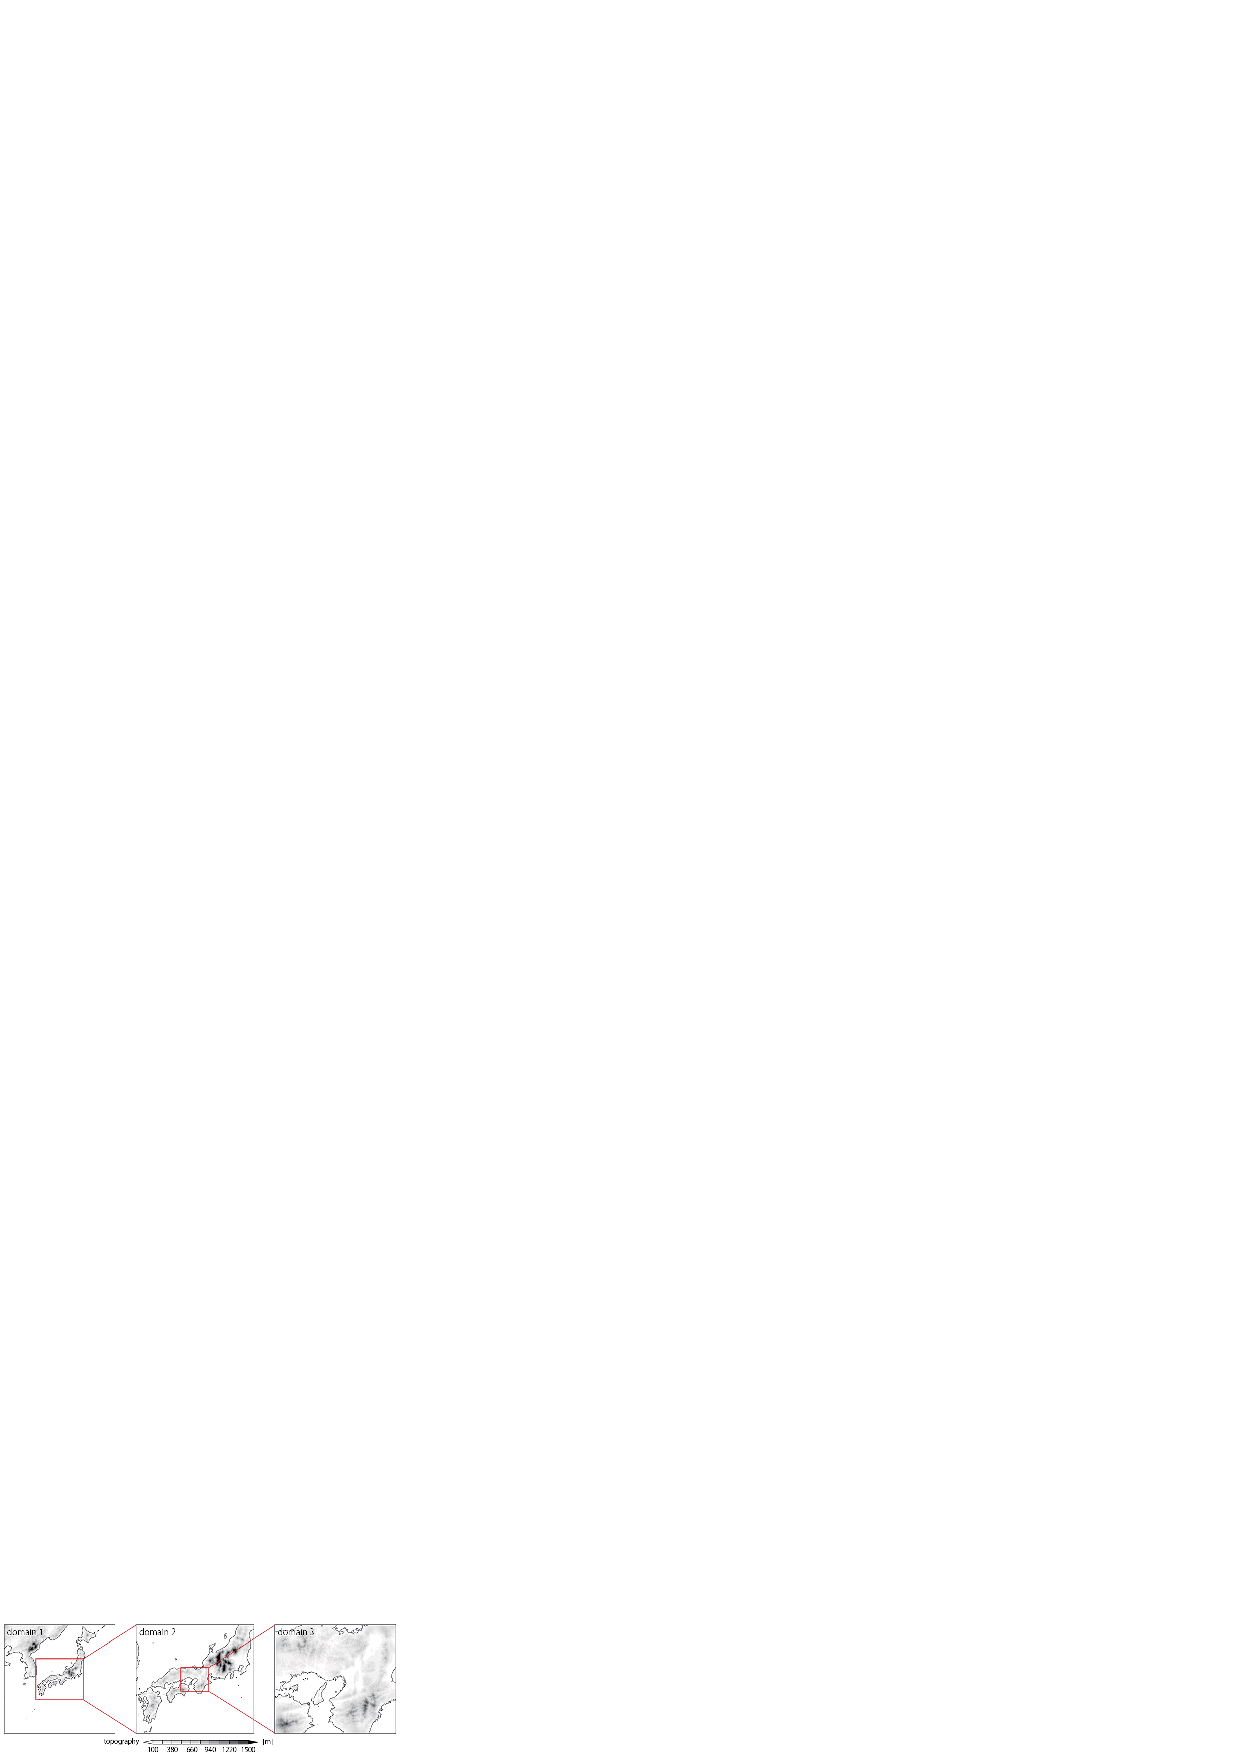
\includegraphics[width=1.0\hsize]{./../../figure/nesting_sample.pdf}\\
  \caption{西日本を対象とした領域ネスティングの例。
    domain 1が最外領域でdomain 3が最内領域である。
    赤い矩形と線は、領域の位置や他の領域との関係を示している。
    水平格子間隔は domain 1 では 7.5 km、domain 2 では 2.5 km、
    domain 3 では 0.5 kmである。}
  \label{fig_nestsample}
\end{center}
\end{figure}

\subsection{\SubsecCopyTopo} \label{subsec:nest_topo}
%------------------------------------------------------
ネスティング実験では、一般的に、親領域と子領域の間で空間解像度が異なるために地形の解像度も異なる。
子領域の緩和領域(第\ref{subsec:buffer}節を参照)では、大気の変数は親領域の変数へとナッジングされる。
2つの領域間で地形の表現が異なると、親領域で計算されるナッジングのための参照データが存在しないことがある。
その場合は外挿により大気データを見積もることになるが、外挿による見積もりの精度が悪いと不整合が生じる。
%
地形の違いによる不整合を回避するために、
\scalerm では「地形コピー」機能を使用することを推奨している。
この機能は、子領域の緩和領域における地形として親領域の地形をコピーする。
この機能を使えば、図\ref{fig_topocopy}に示すように、子領域の緩和領域の地形と
親領域の地形を完全に一致させられる。
さらに、地形の解像度を外側から内側に行くに従って徐々に高めるために、
緩和領域の内側に地形の遷移領域を置く。
地形の遷移領域では、地形は親領域と子領域の地形を重み付けすることで生成される。
地形遷移領域の幅は、デフォルト設定では緩和領域と同じ幅である。
これよりも内側の計算領域では、地形は子領域の地形を与える。
「{\makeconftool}」(第\ref{sec:basic_makeconf}節)を利用する場合は、
地形コピー機能が自動的に適用される。


本節で示す\verb|pp.d0*.conf|ファイルは、サンプル設定ファイル\\
\verb|${Tutorial_dir}/real/sample/USER.online-nesting.sh|を
USER.shに名前を変更して、「{\makeconftool}」を実行することで作成される。
説明を読み進める上で参考にしてもらいたい。
以降は、具体的な設定方法と実行手順を説明する。


\begin{figure}[htb]
\begin{center}
  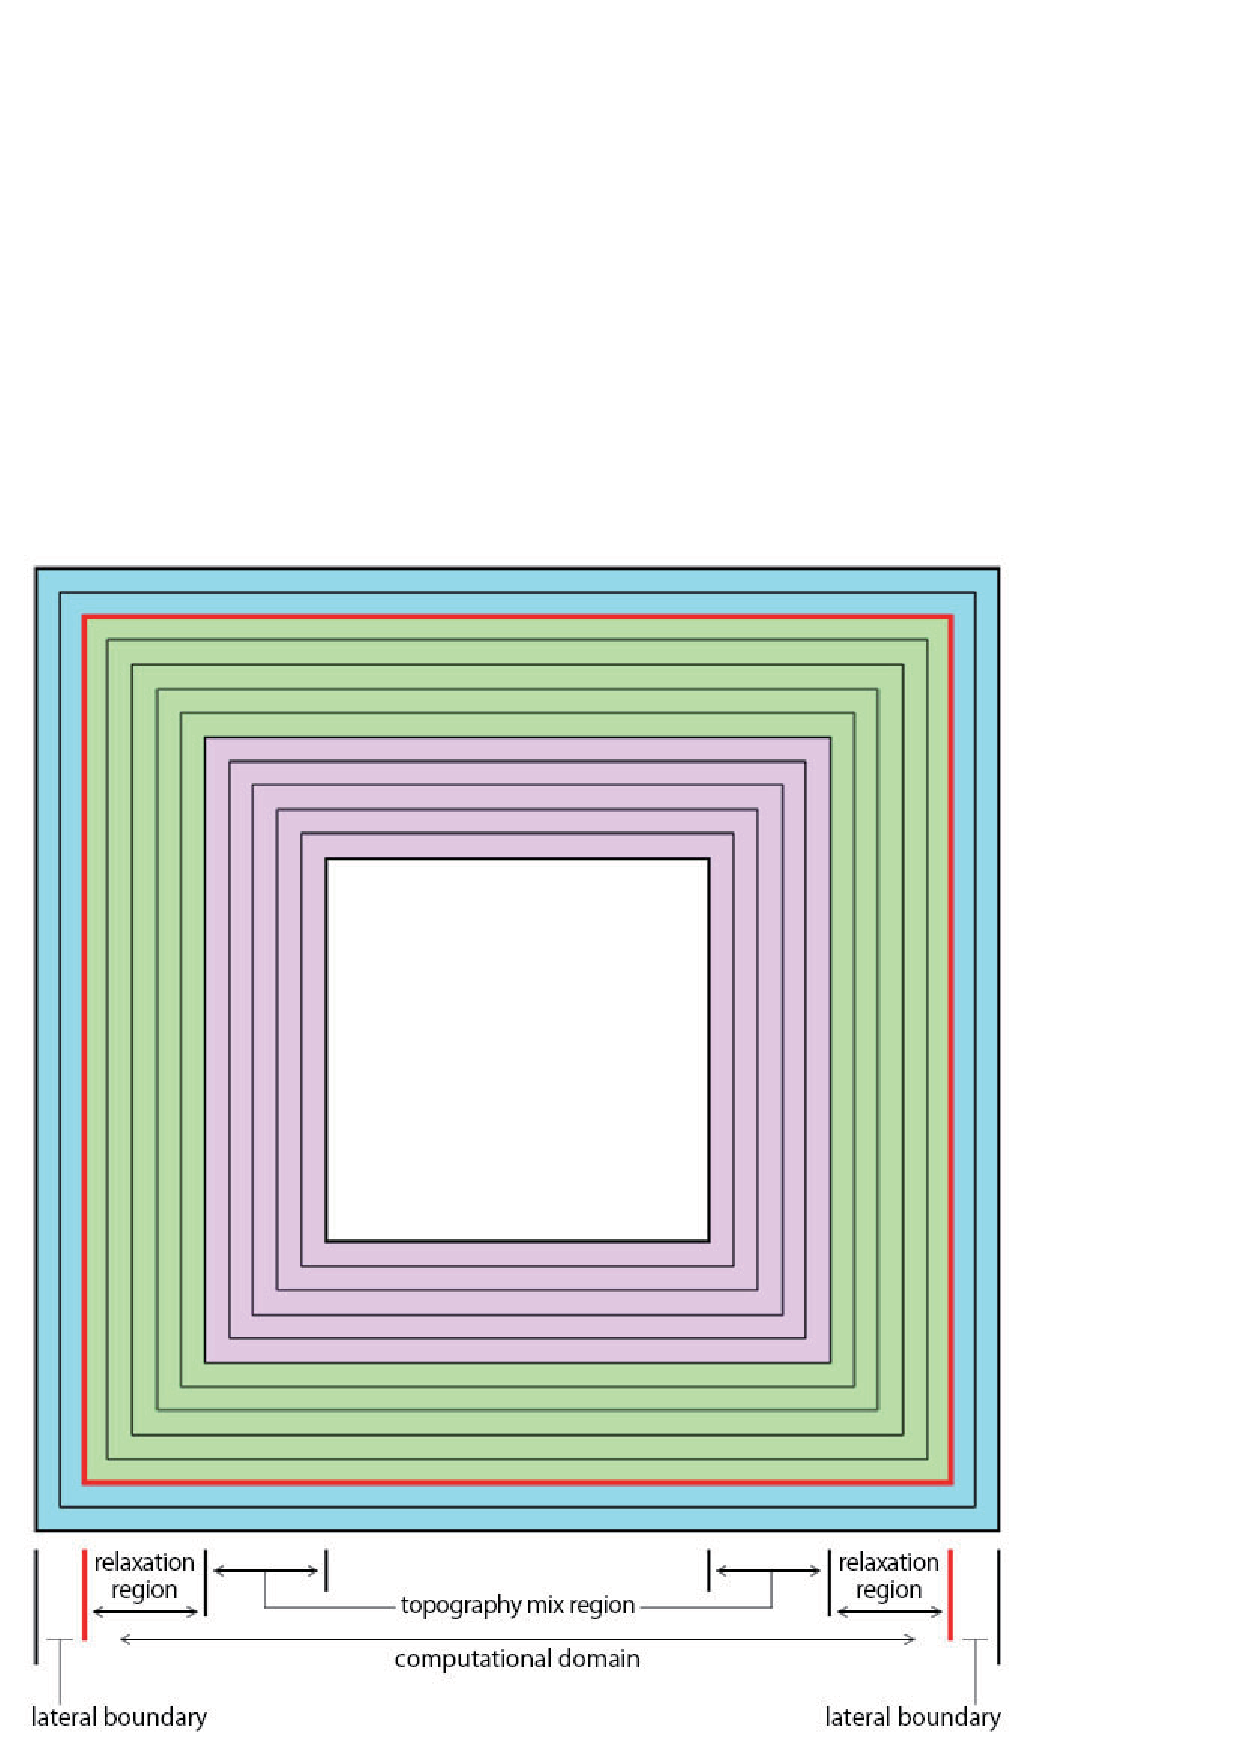
\includegraphics[width=0.4\hsize]{./../../figure/topo_copy.pdf}\\
  \caption{地形コピー機能を適用したときの地形の水平分布。
水色で塗られた最外にある格子は\texttt{HALO}領域であり、
その格子数は水平移流スキームに依存する。
これらの格子は側面境界である。
赤色の線で囲われた部分は、計算領域である。
緑色や桃色の領域はそれぞれ、緩和領域と地形遷移領域である。
最内の白色の領域では、地形は子領域のもとの地形と同じである。
地形遷移領域では、外側から内側にかけて徐々に親領域の地形データから子領域の地形データへ遷移する。}
  \label{fig_topocopy}
\end{center}
\end{figure}


\subsubsection{地形コピー機能の使い方}

親領域の地形データを\verb|scale-rm_pp|で作成する際に、
親領域の大きさを子領域に与えるためのカタログファイルを出力させるには、
下記の設定が\verb|pp.d01.conf|に必要である。\\
\editboxtwo{
\verb|&PARAM_DOMAIN_CATALOGUE|  & \\
\verb| DOMAIN_CATALOGUE_FNAME  = "latlon_domain_catalogue.d01.txt",| & カタログファイルのファイル名\\
\verb| DOMAIN_CATALOGUE_OUTPUT = .true.,| & カタログファイルを出力するか? \\
\verb|/|  & \\
}
その他の設定項目は通常通りで良い。

次に、地形コピー機能で親の地形を用いるために、
子領域に対する\verb|pp.d02.conf|ファイルを以下のように編集する。
ここでは、親領域の地形の出力データが SCALE netCDF フォーマット で \verb|topo_d01.pe***.nc|として保存されていると想定する。その他のフォーマットとしては、GrADS がサポートされている(第\ref{sec:adv_datainput}節)。
\editboxtwo{
\verb|&PARAM_COMM_CARTESC_NEST| & \\
\verb| OFFLINE_PARENT_BASENAME   = "topo_d01", | & 親領域のファイルのベース名 \\
\verb| OFFLINE_PARENT_PRC_NUM_X  = 2,          | & 親領域の\verb|PRC_NUM_X| \\
\verb| OFFLINE_PARENT_PRC_NUM_Y  = 2,          | & 親領域の\verb|PRC_NUM_Y| \\
\verb| LATLON_CATALOGUE_FNAME    = "latlon_domain_catalogue.d01.txt",| & 親領域のカタログファイル  \\
\verb|/| &\\
 & \\
\verb|&PARAM_CNVTOPO|  &\\
\verb|    〜  中略  〜    | & \\
\verb| CNVTOPO_copy_parent     = .true.,| & 地形コピー機能を適用するかどうか\\
\verb|/| &\\
 & \\
\verb|&PARAM_COPYTOPO| & \\
\verb| COPYTOPO_IN_BASENAME   = "topo_d01",| & 親領域の地形データファイルのベース名 \\
\verb| COPYTOPO_IN_FILETYPE   = "SCALE",   | & 親領域の地形データファイルのタイプ名 (SCALE, GrADS) \\
\verb| COPYTOPO_TRANSITION_DX = -1,        | & x方向の遷移域の幅 \\
\verb| COPYTOPO_TRANSITION_DY = -1,        | & y方向の遷移域の幅 \\
\verb| COPYTOPO_ENTIRE_REGION = .false.,|    & 子領域の全域に親領域の地形をコピーするかどうか\\
\verb| COPYTOPO_LINEAR_H      = .true.,|     & \\
\verb|/| & \\
}
\namelist{PARAM_CNVTOPO}の\nmitem{CNVTOPO_copy_parent}を\verb|.true.|とすれば、地形のコピー機能が適用される。
\nmitem{COPYTOPO_ENTIRE_REGION}は、子領域の全域に渡って親領域の地形をコピーするかを決めるオプションである。
これが\verb|.true.|の場合は、子領域の地形は親領域から完全にコピーされる。\\
\nmitem{COPYTOPO_LINEAR_H}は地形の遷移方法を指定するパラメータである。
\nmitem{COPYTOPO_LINEAR_H}が\verb|.true.|であれば子領域と親領域の地形の混合割合が
線形的に変化し、そうでなければ指数関数的に変化する。
遷移領域の幅は\nmitem{COPYTOPO_TRANSITION_DX}や\nmitem{COPYTOPO_TRANSITION_DY}で指定する。
これらの値が負であればデフォルトの設定が適用され、
地形の遷移領域の幅は緩和領域の幅と同じに取られる。


\subsubsection{地形の作成}

地形コピー機能を使用する場合は、
子領域は親領域のカタログファイルを必要とするため、
親領域から順番に地形を作成しなければならない。
領域が3つ以上ある場合は、実行の順番は以下にようになる。

\begin{verbatim}
 $ mpirun -n [プロセス数] ./scale-rm_pp pp.d01.conf
 $ mpirun -n [プロセス数] ./scale-rm_pp pp.d02.conf
 $ mpirun -n [プロセス数] ./scale-rm_pp pp.d03.conf
\end{verbatim}

\subsection{\SubsecOflineNesting} \label{subsec:nest_offline}
%------------------------------------------------------

オフラインネスティング実験を行う上での実験設定の制限事項は、以下の2点である。
\begin{itemize}
 \item 子領域の計算範囲は、親領域の計算範囲の内側に位置している必要がある。
 \item 子領域の積分期間は、親領域の積分期間と同じもしくはそれより短い必要がある。
\end{itemize}

~\\
また、オフライン・ネスティング実験の実行過程は次のようになる。
\begin{enumerate}
 \item 親領域の時間積分計算を行う。
 \item 親領域のhistory出力ファイルを用いて子領域の初期値/境界値を作成する。
 \item 作成した初期値/境界値を用いて子領域の時間積分計算を行う。
\end{enumerate}


以下、この流れに沿って説明を進める。
親領域と子領域それぞれについて、\verb|pp.***.conf|、\verb|init.***.conf|、
そして\verb|run.***.conf|ファイルを事前に作成し、
親領域、子領域ともに地形・土地利用データの作成 (\verb|scale-rm_pp|) が、
親領域については、初期値/境界値データの作成 (\verb|scale-rm_init|) が終わっていることを想定して説明を進める。
ここで説明するオフライン・ネスティング実験の設定を記述した設定ファイルは、
サンプル設定ファイル
\verb|${Tutorial_dir}/real/sample/USER.offline-nesting-parent.sh|および
\verb|${Tutorial_dir}/real/sample/USER.offline-nesting-child.sh|
をそれぞれUSER.shに置き換えて、実験セット一式準備ツールを実行すると作成される。
説明を読み進める上で参考にしてもらいたい。

\subsubsection{親領域の時間積分計算を行う}
基本的には通常のシングルドメインの場合と同じ方法で実行すればよいが、
\verb|run.***.conf|の設定で次の5点に注意する必要がある。

\begin{itemize}
 \item 子領域の計算に必要な変数全てを、親領域の計算時にhistory出力する。
 \item 親領域のhistory出力間隔を適度に細かくとること。
 \item 親領域のhistory出力データは、モデル面のデータを出力すること。
 \item 親領域の計算領域を子領域へ伝える「カタログファイル」(以下参照のこと)を出力する。
 \item (子領域の計算開始時刻が親領域と同じ場合) 親領域のhistory出力データにt=0の値を含めること。
\end{itemize}


この設定を\verb|run.d01.conf|に適用すると下記のようになる。
\textcolor{blue}{青文字}で示した部分が、上記の注意点・変更点に対応する部分である。\\

\noindent {\small {\gt
\ovalbox{
\begin{tabularx}{150mm}{lX}
\verb|&PARAM_DOMAIN_CATALOGUE| & \\
\verb| DOMAIN_CATALOGUE_FNAME  = "latlon_domain_catalogue_d01.txt",| & カタログファイルのファイル名\\
\textcolor{blue}{\verb| DOMAIN_CATALOGUE_OUTPUT = .true.,|} & カタログファイルを出力。\\
\verb|/| &\\
 & \\
\verb|&PARAM_HISTORY| &\\
\verb| HISTORY_DEFAULT_BASENAME  = "history",| & \\
\textcolor{blue}{\verb| HISTORY_DEFAULT_TINTERVAL = 900.D0,|} & historyデータの出力時間間隔。\\
\verb| HISTORY_DEFAULT_TUNIT     = "SEC",|   & \verb|HISTORY_DEFAULT_TINTERVAL|の単位。\\
\verb| HISTORY_DEFAULT_TAVERAGE  = .false.,| & \\
\verb| HISTORY_DEFAULT_DATATYPE  = "REAL4",| & \\
\textcolor{blue}{\verb| HISTORY_DEFAULT_ZCOORD   = "model",|}  & モデル面データを出力。\\
\textcolor{blue}{\verb| HISTORY_OUTPUT_STEP0      = .true.,|}  & t=0の値を出力に含める。 \\
\verb|/| \\
\end{tabularx}
}}}\\

カタログファイルの出力設定を\verb|.true.|にすると、\verb|latlon_domain_catalogue_d01.txt|というカタログファイルが出力される。
実験セット準備ツールを使用した場合、同ファイルがppディレクトリに出力されているので、そちらを参照すること。
この中には、親領域の計算で各MPIプロセスが担当する計算領域の四隅の緯度・経度が記述されている。
\nmitem{HISTORY_DEFAULT_TINTERVAL}はhistoryデータの出力間隔を示し、
子領域の側面境界条件を更新したい時間間隔に設定する。
短い時間間隔でデータを出力する場合には、ディスクの空き容量にも注意が必要である。
その他、\namelist{PARAM_HISTORY}の各項目の詳細は、第\ref{sec:output}節を参照のこと。

また、子領域の初期値/境界値データ作成に必要な変数全てを
\verb|run.d01.conf|ファイルの\namelist{HISTITEM}に追加しておく必要がある。
オフライン・ネスティングに必要な変数は、下記の通りである。
設定が完了したら、\verb|scale-rm|を実行して親領域の時間積分計算を行う。

\begin{alltt}
  T2, Q2, MSLP, DENS, MOMZ, MOMX, MOMY, RHOT
  LAND_SFC_TEMP, URBAN_SFC_TEMP, OCEAN_SFC_TEMP
  OCEAN_ALB_LW, OCEAN_ALB_SW, LAND_ALB_LW, LAND_ALB_SW
  OCEAN_TEMP, OCEAN_SFC_Z0M, LAND_TEMP, LAND_WATER
(親の雲微物理モデルに合わせて出力; 例えばTomita08なら全て)
  QV, QC, QR, QI, QS, QG
(親の雲微物理モデルに合わせて出力; 例えばTomita08なら不要)
  NC, NR, NI, NS, NG
\end{alltt}



%-------------------------------------------------------------
\subsubsection{親領域の出力ファイルを用いて子領域の初期値/境界値を作成する}
次に、計算が終わった親領域のhistoryデータを用いて、子領域の初期値/境界値を作成する。
実行するプログラムは、通常の初期値/境界値作成と同じ \verb|scale-rm_init| だが、
\verb|init.d02.conf|を下記のように設定する。\\

\noindent {\small {\gt
\ovalbox{
\begin{tabularx}{150mm}{lX}
\textcolor{blue}{\verb|&PARAM_NEST|} & \\
\textcolor{blue}{\verb| OFFLINE_PARENT_BASENAME   = "history_d01",|}  & 親領域データのファイル名 \\
\textcolor{blue}{\verb| OFFLINE_PARENT_PRC_NUM_X  = 2,|}  & \verb|run.d01.conf|の\verb|PRC_NUM_X|\\
\textcolor{blue}{\verb| OFFLINE_PARENT_PRC_NUM_Y  = 2,|}  & \verb|run.d01.conf|の\verb|PRC_NUM_Y|\\
\textcolor{blue}{\verb| LATLON_CATALOGUE_FNAME    = "latlon_domain_catalogue_d01.txt",|} & 親領域を実行した時に作成したカタログファイル\\
\textcolor{blue}{\verb|/|} &\\
 & \\
\verb|&PARAM_MKINIT_REAL_ATMOS| &\\
\textcolor{blue}{\verb| NUMBER_OF_TSTEPS    = 25,|}         & historyファイル内の時間ステップ数\\
\verb| FILETYPE_ORG        = "SCALE-RM",| & \\
\verb| BASENAME_ORG        = "history_d01",|  & \verb|run.d01.conf|の\verb|HISTORY_DEFAULT_BASENAME|\\
\verb| BASENAME_BOUNDARY   = "boundary_d01",| &\\
\textcolor{blue}{\verb| BOUNDARY_UPDATE_DT  = 900.D0,|}     & historyファイルの出力時間間隔(単位は\verb|"SEC"|)\\
\verb|/| &\\
 & \\
\verb|&PARAM_MKINIT_REAL_OCEAN| &\\
\textcolor{blue}{\verb| NUMBER_OF_TSTEPS    = 25,|}         & historyファイル内の時間ステップ数\\
\verb| BASENAME_ORG        = "history_d01",|  & \verb|run.d01.conf|の\verb|HISTORY_DEFAULT_BASENAME|\\
\verb| FILETYPE_ORG        = "SCALE-RM",| & \\
\verb|/| &\\
 & \\
\verb|&PARAM_MKINIT_REAL_LAND| &\\
\textcolor{blue}{\verb| NUMBER_OF_TSTEPS    = 25,|}         & historyファイル内の時間ステップ数\\
\verb| BASENAME_ORG        = "history_d01",|  & \verb|run.d01.conf|の\verb|HISTORY_DEFAULT_BASENAME|\\
\verb| FILETYPE_ORG        = "SCALE-RM",| & \\
\verb|/| &\\
\end{tabularx}
}}}\\


\scalerm の出力データから初期値境界値を作成する場合は、
\nmitem{FILETYPE_ORG}に\verb|"SCALE-RM"|を指定する。
\nmitem{BOUNDARY_UPDATE_DT}は、基本的に、親領域の設定ファイル(\verb|run.d01.conf|)の\\
\nmitem{HISTORY_DEFAULT_TINTERVAL}と同じ設定を記述する。
%
\namelist{PARAM_NEST}の項目は、ネスティング実験のための設定項目である。
オフライン・ネスティングでは、\nmitem{OFFLINE_PARENT_BASENAME}に親領域データのファイル名を設定する。
また、\nmitem{OFFLINE_PARENT_PRC_NUM_*} で親領域のプロセス数を設定する。
親領域の設定ファイル(\verb|run.d01.conf|) を参照して正しく設定すること。\\


設定の編集が完了したら、\verb|scale-rm_init|を実行し、子領域の初期値/境界値を作成する。
実行時に下記のようなメッセージが表示されて計算が止まる場合は、
子領域の計算領域が親領域の計算領域の外側に取られている部分がある。
この場合は、各領域の大きさや領域中心の設定を見直す必要がある。\\

\noindent {\small {\gt
\fbox{
\begin{tabularx}{150mm}{l}
\verb|xxx ERROR: REQUESTED DOMAIN IS TOO MUCH BROAD| \\
\verb|xxx -- LONGITUDINAL direction over the limit| \\
\end{tabularx}
}}}\\



\subsubsection{作成した初期値/境界値を用いて子領域の時間積分計算を行う}
初期値/境界値作成が終わったら、子領域の計算 (\verb|scale-rm|) を実行する。
子領域の実行は、通常の現実大気実験と同じである。
1点だけ注意すべき点として、
\verb|run.d02.conf|の\namelist{PARAM_ATMOS_BOUNDARY}の\nmitem{ATMOS_BOUNDARY_UPDATE_DT}が
初期値/境界値作成で使用した親領域のhistoryデータ出力間隔に合っているか確認すること。
現在のところ、この設定に親領域と子領域間で不整合あっても警告やエラーメッセージが発せられないまま、
計算が進み、場合によっては正常終了してしまうため注意が必要である。


\noindent {\small {\gt
\ovalbox{
\begin{tabularx}{150mm}{l}
\verb|&PARAM_ATMOS_BOUNDARY| \\
\verb|     〜 中略 〜|\\
\textcolor{blue}{\verb| ATMOS_BOUNDARY_UPDATE_DT  = 900.D0,|} \\
\verb|/| \\
\end{tabularx}
}}}\\

\noindent
多段のオフライン・ネスティング実験を行いたい場合は、以上の過程を繰り返せばよい。
つまり、子領域として時間積分計算した結果を再度、親領域と見立てて、
さらに内側の孫領域の初期値/境界値作成を行なえばよい。

\subsection{Online Nesting Experiment} \label{subsec:nest_online}
%----------------------------------------------------------

The following two limitations are imposed in carrying out the online nesting experiment:
\begin{itemize}
\item The integration time for the child domain is identical to that for the parent domain.
\item The time step for the parent domain is a multiple of that for the child domain.
\end{itemize}
On the other hand, the configurations of vertical layers, map projections, and the physical scheme do not have to be identical in the parent and the child domains. In the online nesting experiment, computations of all domains are conducted simultaneously. In the current version, \scalerm supports only one-way nesting. The maximum number of domains allowed is 10.

In the online nesting experiment in \scalerm, the time integrations of multiple domains are not serial but parallel. As shown in Fig. \ref{fig_mpisplit}, MPI processes are split into several groups; each group manages a domain and computes it, behaving like an independent model. The configuration file \verb|launch.conf| is needed at execution to boot the multiple domains.

\begin{figure}[tbh]
\begin{center}
  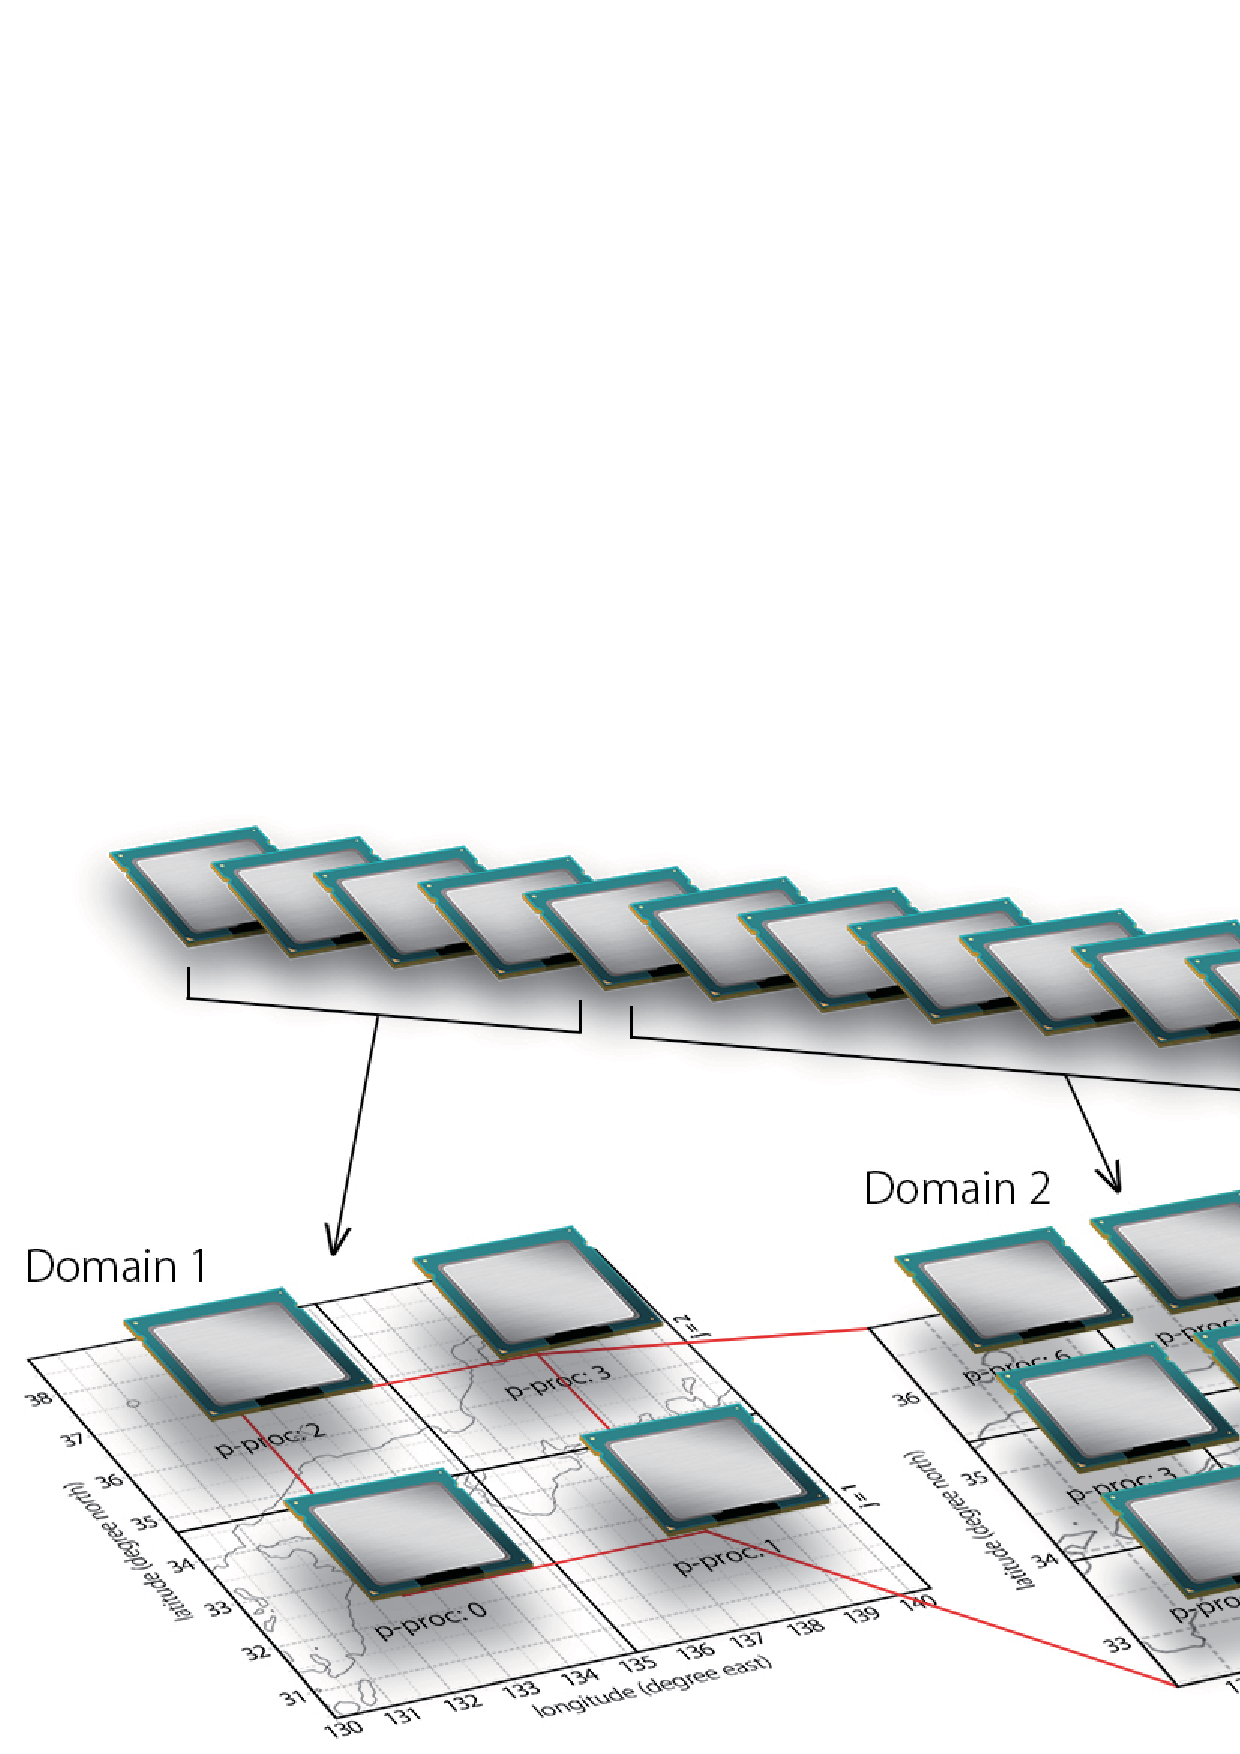
\includegraphics[width=0.8\hsize]{./../../figure/mpisplit_nesting.pdf}\\
  \caption{ MPI process distribution in the online nesting experiment. In this example,   13 processes were launched at the beginning. These processes were distributed appropriately;     4-MPI parallel for $2 \times 2$ in Domain 1 and 9-MPI parallel for $3 \times 3$ in Domain 2 were executed.     MPI communication flowed from Domain 1 to Domain 2.
  }
  \label{fig_mpisplit}
\end{center}
\end{figure}

The following explanation is provided for the most simple case of online nesting, two-domain nesting.
The experimental set described here can be generated by renaming the sample files \\
\verb|${Tutorial_dir}/real/sample/USER.online-nesting.sh|
as USER.sh and conducting ``the supporting tool for the preparation of configuration file'' (refer to Section \ref{sec:basic_makeconf}).
The below explanation assumes that the generations of the topography/land-use data and initial/boundary data for each domain have been completed. The procedures for topography generation are described in Section \ref{subsec:nest_topo}.


\subsubsection{Configurations for Online Nesting}
In the configuration files \verb|run.***.conf| for the parent and child domains, some nesting settings are added to \namelist{PARAM_NEST}:

\noindent {\rm --- Configuration in \verb|run.d01.conf| ---}\\
\editboxtwo{
\verb|&PARAM_NEST|                          & \\
\verb| ONLINE_DOMAIN_NUM        = 1,      | & The domain ID, which is enumerated from the outermost one as 1.\\
\verb| ONLINE_IAM_PARENT        = .true., | & \\
\verb| ONLINE_IAM_DAUGHTER      = .false.,| & \\
\verb| ONLINE_BOUNDARY_USE_QHYD = .true., | & \\
\verb| ONLINE_AGGRESSIVE_COMM   = .true., | & \\
\verb|/| \\
}
~\\
\noindent {\rm --- Configuration in \verb|run.d02.conf| ---}\\
\editboxtwo{
\verb|&PARAM_NEST| & \\
\verb| ONLINE_DOMAIN_NUM        = 2,      | & The domain ID, which is enumerated from the outermost one as 1.\\
\verb| ONLINE_IAM_PARENT        = .false.,| & \\
\verb| ONLINE_IAM_DAUGHTER      = .true., | & \\
\verb| ONLINE_BOUNDARY_USE_QHYD = .true., | & \\
\verb| ONLINE_AGGRESSIVE_COMM   = .true., | & \\
\verb|/| \\
}

\nmitem{ONLINE_DOMAIN_NUM} is the ID number of the domain, which is enumerated from the outermost domain to the innermost.
In above example, the ID numbers of the parent and child domains are 1 and 2, respectively.\\
\nmitem{ONLINE_IAM_PARENT} and \nmitem{ONLINE_IAM_DAUGHTER} specify whether each domain has its parent domain and child domain or not.
If \nmitem{ONLINE_IAM_PARENT} $=$ \verb|.true.| in the $N$th domain, the calculation data in the $N$th domain is transferred to the child domain with the domain number of $N+1$.
If \nmitem{ONLINE_IAM_DAUGHTER} $=$ \verb|.true.|, then boundary data in the $N$th domain is received from the parent with the domain number of $N-1$.
The outermost domain plays a role only in the parent domain, whereas the innermost domain is involved only in the child domain.
Since the intermediate domains are involved in both the parent and child domains, both \nmitem{ONLINE_IAM_PARENT} and \nmitem{ONLINE_IAM_DAUGHTER} are \verb|.true.|.
Table \ref{tab:triple_nested} gives the configuration for an $N$-domain nesting experiment.

\begin{table}[htb]
\begin{center}
\caption{A configuration for $N$-domain nesting}
\begin{tabularx}{150mm}{|l|l|l|X|} \hline
 \rowcolor[gray]{0.9} domain & \verb|ONLINE_DOMAIN_NUM| & \verb|ONLINE_IAM_PARENT| & \verb|ONLINE_IAM_CHILD|\\ \hline
 the outermost domain & 1            & .true.  & .false. \\ \hline
 intermediate domains & 2 -- ($N-1$) & .true.  & .true. \\ \hline
 the innermost domain & $N$          & .false. & .true. \\ \hline
\end{tabularx}
\label{tab:triple_nested}
\end{center}
\end{table}


\nmitem{ONLINE_BOUNDARY_USE_QHYD} specifies whether water condensation is used for the boundary condition. When the boundary condition is generated from external input data, water condensations are not usually employed. However, in the nesting experiment, water condensation calculated in the parent domain can be used for the boundary condition of the child domain because there is often no difference in physical schemes between the two domains.
%, and the resolution of both are similar.
The delay in the generation of clouds and rain, possible to have the influence on interior target domain, is expected to be suppressed by this remedy.

\subsubsection{Configuration of Launcher}
\label{subsubsec:launch}
The online nesting experiment requires the configuration of the launch file \verb|launch.conf|
other than \verb|run.***.conf|.
\editboxtwo{
\verb|&PARAM_LAUNCHER|      & \\
\verb| NUM_DOMAIN  = 2,|    & number of domains\\
\verb| PRC_DOMAINS = 4, 16,| & MPI processes used for each domain (as many domains as necessary)\\
\verb| CONF_FILES  = run.d01.conf, run.d02.conf,| & The configuration files for each domain (as many domains as necessary)\\
\verb|/|& \\
}
\nmitem{CONF_FILES} must correspond to \nmitem{PRC_DOMAINS} in order.
The above case means that
the run is executed by
the 4-MPI parallel for the parent domain 
and the 16-MPI parallel for the child domain;
each number of processes in the launch file 
must correspond to the total number of MPI processes ( \verb|PRC_NUM_X|$\times$\verb|PRC_NUM_Y| )
specified in each configuration file \verb|run.***.conf|.

At execution, the total number of MPI processes is given, which different from that in the case of single-domain execution. For example, 20 processes are specified in the above case.
\begin{verbatim}
 $ mpirun  -n  [number of processes]  ./scale-rm  launch.conf
\end{verbatim}

When multiple domain calculations are executed at the same time,
the different file names must be used for input/output files
among domains to avoid any confusion.
For example, the configuration files prepared by the 
``the making tool for the complete settings of the experiment''
use \verb|history_d01.pe***.nc, history_d02.pe***.nc| for the file name of history output.

The calculation may sometimes abort, outputting the message below. This is the error message, meaning that the domain of computation of the child  is larger than that of the parent domain. If such a message appears, retry creating the topography, the land-use data, and the initial/boundary data, and confirm again whether the configurations are correct:
\msgbox{
  \verb|ERROR [COMM_CARTESC_NEST_domain_relate] region of daughter domain is larger than that |\\
  \verb| of parent| \\
}


\subsubsection{Guideline for Distribution of MPI Processes}
%-------------------------------------------------------------------------

As shown in Fig. \ref{fig_mpisplit}, no MPI process is shared between the multiple domains in the online nesting experiment. In other words, each MPI process takes charge of a part of a specific domain. Therefore, the user should determine how many MPI processes to allocate to each domain. When this allocation is not appropriate, a long waiting time is incurred. To avoid this situation, it is reasonable to allocate processes so that the magnitude of time integrations for each process is as similar as possible among processes\footnote{More accurately, floating-point operations should be estimated.}. Here, the magnitude of time integration, i.e., computational effort, is defined as the product of the number of grids and time steps.

Let us consider $N$-domain nesting. The number of grids in the x, y, and z directions in n-th domain are denoted by
\verb|IMAX_n|, \verb|JMAX_n|, and \verb|KMAX_n|, respectively.
\verb|DT_n| is the time interval \nmitem{TIME_DT} in the n-th domain.
Using the time-step of the outermost domain (n=1) \verb|DT_1| as a benchmark,
the necessary number of time steps in the n-th domain is estimated as:
\begin{eqnarray}
 \verb|TSTEP_n| = \verb|DT_1| / \verb|DT_n|  \nonumber
\end{eqnarray}
The calculation for the n-th domain is derived by multiplying the number of grids as
\begin{eqnarray}
 \verb|OPR_n| = \verb|IMAX_n| \times \verb|JMAX_n| \times \verb|KMAX_n| \times \verb|TSTEP_n| \nonumber
\end{eqnarray}
Therefore, the standard number of processes allocated to the n-th domain is estimated as
\begin{eqnarray}
 \verb|MPI_total| \times \frac{ \texttt{OPR\_n} }{ \sum_{m=1}^N \texttt{OPR\_m} },
\end{eqnarray}
where \verb|MPI_total| is the total number of MPI processes.

The number of processes distributed along the x and y directions \nmitem{PRC_NUM_X, PRC_NUM_Y} can be arbitrarily decided.
It is recommended to configure them so that the difference between \verb|IMAX| and \verb|JMAX| is as small as possible. This is because such a configuration can reduce the area of the halo. As a result, high computational performance can be obtained\footnote{Note that in case of hybrid parallelization used together with thread parallelism,  e.g., in the K computer, it is necessary to take a larger number of grids along the y-axis than the x-axis to minimize computational imbalance between threads.}. 


In the above explanation, only the number of grids and time steps are considered. However, in actual calculations such as nesting simulation in real atmospheric experiment, the time interval for each physical process, and intra-domain and inter-domain communications affect the elapsed time. In the online nesting configuration, because the calculation in the innermost domain is largest in general, it is reasonable to distribute MPI processes so that waiting time caused by MPI communications is minimized in the innermost domain.  In case of large-scale computations, long integration and many ensemble simulations, it is recommended to tune for the distribution of processes following the above rough estimation.


\section{How to run bulk job} \label{sec:bulkjob}
%====================================================================================

 \scalerm has a function for bulk jobs that allows multiple independent jobs be handled simultaneously. This function is useful for the parameter-sweep experiment, the ensemble experiment in different initial conditions, the time-slice climate simulation, and so on.

The bulk job function can be used not only for model simulation (\verb|scale-rm|), but also for the generation of topographical data, land-use data, and initial/boundary data. Note that the generation of topographical/land-use data by this function is limited to the case without a topography copy function (See \ref{subsec:nest_topo}).

In the following explanation, an independent execution in the bulk job is called a ``sub-job.'' Three two-domain nesting experiments are taken up as an example. This set of experiments is imaged as three sub-jobs with different integration periods and centers of calculation domain. \nmitem{NUM_DOMAIN, PRC_DOMAINS, CONF_FILES} in \namelist{PARAM_LAUNCHER} in the file \verb|launch.conf| (refer to Section \ref{subsubsec:launch} ) must be the same in all configurations. The other settings, such as integration time, the scheme used, and the number of grids per MPI process, do not need to be the same among the sub-jobs.

\begin{figure}[t]
\begin{center}
  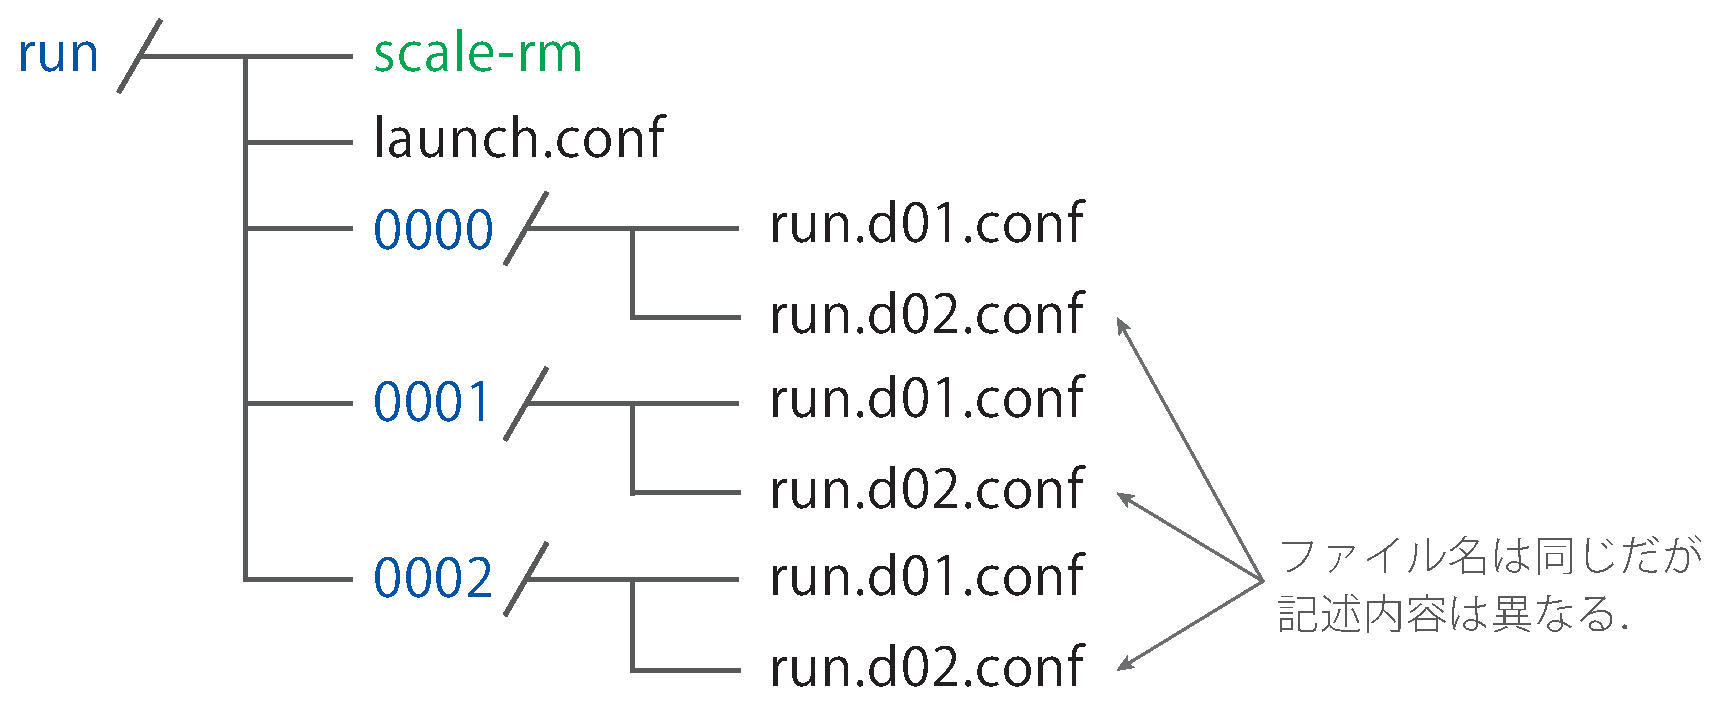
\includegraphics[width=0.6\hsize]{./figure/bulkjob_directory_structure.eps}\\
  \caption{Structure of directories at the bulk job execution of \scalerm.
Numbers such as ``0000'' are the directory names corresponding to job number, and called the job directory.   All necessary configuration files must be prepared in each job directory.
}
  \label{fig_bulkjob}
\end{center}
\end{figure}

Since the bulk job function is an extension of the division and redistribution of MPI processes used in online nesting, file \verb|launch.conf| is required to launch the job. Even in case online nesting and bulk job functions are used together, only one file \verb|launch.conf| is prepared.
Below is an example of such a case.
\editboxtwo{
\verb|&PARAM_LAUNCHER|       & \\
\verb| NUM_BULKJOB = 3,|     & number of sub-jobs\\
\verb| NUM_DOMAIN  = 2,|     & number of nesting domains\\
\verb| PRC_DOMAINS = 9, 36,|  & \\
\verb| CONF_FILES  = run.d01.conf, run.d02.conf,| & \\
\verb|/| \\
}
It is sufficient to add item \nmitem{NUM_BULKJOB} to the \verb|launch.conf|. The other configurations are similar to those in Section \ref{subsubsec:launch}. In case of a single-domain experiment (no nesting), specify \nmitem{NUM_DOMAIN} $=$ 1 and assign a file name to \nmitem{CONF_FILES}.

Prior to the execution of bulk jobs, prepare as many directories as the number of jobs, which are called ``sub-directories.'' As in Fig. \ref{fig_bulkjob}, these correspond to \verb|0000/  0001/  0002/|. The directory name is assigned as a four-digit number starting from zero. In each directory, all the necessary files (configuration files, input files, and output directories) must be prepared.
Note than the path to directoies or files specified in the configuration files must be correctly set up as explained below.
An excerpt of \verb|run.d01.conf| for job \verb|0000| are as follows:
\editbox{
\verb|&PARAM_IO| \\
\verb| IO_LOG_BASENAME = "0000/LOG_d01",| \\
\verb|/| \\
 \\
\verb|&PARAM_RESTART| \\
\verb| RESTART_OUTPUT       = .true.,| \\
\verb| RESTART_OUT_BASENAME = "0000/restart_d01",| \\
\verb| RESTART_IN_BASENAME  = "../init/0000/init_d01_00013046400.000",| \\
\verb|/| \\
 \\
\verb|&PARAM_TOPO| \\
\verb| TOPO_IN_BASENAME = "../pp/0000/topo_d01",| \\
\verb|/| \\
 \\
\verb|&PARAM_LANDUSE| \\
\verb| LANDUSE_IN_BASENAME = "../pp/0000/landuse_d01",| \\
\verb|/| \\
 \\
\verb|&PARAM_ATMOS_BOUNDARY| \\
\verb|     〜 ... 〜|\\
\verb| ATMOS_BOUNDARY_IN_BASENAME    = "../init/0000/boundary_d01",| \\
\verb|     〜 ... 〜|\\
\verb|/| \\
 \\
\verb|&PARAM_HISTORY| \\
\verb| HISTORY_DEFAULT_BASENAME  = "0000/history_d01",| \\
\verb|     〜 ... 〜|\\
\verb|/| \\
}

As shown in Fig. \ref{fig_bulkjob}, job directories exist in the same hierarchy as the directory of the executable binary. That is, a configuration file exists under each job directory, whereas the input files and the output directories must be described as relative paths from the location of  the executable binary. The output directory in the 0000 experiment is \verb|0000/| and the name of output files are as \verb|0000/***|. {\color{blue}{ Note that when the file name is common to all experiments without job directory settings, the output is written to the same file, and the data disappear as a result.
}}


%% バルクジョブの実行は、全サブジョブを実行するのに必要なMPIプロセス数を指定し、
%% \begin{verbatim}
%%  $ mpirun  -n  135  ./scale-rm  launch.conf
%% \end{verbatim}
%% と行う。例では、一つのサブジョブあたり、$9 + 36 = 45$プロセス使用し、全体で3つのジョブを実行するので、
%% 総計で135プロセスを必要とする。
%% %
%% 実行すると得られるLOGファイルに、MPIプロセスを分割した時の情報が示されている。
%% LOGファイルを開くと、最初の「SCALEロゴ」のあとに下記のようなメッセージが出力される。
%% 下記、ドメイン1のプロセス0からの出力例である。\\

At the execution of bulk jobs, the total number of MPI processes is specified as 

\begin{verbatim}
 $ mpirun  -n  135  ./scale-rm  launch.conf
\end{verbatim}
In this example, the number of processes per sub-job is 45 ($=9 + 36$) and the total number of processes used for three sub-jobs is 135. The message providing information regarding the division of MPI processes is written to the LOG files after the \scalelib logo. The following example is the log output for process 0 of Domain 1:
\msgboxtwo{
\verb| ++++++ Start MPI|  & \\
\verb| *** UNIVERSAL_COMM_WORLD        :        0| &; different by execution environment\\
\verb| *** total process [UNIVERSAL]   :      135| &\\
\verb| *** my process ID [UNIVERSAL]   :       36| &\\
\verb| *** master rank?  [UNIVERSAL]   :        F| &\\
\verb| *** GLOBAL_COMM_WORLD           :        3| &; different by execution environment \\
\verb| *** total process [GLOBAL]      :       45| &\\
\verb| *** my process ID [GLOBAL]      :       36| &\\
\verb| *** master rank?  [GLOBAL]      :        F| &\\
\verb| *** LOCAL_COMM_WORLD            :        4| &; different by execution environment\\
\verb| *** total process [LOCAL]       :        9| &\\
\verb| *** my process ID [LOCAL]       :        0| &\\
\verb| *** master rank?  [LOCAL]       :        T| &\\
\verb| *** ABORT_COMM_WORLD            :        0| &\\
\verb| *** master rank ID [each world] :        0| &\\
&\\
}
The items belonging to \verb|[LOCAL]|, \verb|[GLOBAL]|, and \verb|[UNIVERSAL]| are the descriptions, respectively, of the process group in the domain, the nesting group, and the job group. The \verb|UNIVERSAL| group includes the \verb|GLOBAL| group and the \verb|GLOBAL| group includes the \verb|LOCAL| group. \verb|total process| represents the total number  of processes in each group and \verb|my process ID| the ID of the process in the group.

It can be confirmed in this case that 1) since \verb|total process [UNIVERSAL]| is 135, all these processes are completed executed; 2) since \verb|total process [GLOBAL]| is 45, these 45 processes are used in a sub-job; 3) since this example is the log file for Domain 1,  \verb|total process [LOCAL]| is correctly described as 9. If you see the log message for Domain 2,  it is 39. \verb|my process ID [UNIVERSAL]|  is the process number  corresponding to the LOG and history files. Since this notation is the same as in the abnormal completion of execution, you can immediately recognize the processes in which errors occur during the execution of the sub-jobs. \textcolor{blue}{Note that in the current version, all jobs are forcibly terminated if a job is abnormally finished.} 


%%%%%%%%%%%%%%%%%%%%%%%%%%%%%%%%%%%%%%%%%%%%%%%%%%%%%%%%%%%%%%%%%%%%%%%%%%%%%%%%%%%%%%


\section{\SecMakeconfTool} \label{sec:basic_makeconf}
%------------------------------------------------------

実験のための設定ファイル\verb|***.conf|は、
\verb|pp, init, run|用にそれぞれ用意する必要がある。
ネームリストのいくつかの項目はこれらの設定ファイル間で共通でなければならず、
不整合がある場合にはモデルは適切に動かない。
そのような失敗を避けるために、設定ファイルの準備を行うための便利な補助ツール(\makeconftool)を、下記のように用意している。
\begin{verbatim}
 $ cd ${Tutorial_DIR}/real/
 $ ls
    Makefile
      : 実験に必要なファイルを生成するためのMakefile
    README
      : README ファイル
    USER.sh
      : 設定を指定するためのシェルスクリプト
    config/
      : 各々の設定に対する設定ファイル (ユーザは書き換える必要はない)
    sample
      : USER.sh のサンプルスクリプト
    data
      : 現実大気実験のチュートリアル用のファイル
    tools
      : 現実大気実験のチュートリアル用のファイル。FNL データを grib 形式からバイナリ形式に変換するときに使われる。
\end{verbatim}
本ツールの初期設定は現実大気実験のチュートリアルに合わせているが、
ユーザーは\verb|USER.sh|で設定を変更できる。

\verb|sample/| ディレクトリの下に、いくつかのサンプルスクリプトを典型的な設定例として用意している。
必要に応じて、これらの内容を\verb|USER.sh|にコピーして使用すると良いだろう。
\begin{verbatim}
 $ ls sample/
   USER.default.sh
     : 現実大気実験のチュートリアル用の USER.sh と同じ(シングルドメイン用)。
   USER.offline-nesting-child.sh
     : オフライン・ネスティングによる実験の子領域用。
   USER.offline-nesting-parent.sh
     : オフライン・ネスティングによる実験の親領域用。
   USER.online-nesting.sh
     : オンライン・ネスティング用。
\end{verbatim}


\subsubsection{ツールの使い方}

使い方はREADMEに書かれているように、以下の通りである。
\begin{enumerate}
  \item ユーザが希望する実験設定に従って、\verb|USER.sh|を編集する。
  \item \verb|make|コマンドを実行する。
\end{enumerate}
これにより、\verb|experiment|ディレクトリ以下に実験に必要な設定ファイル一式が作成される。

\verb|USER.sh|の設定は現実大気のチュートリアルに対する設定になっているので、
以下のようにチュートリアル設定を別ファイルとして残しておくことを勧める。
\begin{verbatim}
 $ mv experiment/ tutorial/
     : (既にexperimentディレクトリがある場合)
 $ cp USER.sh USER_tutorial.sh
 ... USER.shを編集 ...
 $ make
 $ cp -rL experiment 任意の場所/
     : 「任意の場所」は、任意の場所にあるディレクトリの名前を意味する。
\end{verbatim}


\subsubsection{\texttt{USER.sh}の編集}

%まず、サンプルプログラムの中、最も想定する実験設定に近いスクリプトを
%\verb|USER.sh| に上書きコピーする。
スクリプトファイルの最初の方に、ドメインの数を指定する\verb|NUM_DOMAIN|がある。
その下には、スクリプトが生成する設定ファイルに指定される項目が並んでいて、
これらの項目を適切に変更すると良いだろう。
項目の後に「\verb|# required parameters for each domain|」というコメントが存在する場合には、
項目の値をドメインの数だけスペースで区切って書く。
項目の値の数と\verb|NUM_DOMAIN|で設定したネスティングドメインの数が異なれば、
実験用のファイル一式が作成されないことに注意が必要である。
\verb|USER.sh|にない項目については、\verb|experiment|ディレクトリ以下に作成された設定ファイルを
直接編集されたい。

\section{Setting the common components} \label{sec:common}
%------------------------------------------------------

\subsection{Calendar} \label{subsec:calendar}
%------------------------------------------------------

The calendar is specified in \namelist{PARAM_CALENDAR} in files \verb|init.conf| and \verb|run.conf|.
Gregorian calendar is used in default.

\editboxtwo{
\verb|&PARAM_CALENDAR             | & \\
\verb| CALENDAR_360DAYS = .false. | & ; Whether 12x30 days calendar is used \\
\verb| CALENDAR_365DAYS = .false. | & ; Whether leap year is considered \\
\verb|/                           | & \\
}

\noindent
The setting of the calendar affects calculation of solar zenith angle.
It is calculated so that length of one year and the full circle of the ecliptic match.
Note that the external data in the different calendar should not be read.

When \nmitem{CALENDAR_360DAYS} is \verb|.true.|,
the calendar that one year is 12 months and one month is 30 days, is set.
%
When \nmitem{CALENDAR_365DAYS} is \verb|.true.|,
the Gregorian calendar is used without leap year.


\chapter{詳細説明 (応用編)} \label{chap:detail}
%-------------------------------------------------------------------------------
\section{What is \scalenetcdf File?} \label{sec:netcdf}
%-------------------------------------------------------------------------------

In this section, \scalenetcdf file, which \scalelib directly reads from and writes in, is explained.
\scalelib employs \netcdf (network Common Data Format) as data file format.
\Netcdf is a software developed by Unidata (\url{http://www.unidata.ucar.edu/}),
and it enables us to generate files with self-describing and machine-independent data format;
for example, the former has a merit to describe variables along with their axis variables in a file and
the latter has a merit to treat data without worry which endian is used.
Based on the above virtue, \scalelib has particular convention ( \scalenetcdf convention ).
It is mostly following the CF conventions \\ (\url{http://cfconventions.org}).


\subsection{Global Attributes} \label{sec:global_attr}
\scalenetcdf file contains information about data contained in the file,
such as those with regards to spatial decomposition as ``Global Attributes'' (Table \ref{table:netcdf_global_attrs}).

\begin{table}%[bth]
\begin{center}
  \caption{Global attributes in \scalenetcdf file}
  \label{table:netcdf_global_attrs}
  \begin{tabularx}{150mm}{p{50mm}XX} \hline
    Name        & Description                 & Remarks \\ \hline \hline
    title       & Brief description of data   & Value of \nmitem{FILE_HISTORY_TITLE} in \namelist{PARAM_FILE_HISTORY} \\
    source      & Name of the source software & Value of \nmitem{FILE_HISTORY_SOURCE} in \namelist{PARAM_FILE_HISTORY} for history files and \nmitem{H_SOURCE} in \namelist{PARAM_IO} for other files\\
    institution & Data author                 & Value of \nmitem{FILE_HISTORY_INSTITUTION} in \namelist{PARAM_FILE_HISTORY} for history files and \nmitem{H_INSTITUTE} in \namelist{PARAM_IO} for other files\\
    rankid      & Rank id of MPI process      & \verb|PRC_myrank| in the model \\
    Conventions & CF convention version       & ``CF-1.6'' for version 5.3 \\
    grid\_name  & Grid type                   & ``cartesC'' for \scalerm \\
    scale\_cartesC\_prc\_rank\_[xy]           & Mapping index of the 2D decomposition      & Equal to \verb|PRC_2Drank(PRC_myrank, i)| variable in the model (i=1 for x and 2 for y)\\
    scale\_cartesC\_prc\_num\_[xy]            & Number of the 2D decomposition             & ~\nmitem{PRC_NUM_X}, \nmitem{PRC_NUM_Y} in the model \\
    scale\_cartesC\_prc\_periodic\_[zxy]      & Whether the boundary condition is periodic & \verb|.false.| and \verb|.true.|\ They correspond to \nmitem{PRC_PERIODIC_X}, \nmitem{PRC_PERIODIC_Y} in the model\\
    scale\_atmos\_grid\_cartesC\textbackslash \ ~~\_index\_[ij]maxg  & Number of the grids in the global domain               & ~\nmitem{IMAXG}, \nmitem{JMAXG} in the model \\
    scale\_atmos\_grid\_cartesC\textbackslash \ ~~\_index\_kmax      & Number of the vertical layer for the atmospheric model & ~\nmitem{KMAX} in the model \\
    scale\_ocean\_grid\_cartesC\textbackslash \ ~~\_index\_kmax      & Number of the vertical layer for the ocean model       & ~\nmitem{OKMAX} in the model \\
    scale\_land\_grid\_cartesC\textbackslash \ ~~\_index\_kmax       & Number of the vertical layer for the land model        & ~\nmitem{LKMAX} in the model \\
    scale\_urban\_grid\_cartesC\textbackslash \ ~~\_index\_kmax      & Number of the vertical layer for the urban model       & ~\nmitem{UKMAX} in the model \\
    scale\_atmos\_grid\_cartesC\textbackslash \ ~~\_index\_[kij]halo & Number of halo grids                                   & ~\nmitem{KHALO}, \nmitem{IHALO}, \nmitem{JHALO} in the model \\
    Calendar    & Calendar type                            & ~\nmitem{PARAM_CALENDAR} in the model \\
    time\_units & Unit of time & \\
    time\_start & Start time   & \\ \hline
    \multicolumn{3}{l}{Refer Section \ref{sec:output} for \nmitem{HISTORY_TITLE, HISTORY_SOURCE, HISTORY_INSTITUTION},} \\
    \multicolumn{3}{l}{Section \ref{sec:domain}       for \nmitem{PRC_NUM_X, PRC_NUM_Y, PRC_PERIODIC_X, PRC_PERIODIC_Y} and} \\
    \multicolumn{3}{l}{\nmitem{KMAX, IMAXG, JMAXG}, and Section \ref{subsec:calendar} for \nmitem{PARAM_CALENDAR}.} \\ \hline
  \end{tabularx}
\end{center}
\end{table}



\subsection{Data in the Halo Region}

Whether the file 
contains the data in the halo region
depends on the type of file and its configuration.
Note that the halo region that we define here means the halo in the whole calculation region,
not the halo in each of local regions.

For the initial (or restart) and boundary data files, 
the halo data is contained if the lateral boundary conditions are not periodic 
(\nmitem{PRC_PERIODIC_X}, \nmitem{PRC_PERIODIC_Y} = .false. in \namelist{PARAM_PRC_CARTESC}) 
or the single file I/O (Section \ref{subsec:single_io}) is used (\nmitem{FILE_AGGREGATE}=.true. in \namelist{PARAM_FILE}),
otherwise it is not.

On the other hand,
for the history data file, 
the halo data is contained 
only when the lateral boundary conditions are not periodic
and \nmitem{FILE_HISTORY_CARTESC_BOUNDARY}=.true. \\
in \namelist{PARAM_FILE_HISTORY_CARTESC},
otherwise it is not. Refer Section \ref{sec:output} for detail.


\subsection{Axis Variables}
\scalenetcdf file contains axis data.
All the axis variables have 
``long\_name'' and ``units'' attributes,
which describe description and unit of the variable, respectively.
In addition, x, y, xh, and yh variables 
have attributes for the total number of grids in the whole domain (``size\_global''),
the start index in the total grid of data in the file (``start\_global''),
the number of the halo grids at the begin and end in the whole data (``halo\_global''),
and the number of the halo grids of data in the file (``halo\_local'').

Table \ref{table:netcdf_axes} shows list of the axis data.
The coordinate variables have their own dimension; their variable names are the same as their dimension names.
%The other axis variables use some dimensions of coordinate variables.
The variables with lower-case name are mainly used in the file, 
while those with the upper-case name describe axes in simulation.
Figure \ref{fig:netcdfhorizontalcoordinate} and \ref{fig:netcdfverticalcoordinate} show 
the horizontal and vertical locations of coordinate variables,
respectively.
Refer to them with Table \ref{table:netcdf_axes} at the same time.

The area and volume data of the grids are also in the file as ``cell\_area**'' and ``cell\_volume**'', respectively.
The ``cell\_measures'' attribute of each variables specifies the corresponding area or volume data.

The map projection data is contained as a non-dimensional variable whose name is specified by ``grid\_mapping'' attribute of the variables.

The information of relationship with the staggered grids is contained as an attribute and a non-dimensional variable, based on SGRID conventions (\url{https://github.com/sgrid/sgrid}).
The non-dimensional variable's name is specified by the ``grid'' attribute of each variable.

In the file, there are also the surface elevation data and land mask data as ``topo'' and ``lsmask'', respectively.



\begin{longtable}{l|l}
  \caption{Axis data in \scalenetcdf .}
  \label{table:netcdf_axes} \\ \hline
  \endfirsthead
  \multicolumn{2}{l}{\small\it Cont.} \\ \hline
%  & name & description \\ \hline \hline
  \endhead
  \hline
  \endfoot
  \multicolumn{2}{l}{Coordinate variables}\\ \hline
name & description \\ \hline \hline
\multicolumn{2}{c}{Horizontal axis \& time axis: Common}\\ \hline
x        & full level position in x-direction of the data in the file \\
x\_bnds  & full level cell boundary in x-direction of the data in the file \\
xh       & half level position in x-direction of the data in the file \\
xh\_bnds & half level cell boundary in x-direction of the data in the file \\
y        & full level position in y-direction of the data in the file \\
y\_bnds  & full level cell boundary in y-direction of the data in the file \\
yh       & half level position in y-direction of the data in the file \\
yh\_bnds & half level cell boundary in y-direction of the data in the file \\
time       & time information \\ \hline
time\_bnds & time boundary information \\ \hline
CX  & full level grid position in x-direction for the local region (inc. halo grids) \\
FX  & half level grid position in x-direction for the local region (inc. halo grids) \\
CDX & full level grid spacing  in x-direction (inc. halo grids) \\
FDX & half level grid spacing  in x-direction (inc. halo grids) \\
CY  & full level grid position in y-direction for the local region (inc. halo grids) \\
FY  & half level grid position in y-direction for the local region (inc. halo grids) \\
CDY & full level grid spacing  in y-direction (inc. halo grids) \\
FDY & half level grid spacing  in y-direction (inc. halo grids) \\
CXG & full level grid position in x-direction for the whole region (inc. halo grids) \\
FXG & half level grid position in x-direction for the whole region (inc. halo grids) \\
CYG & full level grid position in y-direction for the whole region (inc. halo grids) \\
FYG & half level grid position in y-direction for the whole region (inc. halo grids) \\ \hline
\multicolumn{2}{c}{Vertical axis : Atmosphere}\\ \hline
z         & full level position in z-direction in the file \\
z\_bnds   & full level cell boundary in z-direction in the file \\
zh        & half level position in z-direction in the file \\
zh\_bnds  & half level cell boundary in z-direction in the file \\
CZ  & full level grid position in z-direction (inc. halo grids) \\
FZ  & half level grid position in z-direction (inc. halo grids) \\
CDZ & full level grid spacing  in z-direction (inc. halo grids) \\
FDZ & half level grid spacing  in z-direction (inc. halo grids) \\ \hline
\multicolumn{2}{c}{Vertical axis : Ocean}\\ \hline
oz        & full level position in z-direction of the ocean data in the file \\
oz\_bnds  & full level cell boundary in z-direction of the ocean data in the file \\
ozh       & half level position in z-direction of the ocean data in the file \\
ozh\_bnds & half level cell boundary in z-direction of the ocean data in the file \\
OCZ  & full level grid position in z-direction of the ocean model \\
OFZ  & half level grid position in z-direction of the ocean model \\
OCDZ & full level grid spacing in z-direction of the ocean model \\  \hline
\multicolumn{2}{c}{Vertical axis : Land}\\ \hline
lz        & full level position in z-direction of the land data in the file \\
lz\_bnds  & full level cell boundary in z-direction of the land data in the file \\
lzh       & half level position in z-direction of the land data in the file \\
lzh\_bnds & half level cell boundary in z-direction of the land data in the file \\
LCZ  & full level grid position in z-direction of the land model \\
LFZ  & half level grid position in z-direction of the land model \\
LCDZ & full level grid spacing in z-direction of the land model \\  \hline
\multicolumn{2}{c}{Vertical axis : Urban canopy}\\ \hline
uz        & full level position in z-direction in the file \\
uz\_bnds  & full level cell boundary in z-direction in the file \\
uzh       & half level position in z-direction in the file \\
uzh\_bnds & half level cell boundary in z-direction in the file \\
UCZ  & full level grid position in z-direction \\
UFZ  & half level grid position in z-direction \\
UCDZ & full level grid spacing in z-direction \\ \hline
 \hline
  \multicolumn{2}{l}{Other axis variables (1D)}\\ \hline
name  & description \\ \hline \hline
CBFZ  & buffer factor at CZ \\
FBFZ  & buffer factor at FZ \\
CBFX  & buffer factor at CX for the local region \\
FBFX  & buffer factor at FX for the local region \\
CBFY  & buffer factor at CY for the local region \\
FBFY  & buffer factor at FY for the local region \\
CBFXG & buffer factor at CXG for the whole region \\
FBFXG & buffer factor at FXG for the whole region \\
CBFYG & buffer factor at CYG for the whole region \\
FBFYG & buffer factor at FYG for the whole region \\
\hline
\multicolumn{2}{l}{Other axis variables (2D)}\\ \hline
name & description \\ \hline \hline
lon     & longitude at (y, x) \\
lon\_uy & longitude at (y, xh) \\
lon\_xv & longitude at (yh, x) \\
lon\_uv & longitude at (yh, xh) \\
lat     & latitude  at (y, x) \\
lat\_uy & latitude  at (y, xh) \\
lat\_xv & latitude  at (yh, x) \\
lat\_uv & latitude  at (yh, xh) \\
\hline
\multicolumn{2}{l}{Other axis variables (3D)}\\ \hline
name & description \\ \hline \hline
height      & heigth at (z, y, x)    in history file or at (y, x, z)    in restart/initial file\\
height\_xyw & height at (zh, y, x)   in history file or at (y, x, zh)   in restart/initial file\\
height\_xvz & height at (z, yh, x)   in history file or at (yh, x, z)   in restart/initial file\\
height\_uyz & height at (z, yh, xh)  in history file or at (hy, x, z)   in restart/initial file\\
height\_xvw & height at (zh, yh, x)  in history file or at (yh, x, zh)  in restart/initial file\\
height\_uyw & height at (zh, y, xh)  in history file or at (y, xh, zh)  in restart/initial file\\
height\_uvz & height at (z, yh, xh)  in history file or at (yh, xh, z)  in restart/initial file\\
height\_uvw & height at (zh, yh, xh) in history file or at (yh, xh, zh) in restart/initial file\\
\end{longtable}



\begin{figure}[tbh]
\begin{center}
  \includegraphics[width=1.0\hsize]{./../../figure/horizontal-coordinate-final2.png}\\
  \caption{Horizontal coordinate in {\scalenetcdf} file}
  \label{fig:netcdfhorizontalcoordinate}
\end{center}
\end{figure}
\begin{figure}[tbh]
\begin{center}
  \includegraphics[width=1.0\hsize]{./../../figure/vertical_coordinate_final2.png}\\
  \caption{Vertical coordinate in {\scalenetcdf} file}
  \label{fig:netcdfverticalcoordinate}
\end{center}
\end{figure}



\subsection{Data Variables}
Data variables have attributes of the undefined value ``\_FillValue'' and 
the missing value ``missing\_value'' as well as ``long\_name'' and ``untis''.
Data structure in the initial (restart) data and boundary data files 
is identical to the array in the model, that is the z-x-y order.
On the other hand, it in the history data file is the x-y-z order.
This is true for 3D axis variables.
See also Table \ref{table:netcdf_axes}.



\subsection{Single File I/O} \label{subsec:single_io}
As default, all the data files are output by each process, namely file I/O is separated.
If you compile \scalerm with pnetCDF by specifying an environmental variable as SCALE\_ENABLE\_PNETCDF=T,
the data from all processes can be combined into a single file (see Section \ref{subsec:environment}).
To do this, \nmitem{FILE_AGGREGATE} in \namelist{PARAM_FILE} should be set to \verb|.true.|.
Instead, you can switch on/off of the single I/O for individual file types: history, init/restart, topography, and land use files. 
For the history file, set \nmitem{FILE_HISTORY_AGGREGATE}=.true. in \namelist{PARAM_FILE_HISTORY}.
For the init/restart file, set \nmitem{RESTART_(IN|OUT)_AGGREGATE}=.true. in \namelist{PARAM_RESTART}, or \\ 
\nmitem{(MODELNAME)_RESTART_(IN|OUT)_AGGREGATE}=.true. in \namelist{PARAM_(MODELNAME)_VARS} 
where \verb|(MODELNAME)| is ``ATMOS'', ``OCEAN'', ``LAND'', or ``URBAN''.
For the topography and land use files, set \\ 
\nmitem{TOPOGRAPHY_(IN|OUT)_AGGREGATE}=.true. in \namelist{PARAM_TOPOGRAPHY}, and \\
\nmitem{LANDUSE_(IN|OUT)_AGGREGATE}=.true. in \namelist{PARAM_LANDUSE}, respectively.


\subsection{Restrictions with \Netcdf 3}
If \scale is compiled with \netcdf version 3, the following restrictions exist.
\begin{itemize}
\item Variables with different time intervals cannot stored in the same file.
\item Compression of data cannot be used.
\item File of {\netcdf}4 format cannot be read.
\end{itemize}
If you want to output variables with different time intervals, set \nmitem{BASENAME} in \namelist{HISTORY_ITEM} to output them to different files.

Note that the restrictions of the multiple time interval and compression are placed when the single file I/O is used,
because pnetCDF is based on \netcdf 3 file format.

\begin{table}
  \caption{Functionality of each \netcdf versions.}
  \begin{tabular}{llllll} \hline
    & \shortstack{multiple\\time interval} & Compression & \shortstack{Read\\\netcdf 3 file} & \shortstack{Read\\\netcdf 4 file} & \shortstack{Read\\single file}\\ \hline
    \netcdf 3 & NG & NG & OK & NG & NG$^{*}$ \\
    \netcdf 4 & OK & OK & OK & OK & NG$^{*}$ \\
    pnetCDF   & NG & NG & NG$^{*}$ & NG & OK \\\hline
  \end{tabular}
  \\
  (*) it is OK if the number of total processes is 1.
\end{table}


\bibliographystyle{plainnat}
\bibliography{reference}

\begin{appendix}
\chapter{ライブラリ環境のインストール} \label{achap:env_setting}
%%%%%%%%%%%%%%%%%%%%%%%%%%%%%%%%%%%%%%%%%%%%%%%%%%%%%%%%%%%%%%%%%%%%%%%%%%%%%%%%%%%%%%%%%%%%

SCALEのインストールに必要なコンパイラやライブラリ環境のインストール方法について説明する。
ここでの記載内容は、こちらのテスト環境でのインストールプロセスを示しているものであって
必ずしも全く同じとは限らない。
うまくいかない場合には、それぞれのツール・ライブラリの開発元に直接問い合わせること。


Linuxをインストール後、各種プログラムのインストールはコマンドライン端末にて行う。
本書で説明するライブラリ環境のインストールでは、root権限が必要になる。
従って、想定する環境は、ユーザがroot権限を所持しているかサーバやデスクトップマシンである。
別途サーバー管理者が存在し、root権限を取得できない場合等は、必要な環境条件が整っているか
サーバー管理者に問い合わせること。

本節では、HDF5、NetCDF、MPIについてGNU compilerでコンパイルされたライブラリの説明を行う。
GNU compiler以外のIntel compilerなどを利用する場合は、各自でインストール方法を調べてインストールすること。\\

\noindent ここでインストールするコンパイラおよびライブラリ環境は、主に下記の4点である。
\begin{itemize}
\item GNU C/C++, fortran compiler
\item HDF5 Library (\url{https://www.hdfgroup.org/HDF5/})
\item NetCDF Library (\url{http://www.unidata.ucar.edu/software/netcdf/})
\item Message Passing Interface (MPI) Library (openMPI版、\url{http://www.open-mpi.org/})
\end{itemize}
これらのインストール方法について、本書では下記の5種類のOperating System (OS)について説明する。
\begin{itemize}
\item Linux CentOS 6.6 x86-64
\item Linux CentOS 7.1 x86-64
\item Linux openSUSE 13.2 x86-64
\item Apple Mac OS X 10.10 Yosemite
\item スーパーコンピュータ「京」
\end{itemize}
他のOSディストリビューション(下記参照)でもSCALEを利用可能だが、
本書でサポートするのは上記の範囲とする。\\

\noindent{\bf 動作確認済みの他のOSディストリビューション}
\begin{itemize}
\item Linux SUSE Enterprise Linux 11.1, 11.3 x86-64
\item Linux Vine Linux 6.3 x86-64
\item Linux Fedora 16 x86-64
\end{itemize}


\section{インストール方法 (Linux - CentOS 6.6-6.8 編)} \label{chap:install_centos}
%==========================================================================================

以下の説明で使用した環境は次のとおりである。
\begin{itemize}
\item CPU: Intel Core i5 2410M (sandybridge)
\item Memory: DDR3-1333 4GB
\item OS: CentOS 6.6 (kernel: 2.6.32-504.23.4.el6.x86\_64)\\
{\small *インストール時、"日本語"、 "Desktop"、"Kdump有り"を選択}
\end{itemize}

\subsubsection{ライブラリのインストール}

CentOS 6.6では、一部のライブラリをエンタープライズLinux用の拡張パッケージ(EPEL)リポジトリからインストールする。
そこで、はじめにEPELリポジトリをシステムにインストールし登録する。
CentOS 6.6では、ソフトウェアのインストールに"yum"コマンドを利用する。
すべての作業を行うまえに、下記のコマンドにてパッケージをアップデートしておくことをおすすめする。
\begin{verbatim}
 # yum update
\end{verbatim}

ルート権限で、下記のコマンドを実行することでリポジトリの登録が可能である。
\begin{verbatim}
 # yum install epel-release
\end{verbatim}
実行時のコマンドラインの様子は以下のようになる。
インストール対象がリストされるので、確認して"y"をタイプして先へ進める。\\

\noindent {\small {\gt
\fbox{
\begin{tabularx}{150mm}{l}
読み込んだプラグイン:fastestmirror, refresh-packagekit, security\\
インストール処理の設定をしています\\
Loading mirror speeds from cached hostfile\\
 * base: ftp.***.**.jp\\
 * extras: ftp.***.**.jp\\
 * updates: ftp.***.**.jp\\
依存性の解決をしています\\
-- トランザクションの確認を実行しています。\\
--- パッケージ epel-release.noarch 0:7-5 を インストール\\
-- 依存性解決を終了しました。\\
\\
依存性を解決しました\\
\\
======================================\\
 Package                アーキテクチャー バージョン      リポジトリー      容量\\
======================================\\
インストール中:\\
 epel-release           noarch           6-8             extras            14 k\\
\\
トランザクションの要約\\
======================================\\
インストール  1 パッケージ\\
\\
総ダウンロード容量: 14 k\\
インストール容量: 24 k\\
Is this ok (y/N): y\\
パッケージをダウンロードしています:
epel-release-6-8.noarch.rpm                                   14 kB     00:00\\
rpm\_check\_debug を実行しています\\
トランザクションのテストを実行しています\\
トランザクションのテストを成功しました\\
トランザクションを実行しています\\
  インストールしています  : epel-release-6-8.noarch                            1/1\\
  Verifying               : epel-release-6-8.noarch                            1/1\\
\\
インストール:\\
  epel-release.noarch 0:6-8\\
\\
完了しました!\\
\end{tabularx}
}}}\\

\noindent {\small *この時点で、yumによるインストールに失敗する場合は、
プロキシ設定等を含めた通信環境、yumリポジトリの登録状況等を再確認すること。}

\noindent yumのグループインストール機能を用いて,開発ツール
(ここでの対象は主にGNU compilerとmakeシステム)をまとめてインストールする。
\begin{verbatim}
 # yum groupinstall "development tools"
\end{verbatim}

\noindent つづいて、グループインストールではインストールされないライブラリを個別に追加する。
\begin{verbatim}
 # yum install zlib-devel
 # yum install hdf5-devel hdf5-static
 # yum install netcdf-devel netcdf-static
 # yum install openmpi-devel
 # yum install wgrib wgrib2
\end{verbatim}

SCALEは陰解法計算の部分で、数値計算ライブラリ Lapack
\footnote{\url{http://www.netlib.org/lapack/}}
を利用するオプションがある。
もし必要ならば、Lapack もインストールすること。
\begin{verbatim}
 # yum install lapack lapack-devel
\end{verbatim}

\noindent \textcolor{blue}{\small *wgrib、wgrib2は、第\ref{chap:tutorial_real}章:Tutorial: Real case で
外部入力データのプレ処理を行うために使用する。}

\noindent {\small *"yum -y install package name" のように ``-y'' オプションをつけて実行することで、インストール前の再確認をスキップできる。}


\subsubsection{環境変数の設定}

ローカルシステムでMPI並列プログラムを実行するために、OpenMPIライブラリの環境変数設定を行う。
ユーザ権限に移動して.bashrcをエディタで開き,
\begin{verbatim}
 $ vi ~/.bashrc
\end{verbatim}
下記をファイルの最後に追加して,環境変数の設定を記述する。\\

\noindent {\gt
\ovalbox{
\begin{tabularx}{150mm}{l}
 \\
 \verb|// ---------------- Add to end of the file ----------------|\\
 \verb|# OpenMPI|\\
 \verb|export MPI="/usr/lib64/openmpi"|\\
 \verb|export PATH="$PATH:$MPI/bin"|\\
 \verb|export LD_LIBRARY_PATH="$LD_LIBRARY_PATH:$MPI/lib"|\\
 \\
\end{tabularx}
}}\\

編集が終わったら、環境設定を有効にする。
\begin{verbatim}
 $ . ~/.bashrc
\end{verbatim}


%\subsubsection{Installation of GPhys}
%CentOSの場合、yumリポジトリに地球電脳倶楽部のGFD-Dennouリポジトリを登録することで、
%簡単にGPhysをインストールできる。
%root権限で、GFD-Dennouリポジトリを次のような内容で登録する。
%
%\begin{verbatim}
% # vi /etc/yum.repos.d/GFD-Dennou.repo
%\end{verbatim}
%
%\begin{verbatim}
% // ---------------- Edit the file ----------------
% [gfd-dennou]
% name=GFD DENNOU Club RPMS for CentOS $releasever - $basearch
% baseurl=http://www.gfd-dennou.org/library/cc-env/rpm-dennou/CentOS/$releasever/$basearch/
% enabled=1
% gpgcheck=0
%\end{verbatim}
%編集が終わったら、yumでGPhysをインストールする。
%\begin{verbatim}
% # yum install gphys
%\end{verbatim}


\section{インストール方法 (Linux - CentOS 7.1-7.2 編)} \label{chap:install_centos71}
%==========================================================================================

以下の説明で使用した環境は次のとおりである。
\begin{itemize}
\item CPU: Intel Core i5 2410M (sandybridge)
\item Memory: DDR3-1333 4GB
\item OS: CentOS 7.1 (kernel: 3.10.0-229.7.2.el7.x86\_64)\\
{\small *インストール時、"日本語"、 "Gnome デスクトップ"、"Kdump有り"を選択}
\end{itemize}

\subsubsection{ライブラリのインストール}

CentOS 7.1では、一部のライブラリをエンタープライズLinux用の拡張パッケージ(EPEL)リポジトリからインストールする。
そこで、はじめにEPELリポジトリをシステムにインストールし登録する。
CentOS 7.1では、ソフトウェアのインストールに"yum"コマンドを利用する。
すべての作業を行うまえに、下記のコマンドにてパッケージをアップデートしておくことをおすすめする。
\begin{verbatim}
 # yum update
\end{verbatim}

ルート権限で、下記のコマンドを実行することでリポジトリの登録が可能である。
\begin{verbatim}
 # yum install epel-release
\end{verbatim}
実行時のコマンドラインの様子は以下のようになる。
インストール対象がリストされるので、確認して"y"をタイプして先へ進める。\\

\noindent {\small {\gt
\fbox{
\begin{tabularx}{150mm}{l}
読み込んだプラグイン:fastestmirror, langpacks\\
base                                                      3.6 kB     00:00\\
extras                                                    3.4 kB     00:00\\
updates                                                   3.4 kB     00:00\\
Loading mirror speeds from cached hostfile\\
 * base: ftp.***.**.jp\\
 * extras: ftp.***.**.jp\\
 * updates: ftp.***.**.jp\\
依存性の解決をしています\\
-- トランザクションの確認を実行しています。\\
--- パッケージ epel-release.noarch 0:7-5 を インストール\\
-- 依存性解決を終了しました。\\
\\
依存性を解決しました\\
\\
======================================\\
 Package                アーキテクチャー バージョン      リポジトリー      容量\\
======================================\\
インストール中:\\
 epel-release           noarch           7-5             extras            14 k\\
\\
トランザクションの要約\\
======================================\\
インストール  1 パッケージ\\
\\
総ダウンロード容量: 14 k\\
インストール容量: 24 k\\
Is this ok (y/d/N): y\\
Downloading packages:\\
extras/7/x86\_64/prestodelta                                 7.6 kB   00:00\\
epel-release-7-5.noarch.rpm                                  14 kB   00:00\\
Running transaction check\\
Running transaction test\\
Transaction test succeeded\\
Running transaction\\
  インストール中          : epel-release-7-5.noarch                         1/1\\
  検証中                  : epel-release-7-5.noarch                         1/1\\
\\
インストール:\\
  epel-release.noarch 0:7-5\\
\\
完了しました!\\
\end{tabularx}
}}}\\

\noindent {\small *この時点で、yumによるインストールに失敗する場合は、
プロキシ設定等を含めた通信環境、yumリポジトリの登録状況等を再確認すること。}

\noindent yumのグループインストール機能を用いて,開発ツール
(ここでの対象は主にGNU compilerとmakeシステム)をまとめてインストールする。
\begin{verbatim}
 # yum groupinstall "development tools"
\end{verbatim}

\noindent つづいて、グループインストールではインストールされないライブラリを個別に追加する。
\begin{verbatim}
 # yum install hdf5-devel hdf5-static
 # yum install netcdf-devel netcdf-static
 # yum install netcdf-fortran-devel
 # yum install openmpi-devel
 # yum install wgrib wgrib2
\end{verbatim}

SCALEは陰解法計算の部分で、数値計算ライブラリ Lapack
\footnote{\url{http://www.netlib.org/lapack/}}
を利用するオプションがある。
もし必要ならば、Lapack もインストールすること。
\begin{verbatim}
 # yum install lapack lapack-devel
\end{verbatim}

\noindent \textcolor{red}{\small *fortran用のモジュールファイルは別パッケージになっている。
"netcdf-fortran-devel"のインストールを忘れないこと。}

\noindent \textcolor{blue}{\small *wgrib、wgrib2は、第\ref{chap:tutorial_real}章:Tutorial: Real case で
外部入力データのプレ処理を行うために使用する。}

\noindent {\small *"yum -y install package name"として実行することで、インストール前の再確認をスキップできる。}

\subsubsection{環境変数の設定}

ローカルシステムでMPI並列プログラムを実行するために、OpenMPIライブラリの環境変数設定を行う。
ユーザ権限に移動して.bashrcをエディタで開き,
\begin{verbatim}
 $ vi ~/.bashrc
\end{verbatim}
下記をファイルの最後に追加して,環境変数の設定を記述する。\\

\noindent {\gt
\ovalbox{
\begin{tabularx}{150mm}{l}
 \\
 \verb|// ---------------- Add to end of the file ----------------|\\
 \verb|# OpenMPI|\\
 \verb|export MPI="/usr/lib64/openmpi"|\\
 \verb|export PATH="$PATH:$MPI/bin"|\\
 \verb|export LD_LIBRARY_PATH="$LD_LIBRARY_PATH:$MPI/lib"|\\
 \\
\end{tabularx}
}}\\

編集が終わったら、環境設定を有効にする。
\begin{verbatim}
 $ . ~/.bashrc
\end{verbatim}


\section{インストール方法 (Linux - openSUSE 13.2 編)} \label{chap:install_opensuse}
%==========================================================================================

以下の説明で使用した環境は次のとおりである。
\begin{itemize}
\item CPU: Intel Core i5 2410M (sandybridge)
\item Memory: DDR3-1333 4GB
\item OS: openSUSE 13.2 (kernel: 3.16.7-21-desktop x86\_64)\\
{\small *インストール時、"日本語"、 "Gnome Desktop"を選択}
\end{itemize}

\subsubsection{ライブラリのインストール}

openSUSE 13.2では、一部のライブラリを外部リポジトリ
(ocefpaf's Home Project; \url{https://build.opensuse.org/project/show/home:ocefpaf})からインストールする。
このため、まずhome\_ocefpafリポジトリをシステムにインストールし登録する。
このリポジトリには、grads、ncview、GMT、ncl、そしてcdoといったツール群も含まれており便利である。

openSUSE 13.2では、ソフトウェアのインストールに"zypper"コマンドを利用する。
openSUSEでは一般にユーザがrootユーザにスイッチすることを推奨しておらず、
デフォルトのままOSをインストールすると"su"コマンドによってrootユーザに
スイッチすることはできないので、"sudo"コマンドを利用してインストール作業を行う。
すべての作業を行うまえに、下記のコマンドにてパッケージをアップデートしておくことをおすすめする。
\begin{verbatim}
 # sudo zypper update
\end{verbatim}

下記のコマンドを実行することでリポジトリの登録が可能である。
\begin{verbatim}
 $ sudo zypper ar \\
   http://download.opensuse.org/repositories/home:/ocefpaf/openSUSE_13.2/ \\
   home_ocefpaf
\end{verbatim}
{\small *上記コマンド中の"\verb|\\|"は、組版上の改行であることを意味する。
実際は改行も"\verb|\\|"の記述も必要ない。}
実行時のコマンドラインの様子は以下のようになる。\\

\noindent {\small {\gt
\fbox{
\begin{tabularx}{150mm}{l}
 リポジトリ 'home\_ocefpaf' を追加しています ...............................完了 \\
 リポジトリ 'home\_ocefpaf' を正常に追加しました\\
 有効         : はい (Y)\\
 自動更新     : いいえ (N)\\
 GPG チェック : はい (Y)\\
 URI          : \url{http://download.opensuse.org/repositories/home:/ocefpaf/openSUSE_13.2/}
\end{tabularx}
}}}\\

{\small *この時点で、zypperによるインストールに失敗する場合は、
プロキシ設定等を含めた通信環境、zypperリポジトリの登録状況等を再確認すること。}

\noindent zypperのパターンインストール機能を用いて,基本開発ツール
(ここでの対象は主にGNU compilerとmakeシステム)をまとめてインストールする。
\begin{verbatim}
 $ sudo zypper install --type pattern devel_basis
\end{verbatim}

home\_ocefpafリポジトリを登録して最初のインストールの場合、
下記のようにパッケージの署名鍵の信頼について問われることがある。
"a"の「ずっと信頼」を選択して作業を進める。
その後、インストール対象がリストされるので、確認して"y"をタイプして先へ進める。\\

\noindent {\small {\gt
\fbox{
\begin{tabularx}{150mm}{l}
 鍵を拒否しますか (R)? 一時的に信頼しますか (T)? \\
 それとも今後ずっと信頼しますか (A)? [r/t/a/? 全てのオプションを表示] (r): a
\end{tabularx}
}}}\\

\noindent つづいて、devel\_basisパッケージに含まれないライブラリを個別に追加する。
\begin{verbatim}
 $ sudo zypper install gcc-fortran
 $ sudo zypper install hdf5-devel hdf5-devel-static
 $ sudo zypper install netcdf-devel netcdf-devel-static
 $ sudo zypper install netcdf-fortran-devel netcdf-fortran-static
 $ sudo zypper install openmpi-devel openmpi-devel-static
 $ sudo zypper install wgrib wgrib2
\end{verbatim}

SCALEは陰解法計算の部分で、数値計算ライブラリ Lapack
\footnote{\url{http://www.netlib.org/lapack/}}
を利用するオプションがある。
もし必要ならば、Lapack もインストールすること。
\begin{verbatim}
 $ sudo zypper install lapack-devel lapack-devel-static
\end{verbatim}

\noindent \textcolor{blue}{\small *wgrib、wgrib2は、第\ref{chap:tutorial_real}章:Tutorial: Real case で
外部入力データのプレ処理を行うために使用する。}


\subsubsection{環境変数の設定}

ローカルシステムでMPI並列プログラムを実行するために、OpenMPIライブラリの環境変数設定を行う。
ユーザ権限に移動して.bashrcをエディタで開き,
\begin{verbatim}
 $ vi ~/.bashrc
\end{verbatim}
下記をファイルの最後に追加して,環境変数の設定を記述する。\\

\noindent {\gt
\ovalbox{
\begin{tabularx}{150mm}{l}
 \\
 \verb|// ---------------- Add to end of the file ----------------|\\
 \verb|# OpenMPI|\\
 \verb|export MPI="/usr/lib64/mpi/gcc/openmpi"|\\
 \verb|export PATH="$PATH:$MPI/bin"|\\
 \verb|export LD_LIBRARY_PATH="$LD_LIBRARY_PATH:$MPI/lib64"|\\
 \\
\end{tabularx}
}}\\

編集が終わったら、環境設定を有効にする。
\begin{verbatim}
 $ . ~/.bashrc
\end{verbatim}


\section{インストール方法(Mac OS X 編)} \label{chap:install_mac}
%==========================================================================================

\subsubsection{macportsを用いたインストール}

Apple Mac OS XでのSCALE実行環境を整備する方法について説明する。
ここではMac OS Xのパッケージマネージャの一つであるmacportsを用いる方法を紹介する。
その他の主要なパッケージマネージャとしては、homebrewが挙げられる。homebrewを利用しても環境は手軽に揃えられるので、
興味のある方は利用してもらいたい。

まずはAppleの開発ツールであるXcodeをインストールする。
大元のgccコンパイラを導入するために、必ずインストールする必要がある。
最近のOSのバージョンのものは、App Store経由で入手できる(無料)。
古いOSでは、インストールディスクから追加することが出来る。
最近のOSのXcodeの場合、最初に以下の様な設定をターミナルから行う必要がある。
\begin{verbatim}
 コマンドラインツールのインストール
 # xcode-select --install
\end{verbatim}
\begin{verbatim}
 ライセンス条項の承認(root権限必要)
 # sudo xcodebuild -license
\end{verbatim}

次にmacports本体をインストールする。
\url{https://www.macports.org/}
必要なパッケージインストーラーをダウンロードし、インストールを進める。\\
macportsとmacportsが管理するパッケージは/opt/local以下に配置される。
インストール時に\verb|.bash_profile|に、/opt/local/binへのパスが張られているので確認されたい。
macportsはコマンドラインから操作する。主要なコマンドは以下の通り。

\begin{verbatim}
 インストール可能なソフトウェアを検索する
 $ port search <検索文字>
\end{verbatim}
\begin{verbatim}
 ソフトウェアのインストール時に選択可能なオプション(variants)を確認する
 $ port variants <アプリ名>
\end{verbatim}
\begin{verbatim}
 ソフトウェアのインストール(root権限必要)
 $ sudo port install <アプリ名> [variants]
\end{verbatim}
\begin{verbatim}
 ソフトウェアのアンインストール(root権限必要)
 $ sudo port uninstall <アプリ名> [variants]
\end{verbatim}
\begin{verbatim}
 macports本体とパッケージカタログの更新(root権限必要)
 $ sudo port selfupdate
\end{verbatim}
\begin{verbatim}
 パッケージの更新(root権限必要)
 $ sudo port upgrade outdated
\end{verbatim}
\begin{verbatim}
 不要なパッケージ(activateされていない過去のバージョン等)の削除
 $ sudo port -u uninstall
\end{verbatim}

\subsubsection{gccからNetCDFまでのインストール}

macportsはパッケージの依存関係を解決してくれるが、必要なvariantsを備えたセットを作るには、
順番にインストールしていく方が問題が少ない。以下にsudo port installしていく順番とvariantsの設定を示す。
この例ではgcc4.9を利用する。
\begin{verbatim}
 $ gcc49
 $ openmpi-gcc49 +threads
 $ hdf4 +gcc49 +szip
 $ hdf5 +gcc49 +szip +fortran +cxx +openmpi +threadsafe
 $ netcdf +gcc49 +openmpi +netcdf4 +hdf4
 $ netcdf-fortran +gcc49 +openmpi
\end{verbatim}

macportsでは複数のコンパイラとMPIライブラリをインストール出来るため、
その中で利用するものを選択する必要がある。
今回の場合、gccとMPIライブラリが該当する。
この操作を行うと、gfortran等の一般的な名前でエイリアスが作られてPATHが通るようになる。
\begin{verbatim}
 $ sudo port select --set gcc mp-gcc49
 $ sudo port select --set mpi openmpi-gcc49-fortran
\end{verbatim}

インストールしたNetCDFライブラリを用いるときのPATHの設定は以下の通りである。
\verb|.bash_profile| をエディタで開き、
\begin{verbatim}
 $ emacs ~/.bash_profile
\end{verbatim}
下記をファイルに追加して、環境変数の設定を記述する。

\noindent {\gt
\ovalbox{
\begin{tabularx}{150mm}{l}
 \\
 \verb|export SCALE_NETCDF_INCLUDE="-I/opt/local/include"|\\
 \verb|export SCALE_NETCDF_LIBS="-L/opt/local/lib -lnetcdff -L/opt/local/lib -Wl,\ |\\
 \verb|-headerpad_max_install_names -lnetcdf"|\\
 \\
\end{tabularx}
}}\\

%SCALEは陰解法計算の部分で、数値計算ライブラリを利用するオプションがある。
%もし必要ならば、macportsからATLASをインストールすることが出来る。
%\begin{verbatim}
% $ atlas +gcc49
%\end{verbatim}
%
%追加する環境変数の設定は以下の通りである。
%
%\noindent {\gt
%\ovalbox{
%\begin{tabularx}{150mm}{l}
% \\
% \verb|export SCALE_MATHLIB_LIBS="-L/opt/local/lib -llapack -lcblas -lf77blas -latlas"|\\
% \\
%\end{tabularx}
%}}\\

\subsubsection{Mac OS XにおけるGPhys / Ruby-DCLのインストール}

{\gphys}はRubyのパッケージ管理システムRubyGemsを通してインストールできる。
詳細な情報については、(\url{https://www.hdfgroup.org/HDF5/})を参照されたい。
まず必要であればrubyのインストールをmacportsを用いて行う。この例ではRuby2.1を利用することにする。

\begin{verbatim}
 $ sudo port install ruby21
 $ sudo port select --set ruby ruby21
\end{verbatim}

次にmacportsを用いて、{\gphys}に必要なライブラリをインストールする。

\begin{verbatim}
 $ sudo port install fftw-3
 $ sudo port install gsl
 $ sudo port install C-DCL6
\end{verbatim}

最後にRubyGemsを用いて、{\gphys}をインストールする。

\begin{verbatim}
 $ sudo gem install gphys
\end{verbatim}

%\subsubsection{Mac OS XにおけるGrADSのインストール}(Todo)

\subsubsection{Mac OS Xでの実行時の注意点}

Mac OS Xを用いて\scalerm プログラムを実行すると、実行時に
「アプリケーション"scale-rm"へのネットワーク受信接続を許可しますか?」
というダイアログが出ることがあります。
これはコンパイルしたバイナリがマシンをまたいだMPI通信をするかファイアウォール機能が確認するためです。
コンパイルし直すたびにMPI並列数の分だけダイアログが出てきてしまいますが、今のところ表示を回避するためには
「システム環境設定」の「セキュリティとプライバシー」項目で「ファイアウォール」のタブを選択し、
プログラムの実行時にファイアウォールを切る方法しかありません。



\section{インストール方法 (スーパーコンピュータ「京」 編)} \label{chap:install_supercom}
%==========================================================================================

以下の説明で使用した環境は次のとおりである。
\begin{itemize}
\item 計算機: スーパーコンピュータ「京」
\item 言語環境: K-1.2.0-18
\end{itemize}

\subsubsection{ライブラリについて}
スーパーコンピュータ「京」では、SCALEのコンパイルに
必要なライブラリがAICSソフトウェアとして準備されている。
詳細は、京ポータルサイトの「AICSソフトウェア等」の項目、もしくは下記のWebページを参照のこと。\\
\noindent \url{http://www-sys-aics.riken.jp/releasedsoftware/ksoftware/pnetcdf.html}

一般に、スーパーコンピュータ「京」におけるSCALEのコンパイルには、\\
\noindent "\verb|/opt/aics/netcdf/k-serial-noszip/|"下にあるHDF5、NetCDFライブラリを用いる。
コンパイラやMPIライブラリについてもスーパーコンピュータ「京」専用のコンパイラとライブラリを用いるため、
特別にライブラリ環境を準備する必要はない。

\noindent {\small *コンパイル時に参照するライブラリのPATHは、
SCALEコンパイル時に使用する"Makedef.K"に記述されているため、
環境変数について特に設定する必要はない。}


\section{描画ツールのインストール} \label{chap:install_drawtool}
\label{sec:env_vis_tools}
%==========================================================================================

SCALEの計算結果や、初期値/境界値データなどを描画するのに利用可能である描画ツールの例を挙げる。
個人の好みでどのツールを使ってもよいし、出力形式を理解していれば、
ここに挙げた以外のツールで解析・描画することももちろん可能である。

\begin{itemize}
\item GPhys / Ruby-DCL by 地球電脳倶楽部
 \begin{itemize}
  \item URL: \url{http://ruby.gfd-dennou.org/products/gphys/}
  \item 概略:SCALEの出力ファイルは、MPI並列の計算領域分割に従ってMPIプロセスごとに
              NetCDF形式の分割ファイルとして出力される。{\gphys}の"gpview"や"gpvect"といった
              描画ツールを使えば、分割ファイルを後処理なしに直接開いて描画することができる。
  \item インストール方法:
  地球電脳倶楽部のWebページに、主なOSでのインストール方法についての解説がある。\\
  \url{https://www.gfd-dennou.org/library/ruby/tutorial/install/index-j.html}\\
  本書で使用したCentOS6、CentOS7については、下記のWebページにインストール方法が記載されている。\\
  \url{http://www.gfd-dennou.org/library/cc-env/rpm-dennou/index.html.ja}\\
   Mac OS Xにおけるインストール方法は第\ref{chap:install_mac}節で説明している他、
   \url{https://www.gfd-dennou.org/library/ruby/products/macports/index-j.html}
   でも解説されている。
   \end{itemize}
\item Grid Analysis and Display System (GrADS) by COLA
 \begin{itemize}
  \item URL: \url{http://cola.gmu.edu/grads/}
  \item 概略:言わずと知れた描画ツール。SCALEのNetCDF形式の分割ファイルをそのまま読むことはできない
             ため、SCALEで提供している出力データの後処理ツール"\verb|netcdf2grads_h|"を使用して分割ファイルを結合し、
             GrADSで読み込めるファイル形式に変換する必要ある。"\verb|netcdf2grads_h|"のインストール方法は、
本書の第\ref{sec:inst_env}章、使用方法は第3章、および第4章を参照のこと。
  \item インストール方法:\url{http://cola.gmu.edu/grads/downloads}を参照のこと。
                        CentOS6、CentOS7ではEPELリポジトリを登録していればyumコマンドによって、
                        openSUSE 13ではhome\_ocefpafリポジトリを登録していればzypperコマンドによって
                        インストールできる。
                        GrADS本体のインストールし、バイナリが保存されている場所にPATHを通す。\\
                        次に、描画に必要なスクリプト集(.gs)を\url{ftp://cola.gmu.edu/grads/scripts}からダウンロードする。
                        例えばwgetを用いる場合は\\
                        「wget ftp://cola.gmu.edu/grads/scripts/*.gs」\\
                        スクリプトを保存した場所に環境変数GASCRPを設定する。\\
                        例えばスクリプトを/usr/local/grads/script/に保存した場合は\\
                        「export GASCRP="/usr/local/grads/script"」
 \end{itemize}
\item Ncview: a NetCDF visual browser by David W. Pierce
 \begin{itemize}
  \item URL: \url{http://meteora.ucsd.edu/~pierce/ncview_home_page.html}
  \item 概略:NetCDF形式ファイルのクイックビューアーである。SCALEの分割ファイルを結合して描画することは
             できないが、分割ファイルを1つずつ描画してチェックすることはできる。
  \item インストール方法:\url{http://meteora.ucsd.edu/~pierce/ncview_home_page.html}を参照のこと。
                        CentOS6、CentOS7ではEPELリポジトリを登録していればyumコマンドによって、
                        openSUSE 13ではhome\_ocefpafリポジトリを登録していればzypperコマンドによって
                        インストールできる。
 \end{itemize}
\end{itemize}



\chapter{設定ファイル"run.conf"のネームリストと出力変数リスト} \label{achap:namelist}
\subsubsection{設定ファイル''run.conf''のネームリスト} \label{subsubsec:namelist_run}

\begin{alltt}
 \scalerm ドキュメントページ
 Configuration List の NAMELIST Parameters 
 \url{http://scale.aics.riken.jp/doc/\version/namelist.html}
\end{alltt}


\subsubsection{history出力できる変数一覧} \label{subsubsec:histroy_item}

\begin{alltt}
 \scalerm ドキュメントページ
 Configuration List の History Variables
 \url{http://scale.aics.riken.jp/doc/\version/history.html}
\end{alltt}





\chapter{よくある質問とその回答 : FAQ} \label{achap:practice}

In this chapter, frequently asked questions are shown as specific exercises, and answers to them are provided. %By thinking yourself, you can deepen your understand about them.

\section*{Questions}

\begin{enumerate}
\item {\bf How is the number of MPIs parallel changed while maintaining the computational domain?}\\
Change the MPI process number from 4-MPI parallel to 6-MPI parallel for the tutorial case of the real atmospheric experiment in Chap. \ref{chap:tutorial_real}.
(Reference: Section \ref{subsec:relation_dom_reso2} and \ref{subsec:relation_dom_reso3}).

\item {\bf How is the computational domain altered while maintaining the number of MPIs parallel?}\\
Extend the computational domain to four-thirds of its original size along the x direction and shrink it to two-thirds along the y direction for the tutorial case of the real atmospheric experiment in Chap. \ref{chap:tutorial_real} (Reference:Section \ref{subsec:relation_dom_reso3}).

\item {\bf How is horizontal grid interval changed while maintaining the computational domain?}\\ 
Change the horizontal grid interval from the default value to 5 km for the tutorial case of the real atmospheric experiment in Chap. \ref{chap:tutorial_real} (Reference :Section \ref{subsec:relation_dom_reso3}, \ref{subsec:gridinterv}, \ref{subsec:buffer}, and \ref{sec:timeintiv}).

\item {\bf How is the location of computational domain altered?}\\
Change the domain center from the default value to a longitude of $135^\circ 45.4'$ and a latitude of $35^\circ 41.3'$ while maintaining the domain size for the tutorial case of the real atmospheric experiment in Chap. \ref{chap:tutorial_real} (Reference:Section \ref{subsec:adv_mapproj}).

\item {\bf How is the integration time changed?}\\
Change the integration period from six hours to 12 hours for the tutorial case of the real atmospheric experiment in Chap. \ref{chap:tutorial_real}
(Reference:Section \ref{sec:timeintiv}).

\item {\bf How are output variables added and their output interval changed?}\\
Change the output interval from the default to 30 min, and add the downward and upward shortwave radiations at the surface as output variables for the tutorial case of the real atmospheric experiment in Chap. \ref{chap:tutorial_real}. (Reference:Section \ref{sec:output}, Section \ref{sec:reference_manual}).

\item {\bf How does the model restart?}\\
Using the tutorial of the real atmospheric experiment in Chap. \ref{chap:tutorial_real}, execute three-hour integration. Then execute another 3 hours of integration using the restart files created in the first integration.
(Reference: Section \ref{sec:restart} and \ref{sec:adv_datainput}).

%\item {\bf 鉛直層数と解像度を変更したい}\\

\end{enumerate}



%\chapter{Q \& A}

\clearpage
\section*{Answer}
\begin{enumerate}
\item {\bf How is the number of MPIs parallel changed while maintaining the computational domain?}\\
\nmitem{IMAX, JMAX} in \namelist{PARAM_ATMOS_GRID_CARTESC_INDEX} and \nmitem{PRC_NUM_X, PRC_NUM_Y} in  \namelist{PARAM_PRC}
are changed. If the below conditions are satisfied, your answer is correct:
\begin{eqnarray}
&& \verb|Number of MPIs parallel| = (\verb|PRC_NUM_X|) \times (\verb|PRC_NUM_Y|) = 6 \nonumber\\
&& \verb|Number of grid cells along the X direction| = \left(\verb|IMAX| \times \verb|PRC_NUM_X|\right) = 90 \nonumber\\
&& \verb|Number of grid cells along the X direction| = \left(\verb|JMAX| \times \verb|PRC_NUM_Y|\right) = 90 \nonumber
\end{eqnarray}


\item {\bf How is the computational domain altered while maintaining the number of MPIs parallel?}\\
If the number of grid cells per MPI process increases n times, the total number of grid cells also increases n times. Thus, only \nmitem{IMAX, JMAX} in \namelist{PARAM_ATMOS_GRID_CARTESC_INDEX} are changed. The red parts indicate the answer below:\\
\noindent {\small {\rm
\ovalbox{
\begin{tabularx}{140mm}{ll}
\verb|&PARAM_ATMOS_GRID_CARTESC_INDEX| & \\
\verb| KMAX = 36,|  & \\
\textcolor{red}{\verb| IMAX = 60,|}  & (\verb|IMAX = 45| in the original settings)\\
\textcolor{red}{\verb| JMAX = 30,|}  & (\verb|JMAX = 45| in the original settings)\\
\verb|/| & \\
\end{tabularx}
}}}\\

\item {\bf How is horizontal grid interval changed while maintaining the computational domain?}\\
When the number of MPIs parallel is not changed, \nmitem{DX, DY} in \namelist{PARAM_ATMOS_GRID_CARTESC} and  \nmitem{IMAX, JMAX} in \namelist{PARAM_ATMOS_GRID_CARTESC_INDEX} should be changed.

\noindent {\small {\rm
\ovalbox{
\begin{tabularx}{140mm}{ll}
\verb|&PARAM_PRC_CARTESC|  & \\
\verb| PRC_NUM_X      = 2,|  & \\
\verb| PRC_NUM_Y      = 2,|  & \\
\\
\verb|&PARAM_ATMOS_GRID_CARTESC_INDEX| & \\
\verb| KMAX = 36,|  & \\
\textcolor{red}{\verb| IMAX = 180,|} &  (\verb|IMAX = 45| in the original settings)\\
\textcolor{red}{\verb| JMAX = 180,|} &  (\verb|JMAX = 45| in the original settings)\\
\verb|/| &\\
 \\
\verb|&PARAM_ATMOS_GRID_CARTESC| & \\
\textcolor{red}{\verb| DX = 5000.D0,|} & (\verb|DX = 20000.D0| in the original settings)\\
\textcolor{red}{\verb| DY = 5000.D0,|} & (\verb|DY = 20000.D0| in the original settings)\\
\verb|/| & \\
\end{tabularx}
}}}\\

In case the number of MPIs parallel are also changed, if the below conditions are satisfied in addition to \verb|&PARAM_ATMOS_GRID_CARTESC|, your answer is correct:
\begin{eqnarray}
&& \verb|Number of grids along the X direction| = \left(\verb|IMAX| \times \verb|PRC_NUM_X|\right) = 360 \nonumber \\
&& \verb|Number of grids along the Y direction| = \left(\verb|JMAX| \times \verb|PRC_NUM_Y|\right) = 360 \nonumber
\end{eqnarray}

Moreover, it is necessary to suitably change the time interval for the dynamics,\\
 i.e., \nmitem{TIME_DT_ATMOS_DYN} and \nmitem{ATMOS_DYN_TINTEG_SHORT_TYPE} (refer to Section \ref{sec:timeintiv}). The width of the buffer region should be set between 20 and 40 times of the grid spacing. Below is an example of the answer, indicating the case where the buffer region was set to 20 times the grid spacing.

\noindent {\small {\rm
\ovalbox{
\begin{tabularx}{140mm}{ll}
\verb|&PARAM_PRC_CARTESC|  & \\
\verb| BUFFER_DX = 100000.D0, | & (\verb|BUFFER_DX = 400000.D0,| in the original settings) \\
\verb| BUFFER_DY = 100000.D0, | & (\verb|BUFFER_DY = 400000.D0,| in the original settings) \\
\verb|/| &\\
\end{tabularx}
}}}\\


\item {\bf How is the location of the computational domain changed?}\\

The coordinates of the center of the computational domain are changed as follows. Note that the unit is degrees. For example, 139 degrees 45.4 min = 139 + 45.4/60 degrees.

\noindent {\small {\rm
\ovalbox{
\begin{tabularx}{140mm}{ll}
\verb|&PARAM_MAPPROJECTION                   | & \\
\textcolor{red}{\verb| MAPPROJECTION_basepoint_lon = 139.7567D0,|} & (\verb|135.220404D0,| in the original setting)\\
\textcolor{red}{\verb| MPRPROJECTION_basepoint_lat =  35.6883D0,|} & (\verb|34.653396D0,| in the original setting)\\
\verb| MAPPROJECTION_type    = 'LC',         | & \\
\verb| MAPPROJECTION_LC_lat1 =  30.00D0,     | & \\
\verb| MAPPROJECTION_LC_lat2 =  40.00D0,     | & \\
\verb|/| & \\
\end{tabularx}
}}}\\


\item {\bf How is the integration time changed?}\\

\noindent {\small {\rm
\ovalbox{
\begin{tabularx}{140mm}{ll}
\verb|&PARAM_TIME| & \\
\verb| TIME_STARTDATE             = 2007, 7, 14, 18, 0, 0, | & \\
\verb| TIME_STARTMS               = 0.D0,                  | & \\
\textcolor{red}{\verb| TIME_DURATION = 12.0D0,             |}
                                                     &  (\verb| 6.0D0,| in the original settings) \\
\verb| TIME_DURATION_UNIT         = "HOUR",              | & \\
\verb|/| & \\
\end{tabularx}
}}}\\


Furthermore, it is necessary to prepare a boundary condition of more than 12 hours by \verb|scale-rm_init|. Referring to Section \ref{sec:adv_datainput}, \nmitem{NUMBER_OF_FILES} must be set greater than 3.


\item {\bf How are output variables added and their output interval changed?}\\

The output interval is set to \nmitem{FILE_HISTORY_DEFAULT_TINTERVAL} in \namelist{PARAM_FILE_HISTORY} as below. The output variables are specified at \nmitem{ITEM} in \namelist{HISTORY_ITEM}. The list of the history variables is in the reference manual.
See Section \ref{sec:reference_manual} for the reference manual.\\

\noindent {\small {\rm
\ovalbox{
\begin{tabularx}{140mm}{ll}
\verb|&PARAM_FILE_HISTORY | & \\
\verb| FILE_HISTORY_DEFAULT_BASENAME  = "history_d01", | & \\
\textcolor{red}{\verb| FILE_HISTORY_DEFAULT_TINTERVAL = 1800.D0,|} & (\verb|3600.D0,| in the original settings) \\
\verb| FILE_HISTORY_DEFAULT_TUNIT     = "SEC",| & \\
\verb|/| & \\
\\
\textcolor{red}{\verb|&HISTORY_ITEM NAME="SFLX_SW_up" /|} & \textcolor{red}{added}\\
\textcolor{red}{\verb|&HISTORY_ITEM NAME="SFLX_SW_dn" /|} & \textcolor{red}{added}\\
\\
\end{tabularx}
}}}\\



\item {\bf How does the model restart?}\\

The first integration for three hours is configured in \verb|run.conf| as below.
Once the three hours for integration have elapsed, the restart file is created.\\

\noindent {\small {\rm
\ovalbox{
\begin{tabularx}{150mm}{ll}
\verb|&PARAM_TIME| & \\
\verb| TIME_STARTDATE             = 2007, 7, 14, 18, 0, 0, | & \\
\verb| TIME_STARTMS               = 0.D0, | & \\
\textcolor{red}{\verb| TIME_DURATION              = 3.0D0, |} ~~~~~~~~~necessary for more than 3 hours & \\
\verb| TIME_DURATION_UNIT         = "HOUR", | & \\
\verb| ....(省略)....| & \\
\textcolor{red}{\verb| TIME_DT_ATMOS_RESTART      = 10800.D0, |} & \\
\textcolor{red}{\verb| TIME_DT_ATMOS_RESTART_UNIT = "SEC",    |} & \\
\textcolor{red}{\verb| TIME_DT_OCEAN_RESTART      = 10800.D0, |} & \\
\textcolor{red}{\verb| TIME_DT_OCEAN_RESTART_UNIT = "SEC",    |} & \\
\textcolor{red}{\verb| TIME_DT_LAND_RESTART       = 10800.D0, |} & \\
\textcolor{red}{\verb| TIME_DT_LAND_RESTART_UNIT  = "SEC",    |} & \\
\textcolor{red}{\verb| TIME_DT_URBAN_RESTART      = 10800.D0, |} & \\
\textcolor{red}{\verb| TIME_DT_URBAN_RESTART_UNIT = "SEC",    |} & \\
\verb|/| & \\
\\
\verb|&PARAM_RESTART | & \\
\textcolor{red}{\verb| RESTART_OUTPUT      = .true.,|} ~~~~~~~~~~~~(\verb|.false.,| in the original setting) & \\
\verb| RESTART_IN_BASENAME = "../init/init_d01_20070714-180000.000",| &  \\
\textcolor{red}{\verb| RESTART_OUT_BASENAME = "restart_d01",|} ~~~~~~~~~~~~~~~(added)& \\
\verb|/| & \\
\\
\verb|&PARAM_ATMOS_BOUNDARY| & \\
\verb| ATMOS_BOUNDARY_TYPE           = "REAL",                            | & \\
\verb| ATMOS_BOUNDARY_IN_BASENAME    = "../init/output/boundary_d01",     | & \\
\textcolor{red}{\verb| ATMOS_BOUNDARY_START_DATE     = 2010, 7, 14, 18, 0, 0,|} ~~~~~~~~(added, but is not necessary.)&\\
\verb| ATMOS_BOUNDARY_UPDATE_DT      = 21600.D0,                          | & \\
\verb|/| & \\
\end{tabularx}
}}}\\


When \nmitem{TIME_DURATION} is set to three hours and \nmitem{RESTART_OUTPUT} is \verb|.true.|, the restart file is created at the end of the integration. Therefore, \nmitem{TIME_DT_ATMOS_RESTART}, \\
\nmitem{TIME_DT_OCEAN_RESTART}, \nmitem{TIME_DT_LAND_RESTART}, and \nmitem{TIME_DT_URBAN_RESTART} are not necessary.\\
When \nmitem{TIME_DURATION} is set to more than three hours, it is necessary to specify \\
\nmitem{TIME_DT_ATMOS_RESTART}, \nmitem{TIME_DT_OCEAN_RESTART}, \nmitem{TIME_DT_LAND_RESTART}, and \\
\nmitem{TIME_DT_URBAN_RESTART}.
The values for \nmitem{TIME_DT_ATMOS_RESTART}, \nmitem{TIME_DT_OCEAN_RESTART}, \nmitem{TIME_DT_LAND_RESTART}, and \nmitem{TIME_DT_URBAN_RESTART} must be a divisor of three hours (10800 s) and a multiple of \nmitem{TIME_DT}.


The configuration for the restart calculation from three to six hours in integration time is as follows:\\

\noindent {\small {\rm
\ovalbox{
\begin{tabularx}{150mm}{ll}
\verb|&PARAM_TIME| & \\
\textcolor{red}{\verb| TIME_STARTDATE             = 2007, 7, 14, 21, 0, 0, |} & \\
\verb| TIME_STARTMS               = 0.D0, | & \\
\textcolor{red}{\verb| TIME_DURATION              = 3.0D0, |}    & set for longer than 3 hours\\
\verb| TIME_DURATION_UNIT         = "HOUR", | & \\
\verb|/| & \\
\\
\verb|&PARAM_RESTART | & \\
\verb| RESTART_OUTPUT      = .true.,                |                  & (not always necessary)\\
\textcolor{red}{\verb| RESTART_IN_BASENAME = "restart_d01_20070714-210000.000",|} & (\textcolor{red}{necessary})\\
\verb| RESTART_OUT_BASENAME = "restart2_d01",| & (not alway necessary)\\
\verb|/| & \\
\\
\verb|&PARAM_ATMOS_BOUNDARY| & \\
\verb| ATMOS_BOUNDARY_TYPE           = "REAL",                            | & \\
\verb| ATMOS_BOUNDARY_IN_BASENAME    = "../init/output/boundary_d01",     | & \\
\textcolor{red}{\verb| ATMOS_BOUNDARY_START_DATE     = 2010, 7, 14, 18, 0, 0,   |} & (\textcolor{red}{necessary})\\
\verb| ATMOS_BOUNDARY_UPDATE_DT      = 21600.D0,                          | & \\
\verb|/| & \\
\end{tabularx}
}}}\\



\end{enumerate}


\end{appendix}

%backmatter
\ClearWallPaper
%====================================================================================
% Back Matter
%====================================================================================
\newpage
\thispagestyle{empty}

 \\

\vspace{10mm}
{\large{\bf SCALE USERS GUIDE [日本語版]}}\\
%\hrule width 90mm
%\begin{tabbing}
%21, July, 2015.  \= \=  Version 1.0\\
%06, November, 2015.  \= \=  Version 1.1
%\end{tabbing}


\vspace{10mm}
{\large{\bf 執筆・編集}}\\
\hrule width 90mm
\begin{tabbing}
Team SCALE ユーザーズガイド制作委員会(UGC Working Group)%\\
%足立 幸穂、安藤 和人、佐藤 陽祐、富田 浩文、西澤 誠也、八代 尚、山浦 剛、吉田 龍二(50音順)\\
\end{tabbing}


\vspace{110mm}
\begin{flushright}
\noindent {\small {\gt
\ovalbox{
\begin{tabularx}{85mm}{l}
本書中に不明点やお気づきの点、ご要望がございましたら、\\
SCALE ユーザー窓口 \verb|scale@ml.riken.jp|\\
までご連絡ください。
\end{tabularx}
}}}

\vspace{10mm}
Copyright \copyright Team SCALE, RIKEN R-CCS, 2016, 2017, 2018, 2019, 2020. All rights reserved.
\end{flushright}

%====================================================================================


\end{document}
